% TODOs:


%TODO: make it consistent (positve orientation and so on)


%\documentclass[a4paper,12pt,leqno, draft]{article}
\documentclass[a4paper,12pt,leqno]{article}
\usepackage{inputenc,fontenc}
\usepackage[a4paper,margin=3cm]{geometry}
\usepackage[english]{babel}

\usepackage{graphicx}
\graphicspath{{figures/}}
\newcommand{\figurewidth}{4}
\usepackage{subcaption}

\usepackage{nameref, hyperref}
\usepackage{algpseudocode}
\usepackage{amsmath, amssymb, mathtools, amsthm, bbm}
\usepackage{csquotes}
\usepackage{mathabx}
\usepackage{enumerate}   



\theoremstyle{plain}
\newtheorem{theorem}{Theorem}[section]
\newtheorem{lemma}[theorem]{Lemma}
\newtheorem{proposition}[theorem]{Proposition}
\newtheorem{corollary}[theorem]{Corollary}
\newtheorem{model}[theorem]{Model}
\newtheorem{problem}[theorem]{Problem}
\newtheorem{algorithm}[theorem]{Algorithm}
\newtheorem{ode}[theorem]{ODE}



\theoremstyle{remark}
\newtheorem{remark}[theorem]{\bf Remark}
\newtheorem{definition}[theorem]{\bf Definition}

\newcommand{\R}{\mathbb{R}}
\newcommand{\N}{\mathbb{N}}
\newcommand{\Z}{\mathbb{Z}}
\newcommand{\Q}{\mathbb{Q}}
\DeclareMathOperator{\sgn}{sgn}
\DeclareMathOperator{\entspricht}{\: \wedge }
\DeclareMathOperator{\atanxy}{arctan2}

%\DeclareMathOperator{\norm[1]}{\lVert#1\rVert_{_{2}}}


\newcommand{\norm[1]}{\lVert#1\rVert_{_{2}}}
\newcommand{\infnorm[1]}{\lVert#1\rVert_{_{\infty}}}
%\newcommand{\qed}{\hfill \ensuremath{\Box}}

\setlength{\parindent}{0em} 

\bibliographystyle{apalike}

%%
%% Pflichtangaben -bitte hier einsetzen %%%%%%%%%%%%%%%%%%%%%%%%%%%%%%%%%%%%%%%%%%%%%%
%%
\newcommand{\name}{Vogel}
\newcommand{\vorname}{Tim}
\newcommand{\gebdatum}{June 9, 2002}
\newcommand{\ort}{Finsterwalde}
\newcommand{\betreuer}{Jun.-Prof. Dr. Markus Schmidtchen}
\newcommand{\institut}{Institute of Scientific Computing}
\newcommand{\thema}{Modelling of Cells and their Dynamics}
\newcommand{\datum}{\today} %Format tt.\ mm.\ jjjj

%%%%%%%%%%%%%%%%%%%%%%%%%%%%%%%%%%%%%%%%%%%%%%%%%%%%%%%%%%%%%%%%%%%%%%%%%%%%%%%%%%%%%%


\begin{document}
\selectlanguage{english}

%% Titelseite
\thispagestyle{empty}

\begin{center}
{\Large Technische Universität Dresden\  \ \textbullet\ \ Faculty of Mathematics}

\vfil

{\bfseries\Huge\thema}

\vfil
{\LARGE
Bachelorthesis \\[\bigskipamount]
to obtain the first degree\\[\bigskipamount]
\bfseries{\itshape Bachelor of Science  \textup{(}B.Sc.\textup{)}}\\[\bigskipamount]
}

\vfil\vfil

\vfil

by
\\[\bigskipamount]
\textsc{\vorname\ } \MakeUppercase{\name}
\\[\bigskipamount]
(born on \gebdatum\ in \textsc{\ort})
\\[\bigskipamount]
Day of submission: \datum
\\[\bigskipamount]
Supervisor: \betreuer\ \\ (\institut)
\end{center}

\cleardoublepage

% sets distance between sections in table of contents
\setlength{\parskip}{.4em} 

\newpage
\section*{Danksagung}
Vielen Dank Mum, Dad und Willi. Ihr wart schon immer der beste Rückhalt in meinem Leben. Ohne eure familiäre und emotionale Unterstützung hätte ich den bisher größten Meilenstein meines Mathematiker-Daseins niemals erreicht.
\newpage
\tableofcontents


\newpage 
\listoffigures 




\newpage
\section{Introduction}
The diffusion of finite size particles in confined geometries is a topic of interest in physics, chemistry, and materials science, particularly when studying the behavior of molecules, nanoparticles, or other particles that are not infinitesimally small. \\
The modeling of cells and the addition of cell dynamics to analyse the diffusion behavior will be the focus of the following thesis. \\
First of all, some already published cell and particle models are presented in the introduction to relate the subsequent work. Then, a short overview over the different chapters is given. Figure \ref{fig:model_illus} shows some visualisations of the coming models.\\
Although there are models in higher dimensions, we will from now on focus on those that operate on a bounded domain $\Omega \subset \R^2$ that is a subset of the two dimensional space. All models study the behavior of a number of $N \in \N$  particles. \\
The point particle model comes first. In the point particle model, one considers particles that are infinitely small. This also means that no interaction between the particles can happen, because the probability of two particles colliding is zero. The particles are initially randomly distributed in $\Omega$. Each particle's movement is described by Brownian motion. In the real world, Brownian motion is the random and continuous zigzagging movement of particles, usually suspended in a fluid medium, resulting from their collisions with surrounding molecules. Brownian motion can be mathematically modeled using stochastic differential equations (SDEs) which describe the particle's movement as a function of time while incorporating random noise terms to represent the irregular, fluctuating forces acting on the particle. Let $\vec{x}_i(t) \in \Omega$, $(1 \leq i \leq N)$, be the location of the particle $i$ at time $t > 0$. Then, the particle movement can be explained with the diffusion equation
\begin{center}
	$d\vec{x}_i(t) = \sqrt{2D} \: dB_t^{(i)}, \qquad 1 \leq i \leq N$,
\end{center}
where $D > 0$ is a constant that represents the diffusion coefficient which determines the scale of the random fluctuations. The term $dB_t^{(i)}$ simulates the random Brownian motion with the use of randomly generated, normally distributed random variables. Next, we want to take a look at $\rho(t, \vec{x})$ representing the probability density function which indicates the probability of finding a particle at a specific position $\vec{x}$ at time $t$. In the described setting, $\rho$ behaves according to the partial differential equation (PDE)
\begin{align}
	\dfrac{\partial \rho (t, \vec{x})}{\partial t} = D \Delta_{\vec{x}} \rho(t, \vec{x}) \label{eq:pointparticle}, 
\end{align}
where $\Delta_{\vec{x}}$ symbolises the Laplacian operator with respect to the spatial variables. It uses the same so called Diffusion constant $D>0$ as the SDE for the particle movement. \\
Adding a real size to the particles and different interactions to the particle movement will yield the next models. 
When particles have a finite size, they cannot overlap or occupy the same space simultaneously. This leads to exclusion effects where the presence of one particle restricts the movement of other particles in its vicinity. Since particles cannot overlap, the domain $\Omega^{(i)}_{\epsilon}$, that holds the information where the centre of particle $i$ can be located, must exclude the areas where $\norm[\vec{x}_i - \vec{x}_j] \leq \epsilon$ for all $1 \leq j \leq N,$ $j \neq i$. The domain that holds all possible locations of the particles is then given by $\Omega^N_{\epsilon} = \Omega^{(1)}_{\epsilon} \times \ldots \times \Omega^{(N)}_{\epsilon} $. As a result, the diffusion of finite size particles is inherently different from that of point like particles. \\
In \cite{Bruna2012} such a hard sphere particle model is considered. Here, particles are spherical with a diameter $0 < \epsilon \ll 1$. All particles are distinguishable. Hard sphere means that any interaction between different particles might cause a change of the moving direction of the particles, but the spherical shape can never change. Hardcore collision are expressed as reflective boundary conditions on the collision surfaces $r = \norm[ \vec{x}_i - \vec{x}_j] = \epsilon$, with $ 1 \leq i < j \leq N$. \\
The external forces, such as electromagnetic, friction, convection and potential forces, that act on a particle of the system, are given by the force function $$f: \R^2 \rightarrow \R^2.$$
It is only dependent on the location of the considered particle. The function 
$$\vec{F}: \Omega_\epsilon^N \rightarrow \R^{2N}, \qquad \vec{F}(\vec{X}) = (f(\vec{x_1}), \ldots, f(\vec{x_N}))^T,$$
where $\vec{X} = (\vec{x}_1, \ldots, \vec{x}_N)^T$, holds the information of the external forces for every particle. \\
The dynamic of the particles changes to 
\begin{center}
	$d\vec{x}_i(t) = \sqrt{2D} \: dB_t^{(i)} + f(\vec{x}_i(t)) \: dt, \qquad 1 \leq i \leq N$.
\end{center}
In this model, the particles are initially randomly distributed in $\Omega^N_{\epsilon}$ such that no overlap between the particles occurs. As derived in \cite{Bruna2012}, the joint probability density function $P$ (joint PDF) of the $N$ particles satisfies a high dimensional Fokker-Planck equation
\begin{center}
	$\dfrac{\partial P}{\partial t} = \nabla_{\vec{X}} \cdot (D \nabla_{\vec{X}} P - P \vec{F})$,
\end{center}
where $\nabla_{\vec{X}}$ and $\nabla_{\vec{X}} \cdot$, respectively, stand for the gradient and divergence operators with respect to the $N$ particle position vector $\vec{X}$.\\
Using the method of matched asymptotic expansions, the authors also derived the probability density function $\rho$ of finding a single particle at time $t$ and position $\vec{x}$ which fulfils 
\begin{align}
	\dfrac{\partial \rho (t, \vec{x})}{\partial t} = \Delta_{\vec{x}} \rho + \alpha_d (N - 1) \epsilon^d \Delta_{\vec{x}} (\rho^2) - \nabla_{\vec{x}} \cdot (f(\vec{x}) \rho).
\end{align}
If one neglects $f$ and lets $\epsilon \rightarrow 0$, one obtains the probability density function of the point particle model \eqref{eq:pointparticle}, except for a rescaling factor. Thus, this model is a direct extension of the point particle model. \\
This model can be extended, for example, by using soft spherical particles. In the soft sphere model, particles are treated as spheres that can deform or interact through a potential energy function that depends on the distance between them. \\
The paper \cite{Bruna2017}, written by Bruna, Chapman and Robinson, analyses the diffusion properties of such a model. The new interaction potential $u$ is applied pairwise to all particles, i.e.
\begin{center}
	$ d\vec{x}_i(t) = \sqrt{2D} \: dB_t^{(i)} + f(\vec{x}_i(t))\: dt - \sum\limits_{j\neq i} \nabla_{\vec{x}_i} u (\norm[ \vec{x}_i(t) - \vec{x}_j(t)]) \: dt, \qquad 1 \leq i \leq N$,
\end{center}
where $\nabla_{\vec{x}_i}$ is the gradient with respect to $\vec{x}_i$. The interaction potential $u$ can be repulsive or attractive and it can vary in complexity. The presence of an interaction potential affects the dynamics of the particles. For the modeling of short range interacting soft sphere particles, the authors computed the one particle probability density $\rho(t, \vec{x})$ of finding a given particle at position $\vec{x}$ at time $t$ developing according to 
\begin{align}
	\dfrac{\partial \rho}{\partial t} = \nabla_{\vec{x}} \cdot (D \nabla_{\vec{x}} \rho - f(\vec{x}) \rho + \alpha_u \epsilon_u^2(N-1)\rho \nabla_{\vec{x}} \rho),
\end{align}
where $\alpha_u$ depends on the interaction potential $u$ and $0 < \epsilon_u \ll 1$ is the interaction range of $u$. 
\begin{figure}[t!]
	\centering
	\begin{subfigure}{0.4\textwidth}
		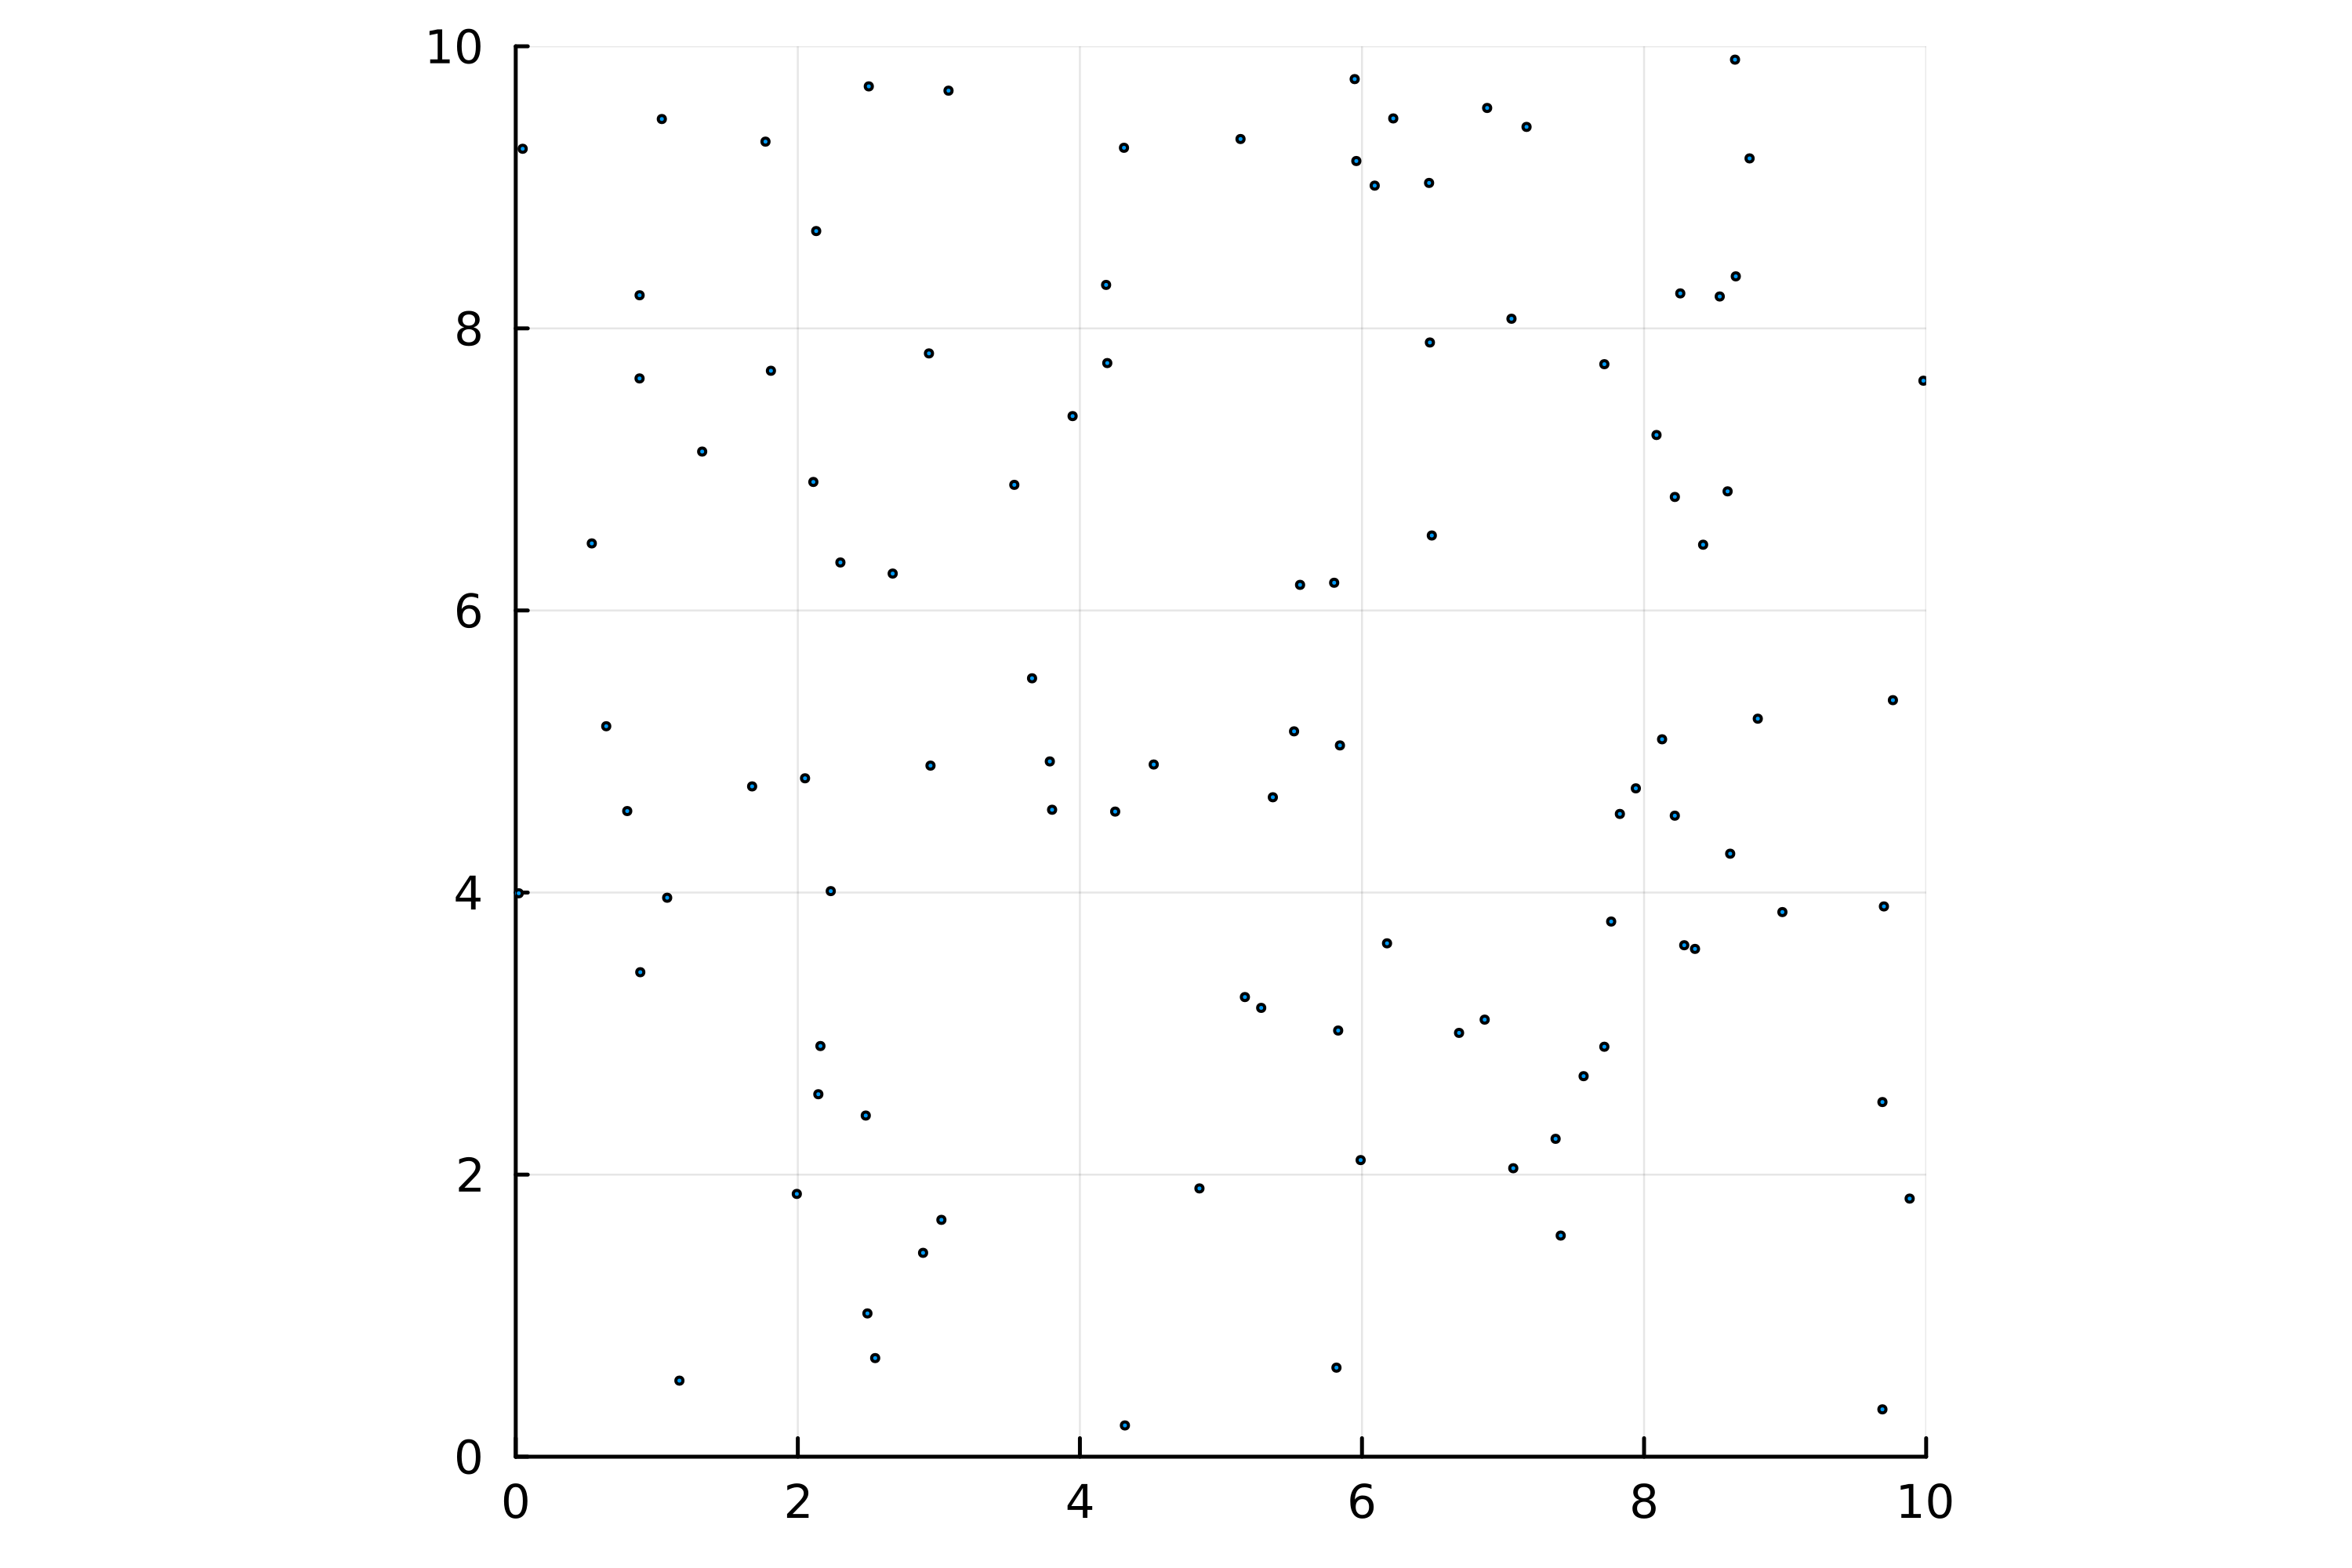
\includegraphics[width=\textwidth]{model_illustrations/particleModel.png}
		\caption{Here, one can see a possible snapshot of the point particle model that is explained at the beginning. The particles are randomly distributed in $\Omega$. The execution of the Brownian motion will cause the particle density to change according to the Diffusion equation.}
	\end{subfigure}
	\hfill
	\begin{subfigure}{0.4\textwidth}
		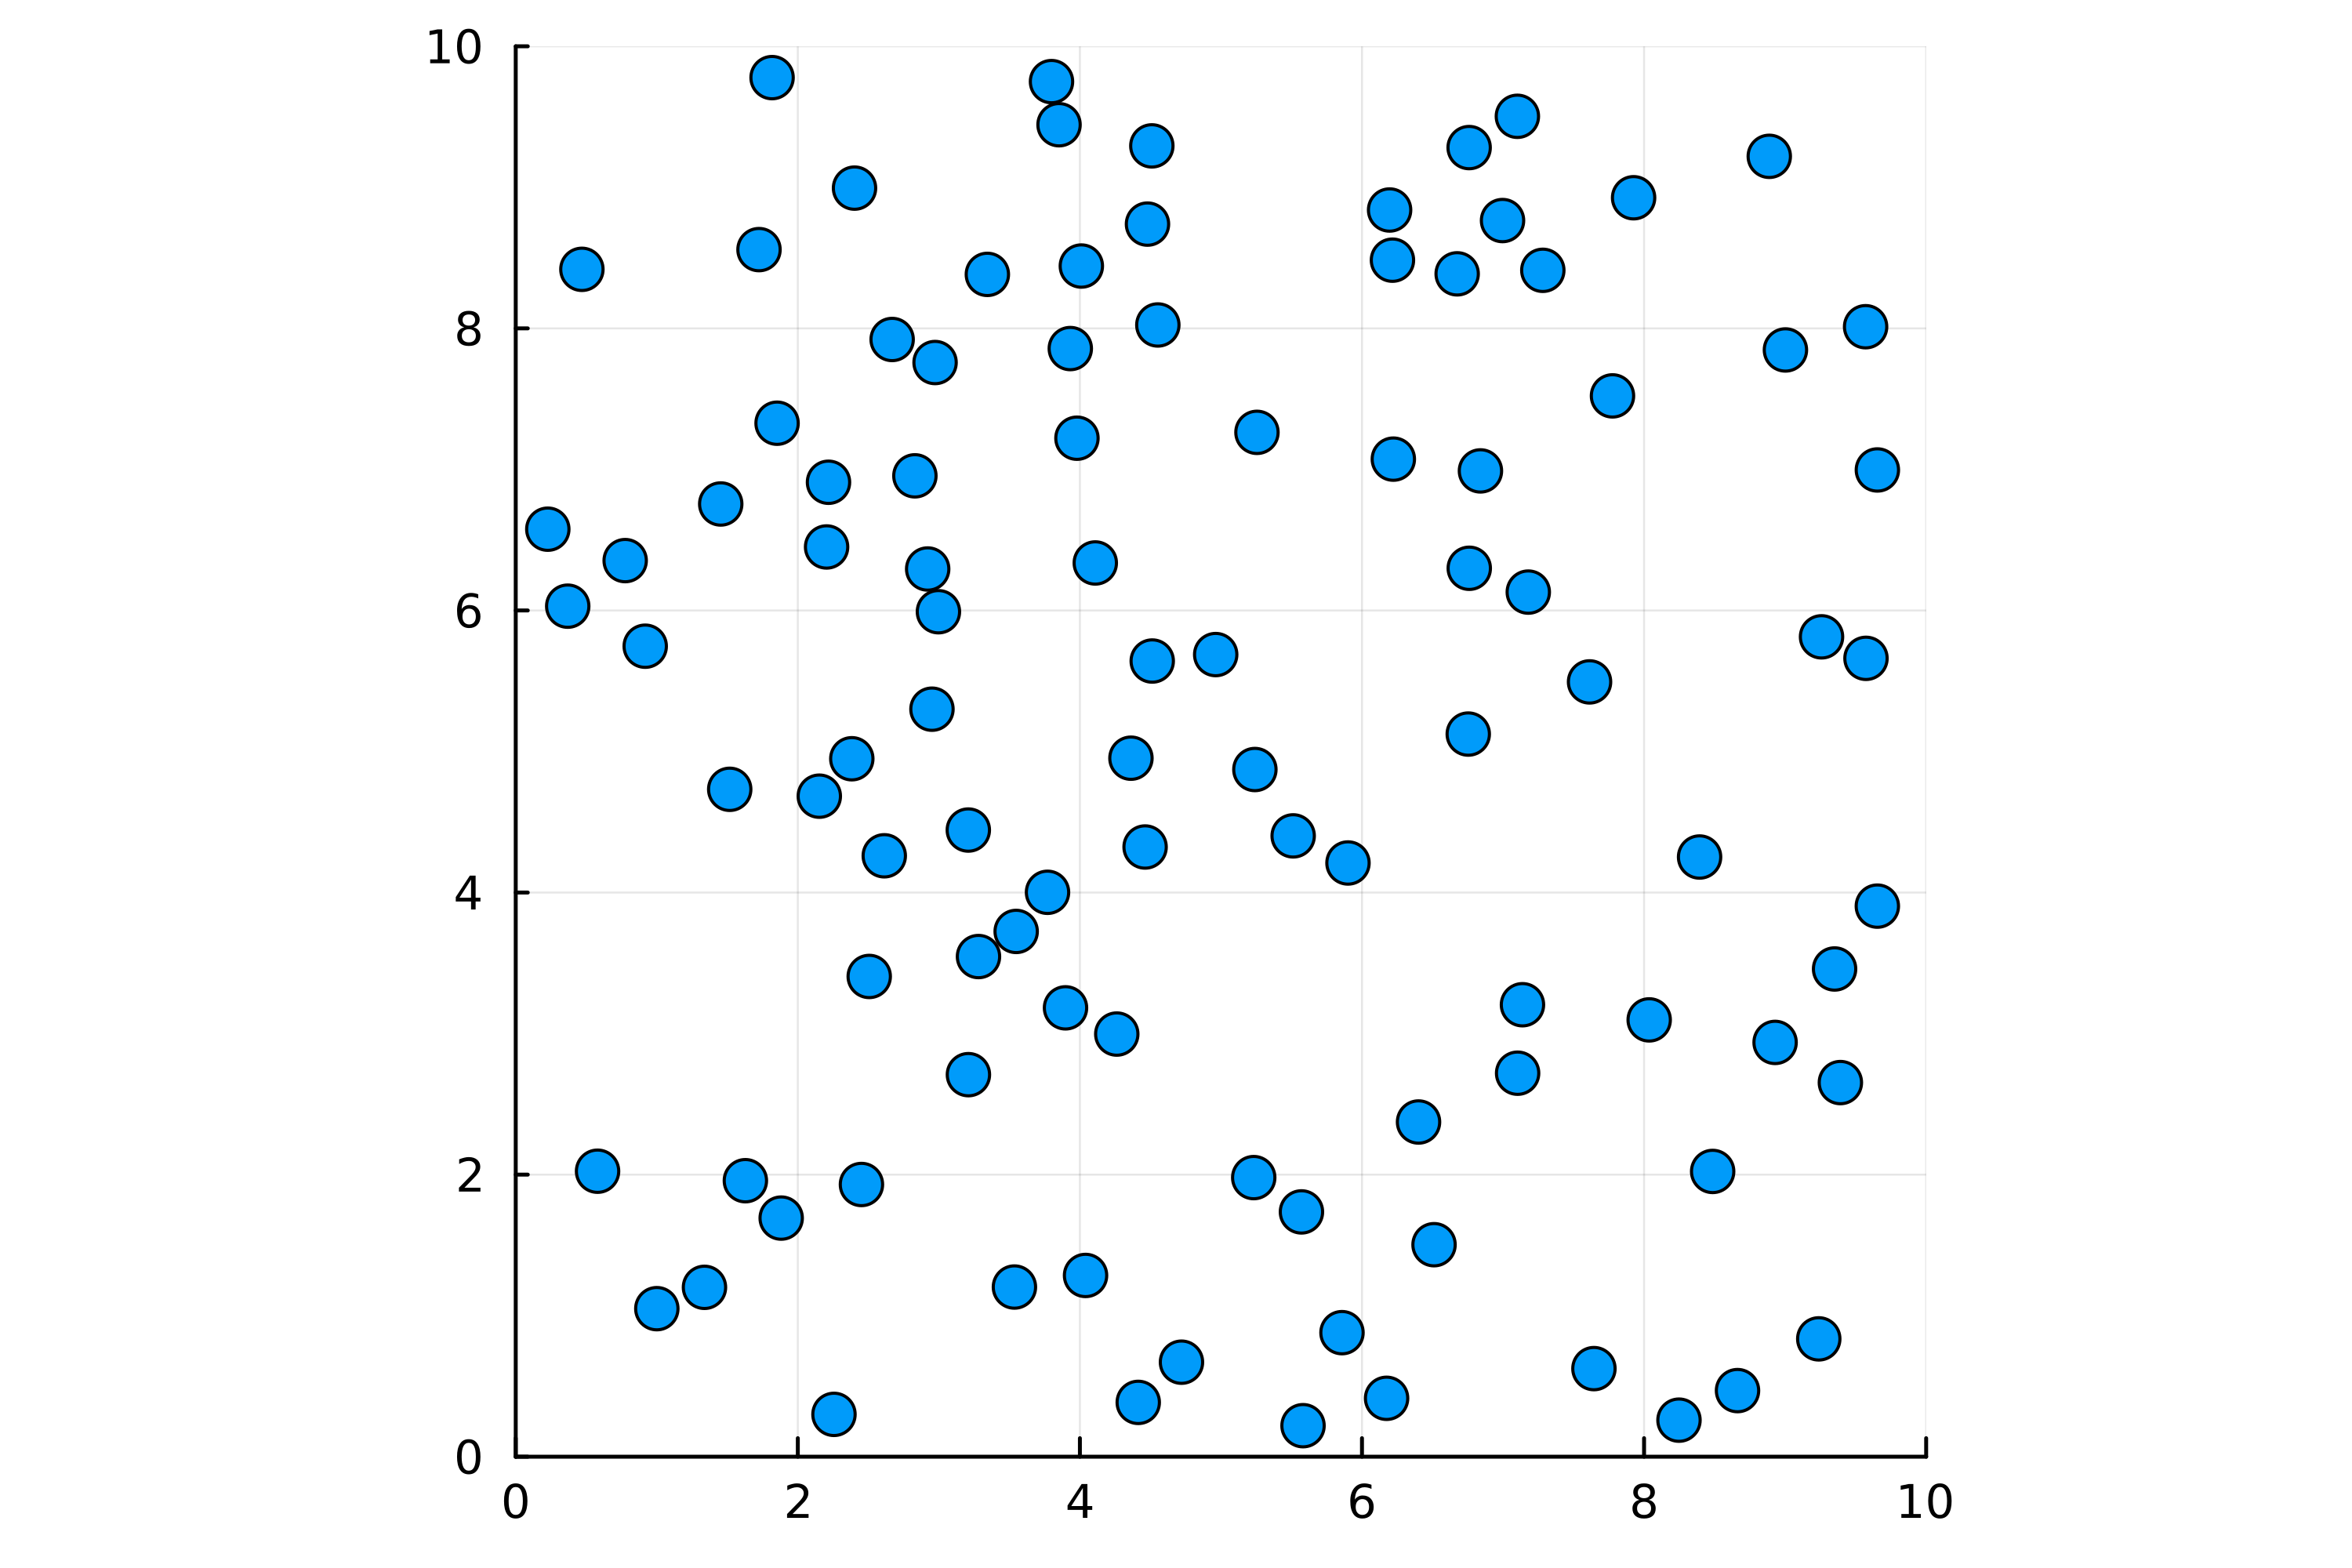
\includegraphics[width=\textwidth]{model_illustrations/SphereModel.png}
		\caption{In contrast to Figure (a), the particles do have a real radius in the sphere models. This causes particle interaction terms as addition in the particle movement, since particles can now collide. The type of interaction terms determines whether it is a hardsphere or softsphere model.   }
	\end{subfigure}
	\hfill
	\begin{subfigure}{0.4\textwidth}
		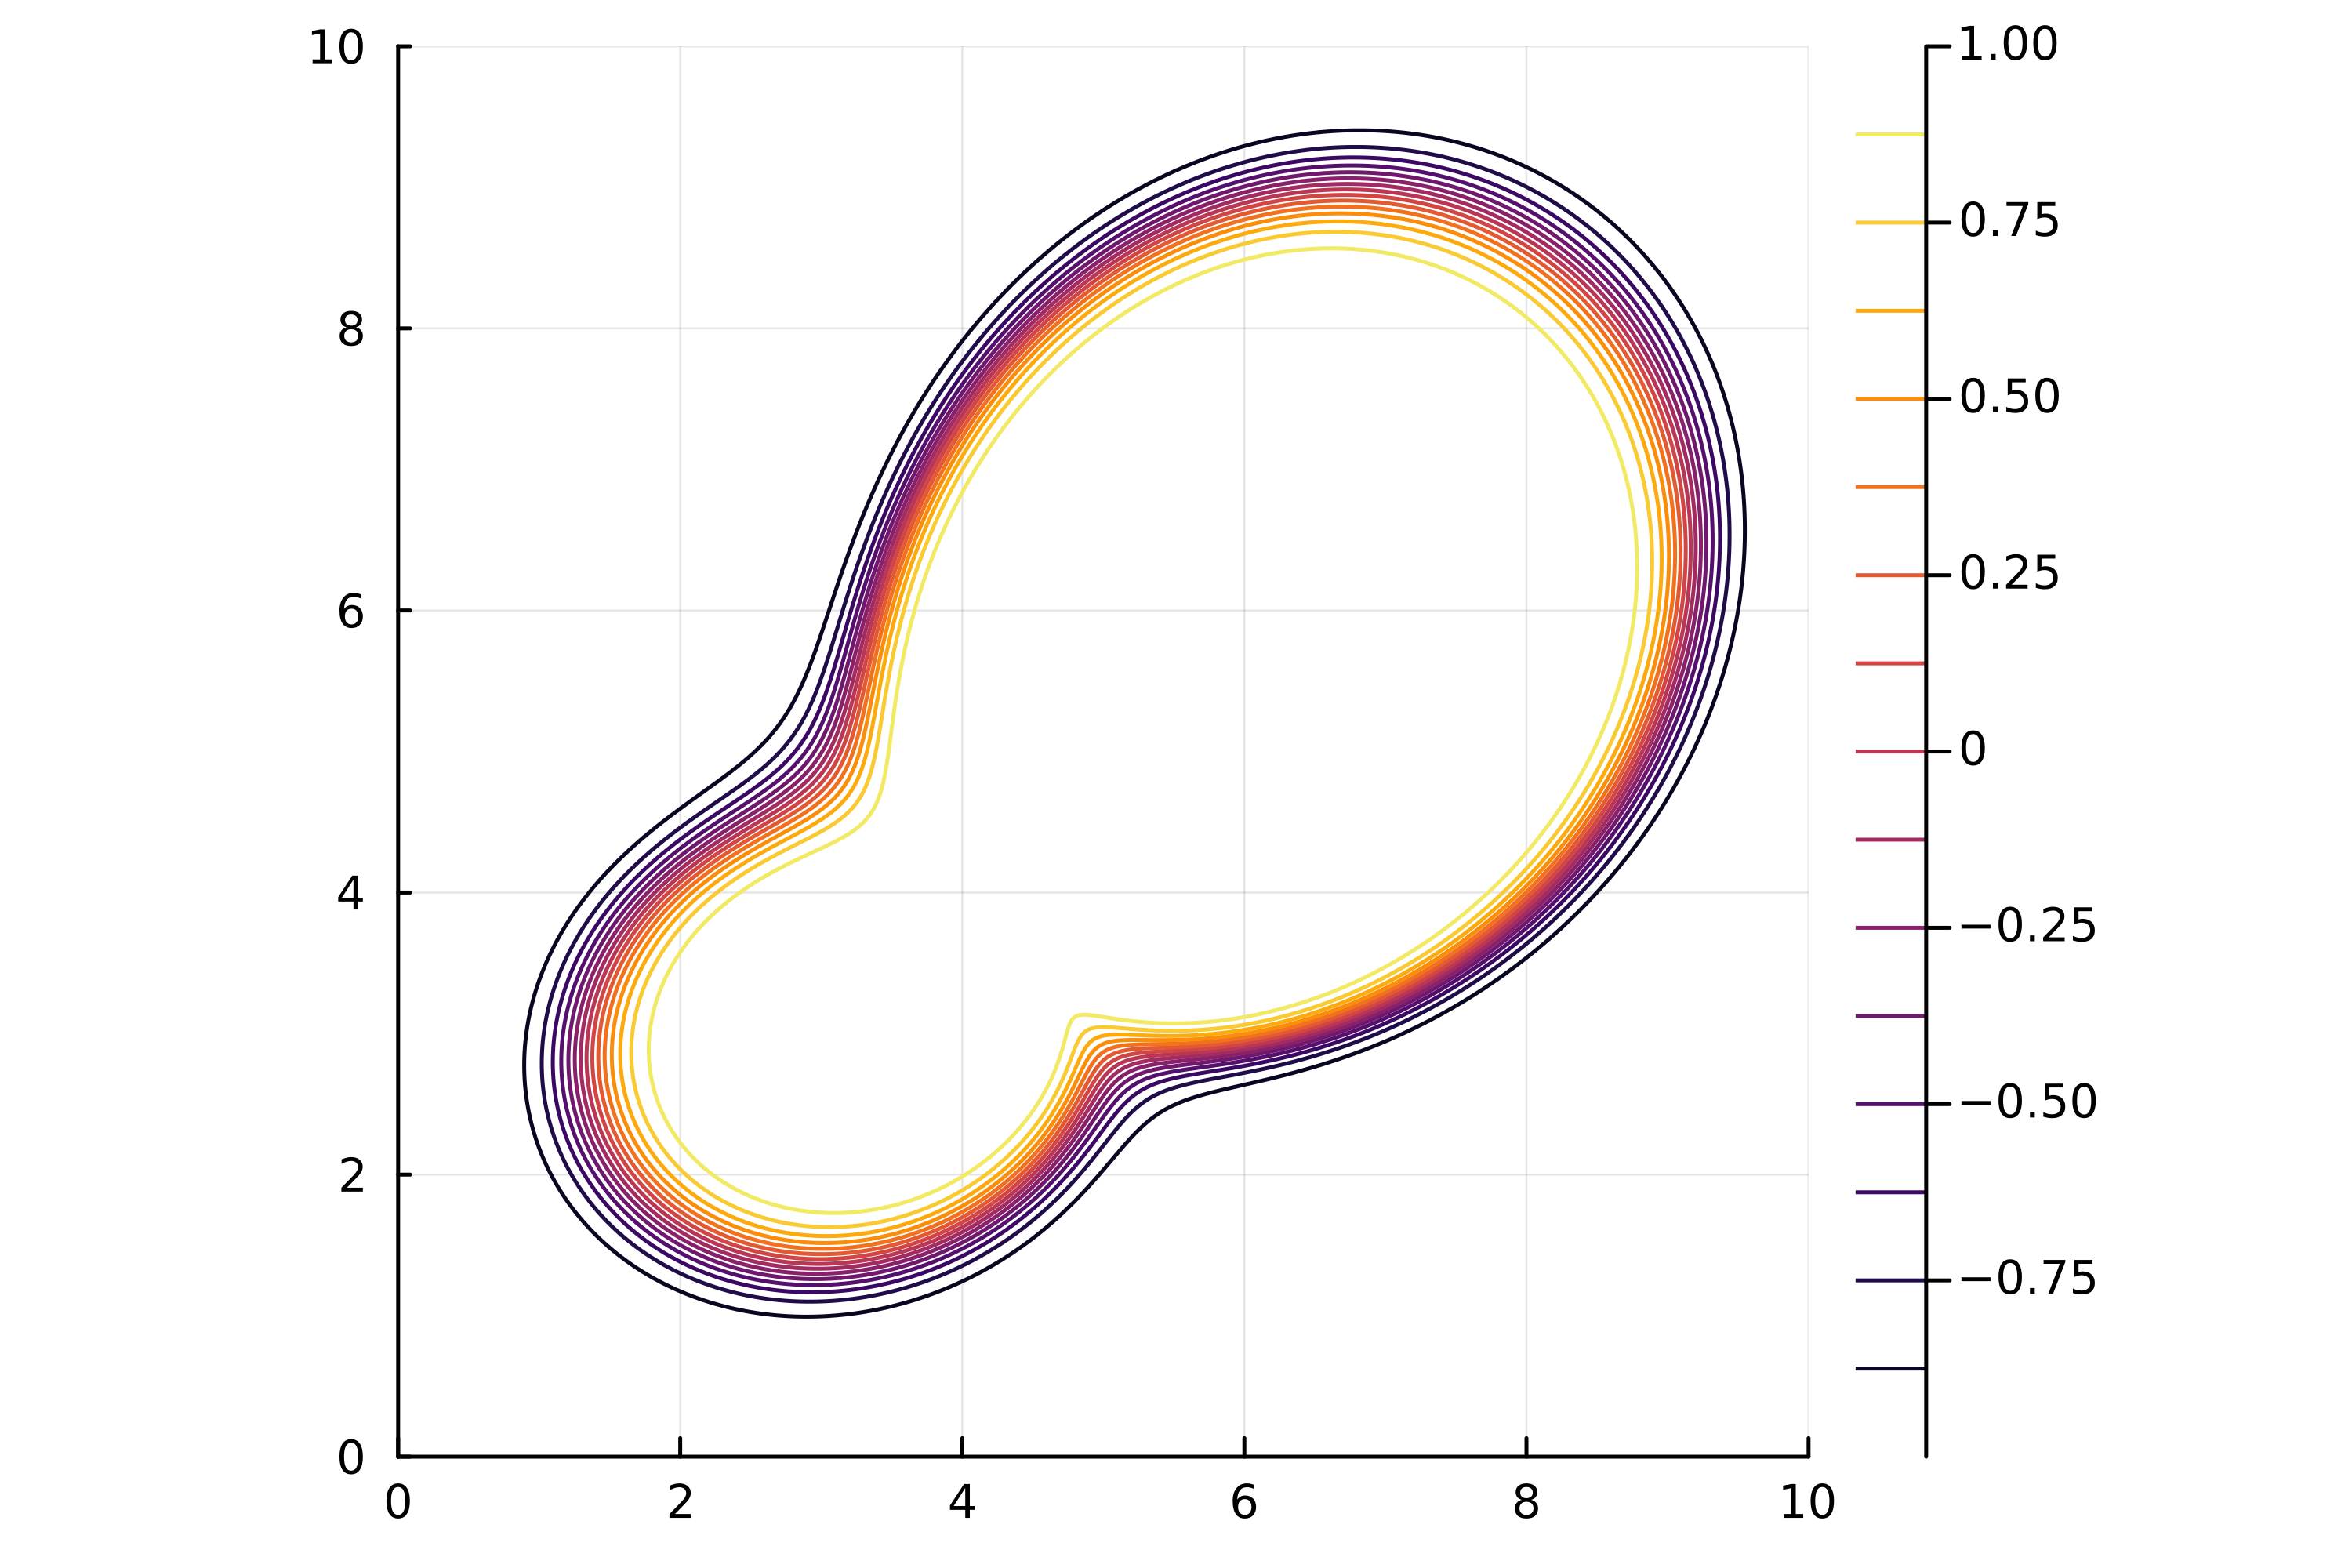
\includegraphics[width=\textwidth]{model_illustrations/PhaseFieldModel.png}
		\caption{A contour plot of a phase field variable $\phi$ illustrates how cells can be modeled through phase field models. The cell's inside is the area where $\phi > 0$. The cell wall sits on the red line where $\phi = 0$. The outer lines display the smooth transition to the outside. }
	\end{subfigure}\hfill
	\begin{subfigure}{0.4\textwidth}
		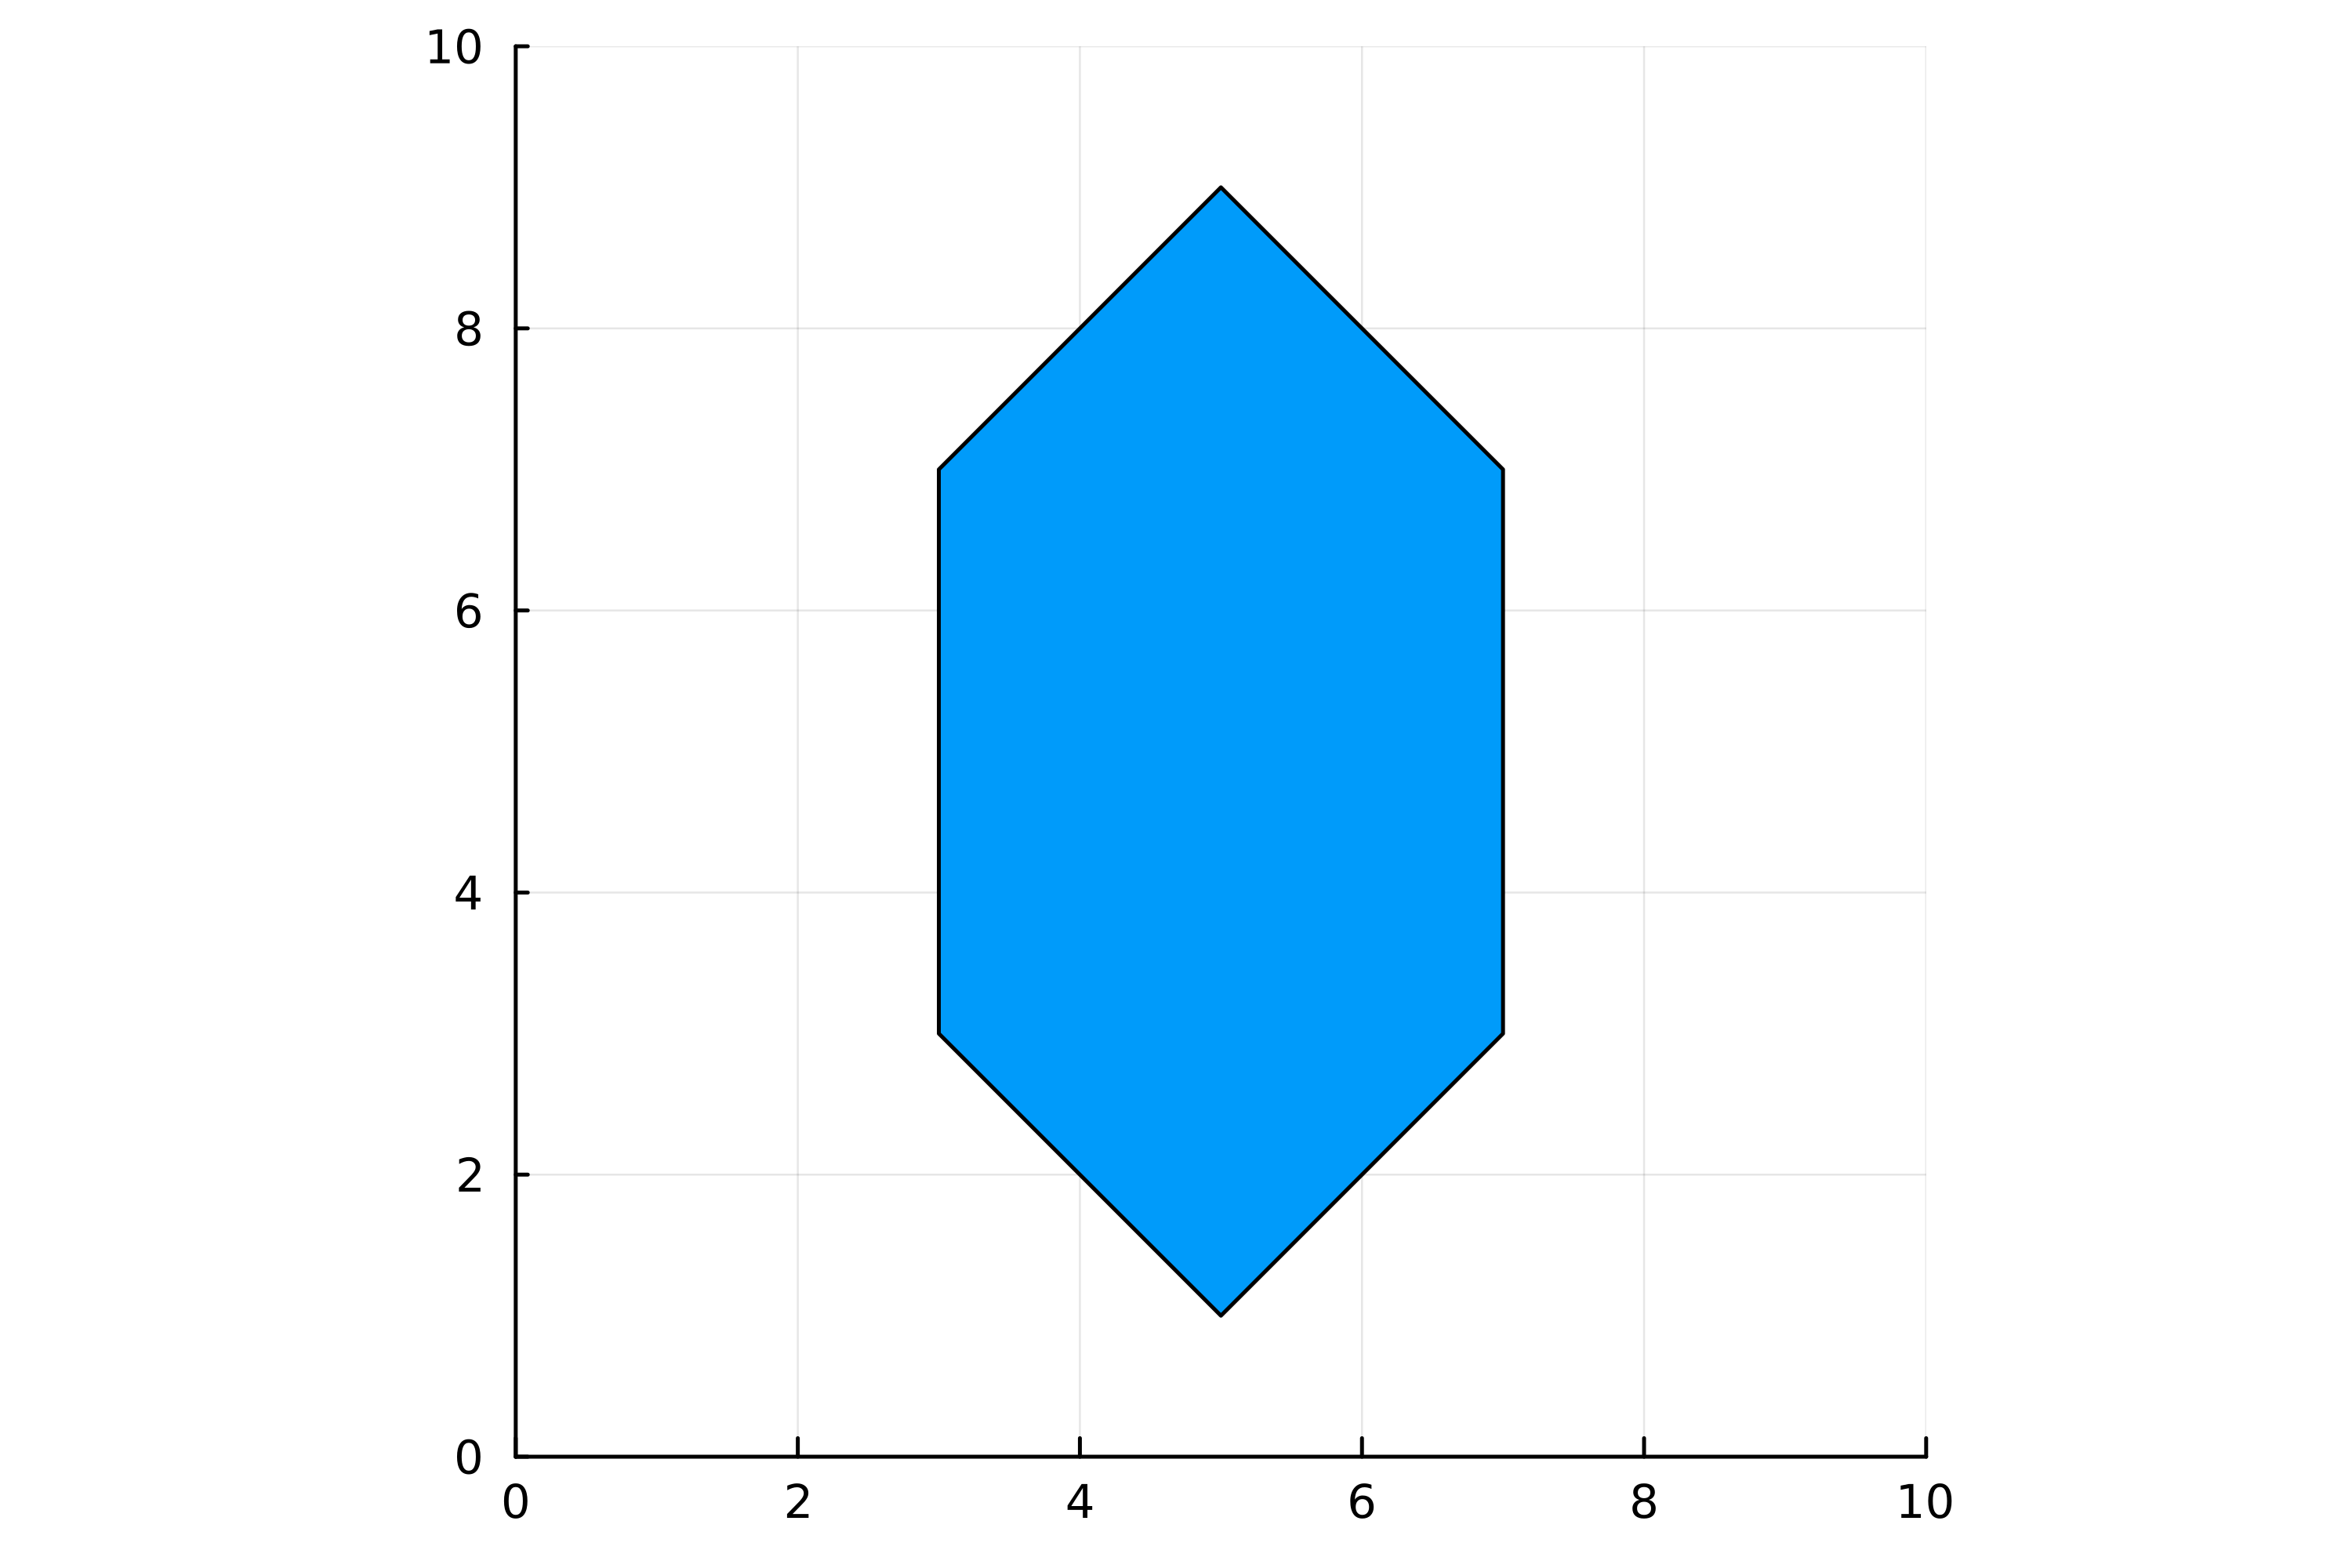
\includegraphics[width=\textwidth]{model_illustrations/VertexModel.png}
		\caption{Another possibility to model cell forms are Vertex models. An example of this is shown here. This cell has six vertices. In order to model cell deformations, one can define forces that act on each vertex separately and thus cause them to move in an according direction. }
	\end{subfigure}
	\caption{ To illustrate the models from the introduction, we can see a corresponding plot for each model. In (a) and (b) the focus is more on the density distribution of the particles in $\Omega$. The amount of particles is $N = 100$. The remaining sub figures (c) and (d) are concerned with the representation of cell shapes. In all sub figures, the axes denote the spatial $x$ and $y$ coordinates. } 
	\label{fig:model_illus}
\end{figure}
While the models presented only deal with spherical particles, in this thesis a large variety of shapes should be able to be modeled. The shape of a cell is another property that can influence the change in particle density over time in the domain. More complex shapes can be represented as in the model below, which can be assigned to the category of phase field models.  \\
Such a model is presented in \cite{Happel2023}. Here, each cell is modeled via a two dimensional phase field variable which is a smooth, continuous function $\phi_i \in [-1, 1]$, $(1 \leq i \leq N)$. Vectors $\vec{x}$ with positive values in $\phi_i$ are interior of the cell $i$ and all vectors with a negative value are considered to be exterior. Values of $\phi_i = 0$ denote the cell wall. The dynamic for each $\phi_i$ reads
\begin{align}
	\dfrac{ \partial \phi_i}{ \partial t} + v_0(\textbf{v}_i \cdot \nabla_{\vec{x}} \phi_i) = \Delta_{\vec{x}} \dfrac{\delta F}{\delta \phi_i}, \qquad 1 \leq i \leq N \label{eq:phasefield},
\end{align}
where $\textbf{v}_i$ is a vector field used to incorporate activity, with a self propulsion strength $v_0$, $F$ is a free energy and $\dfrac{\delta F}{\delta \phi_i}$ denotes the first variation. $F$ results from a sum of different energies which are e.g. used to ensure that $\phi_i$ stays between $-1$ and $1$, that the cell keeps a certain shape, or that the different cell interactions are correctly included. \\
An easier approach to model cell shapes are vertex models, like for example in \cite{Fletcher14}.
Vertex models are part of a broader class of computational models used in computational biology and biophysics to study the biomechanics and behavior of cells and tissues. They are valuable tools for understanding how cells respond to mechanical cues and how their behavior contributes to biological processes. In a vertex model of a cell, the cell's outline or boundary is approximated as a polygon. The vertices of this polygon represent discrete points along the cell's boundary. Movements or transformations of the cell are given by forces that are applied on each vertex individually. In \cite{Fletcher14} the cell dynamic reads 
\begin{align}
	\eta \dfrac{d \vec{x}_i}{dt} = F_i, \qquad 1 \leq i \leq N \label{eq:vertexmodel}, 
\end{align}
where $\eta$ is a scaling factor and $F_i$ is the total force acting on $\vec{x}_i$. Like in the phase field model, $F_i$ is a sum of different forces that define the cell behavior, such as the cell flexibility or the interaction with other cells.  \\
The aim of this work is to introduce mathematical models of cells that can cover a wide range of shapes like the models in \cite{Happel2023} and also in \cite{Fletcher14}. We also want to derive forces that are applicable to the new models and that have an influence on the diffusion behavior of the cell systems as in \cite{Bruna2012} and \cite{Bruna2017}. \\
Section \ref{sec:CellDef} defines such models, named centre radius form (CRF) and discrete form (DF). It also gives some functionalities that will be needed in order to implement desired cell actions and interactions. \\
On one hand, the CRF represents a continuous form of a cell. A centre point and a radius function allow a precise representation of the cell in which any number of wall points can be calculated. Every bounded and star shaped domain that has a smooth boundary can be expressed via a CRF. The smooth indicator function, used to plot CRF cells and compute their areas or cell overlaps, has similarities to a phase field variable described in \cite{Happel2023}. In Section \ref{sec:ShapeRecoveryModel} a dynamic is introduced that allows the transition from one CRF to another. \\
On the other hand, we have got DF cells. This is a vertex model, similar to the model considered in \cite{Fletcher14}. Various forces and interactions between the vertices and cells are modeled to simulate cell behavior in Section \ref{sec:energyModels}. \\
At the end of this thesis, advantages and disadvantages of the introduced models, as well as possible improvements and extensions are discussed in the conclusion. \\
A large part of the development of this thesis is the implementation and simulation of the cell forms and their dynamics. The Julia programming language is used for this. Julia offers advantages such as high performance numerical computing, easy integration with existing code written in languages like C and Fortran and a user friendly syntax for rapid development of scientific and data analysis applications. \\
Hereinafter, any points $\vec{x} \in \R^d$ ($d \in \N_{>1}$) are written with a superscript arrow. The line segment between two points $\vec{x}, \vec{y} \in \R^d$ is expressed through the notation $\overline{\vec{x} \: \vec{y}}$.



\newpage
\section{Cell definitions and area computations} \label{sec:CellDef}
Before we are able to run programs and simulate cell behavior, we must first set a definition of what exactly a cell is, i.e. how we want to model them. Thus, this section will give such a simplified mathematical model of a cell. \\
In this thesis, we will always consider the the two dimensional space of real numbers. Consequently, a cell will always be embedded in $\R^2$. 
Since we want to take a look at the development of the cell shape, we want a model that provides as much freedom of shape as possible. Ergo, simple discs or other static geometric forms are not versatile enough. Instead, we take a look at the following approach. \\
\subsection{Continuous and discrete cell models} 
In the first approach, we define a cell by its centre point and a so called radius function which takes an angle $\phi \in [0, 2\pi)$ and returns the cell radius at that point. \\
\begin{figure}[b!]
	\begin{center}
		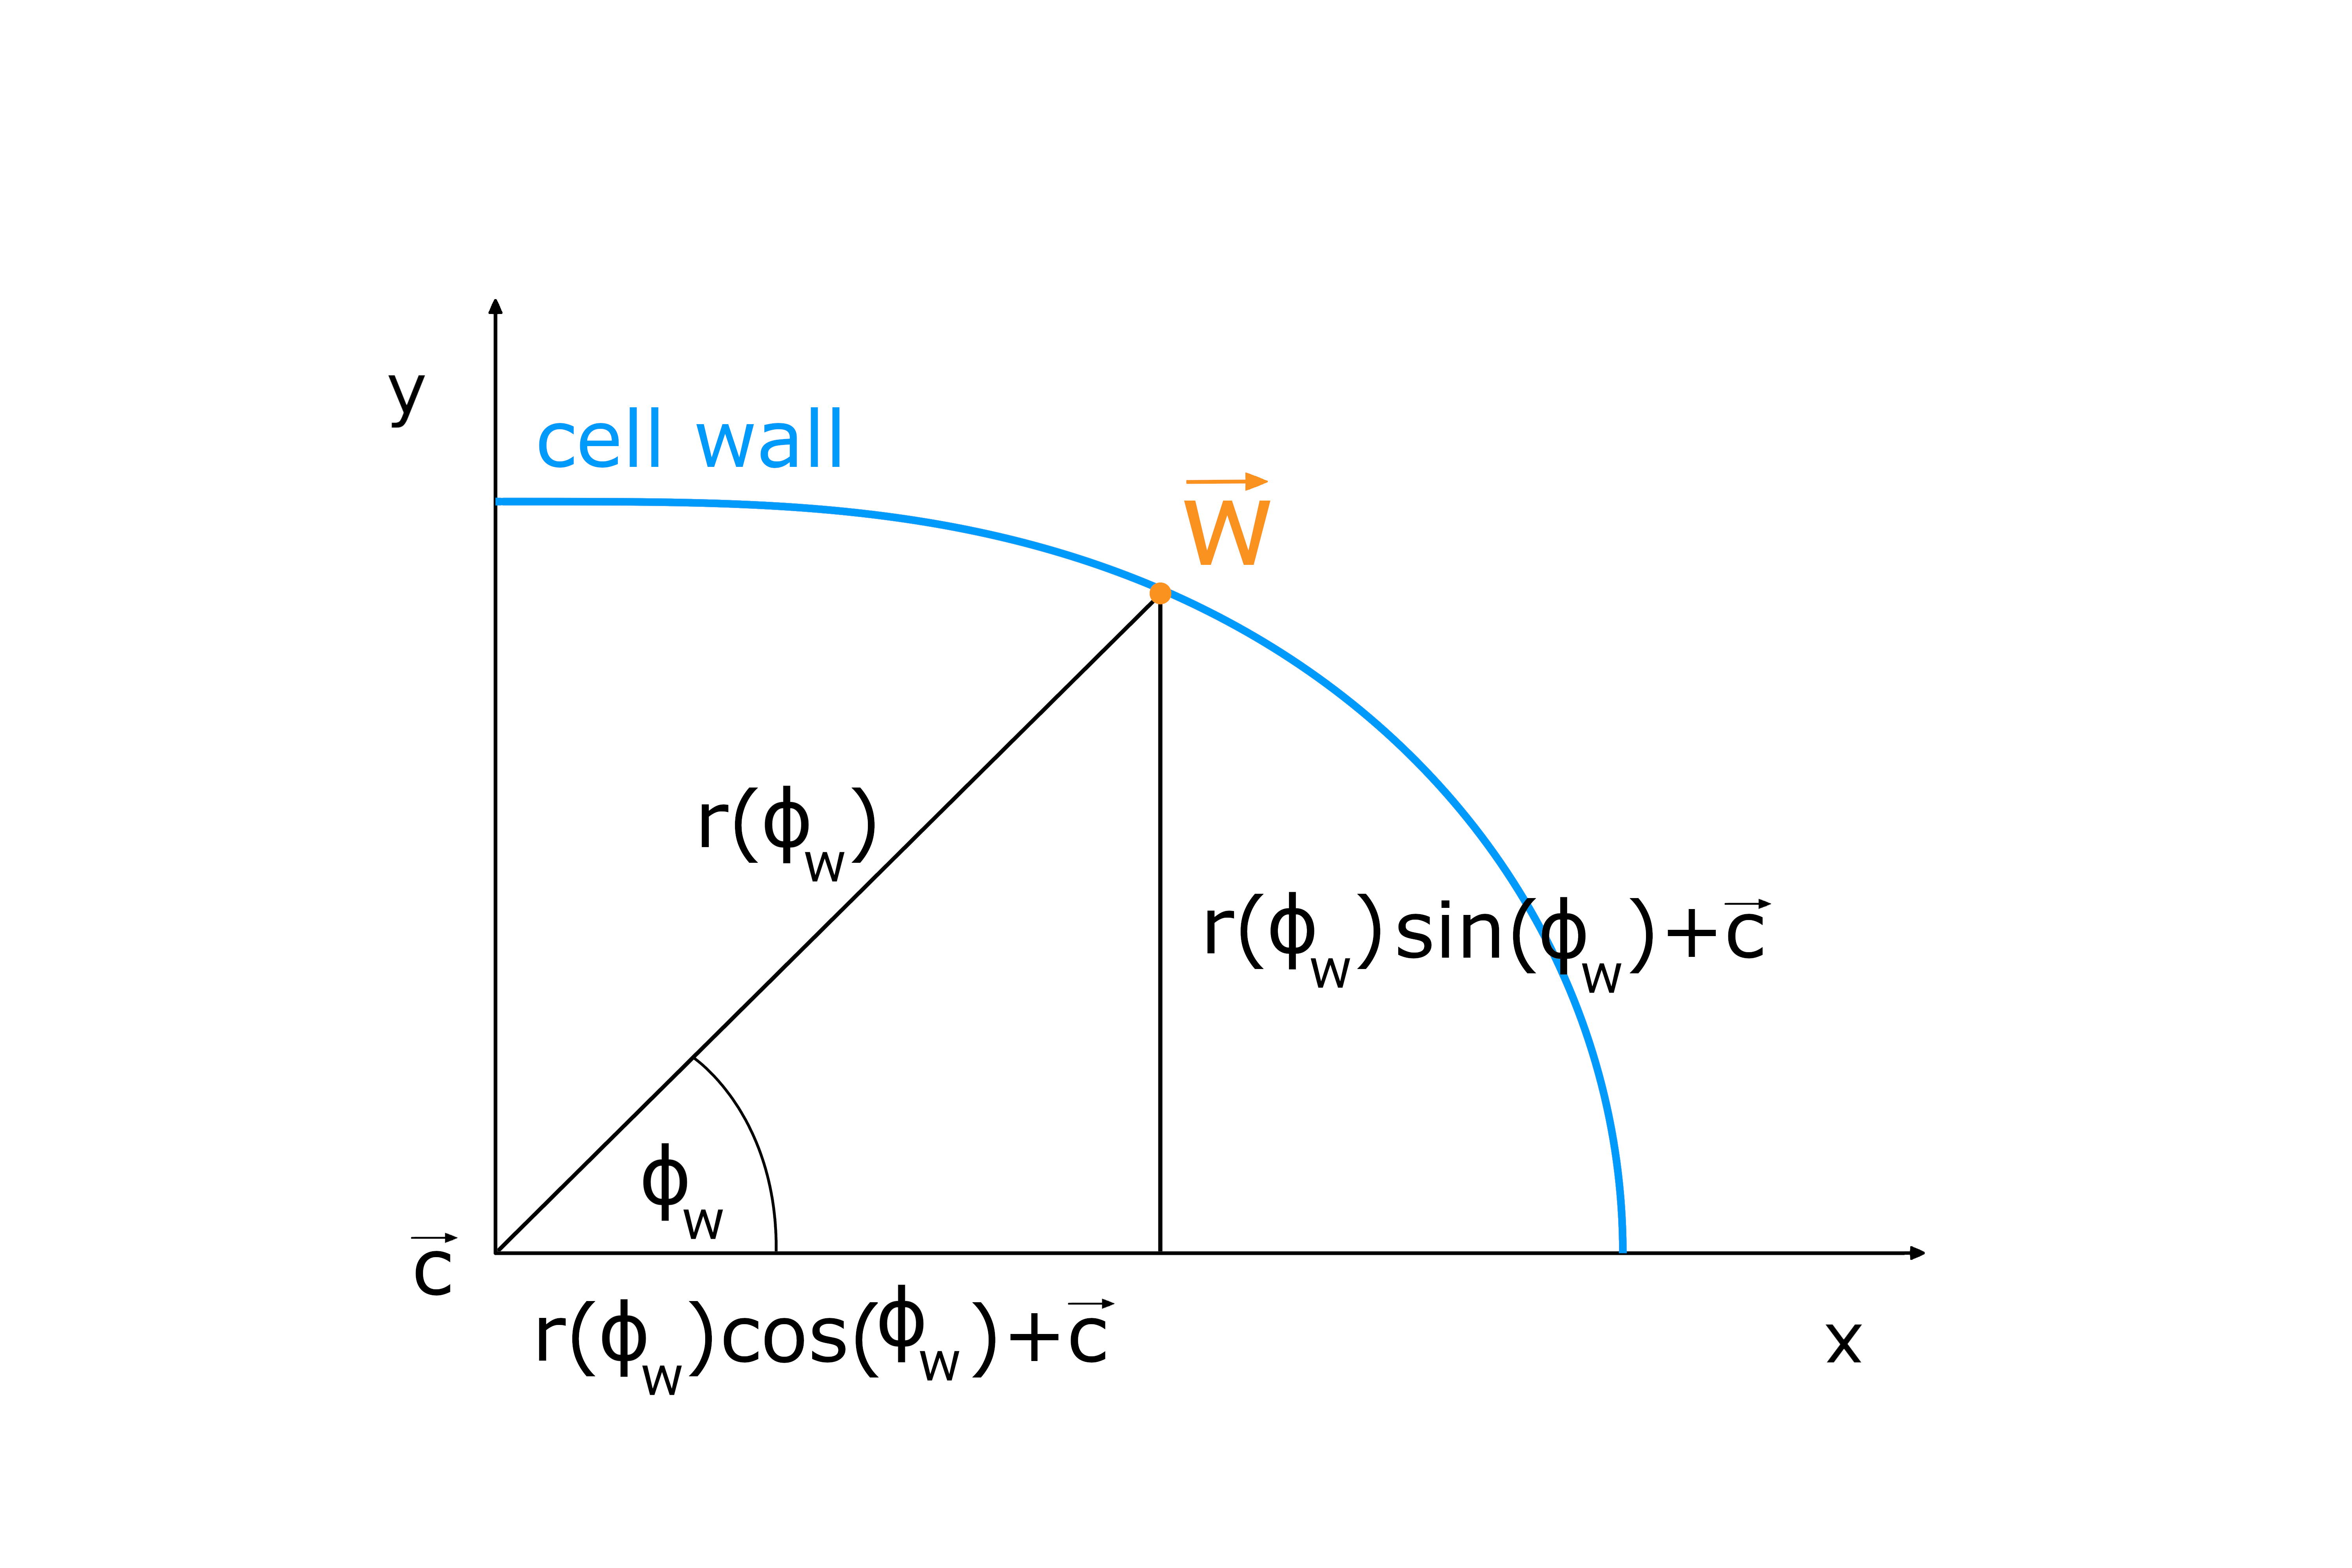
\includegraphics[width=8cm]{SketchCompWallPoint1.png}
		\caption{A sketch of the calculation of the $x$ and $y$ coordinates of a vertex of a cell in its CRF.}
		\label{fig:SketchCompWallPoint1}
	\end{center}
\end{figure}
\begin{definition} \textbf{Centre radius form (CRF)} \label{def:CRF}  \\
	For a given point $\vec{c} \in \mathbb{R}^2$ and function $r: [0, 2\pi) \rightarrow (0, \infty)$ so that $r \in C^1([0, 2\pi))$, $r(0) = r(2\pi)$ and $r'(0) = r'(2\pi)$, the tuple $(\vec{c}, r)$ describes a cell in its centre radius form (CRF) with centre point $\vec{c}$ and radius $r(\phi)$ at angle $\phi \in [0, 2\pi)$ that is taken with the $x$ axis. \\
\end{definition}
Since we want our cell wall to be smooth, it is a reasonable requirement to choose our radius function $r$ to be smooth as well. The boundary conditions ensure a soft transition at angle $\phi = 0$ or, respectively, $\phi = 2\pi$. 
With this form we are able to describe and plot cells that have a star shaped form and a smooth wall. One can easily imagine that there are also cell forms which are not star shaped and which cannot be displayed with the CRF. But hereinafter, we will just focus on the wide range of shapes that can be represented by a CRF cell. \\
For every point on the cell wall $\vec{w}$, we can draw a right triangle and then use the theorems on trigonometric functions in right triangles to compute
\begin{center}
	$\vec{w} = \begin{pmatrix} x \\ y \end{pmatrix} = r(\phi_{w}) \begin{pmatrix} \cos(\phi_{w}) \\ \sin(\phi_{w}) \end{pmatrix} + \vec{c}$, 
\end{center}
as we can see in Figure \ref{fig:SketchCompWallPoint1}.\\
In order to obtain our first plots, we just have to save an amount of vertices using this equation and then perform a shape plot with this list of points. Figure \ref{fig:plotExamples} shows us some examples. \\
Having established a continuous cell model, we are now also looking for a further simplification. The reason for this is that most cell dynamics in this thesis are applied on a vertex model in Section \ref{sec:energyModels}. It is straight forward to just use a sequence of vertices. First of all, we will introduce some definitions of two dimensional objects and their characteristics.\\
\begin{figure}[t!]
	\centering
	\begin{subfigure}{0.3\textwidth}
		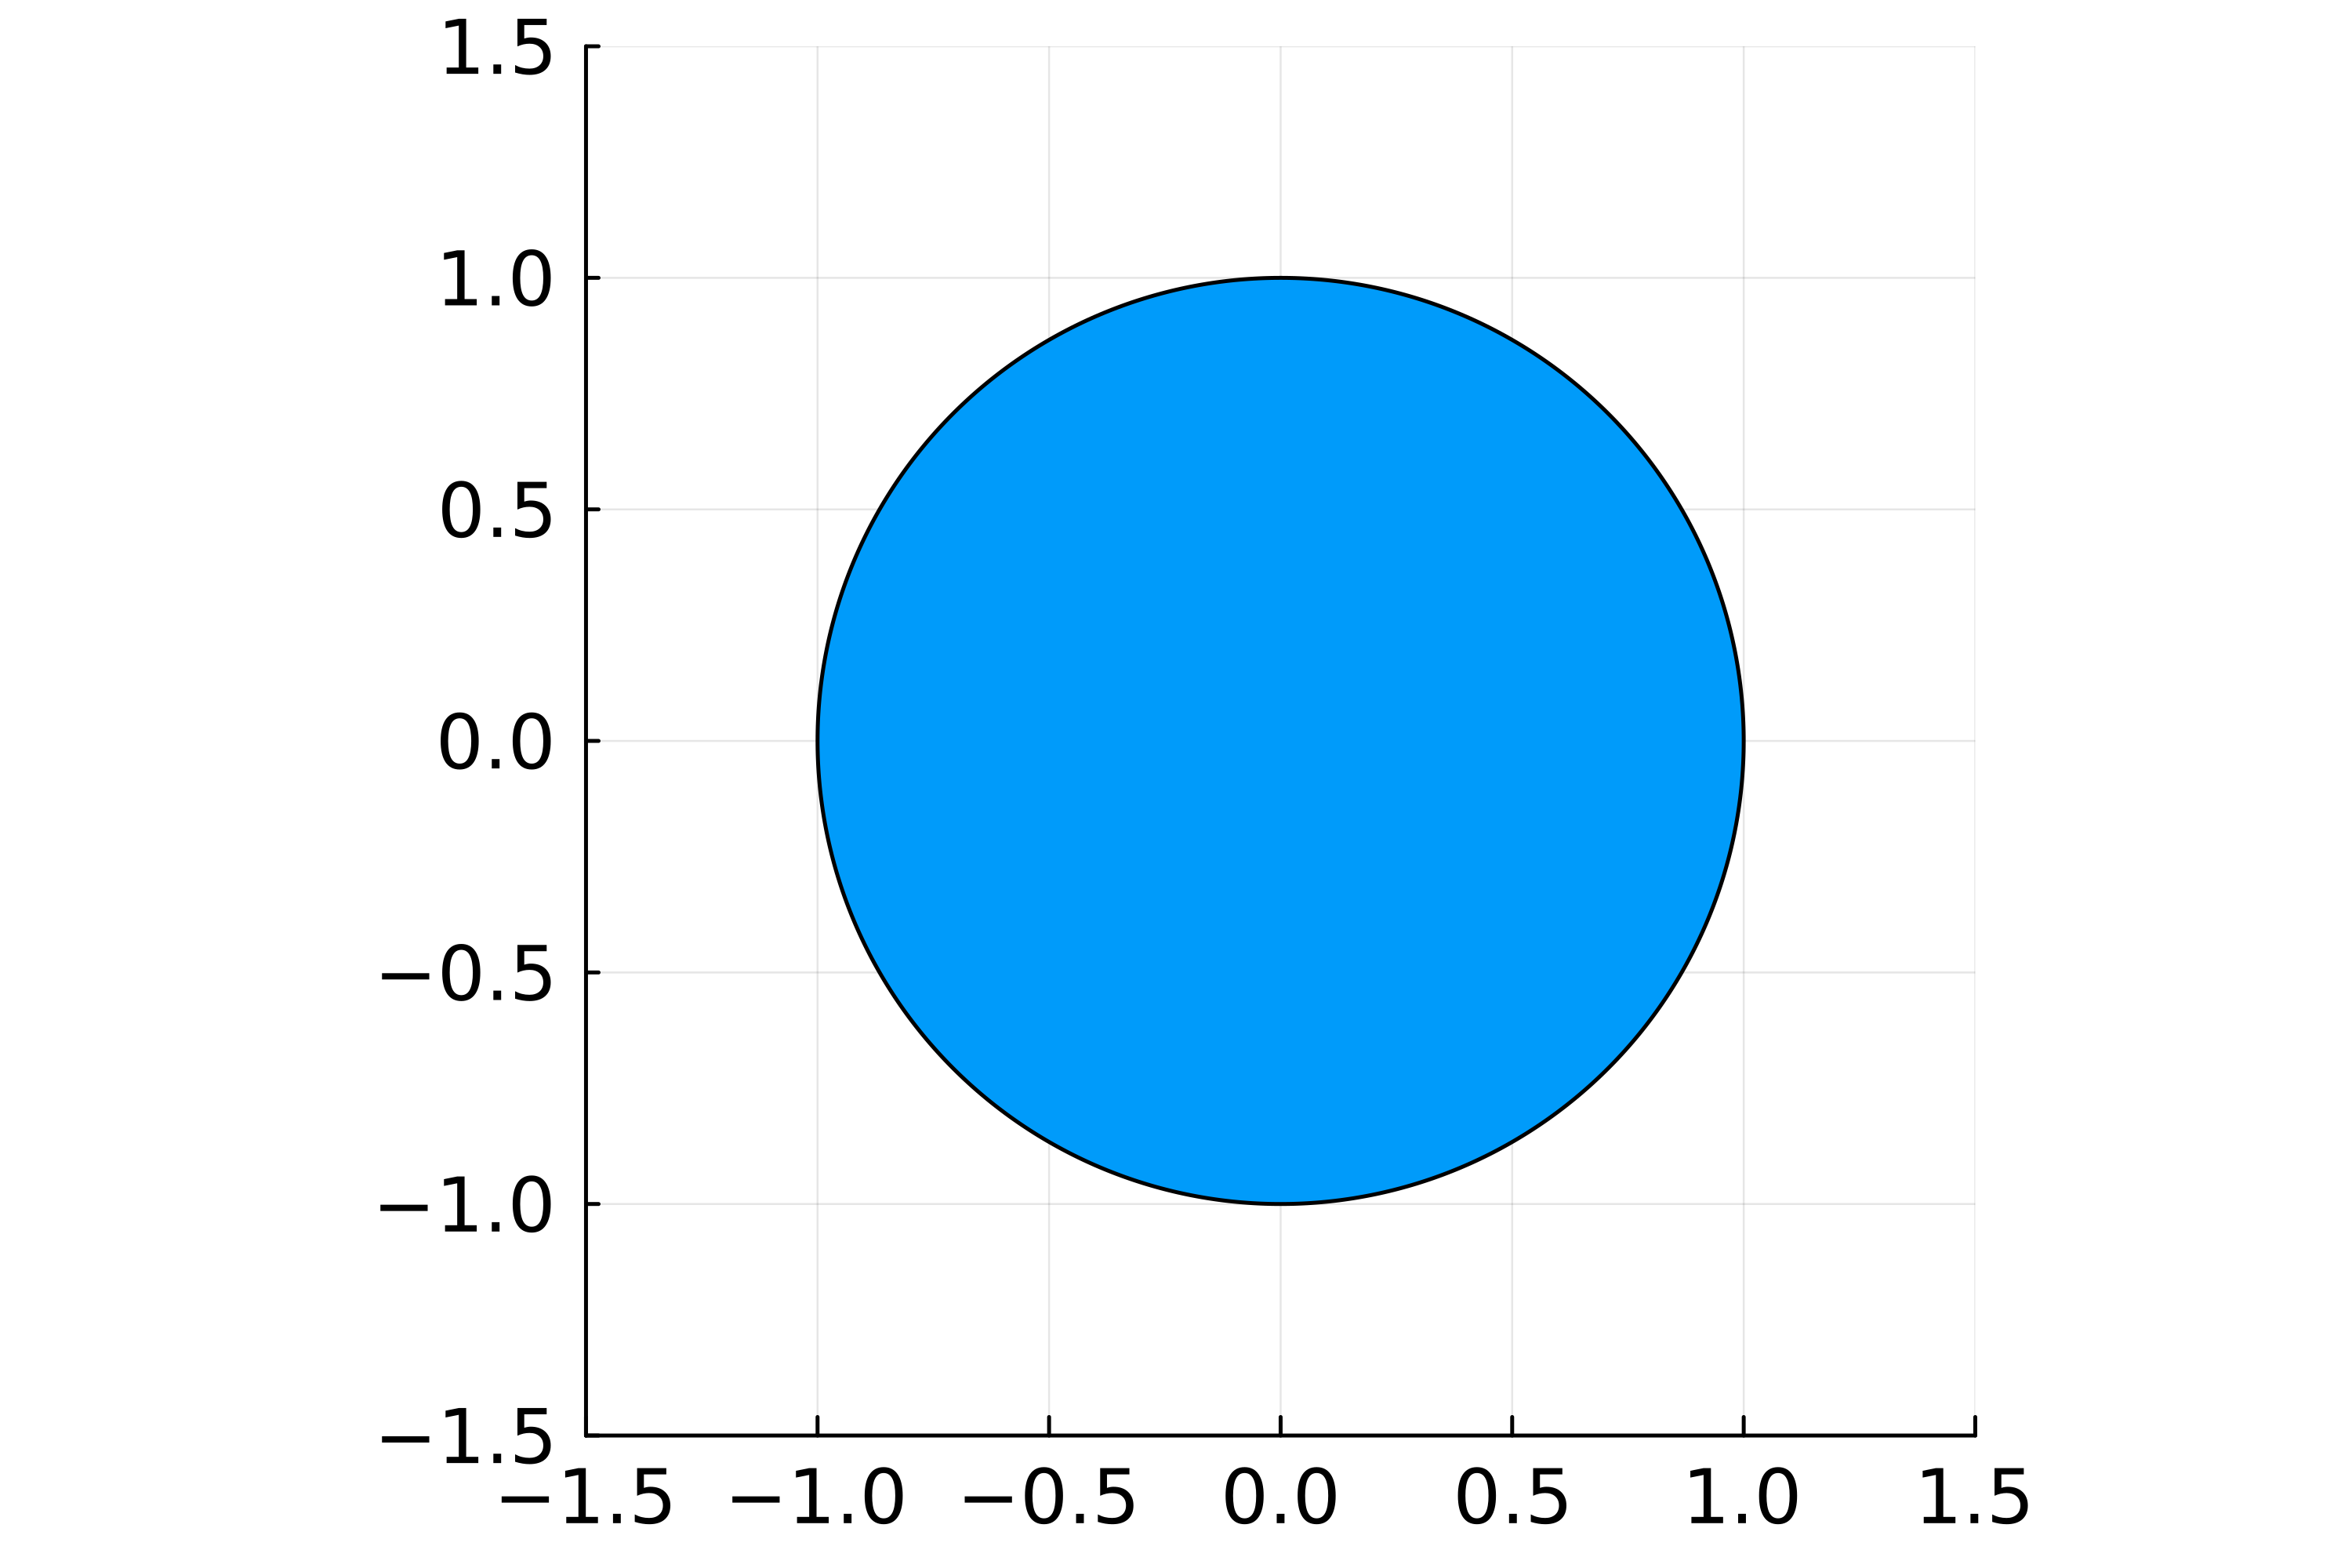
\includegraphics[width=\textwidth]{plotExample1_unitcircle.png}
		\caption{unit circle cell:  \\ $r_{a}(\phi) = 1$}
		\label{fig:unitcircle}
	\end{subfigure}
	\hfill
	\begin{subfigure}{0.3\textwidth}
		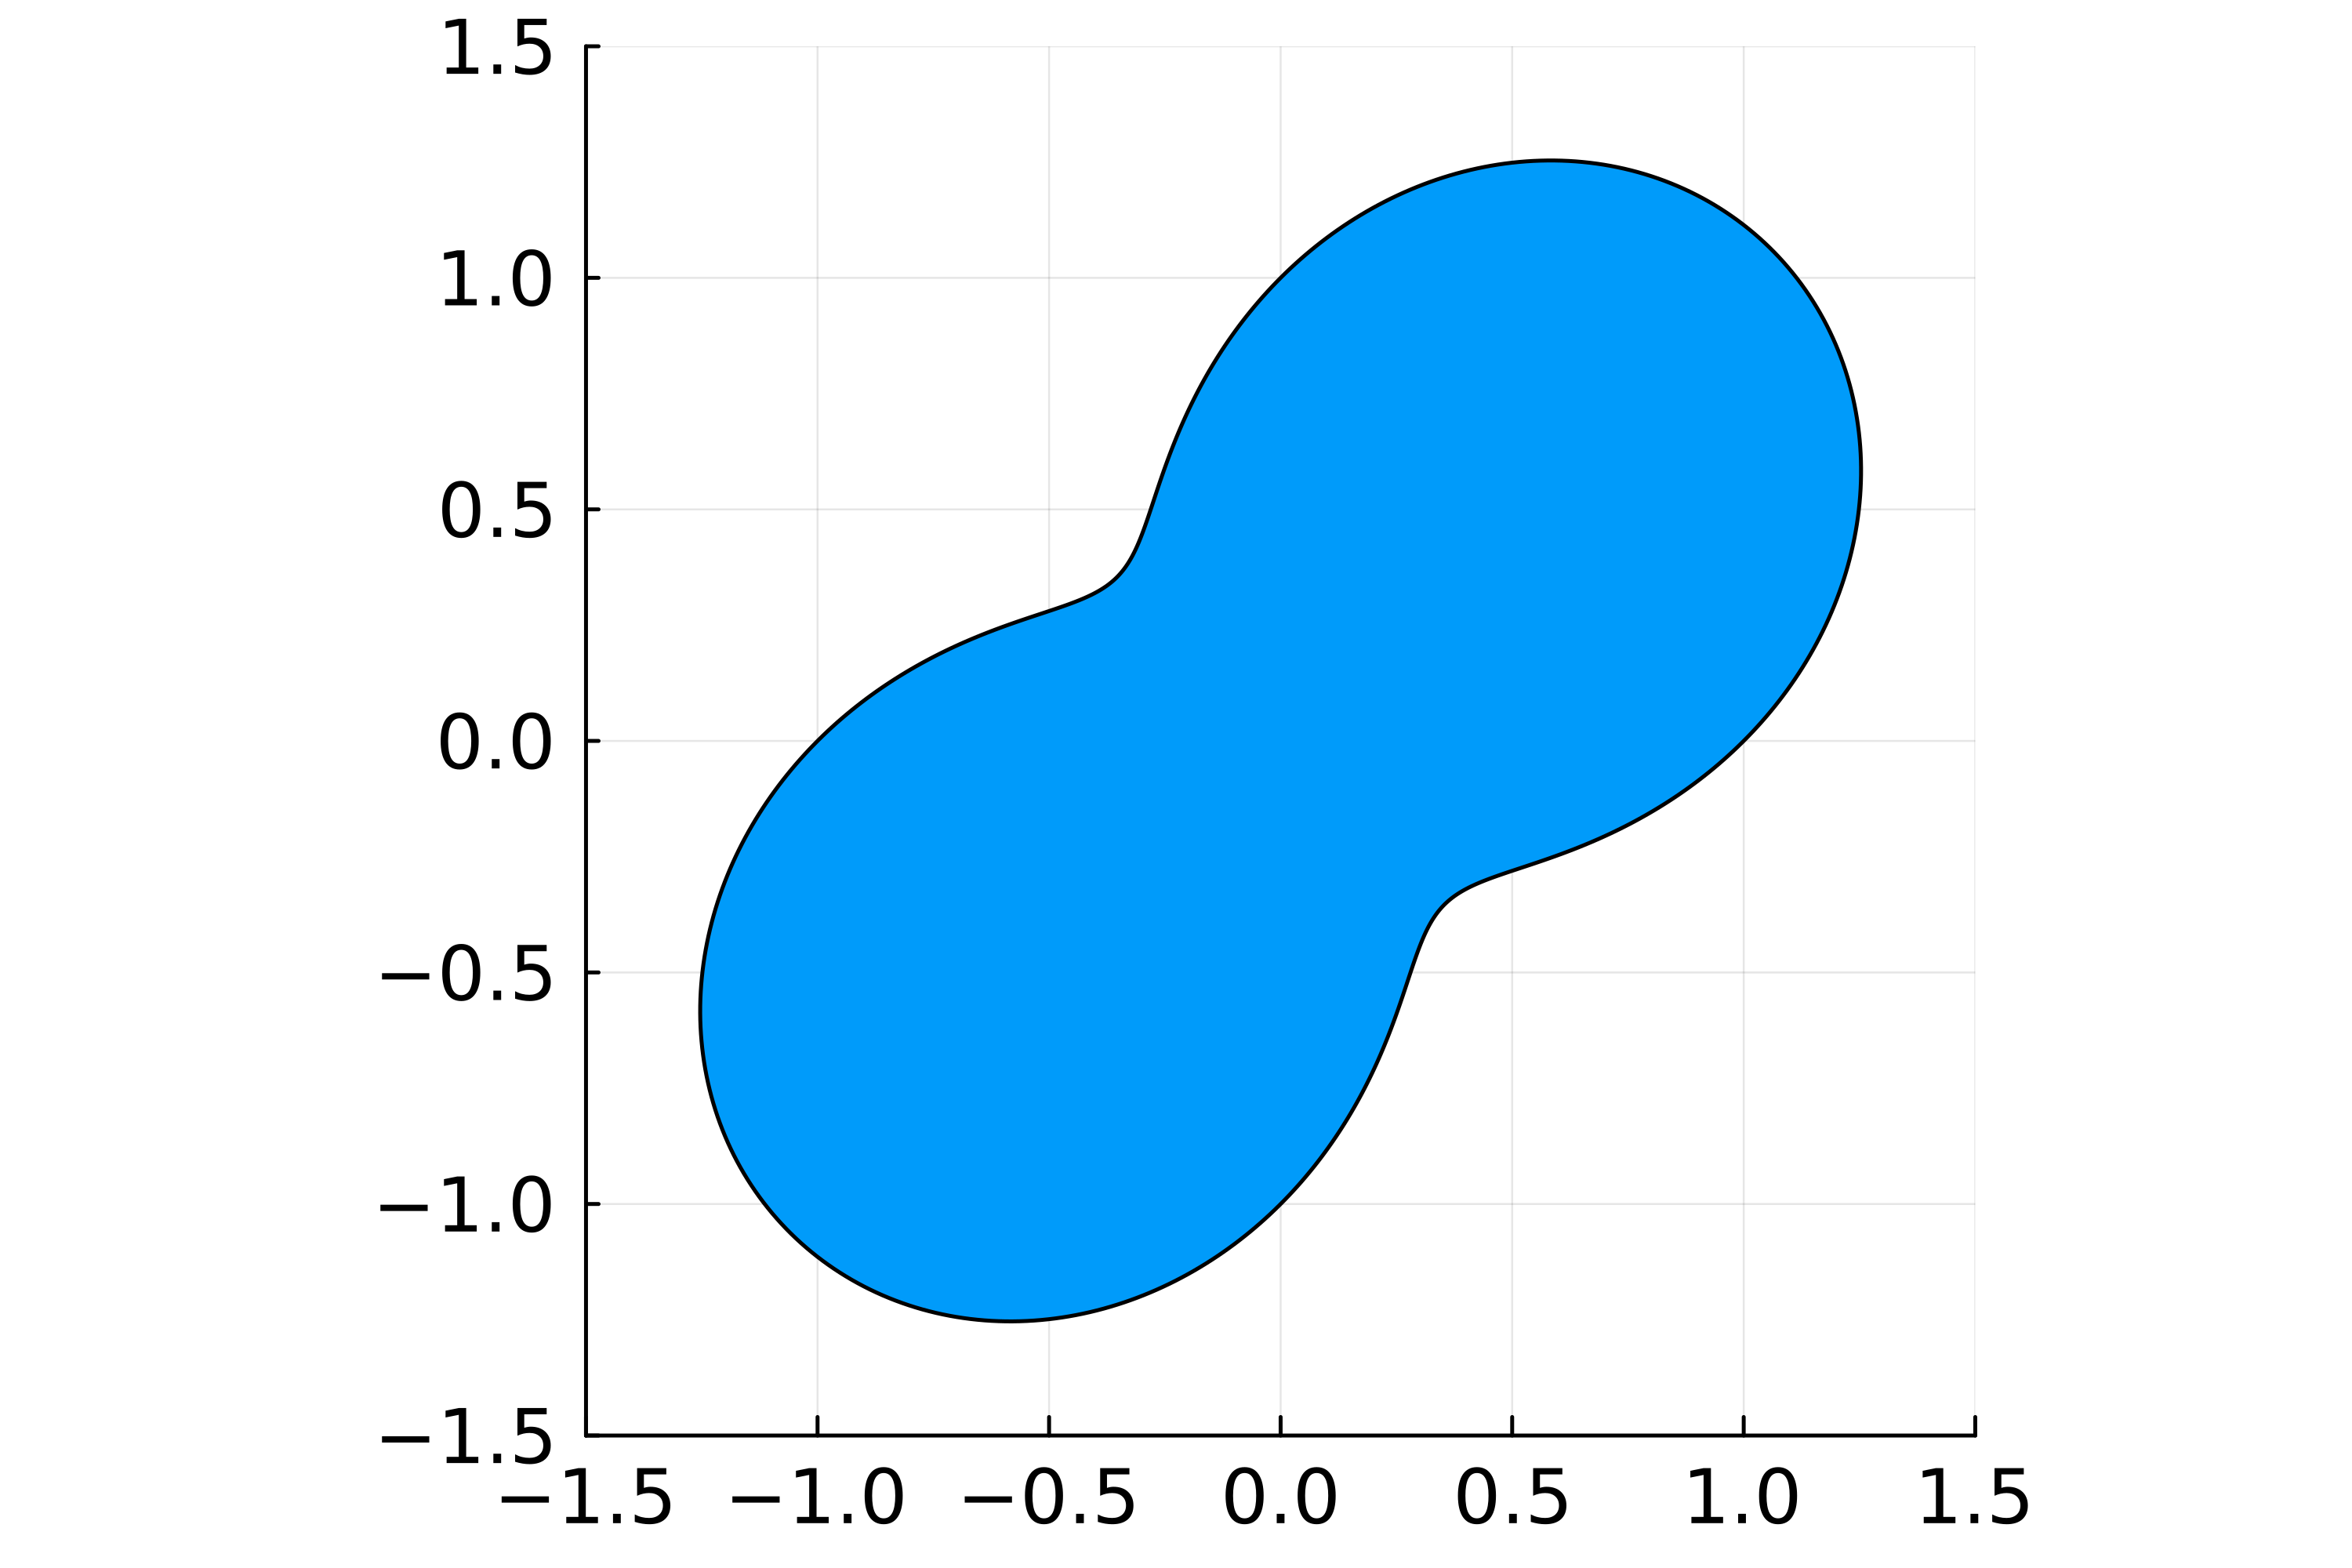
\includegraphics[width=\textwidth]{plotExample2_peanut.png}
		\caption{peanut shaped cell: \\ $r_{b}(\phi) = \frac{1}{2}\sin(2\phi) + 1$}
		\label{fig:peanut}
	\end{subfigure}
	\hfill
	\begin{subfigure}{0.3\textwidth}
		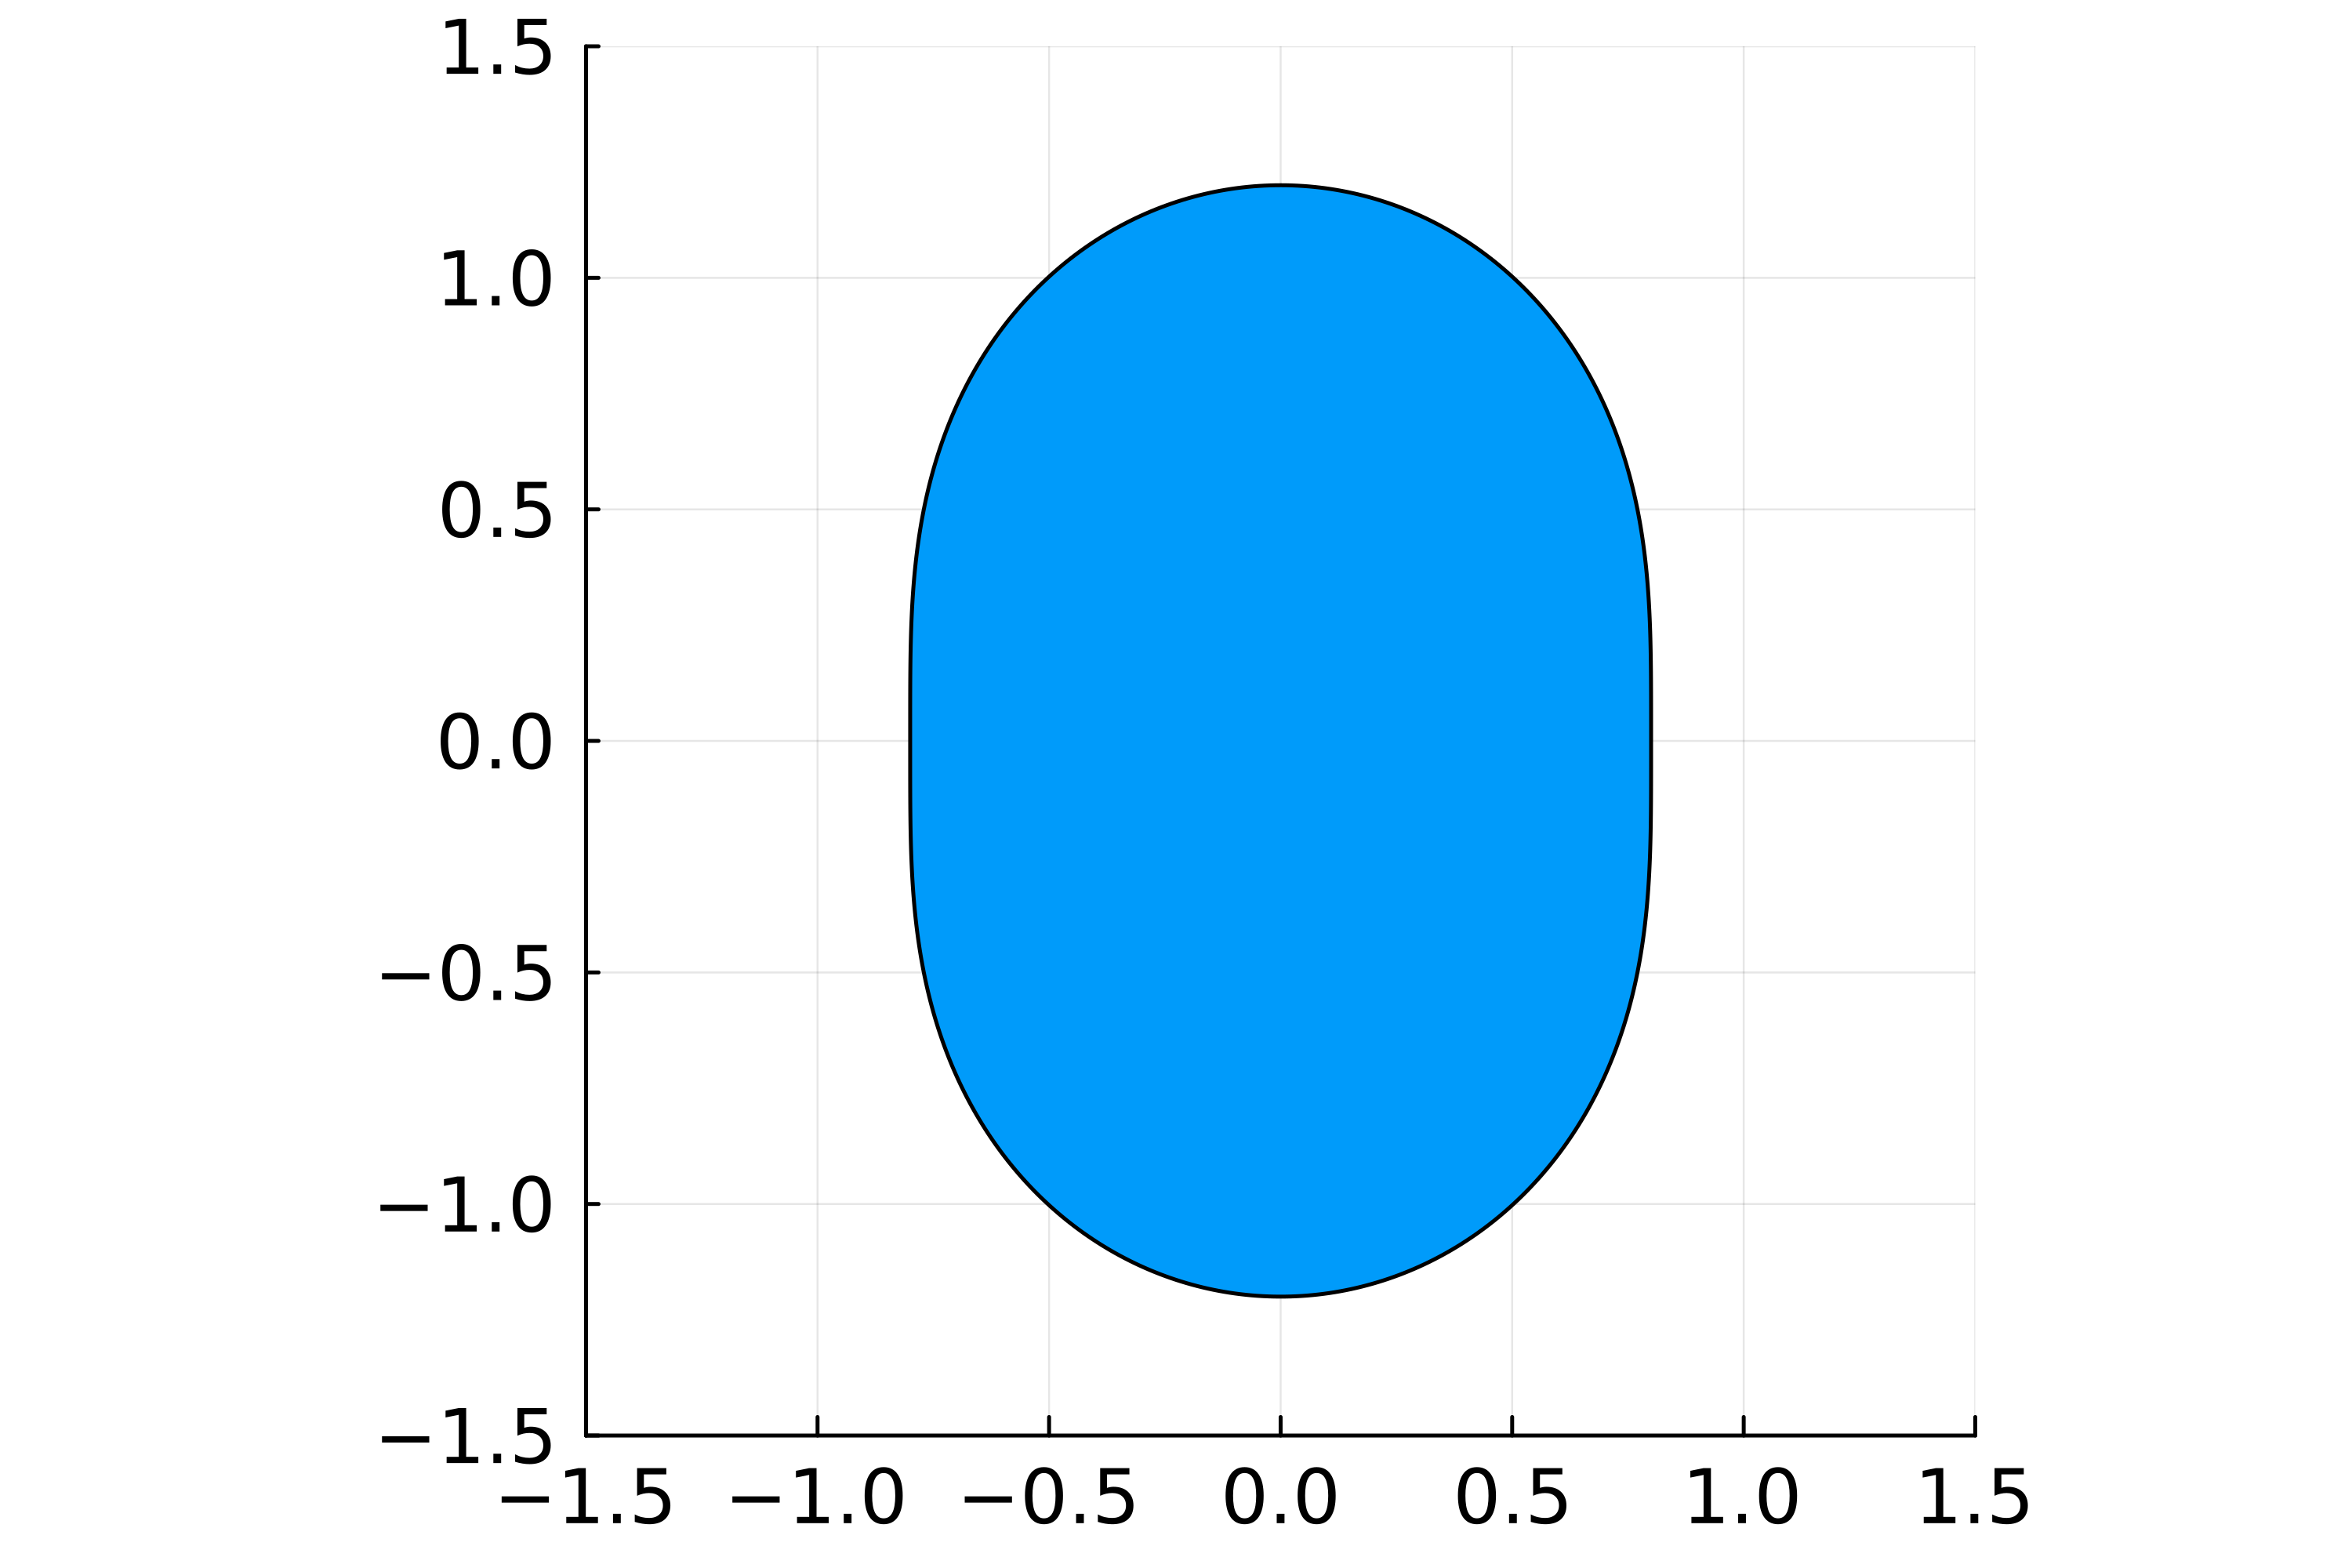
\includegraphics[width=\textwidth]{plotExample3_oval.png}
		\caption{oval cell: \\  $r_{c}(\phi) = 1 - \frac{1}{5}\cos(2\phi)$}
		\label{fig:oval}
	\end{subfigure}
	\caption{First examples of cell plots with centre $\vec{c} = (0,0)^T$.}
	\label{fig:plotExamples}
\end{figure}
\begin{definition} \textbf{Star domain}\\
	Any subset $S \subset \R^2 $ is star shaped if and only if there exists a point $\vec{c} \in S$ such that the connecting line from $\vec{c}$ to any other point $\vec{x} \in S$ is completely located in $S$. The point $\vec{c}$ is then called star centre. \\
\end{definition}
\begin{definition} \textbf{Convex domain}\\
	A domain $D \subset \R^2$ is said to be convex if for any two points $\vec{x}_1, \vec{x}_2 \in D$ their connection $\overline{\vec{x}_1 \: \vec{x}_2}$ lies entirely in $D$. \\ 
\end{definition}
\begin{definition} \textbf{Polygon} \\
	A polygon is a closed geometric figure in the two dimensional space $\R^2$, formed by connecting a finite number of straight line segments. It can be represented be a sequence $(\vec{x}_1, \ldots, \vec{x}_N)$ of its vertices. \\
	The following characteristic can be attributed to a polygon.
	\begin{enumerate}[(i)]
		\item A \textbf{simple} polygon is a polygon where no two line segments cross each other.
		\item A polygon has a \textbf{positive orientation} if the vertices are ordered counterclockwise.
		\item A polygon has a \textbf{negative orientation} if the vertices are ordered clockwise.
	\end{enumerate}
\end{definition}
An equivalent criterion for a polygon to be convex is that each interior angle is less than or equal to 180°. Every convex polygon is also star shaped. If a polygon $P$ is convex, one can even choose any point $\vec{x} \in P$ as the star centre. \\
\begin{definition} \textbf{Discrete form (DF)} \label{def:DF}  \\
	An ordered sequence of points $C = (\vec{x}_1, \ldots , \vec{x}_N)$ is considered to be a cell in its discrete form (DF) if the polygon that results when connecting every point with its neighbours and $\vec{x}_1$ with $\vec{x}_N$ is simple and positively orientated. \\	
	Cells in the DF model are sometimes just called discrete cells. \\
\end{definition}
\paragraph{Relationship between CRF and DF cells} \text{} \\
Having introduced the two Definitions \ref{def:CRF} and \ref{def:DF}, we will shortly give a comparison of these different cell models. \\ 
On one hand, the CRF model is able to describe not only an endless amount of vertices, like the DF model, but it can explain the whole cell wall as a continuous path. This is why we call the model continuous. Using the CRF model, one can compute arbitrary many vertices like portrayed in Figure \ref{fig:SketchCompWallPoint1}, enabling to plot the cells in a correspondingly high resolution. 
CRF cells always have some good properties. In a CRF $C = (\vec{c}, r)$ every angle around the centre has exactly one radius value what makes it impossible for the cell wall to cross itself. It is also not very hard to recognise that those cells are always star shaped with the star centre $\vec{c}$. \\
On the other hand, we have got the DF model. It is simpler than the first model, because it does not deliver the information of the whole cell wall, but only some wall points of it. Thus, we call this model discrete. The wall points are called vertices in this thesis, correlating to the paper \cite{Fletcher14} from the introduction. With a DF model, one can represent any simple polygon. This means that, as a rule, no further properties of these cells can be detected. \\ 
There are possibilities to compare cells from the different models.\\
\begin{definition} \textbf{Matching cells}\\
	A DF cell $\zeta$ and a CRF cell $C$ are called matching if all vertices in $\zeta$ are located on the cell wall described by $C$. \\
\end{definition}
DF cells that match a CRF cell inherit the property of being star shaped. \\
There are possibilities to switch from one model to the other. 
An example of switching from CRF to DF is the following. For $N \in \mathbb{N}$ angles 
\begin{center}
	$\phi_i = i \dfrac{2 \pi}{N}, \qquad 0 \leq i \leq N-1$, 
\end{center}
compute the according vertices $\vec{x}_1, \ldots, \vec{x}_N$ like in Figure \ref{fig:SketchCompWallPoint1} and save them in this order. \\
It is also possible to create a matching CRF out of a given DF if it is star shaped. To do so, one has to set $\vec{c}$ as a star centre of the DF cell. Afterwards, the radius function $r$ can be obtained through a smooth interpolation between the fixed radii $r_i = \norm[\vec{c} - \vec{x}_i]$ at the corresponding angles of rising $\phi_i$ between the line $\overline{\vec{c} \: \vec{x}_i}$ and the $x$ axis. In order to obtain a radius function fulfilling Definition \ref{def:CRF}, one must also consider the smoothness requirements at the interval ends of $[0, 2 \pi]$.  \\
Note, that the changeover from one model to another is never unique. For example, if one wants to derive a CF cell out of a CRF, there are different amounts $N$ of vertices possible. Or, if one wants to change the model from DF to CRF, there are different interpolations for $r$ possible. \\
It is important to understand that it is not possible to draw a one to one correspondence between two cells from the different models, because one can always convert a CRF cell to a DF cell ambiguously and vice versa. 

\subsection{Computation of area and overlap}
Next, we want to figure out how to calculate the area of such cells. Therefor we choose the now coming approach. Let us at first focus on cells in their CRF. In this subsection $C$ and $\zeta$ always represent CRF cells. 
If we had given the indicator function $\mathbbm{1}_{C}(\vec{x})$, that has the value $1$ if the point $\vec{x} \in \mathbb{R}^2$ lies within the cell $C \subset \mathbb{R}^2$ and $0$ otherwise, then we could obtain the cell area with the integral
\begin{center}
	$A_{C} = \int_{\mathbb{R}^2} \mathbbm{1}_{C}(\vec{x}) d\vec{x}$.
\end{center}
That is why we now construct a similar function with the information we get from the cell's CRF. First we take a look at the function 
\begin{center}
	$f(x) = \frac{1}{2}(1 + \tanh(s[1 - |x|]))$,
\end{center}
\begin{figure}[h!]
	\centering
	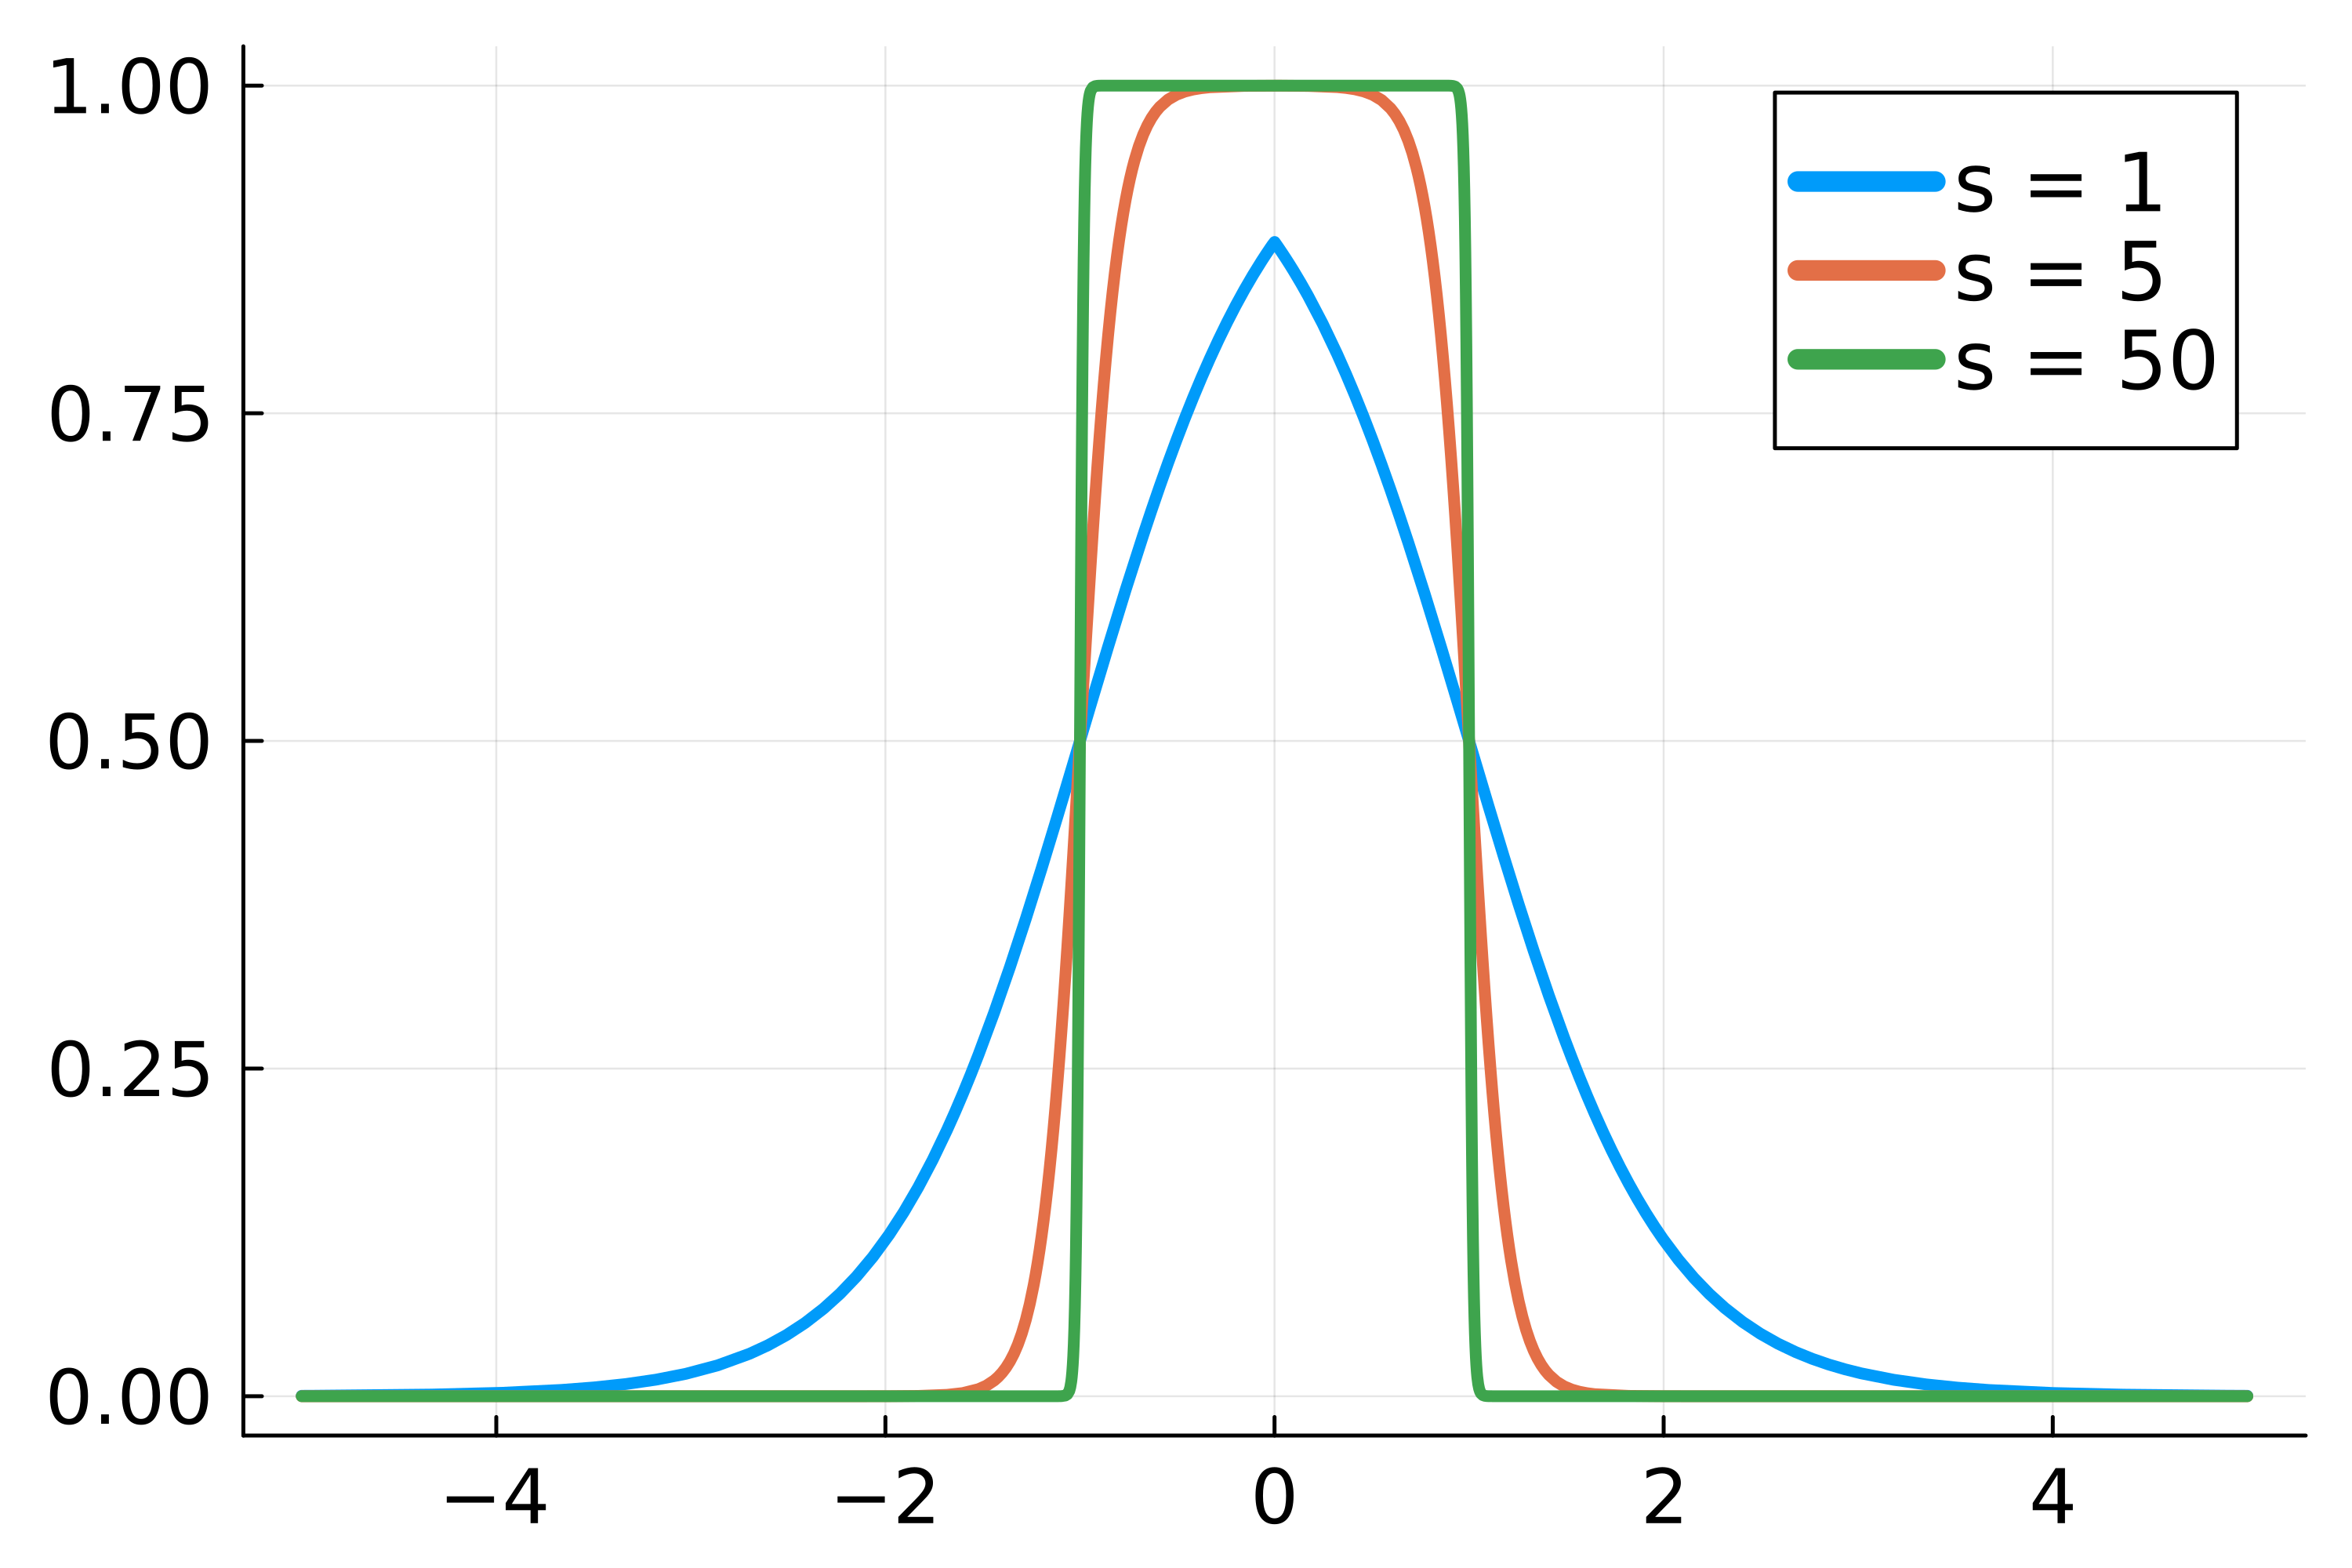
\includegraphics[width=8cm]{preSmoothIndicator.png}
	\caption{Different plots of $f(x)$ for $s = 1$ (blue), $s = 5$ (orange) and $s = 50$ (green). The $x$ axis denotes the value of the argument $x$, while the $y$ axis denotes the value of $f$ at that point. }
	\label{fig:pre_smooth_indicator}
\end{figure}

with a positive number $s \in \mathbb{R}_{>0}$.
As we can see in Figure \ref{fig:pre_smooth_indicator}, the larger we choose $s$, the more this function looks like $\mathbbm{1}_{[-1,1]}$. \\
For large $s$, $f$ is nearly $1$ if the term in the hyperbolic tangent is positive and nearly $0$ otherwise. Hence, we set our $s \gg 1$ and choose a different term inside of the hyperbolic tangent which is positive if and only if $\vec{x} \in C$. The following computation will give us such a term. Let $\phi_{\vec{x}}$ be the angle of rise of the line segment that connects the centre $\vec{c}$ with $\vec{x}$ in respect to the $x$ axis. The angle of rising can also be computed using the trigonometric functions. \\
Then, we can observe that a point $\vec{x} \in \R^2$ is in $C$ if and only if 
\begin{center}
	$r(\phi_{\vec{x}}) \geqslant \norm[\vec{c} - \vec{x}]$,
\end{center}
what is equivalent to
\begin{center}
	$r(\phi_{\vec{x}}) - \norm[\vec{c} - \vec{x}] \geqslant 0$. 
\end{center}
Thus, we establish our indicator comparable function, that we will call $\psi$, like this. \\
\begin{definition} \textbf{Smooth indicator function} \label{def:smoothIndicator}\\
	For a cell $C = (\vec{c}, r)$ given in its CRF, we declare the smooth indicator function to be 
	\begin{center}
		$\psi_C: \mathbb{R}^2 \rightarrow (0,1)$, $\vec{x} \mapsto \frac{1}{2}(1 + \tanh(s[ r(\phi_{\vec{x}}) - \norm[\vec{c} - \vec{x}]]))$, 
	\end{center}
	where $\phi_{\vec{x}}$ is the angle of rise of the line segment that connects the centre $\vec{c}$ with $\vec{x}$ in respect to the $x$ axis. The scaling factor $s \gg 1$ determines how rapid the transition from inside and outside of the cell is if one draws the analogy to the normal indicator function.\\
\end{definition}
\begin{figure}[t!]
	\centering
	\begin{subfigure}{0.4\textwidth}
		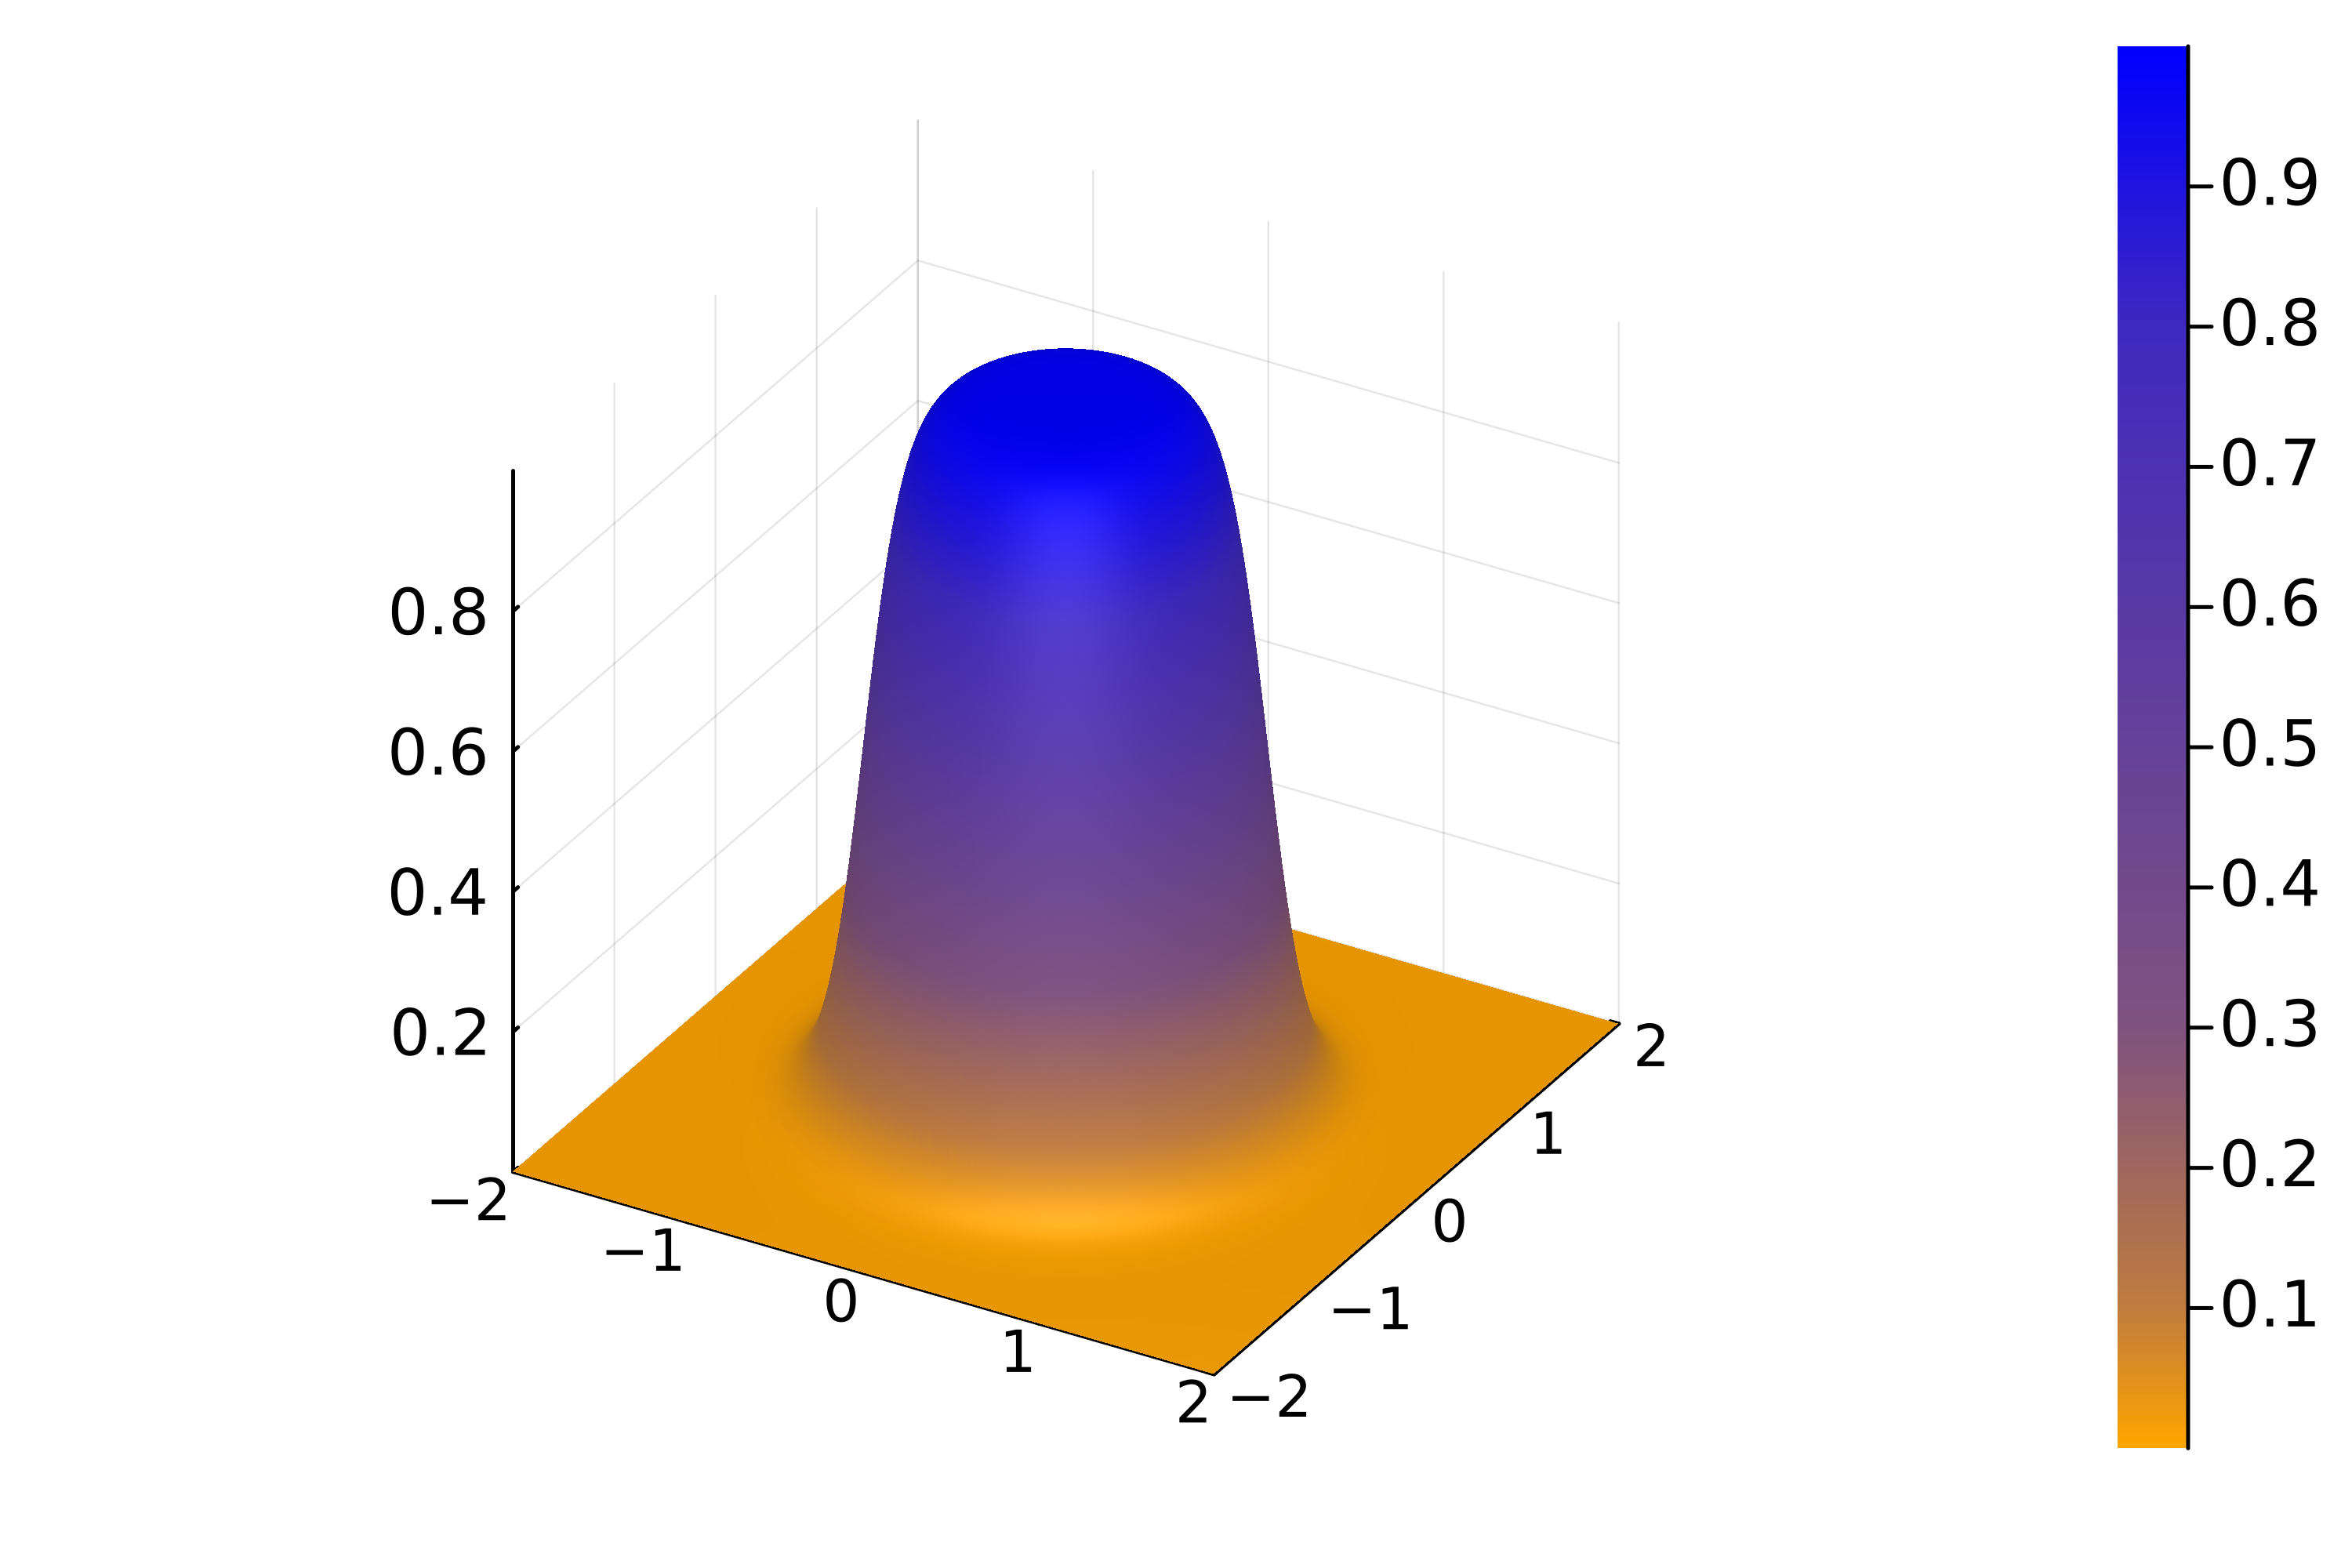
\includegraphics[width=\textwidth]{psi_func/psi_function_plot_s=5.png}
		\caption{$\psi_{unit\:circle}$, $s=5$}
	\end{subfigure}
	\hfill
	\begin{subfigure}{0.4\textwidth}
		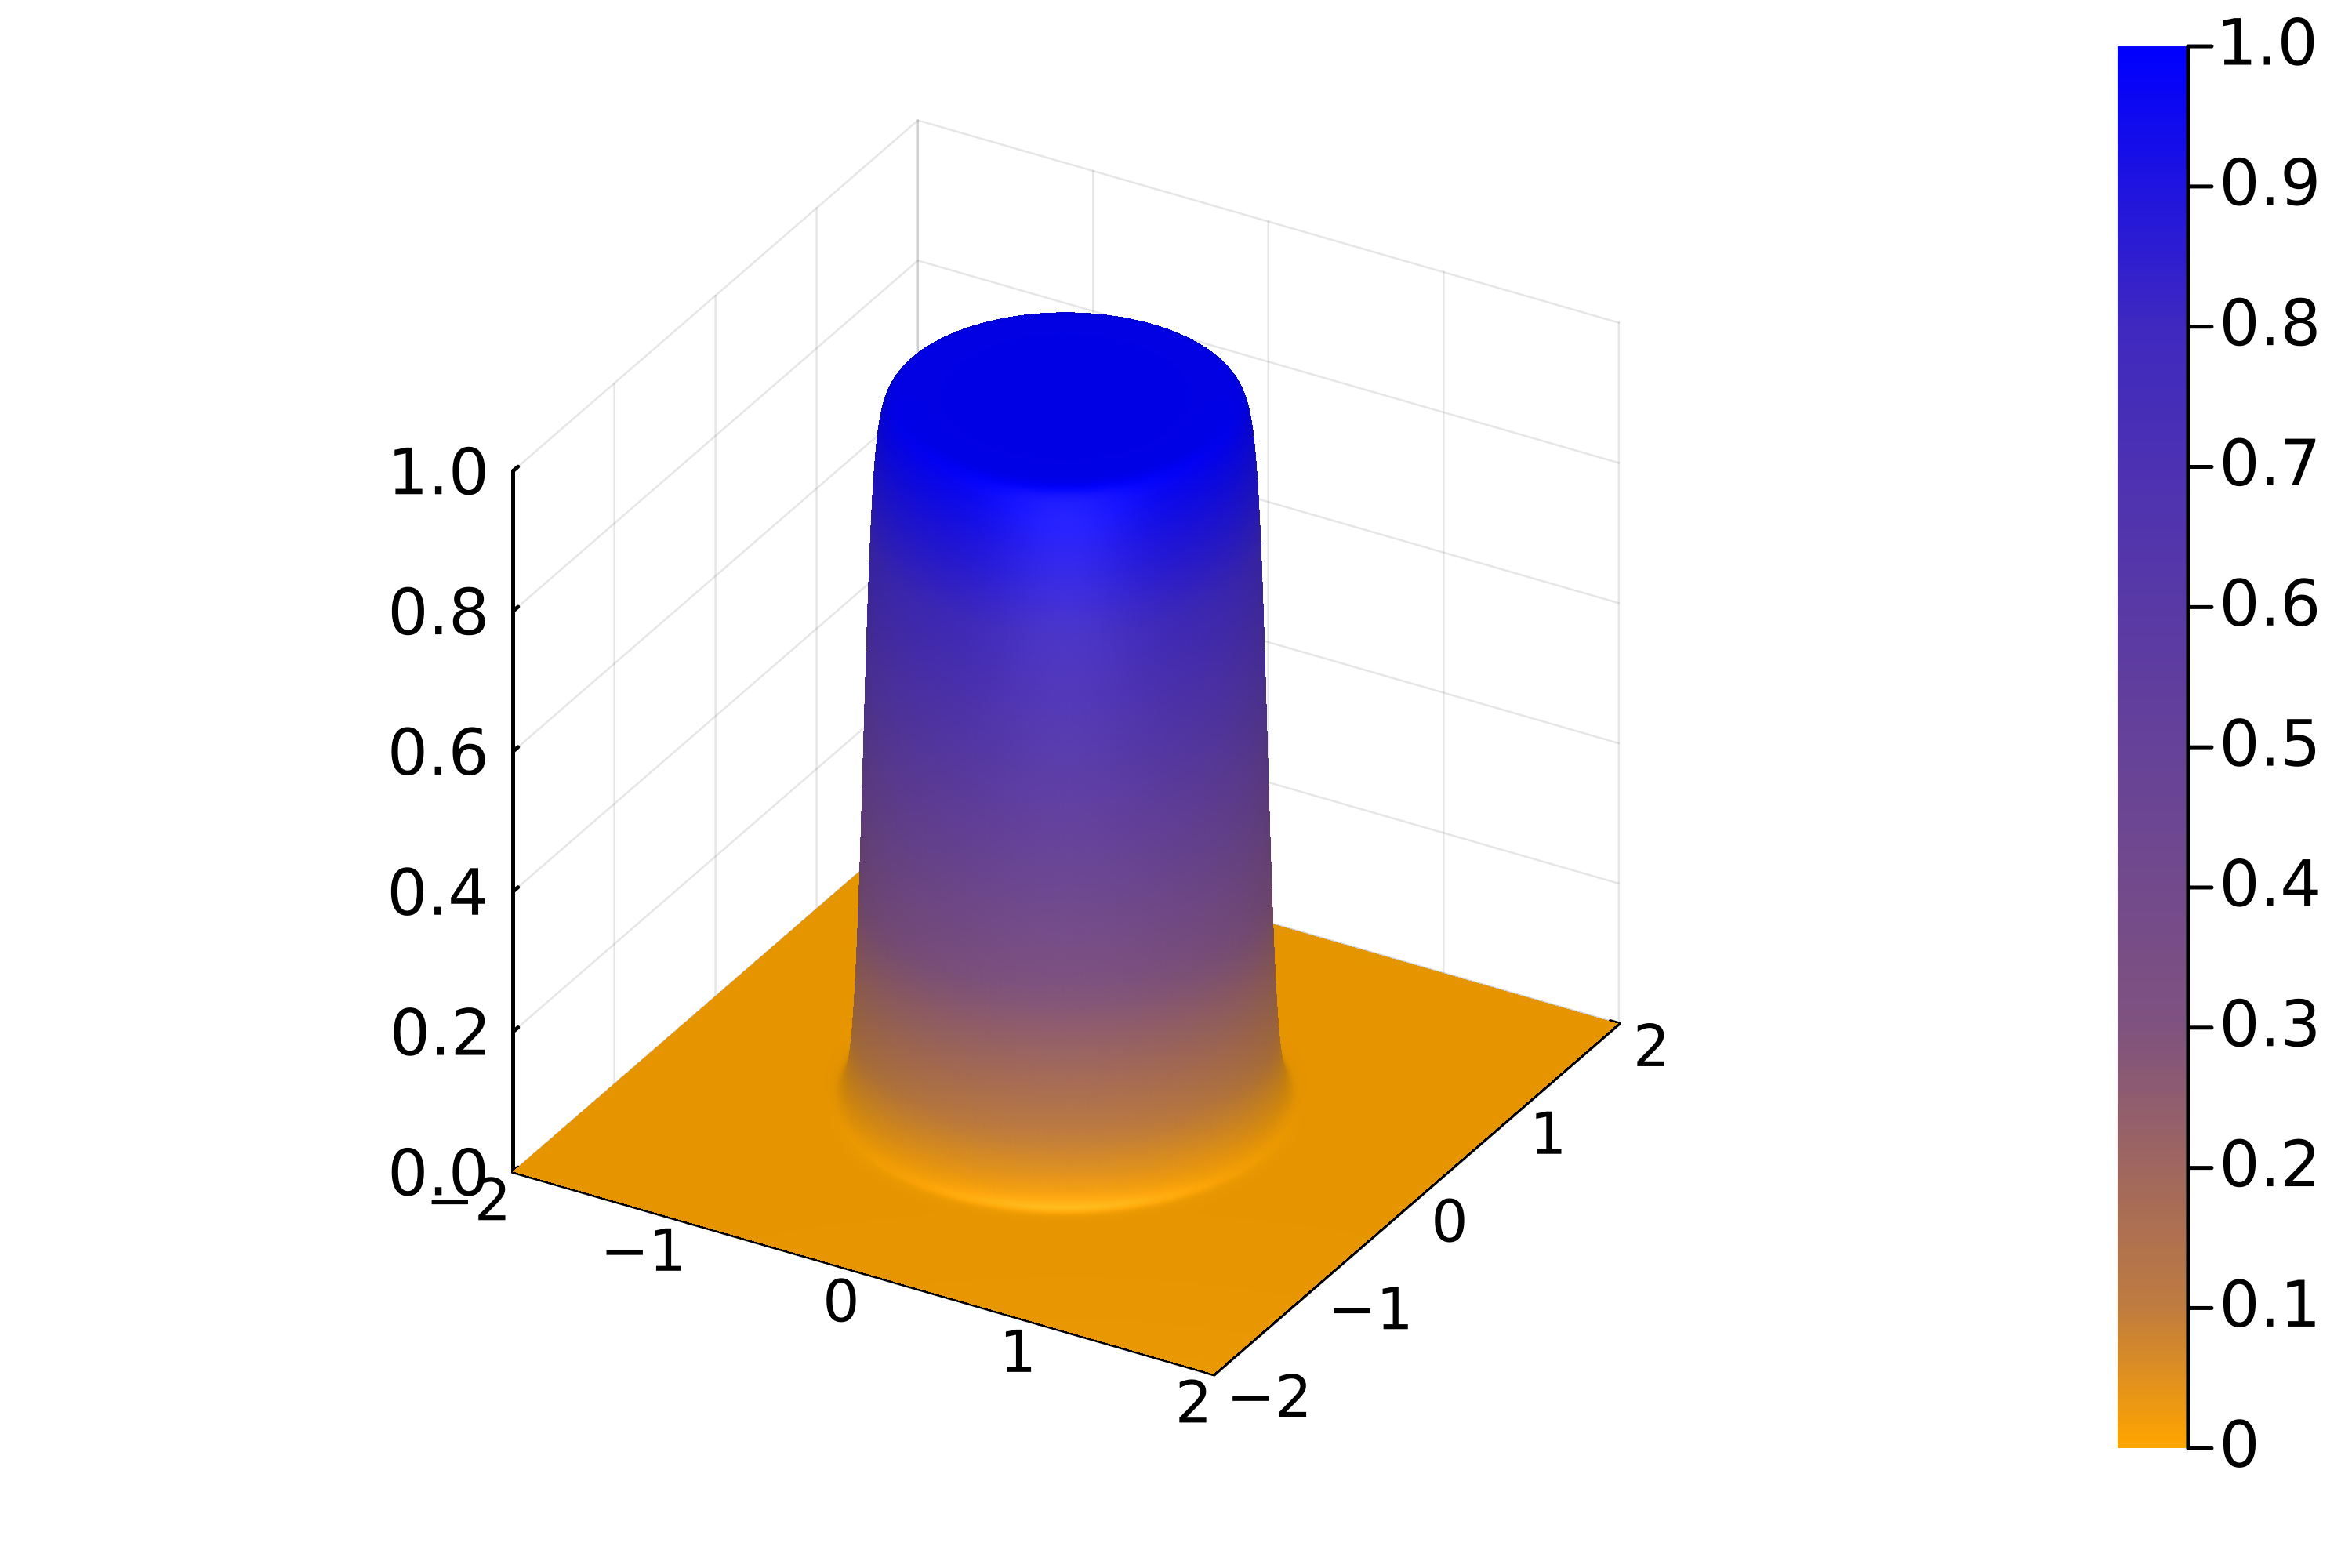
\includegraphics[width=\textwidth]{psi_func/psi_function_plot_s=20.png}
		\caption{$\psi_{unit\:circle}$, $s=20$}
	\end{subfigure}
	\hfill
	\begin{subfigure}{0.4\textwidth}
		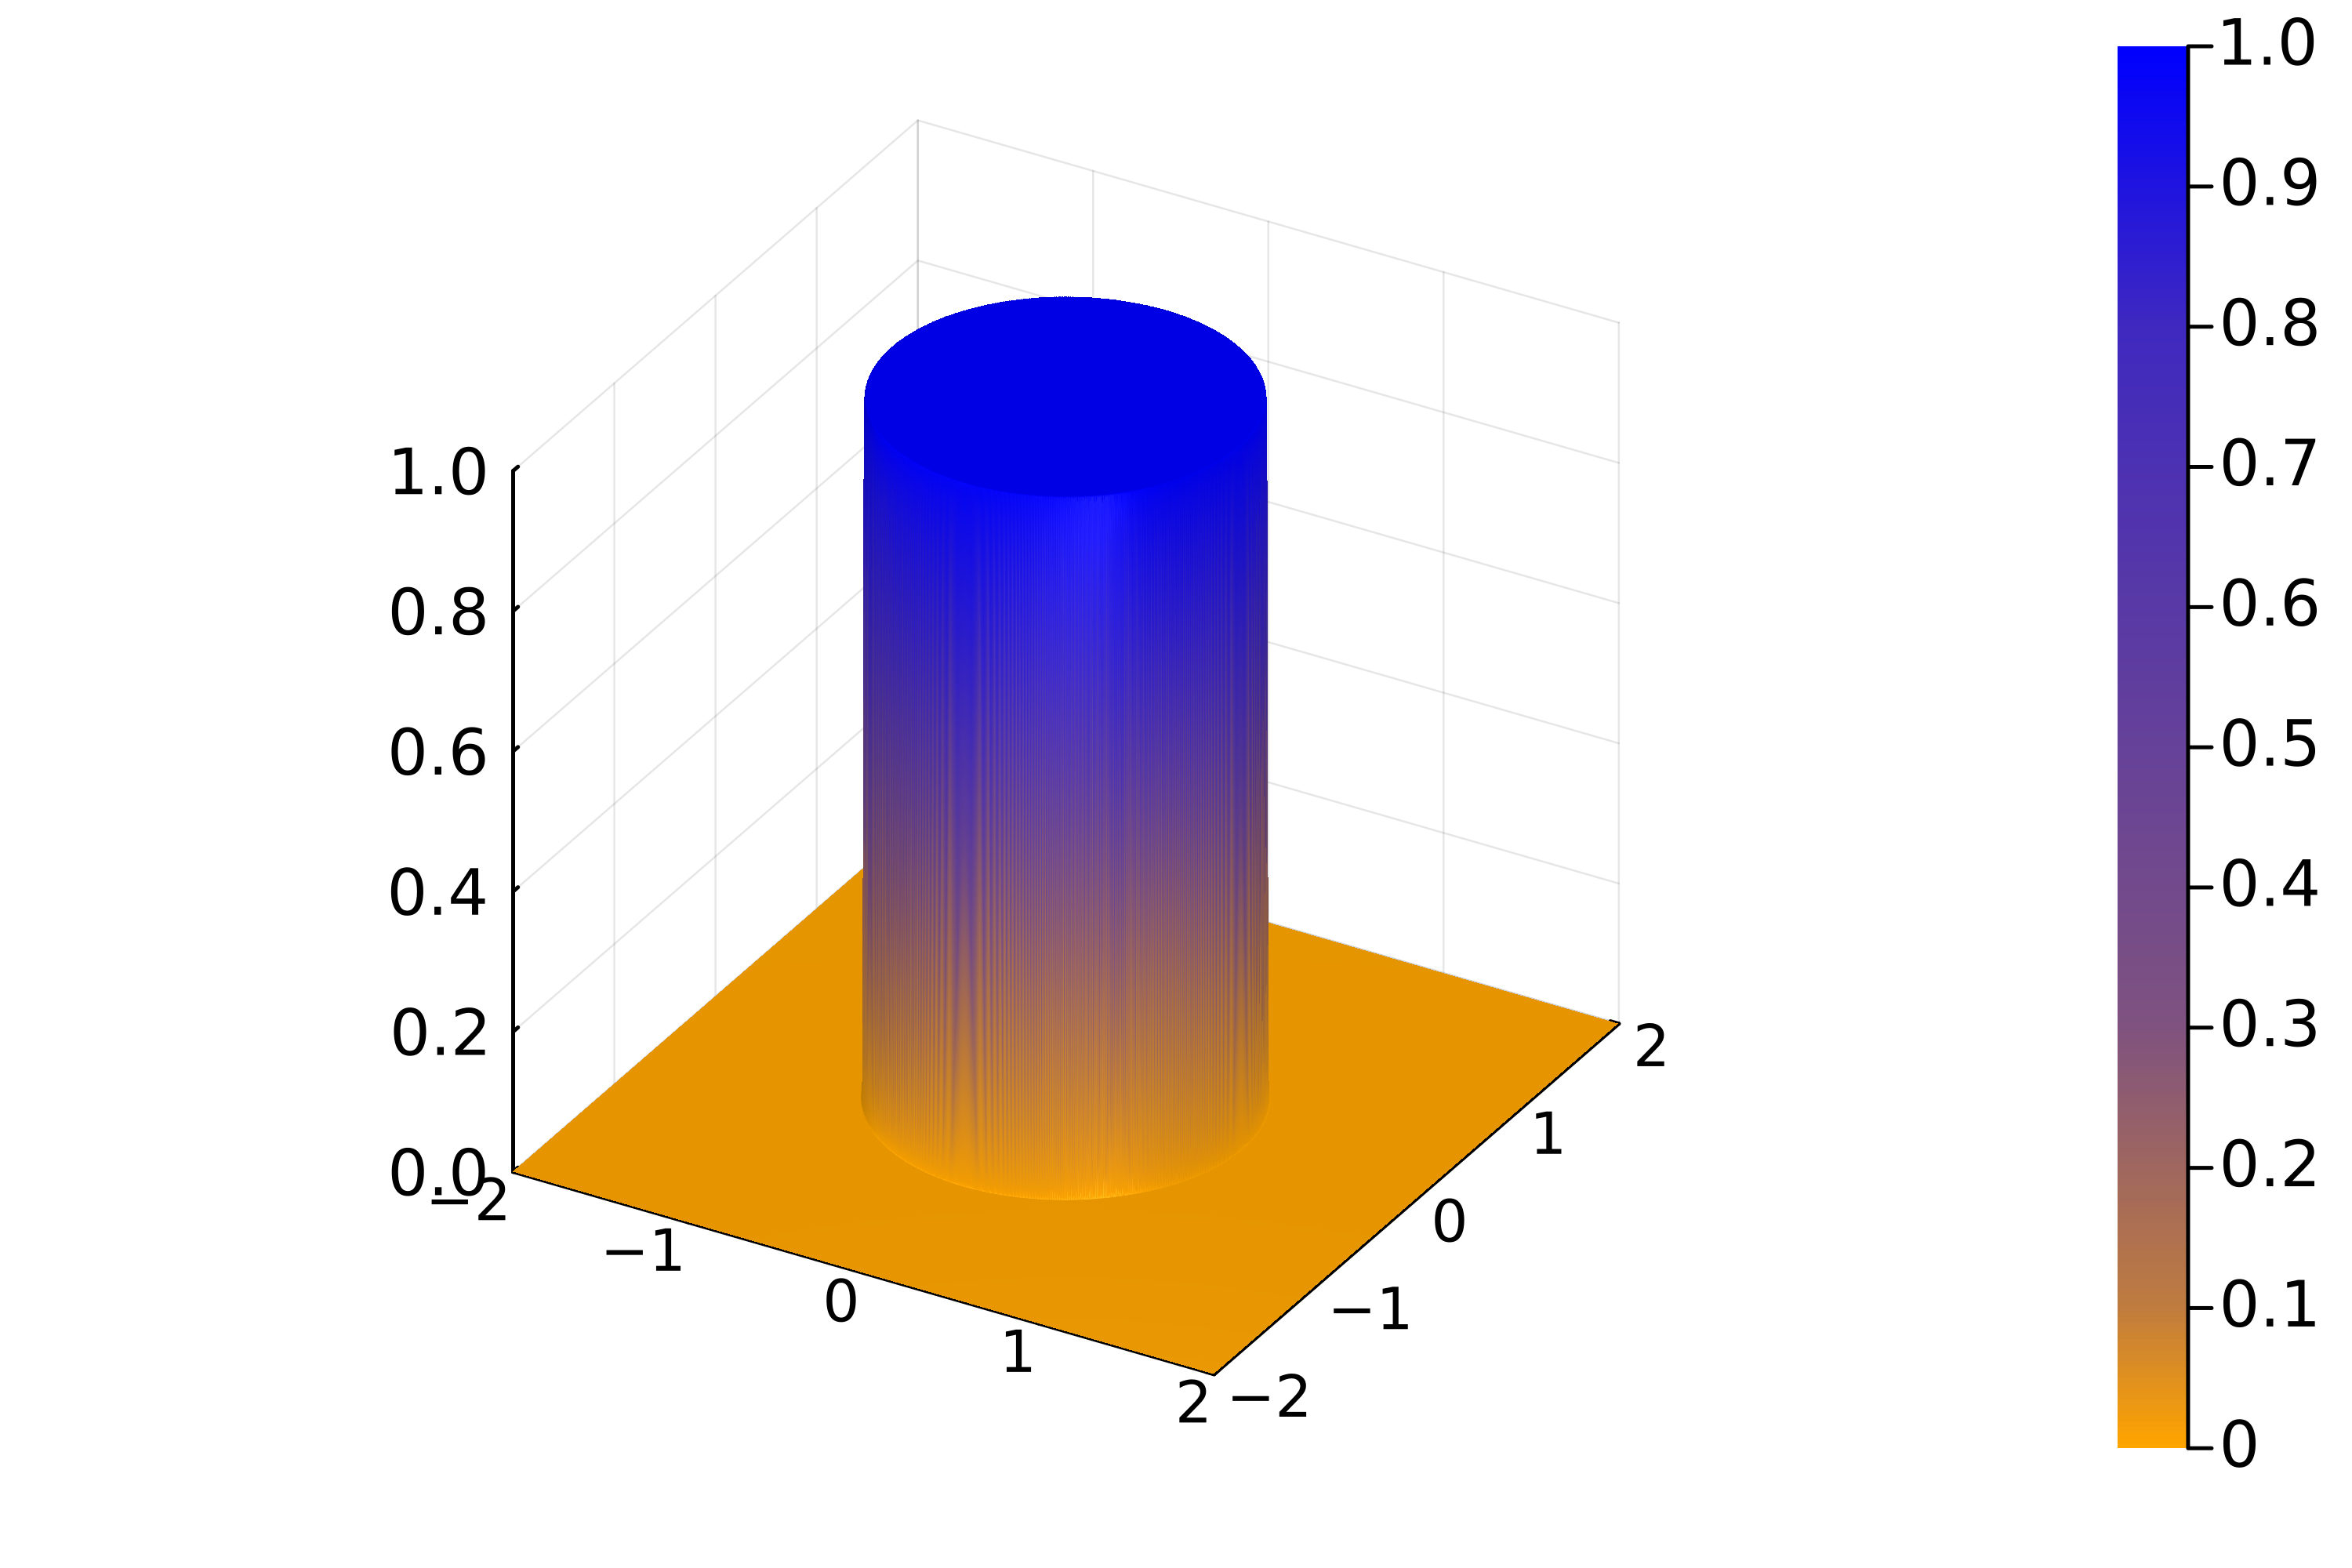
\includegraphics[width=\textwidth]{psi_func/psi_function_plot_s=500.png}
		\caption{$\psi_{unit\:circle}$, $s=500$}
	\end{subfigure}\hfill
	\begin{subfigure}{0.4\textwidth}
		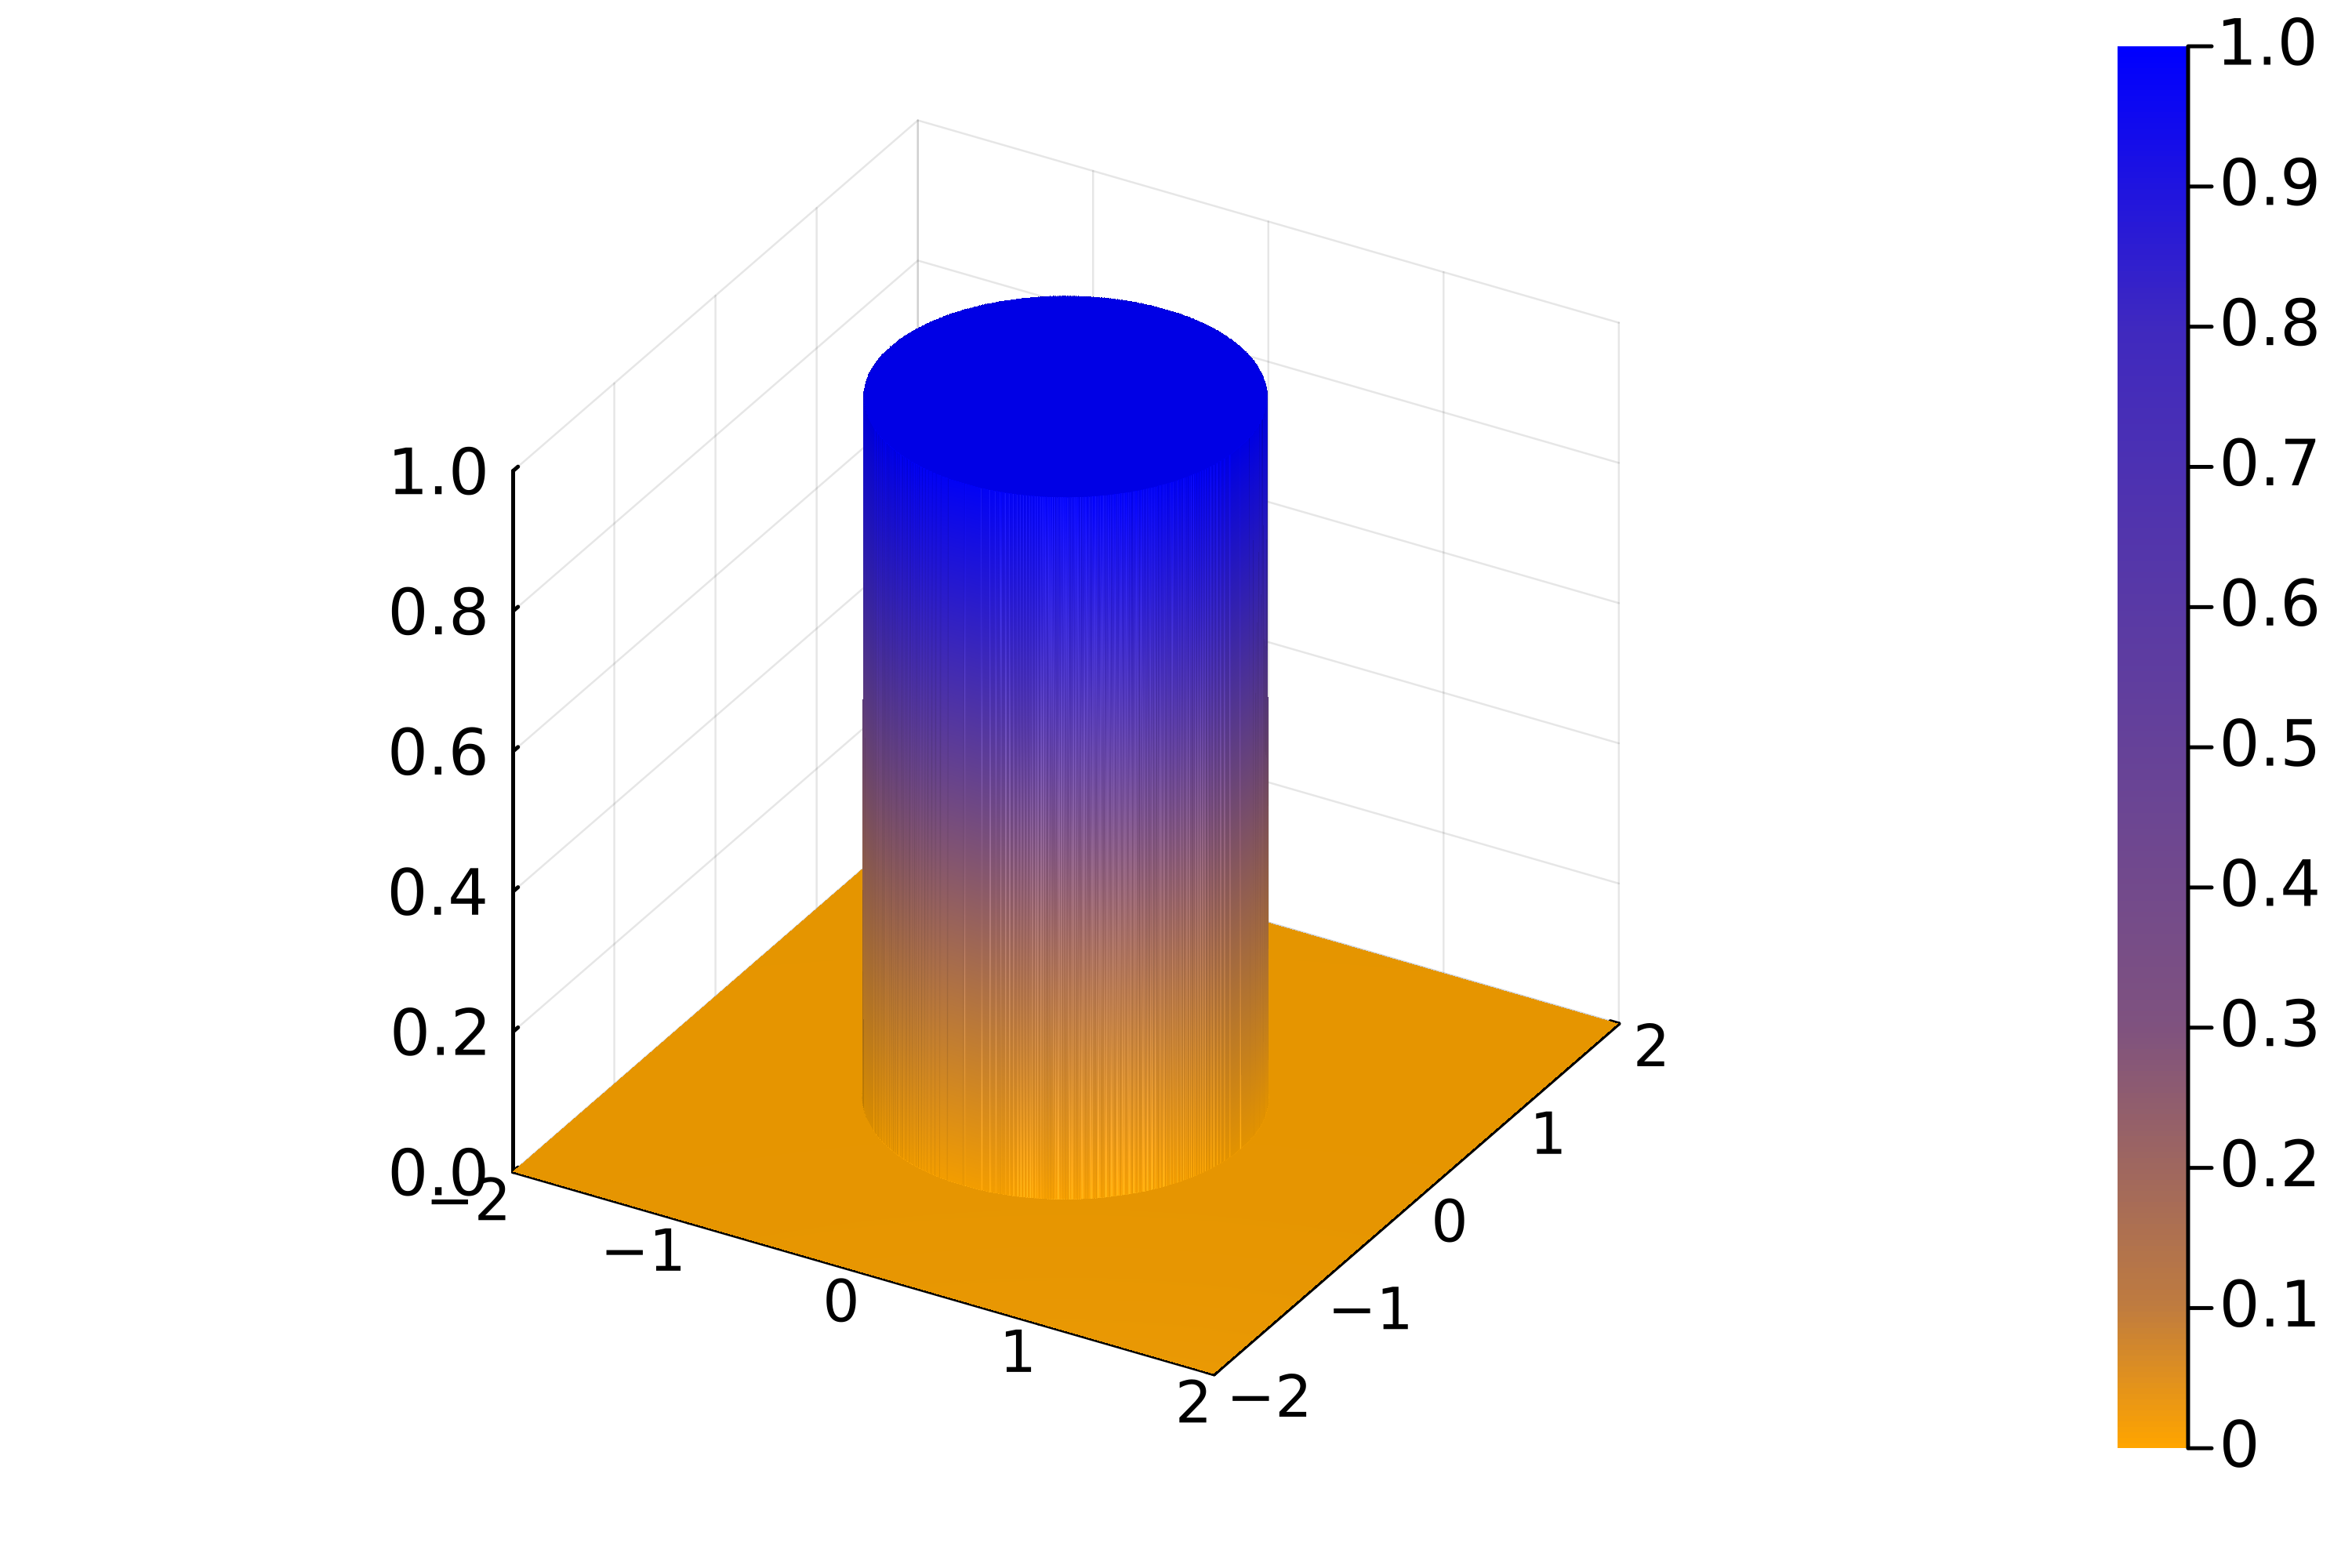
\includegraphics[width=\textwidth]{psi_func/indicator_func_unitcircle.png}
		\caption{real indicator $\mathbbm{1}_{unit\:circle}$}
	\end{subfigure}
	\caption{Plots of $\psi_{unit\:circle}$ with different $s \in \{5, 50, 500\}$ in comparison with the normal indicator function of the unit circle.}
	\label{fig:psi_plot}
\end{figure}
If we take a look at the cell $((0,0)^T, \phi \mapsto 1)$ that is represented by the unit circle, we obtain
\begin{center}
	$\psi_{unit\:circle}(\vec{x}) = \frac{1}{2}(1 + \tanh(s[ 1 - \norm[\vec{x}]]))$.
\end{center}
Right down to the radius function of the cell, every other function that is composed in $\psi$ is infinitely differentiable. That is why the smooth indicator function has the same smoothness as $r$. \\
In Figure \ref{fig:psi_plot} we get to see plots of $\psi_{unit\:circle}$ for different $s$ and the indicator function $\mathbbm{1}_{unit\:circle}$. As expected, the larger we choose $s$, the steeper the slope gets and the closer $\psi_{unit\:circle}$ gets to $\mathbbm{1}_{unit\:circle}$. For smaller $s$ the product $\psi_{C} \psi_{\zeta}$ can be greater than zero in areas near both cells $C$ and $\zeta$ where they actually do not meet. This could be used to add neighbouring cell interaction, although these cells are not yet overlapping. \\
As mentioned before, we can now use the smooth indicator function to compute the area of a cell as we calculate the integral
\begin{center}
	$A_{C} = \int_{\mathbb{R}^2} \mathbbm{1}_C(\vec{x}) d\vec{x} \approx \int_{\mathbb{R}^2} \psi_C(\vec{x}) d\vec{x} = \frac{1}{2} \int_{\mathbb{R}^2} (1 + \tanh(s[ r(\phi_{\vec{x}}) - \norm[c - \vec{x}]])) d\vec{x}$.	
\end{center}
With these smooth indicator functions, we are also able to compute the overlap of different cells. We just have to draw the analogy to the standard indicator function once more to see 
\begin{center}
	$A_{C \cap \zeta} = \int_{\mathbb{R}^2} \mathbbm{1}_{C \cap \zeta}(\vec{x}) d\vec{x} = \int_{\mathbb{R}^2} \mathbbm{1}_{C}(\vec{x})\mathbbm{1}_{\zeta}(\vec{x}) d\vec{x} \approx \int_{\mathbb{R}^2} \psi_{C}(\vec{x})\psi_{\zeta}(\vec{x}) d\vec{x}$.	
\end{center}
Thus, we just have to multiply the smooth indicator functions of all cells that we want to determine the overlap from. The final numerical implementation and its properties will be discussed in the next paragraph. \\
For now, we want to take a look at the area calculation of the discrete model. Fortunately, there exists a direct formula for the area of simple polygons. \\
\begin{proposition}  \textbf{Shoelace formula for DF cells} \label{prop:Shoelace}\\ 
	Let $C = (\vec{x}_1, \ldots, \vec{x}_N)$ be a positively orientated DF cell with $\vec{x}_i = (x_i, y_i)^T$.
	Then, the area $A_C$ of $C$ can be determined through the shoelace formula
	\begin{center}
		$A_C = \frac{1}{2}\sum\limits_{i = 1}^{N} (x_i y_{i+1} - x_{i+1} y_i)$,
	\end{center} 
	where $\vec{x}_{N + 1} := \vec{x}_1$. \\
	Proof. 	\\
	An illustration of the proof is given in Figure \ref{fig:shoelace}, which is where the idea of the proof comes from. We can assume without the loss of generality that all coordinates are positive. Otherwise we could move the figure in the positive coordinate directions until all entries are positive without changing the area. \\
	For every $1 \leq i \leq N$ the edge $\overline{ \vec{x}_i \: \vec{x}_{i+1}}$ gets assigned to the area $T_i$ of the trapeze that arises when one connects the line segment vertically with the $x$ axis. We get
	\begin{center}
		$T_i = \frac{1}{2} (y_i + y_{i+1})(x_i - x_{i+1})$.
	\end{center}
	Keep in mind that $\vec{x}_{N + 1} := \vec{x}_1$. \\
	The area $T_i$ has a positive sign if $x_i \geq x_{i+1}$ (green arrow in Figure \ref{fig:shoelace}) and a negative sign otherwise (red arrow). As one can see in the figure, the negatively signed $T_i$'s take up exactly the areas that are superfluous if one just adds all the positive $T_i$'s. 
	Thus the total polygon's area is equal to the sum of all trapezes
	\begin{center}
		$A_C = \sum\limits_{i = 1}^{N} T_i = \frac{1}{2} \sum\limits_{i = 1}^{N} (y_i + y_{i+1})(x_i - x_{i+1}) = \frac{1}{2}\sum\limits_{i = 1}^{N} (x_i y_{i+1} - x_{i+1} y_i) $.
	\end{center} 
	\begin{figure}[h!]
		\begin{center}
			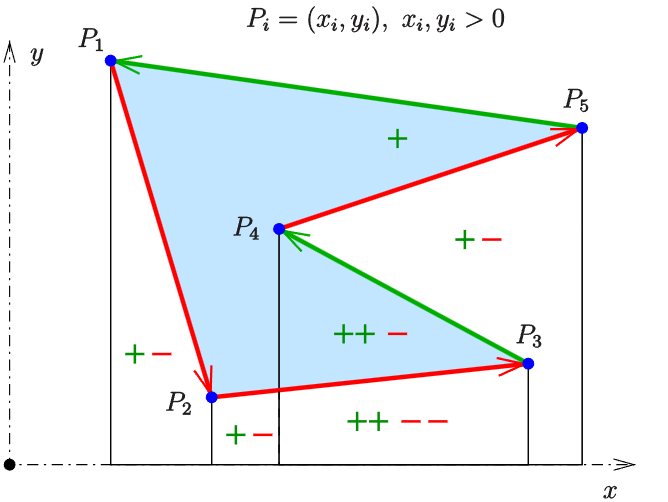
\includegraphics[width=8cm]{shoelace.png}
			\caption{
				This figure shows a geometrical interpretation of the shoelace formula. In difference to the proposition, here the vertices are called $P_i$ and not $\vec{x}_i$. \\
				Source: \cite{ShoelaceFigure2022}}
			\label{fig:shoelace}
		\end{center}
	\end{figure}
	\qed
\end{proposition}
This method is sometimes also called Gauss's area formula. A derivation of the formula can be found in \cite{Shoelace2014}. \\
Thus, we have got a quiet easy but powerful way to obtain the area of a single discrete cell. In order to evaluate the overlap of two discrete cells, we have to determine new cells which exactly cover the overlapping area. Once these cells are computed, it is no problem to compute the overlapping area by just using the shoelace formula on them. How to do that will be answered in the consecutive paragraph.

\subsection{Numerical approximation for the continuous area computation}
Until now, we have discussed ways to find out cell areas and overlaps of different cells of both the continuous and discrete model. \\
For the continuous case, where we have got the cells in their CRF, we introduced the smooth indicator function which delivers the cell area via the integral 
\begin{center}
	$A_{C} \approx \int_{\mathbb{R}^2} \psi_C(\vec{x}) d\vec{x} = \frac{1}{2} \int_{\mathbb{R}^2} (1 + \tanh(s[ r(\phi_{\vec{x}}) - \norm[c - \vec{x}]])) d\vec{x}$.
\end{center}
As this integral is really hard to solve explicitly, we rather want to solve it with a numerical method that we will now derive.\\ 
First of all, we need to find a domain over which we will integrate. It makes sense to choose a rectangle so that we can create a grid over it without much effort. 
Therefor, we iterate over the interval $[0, 2\pi)$ and compute the cell vertices at many angles with small constant shifts to find the coordinates $x_0, x_M, y_0, y_N$ that represent the $x$ coordinates most left and right and the $y$ coordinates most up and down. The rectangle $R = [x_0, x_M ] \times [y_0, y_N]$ will now cover the whole cell quite accurately.
Further on, we have to choose the amounts $M, N \in \N$ that will represent how many times we divide the sides of the rectangle, to obtain the mesh 
\begin{center}
	$h_x := \dfrac{x_M - x_0}{M}, \qquad h_y := \dfrac{y_N - y_0}{N}$, \\
	\smallskip
	$x_i := x_0 + i h_x, \qquad 0 \leq i \leq M$,\\
	\smallskip
	$y_j := y_0 + j h_y, \qquad 0 \leq j \leq N$.\\
\end{center}
Every point $(x_i, y_j)^T$ is a grid point of our mesh. 
We also need the midpoints of each sub rectangle which are given by the term
\begin{center}
	$\vec{m}_{i,j} := \begin{pmatrix} x_0 \\ y_0 \end{pmatrix}  + \begin{pmatrix} i h_x \\ j h_y \end{pmatrix} - \dfrac{1}{2} \begin{pmatrix} h_x \\ h_y \end{pmatrix}, \qquad  1 \leq i \leq M, \; 1 \leq j \leq N$,
\end{center}
for our numerical approximation.
With these preparations we are now ready to use the summed up midpoint rule.\\
\begin{proposition} \textbf{Summed up midpoint rule} \label{prop:summedMidpointRule}\\
	Let $f: R \rightarrow \mathbb{R}$ be a function that is integrable over a rectangular domain $R \subset \R^2$. For given increments $h_x$, $h_y$ and midpoints $\vec{m}_{i,j}$ like above, we can approximate the integral of f over R by the formula
	\begin{center}
		$\int_{R} f(\vec{x}) d\vec{x} \approx h_x h_y \sum\limits_{i=1}^{M} \sum\limits_{j=1}^{N} f(\vec{m}_{i,j}) =: Q_{N,M}^R(f)$. \\
	\end{center} 
\end{proposition}
Although this quadrature formula will not give us the most precise estimation of the integral, it is simple and will still deliver a good intuition of the size of the cell. As we can see in the next proposition, the error can be reduced by lowering $h_x$ and $h_y$, which leads to more grid points in each direction. \\
\begin{proposition}  \textbf{Error estimation of summed up midpoint rule} \label{prop:error_quadrature}\\
	The summed up midpoint rule is exact for polynomials of degree 1. If $f \in C^2(R)$, the error that is made with this quadrature formula can be limited by
	\begin{center}
		$|\int_{R} f(\vec{x}) d\vec{x} - Q_{N,M}^R(f) | \leq h_x h_y (\infnorm[f_{xx}] \dfrac{h_x^2}{24} + \infnorm[f_{yy}] \dfrac{h_y^2}{24} + \infnorm[f_{xy}] \dfrac{h_x h_y}{16})$,
	\end{center}
	where the subscript letters behind the function represent its partial derivative.\\
	$Proof.$ The proof is given in the source \cite{Buesing2008}. \\
	\begin{figure}[h!]
		\centering
		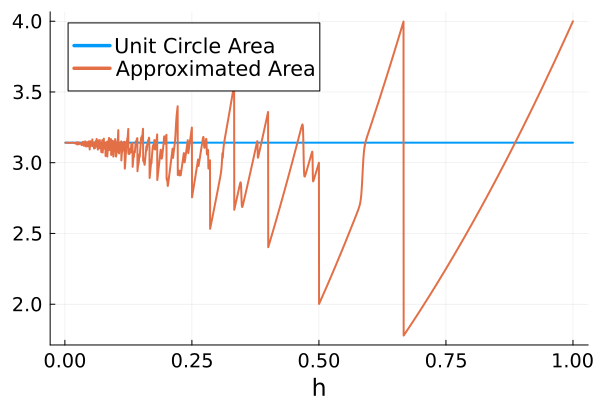
\includegraphics[width=8cm]{quadrature_approximation.png}
		\caption{A plot of $\pi$ (the real area of the unit circle) and the approximated area through the summed up midpoint rule dependent on the mesh step size h.}
		\label{fig:quadr_approx}
	\end{figure}
\end{proposition}

If we take a look at Definition \ref{def:smoothIndicator}, we can see that the smooth indicator function is in $C^2(R)$ if and only if the radius function of the cell is in $C^2(R)$, since all the other functions that occur in this definition are infinitely differentiable. 
Thus, the summed up midpoint rule is numerically convergent if the radius function is twice continuously differentiable over $R$.\\
Figure \ref{fig:quadr_approx} pictures the error of the computation of the area of the unit circle using the summed up midpoint rule dependent on $h$. One can see that the error vanishes as $h \rightarrow 0$.\\
On this foundation we are also able to compute the overlap of two cells. As mentioned earlier, we can simply use the approximation 
\begin{center}
	$A_{C \cap C_{2}} \approx \int_{R_{overlap}} \psi_{C}(\vec{x})\psi_{\zeta}(\vec{x}) d\vec{x}$.
\end{center}
In the implementation of the overlap computation, we operate quite similarly to the computation of the area of a single cell. First, we determine the rectangles $R_{C}$ and $R_{\zeta}$ which overlap their cells. Then, we choose the intersection $R_{overlap} := R_{C} \cap R_{\zeta}$ to be our operating domain. If the intersection of $R_{C}$ and $R_{\zeta}$ is the empty set ,we can finish the computation and say that the overlap is zero, as both cells will neither overlap. \\
Otherwise, we lay a mesh over $R_{overlap}$ and determine the midpoints $\vec{m}_{i,j}$ as in the computation before. From there on, we are ready to apply the summed midpoint rule to approximate the area of the overlap. Correspondent to the approximation from above, we set our function $f$ from Proposition \ref{prop:summedMidpointRule} to be $f = \psi_{C} \psi_{\zeta}$. \\
Figure \ref{fig:contOverlap} demonstrates how the function $\psi_{C} \psi_{\zeta}$ represents the overlap of $C$ and $\zeta$. \\
For now, these are all important functionalities that we need for our CRF model. We are now able to measure a cell's area and whether or how much it interferes with other cells. 
\begin{figure}[]
	\centering
	\begin{subfigure}{0.45\textwidth}
		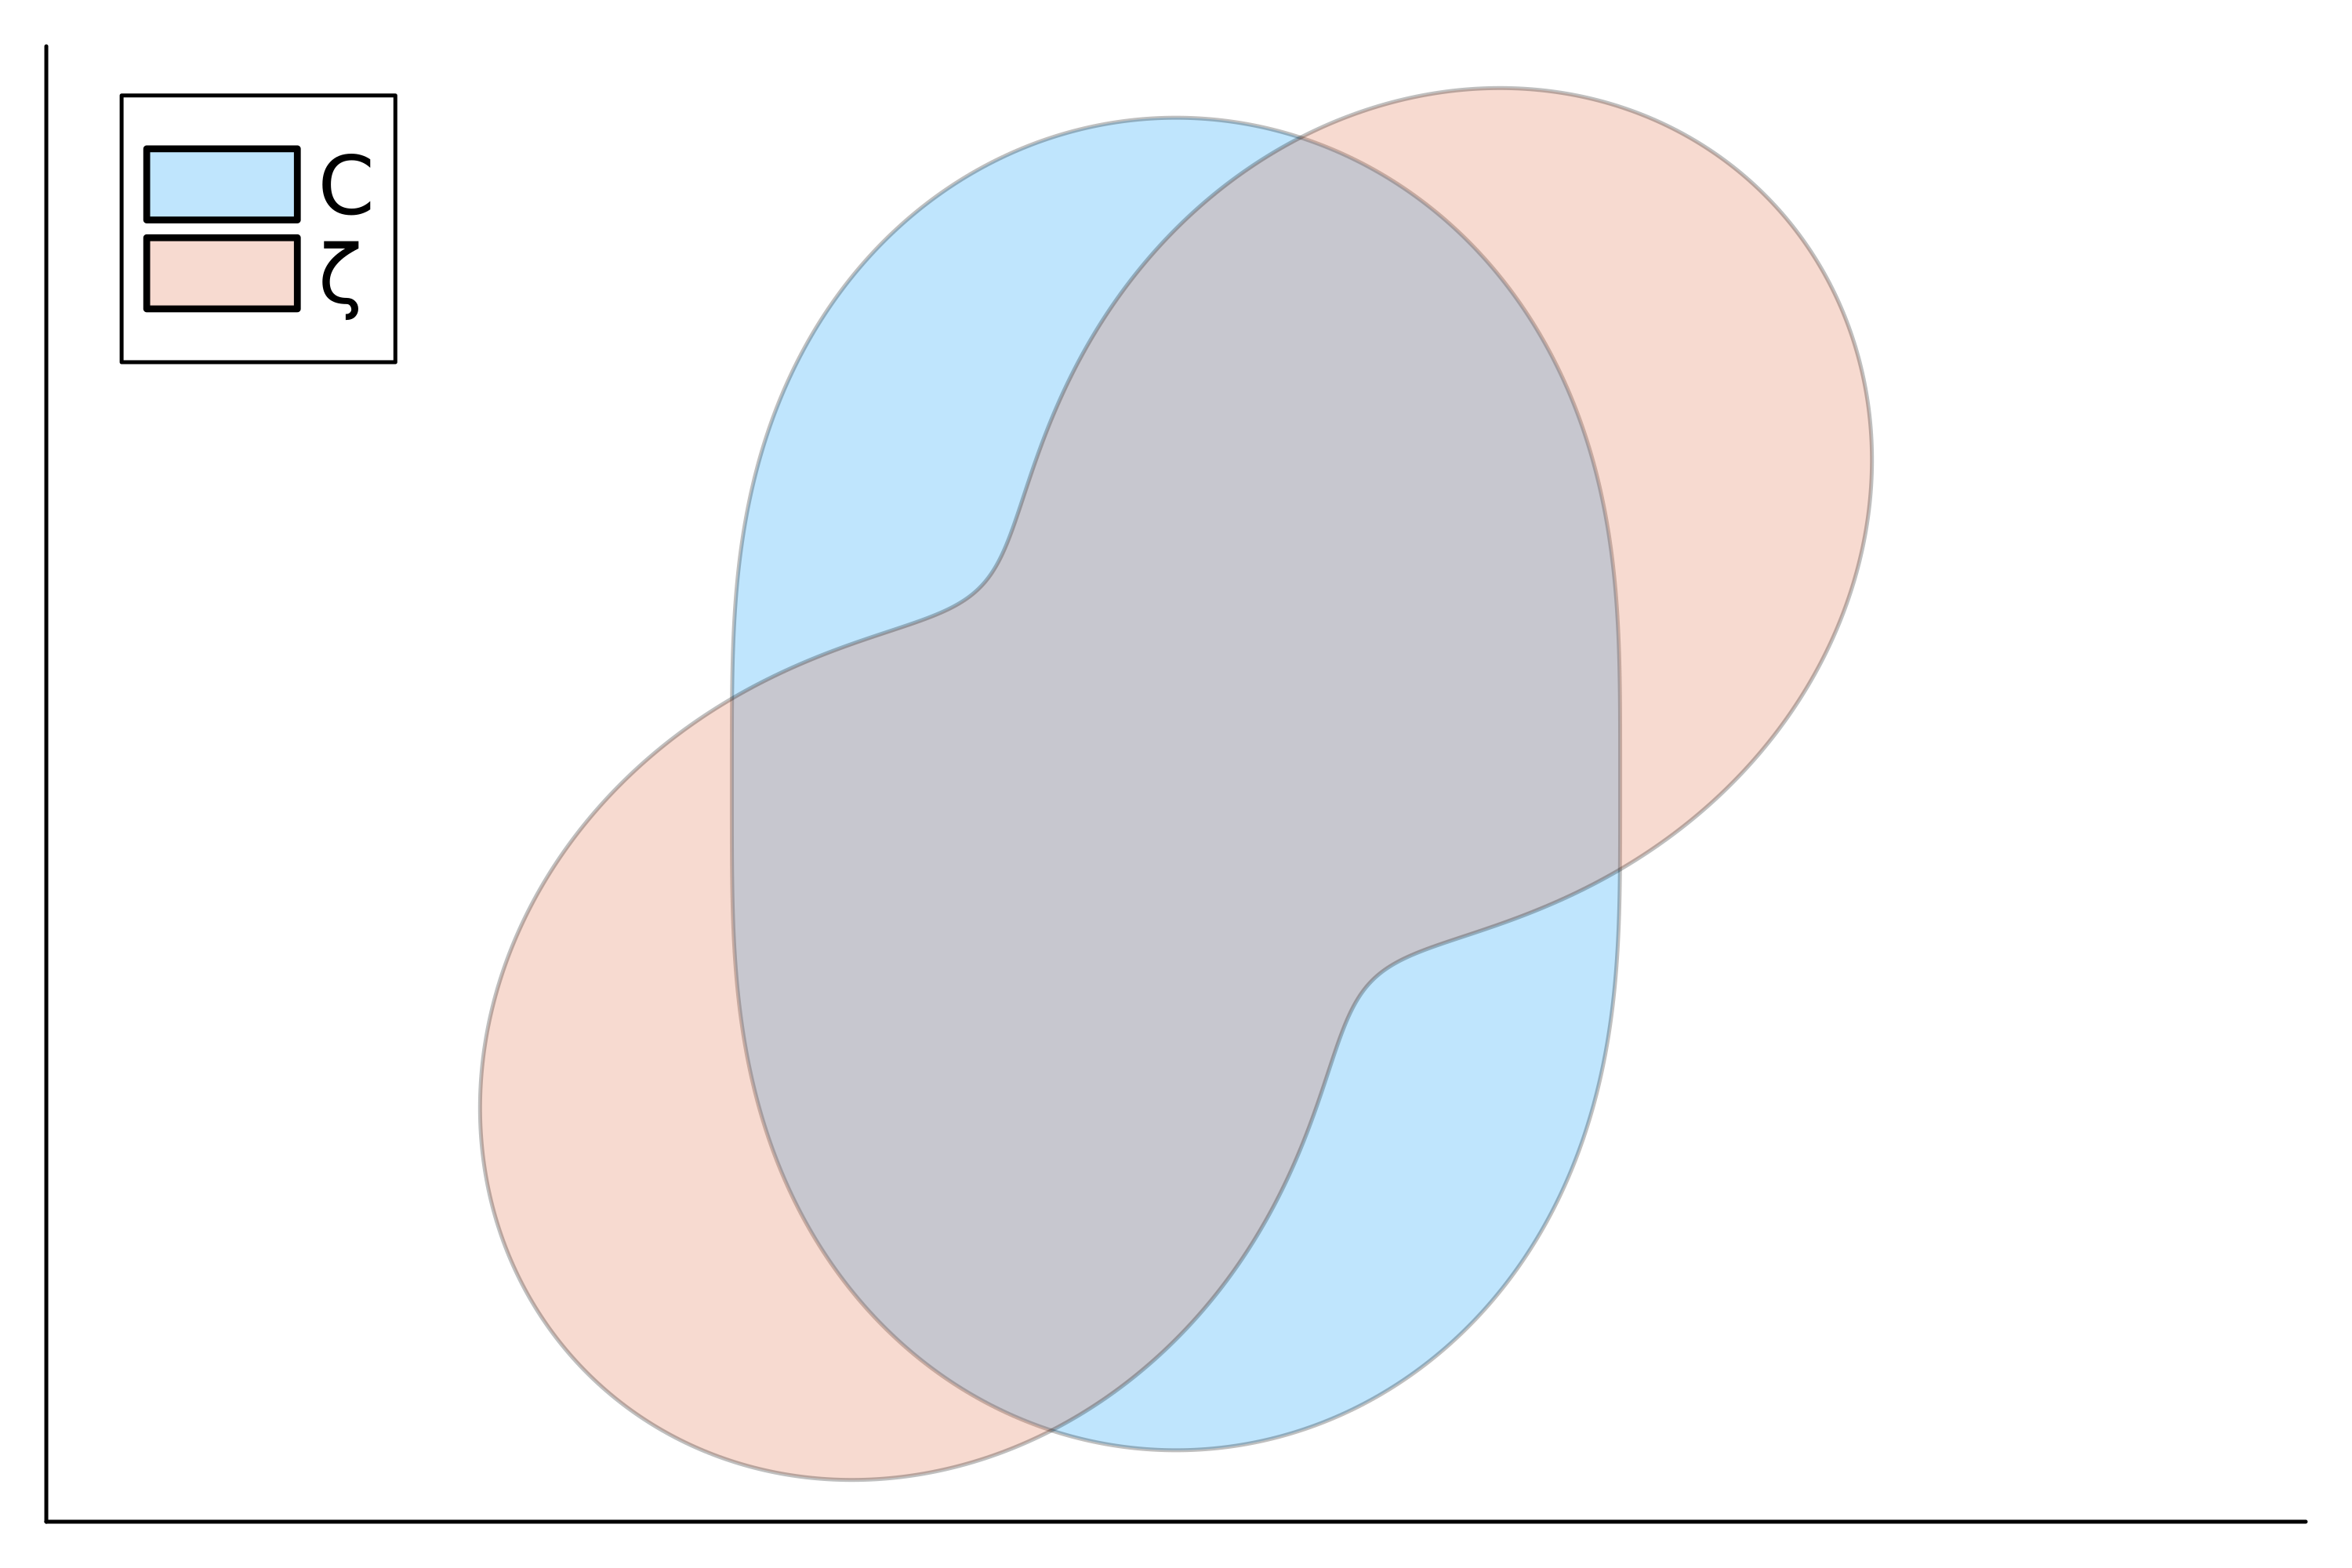
\includegraphics[width=\textwidth]{DisplayContOverlap1.png}
		\caption{First, the figure shows a plot in the plane of $C$ in blue and $\zeta$ in red. The overlap of both cells is clearly noticeable.}
	\end{subfigure}
	\hfill
	\begin{subfigure}{0.45\textwidth}
		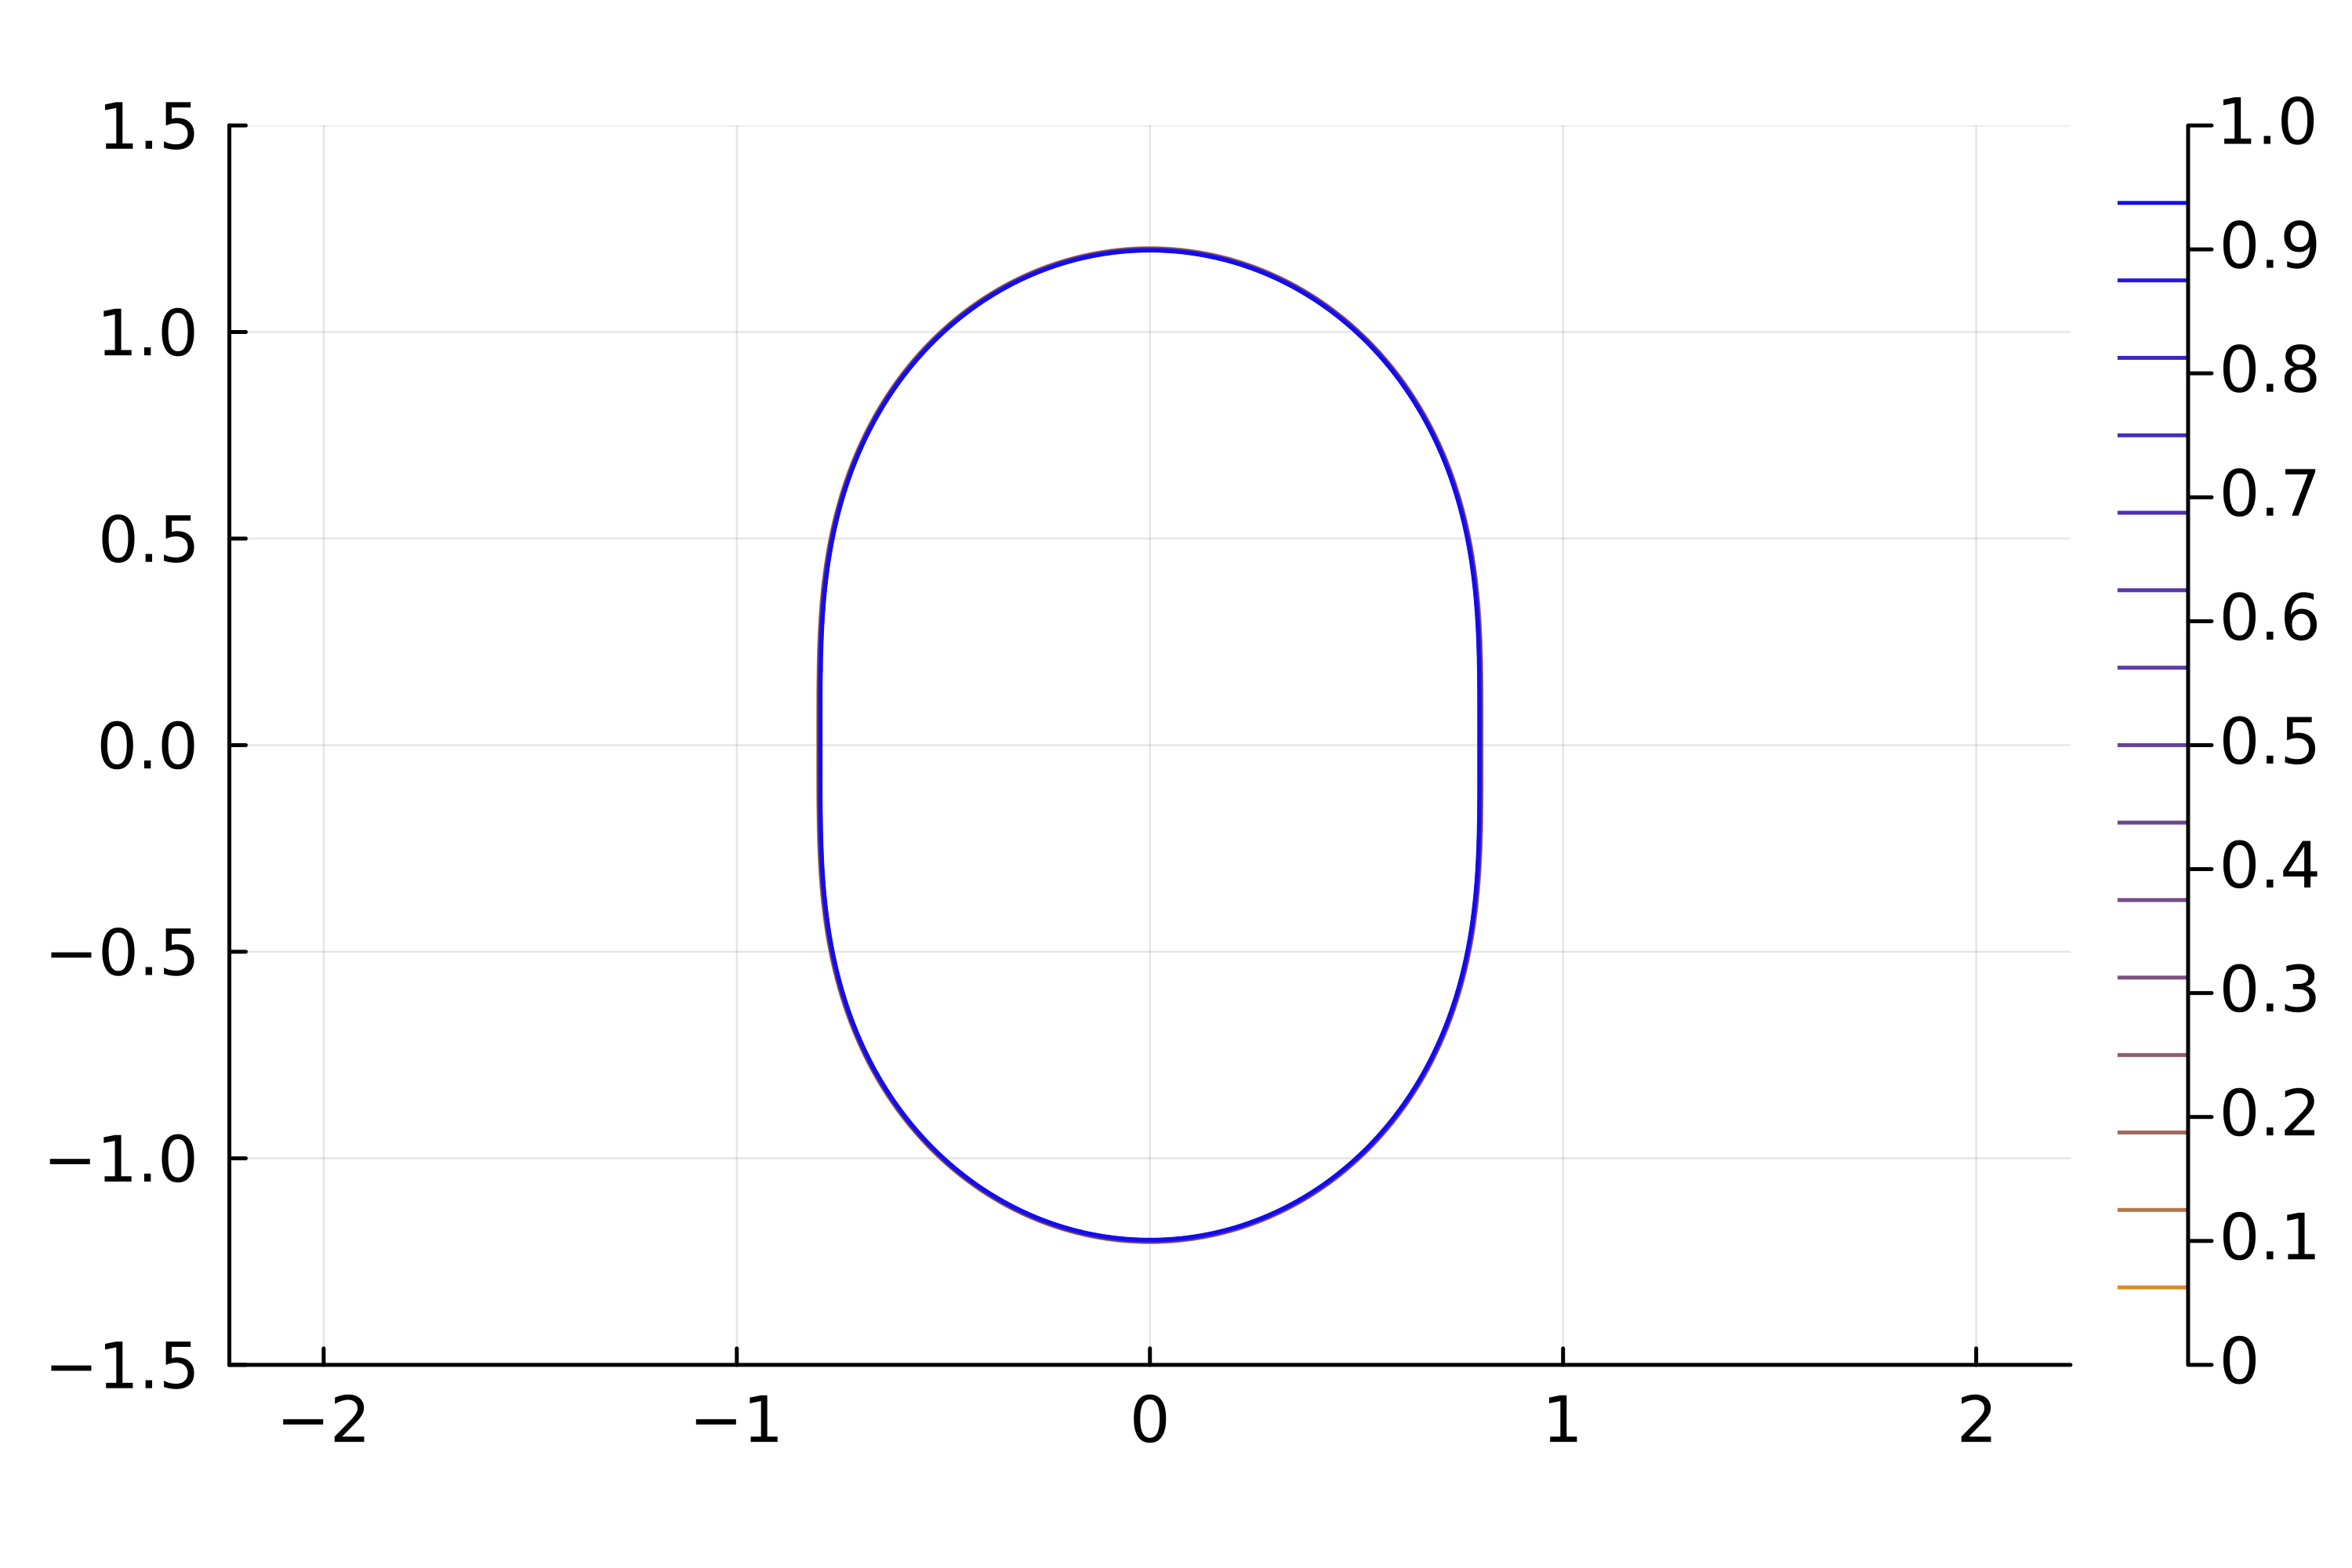
\includegraphics[width=\textwidth]{DisplayContOverlap2_contour.png}
		\caption{The next plot is a contour plot. It displays the function $\psi_{C}$. \\ }
	\end{subfigure}
	\hfill
	\begin{subfigure}{0.45\textwidth}
		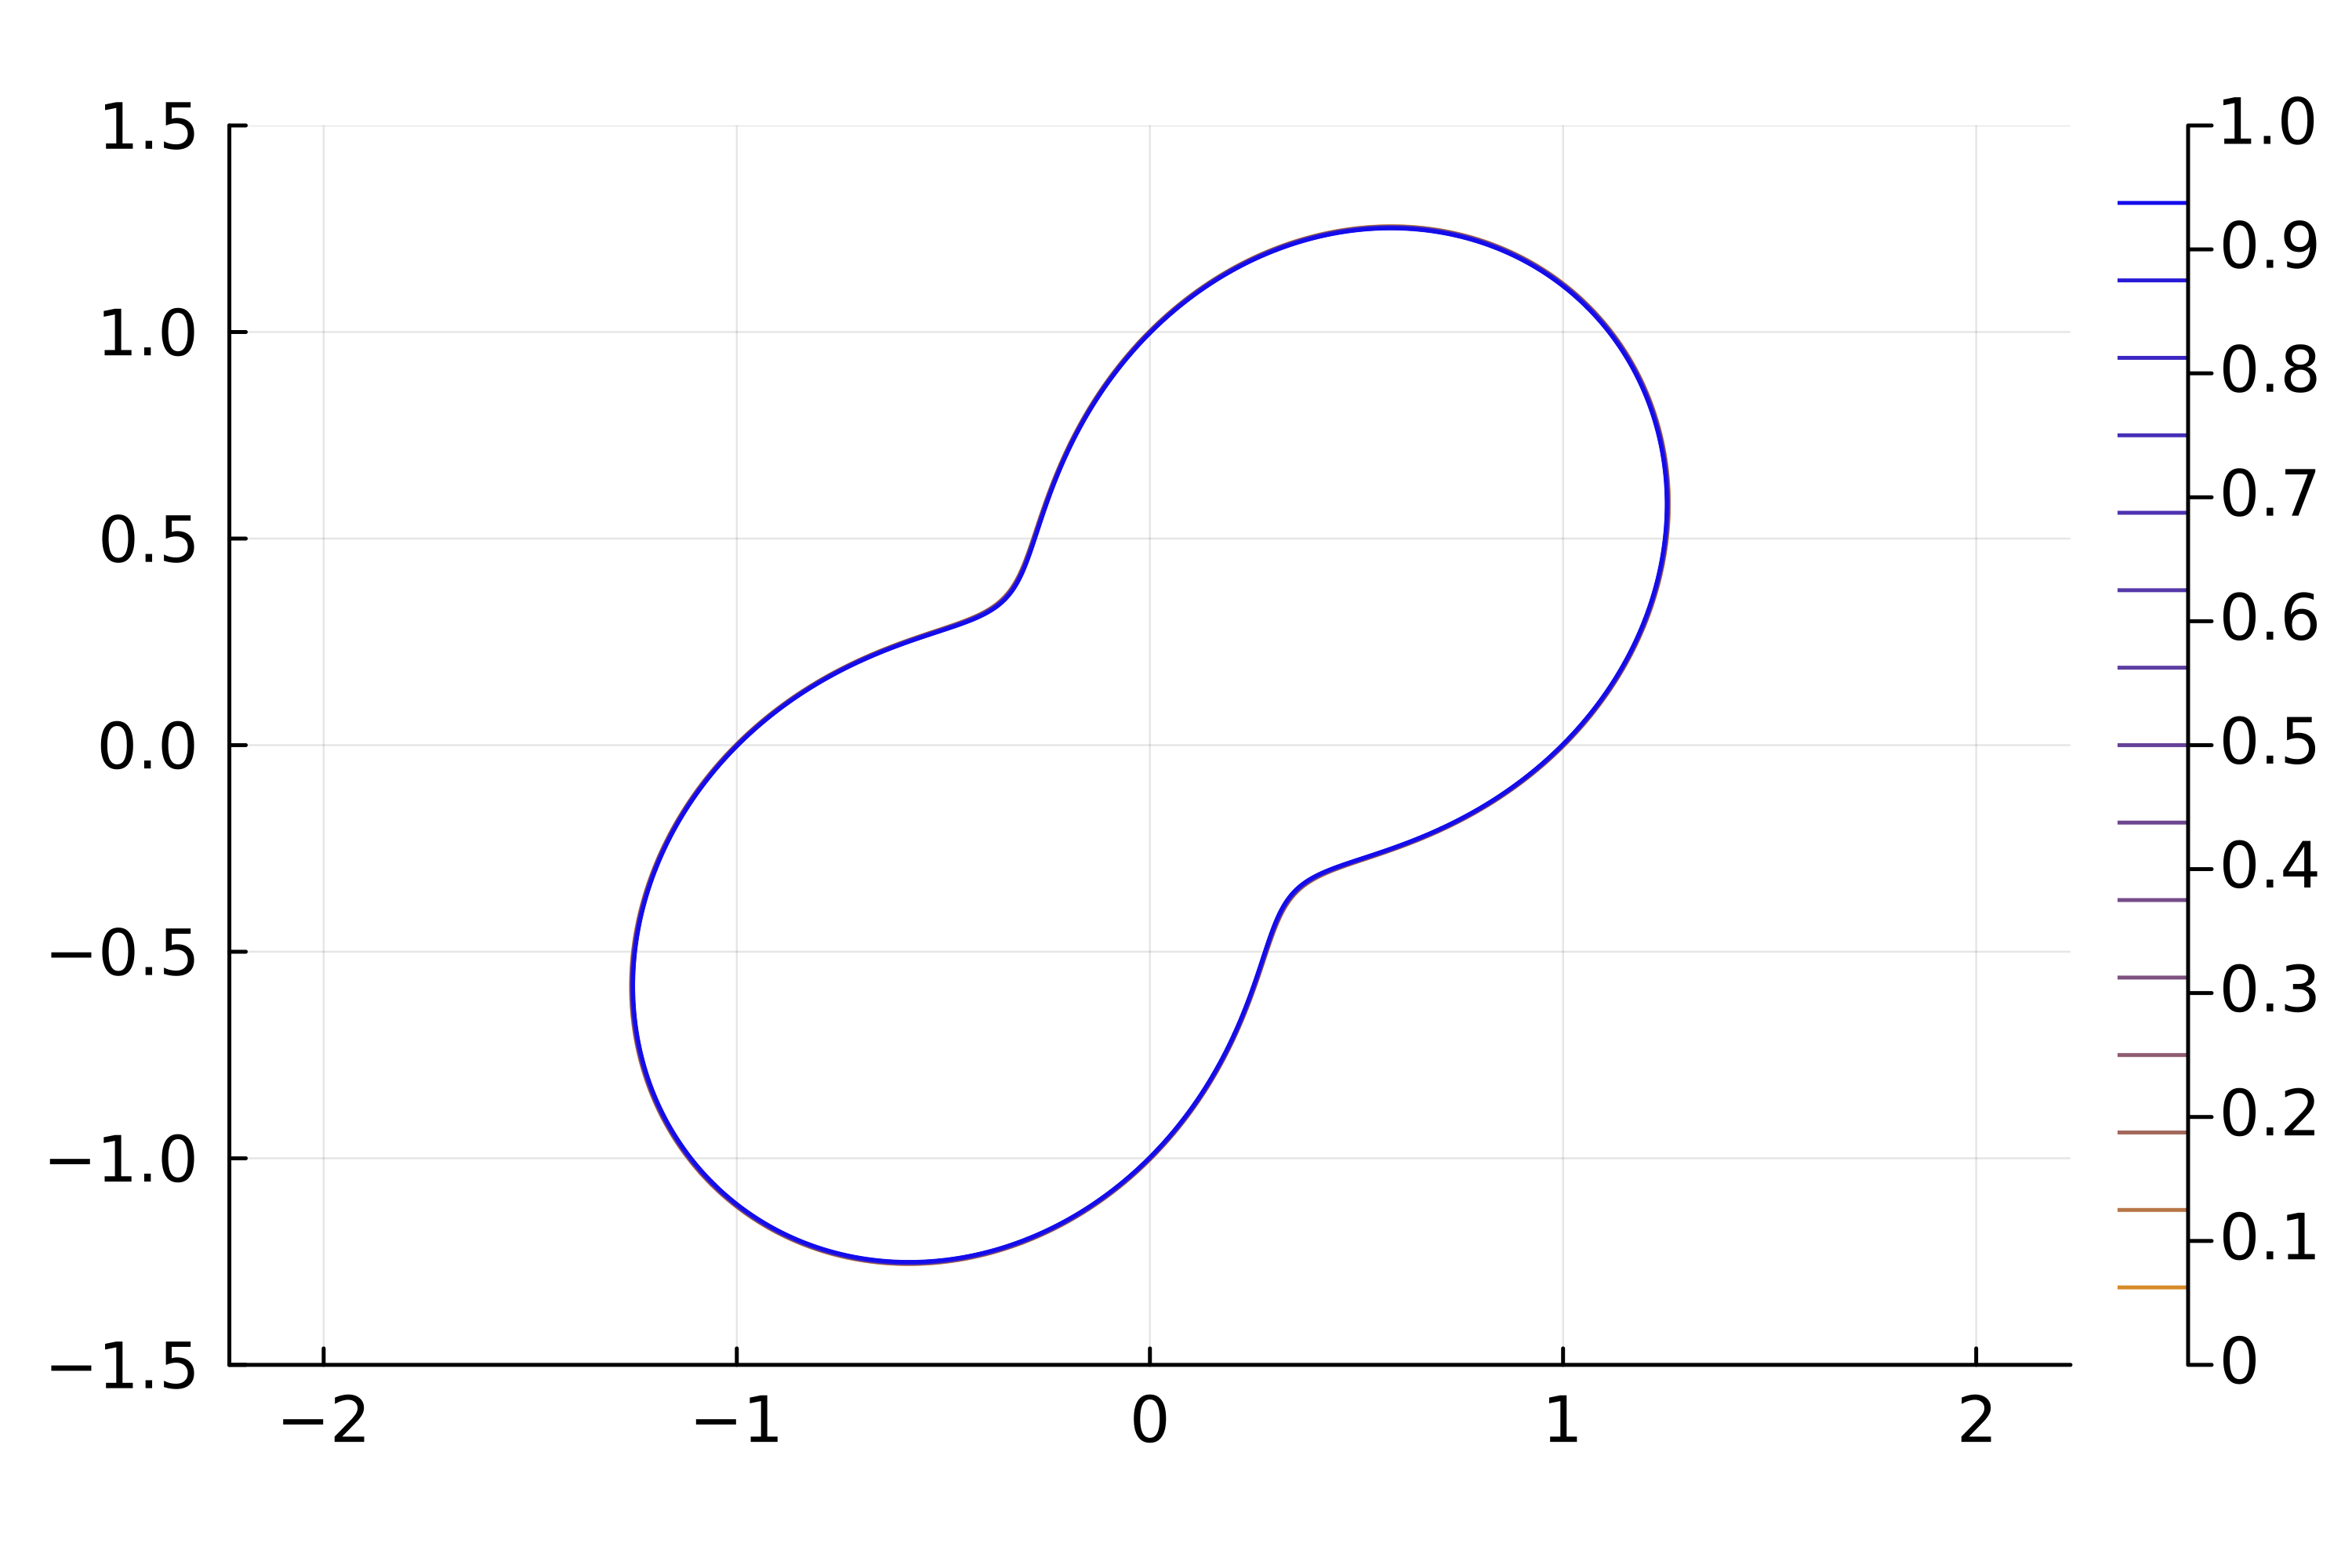
\includegraphics[width=\textwidth]{DisplayContOverlap3_contour.png}
		\caption{In the third sub figure, we can see the counterpart to (b). It shows a contour plot of $\psi_{\zeta}$. }
	\end{subfigure}
	\hfill
	\begin{subfigure}{0.45\textwidth}
		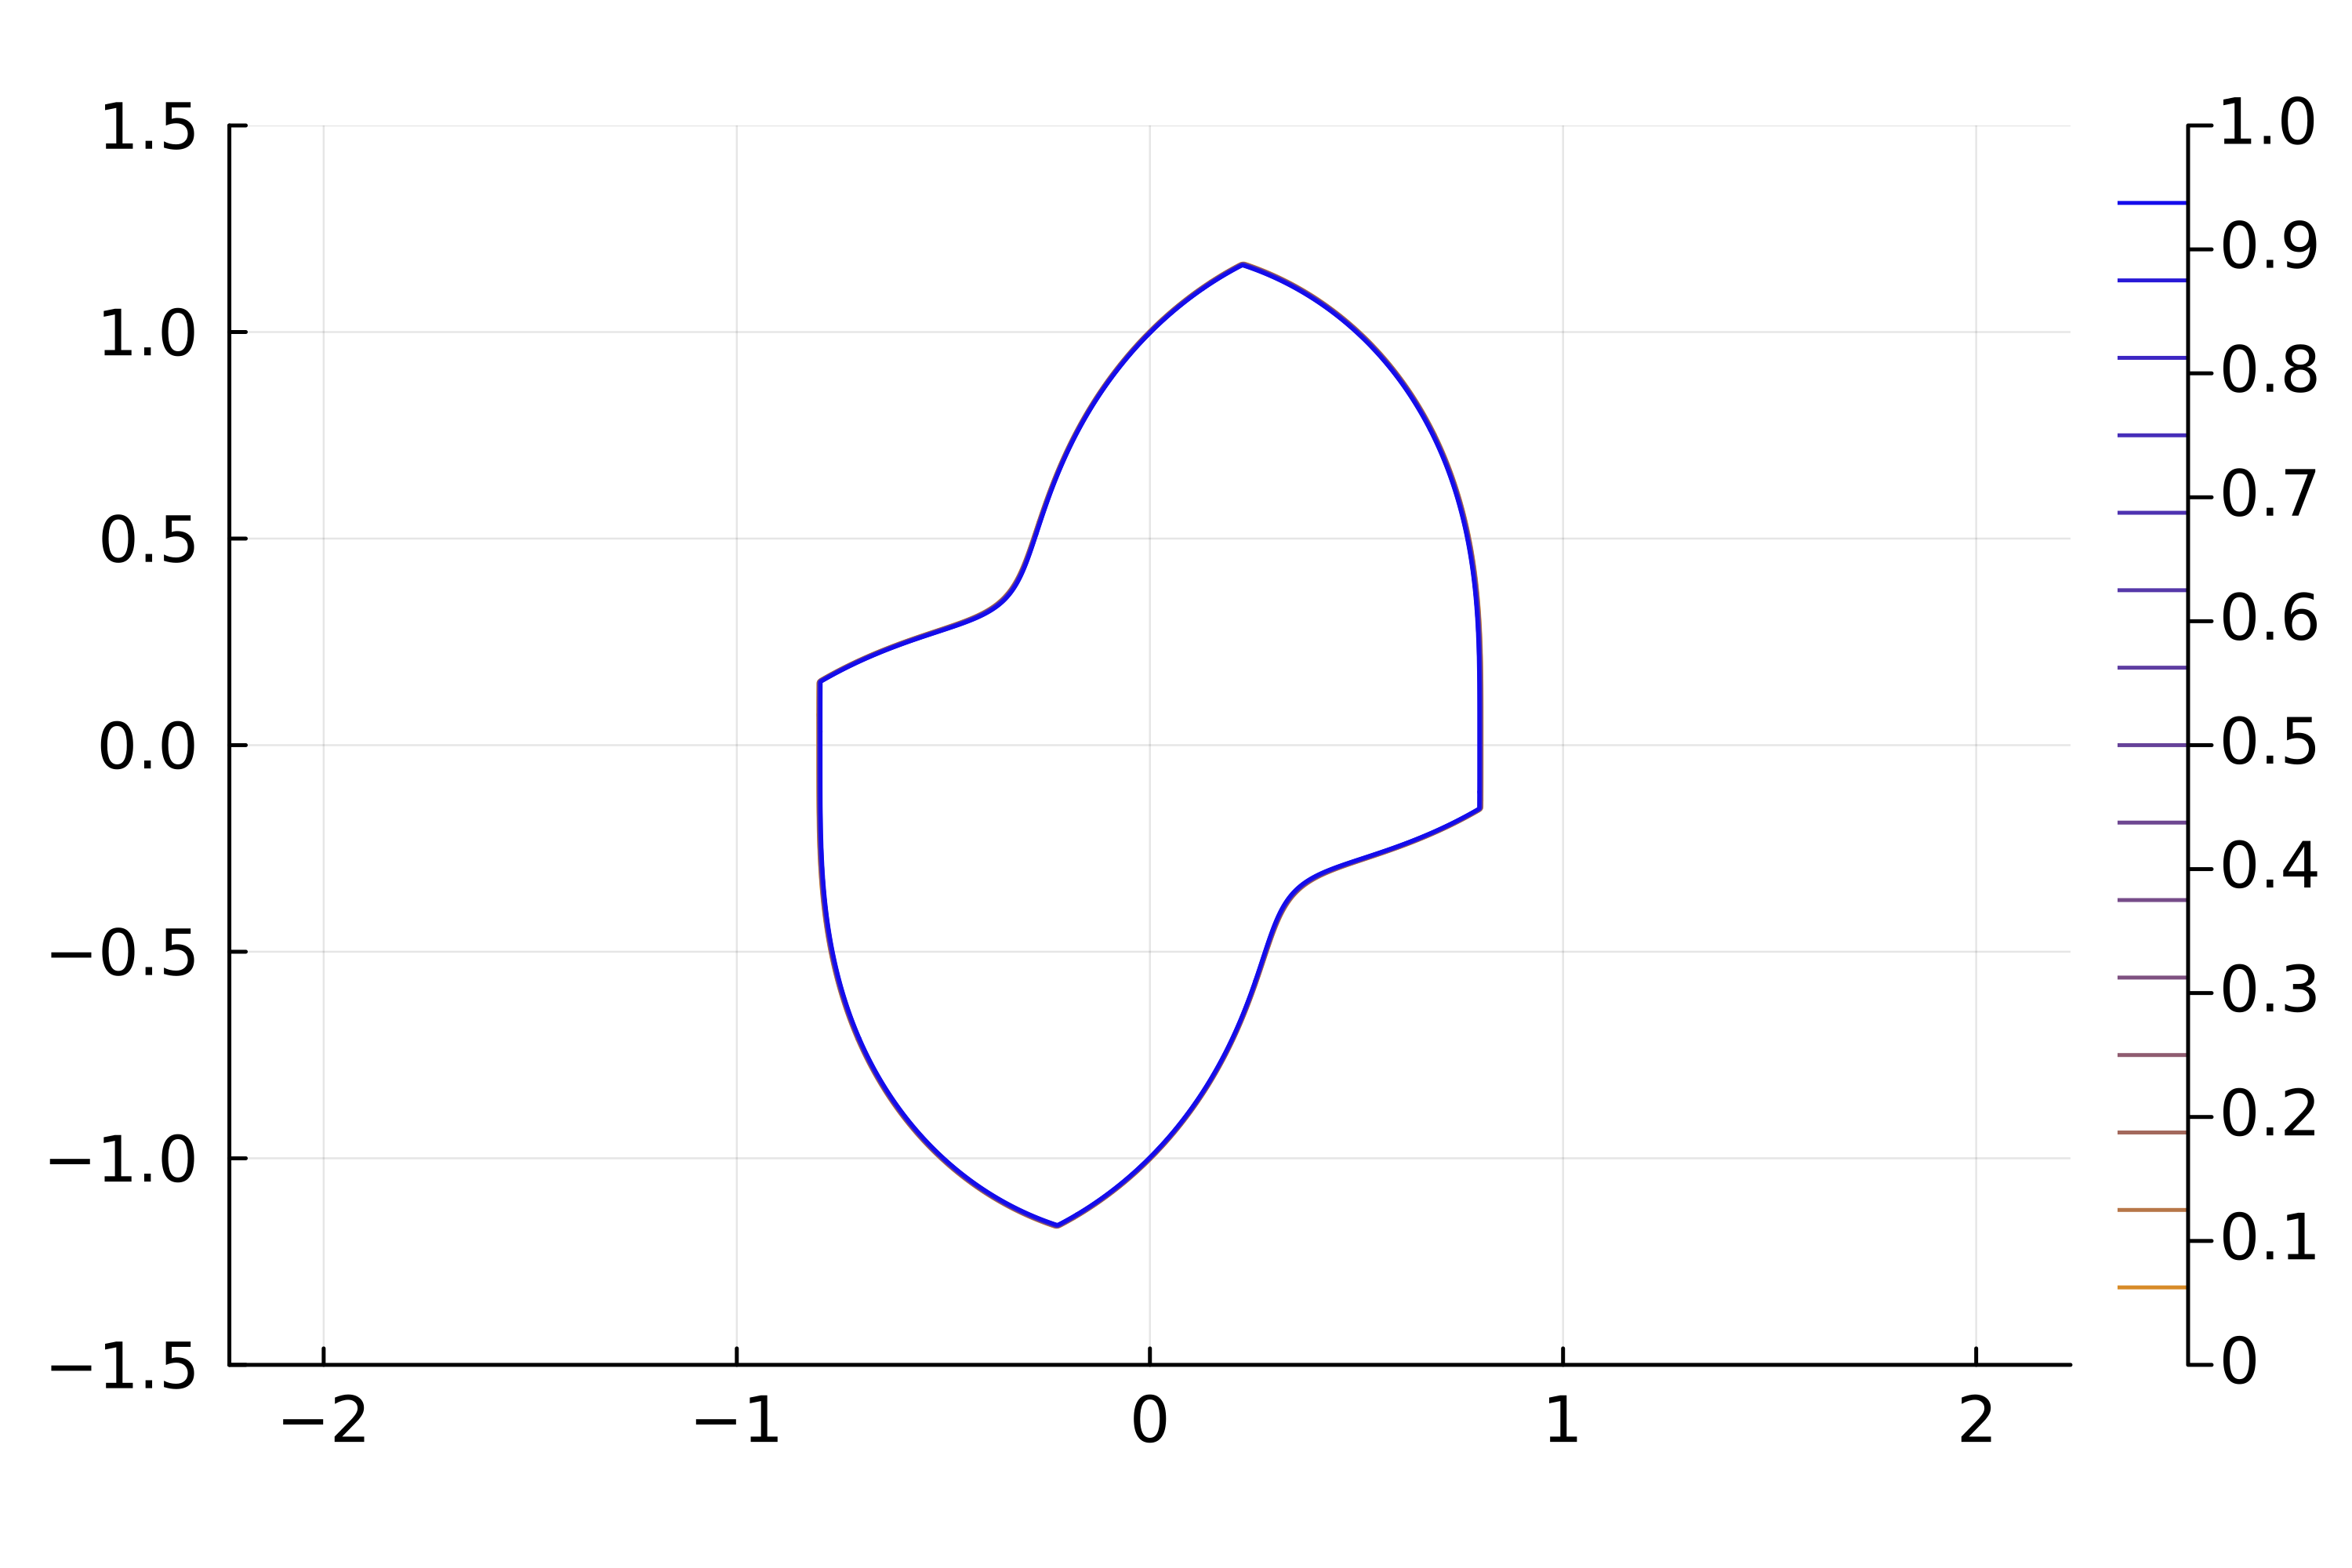
\includegraphics[width=\textwidth]{DisplayContOverlap4_contour.png}
		\caption{A contour plot of $\psi_{C} \psi_{\zeta}$. One can notice the correspondence of this function to the overlap that is visible in (a).}
	\end{subfigure}
	\hfill
	\caption{The graphics show two possible CRF cells $C = ((0, 0)^T, r_{C}(\phi) = \frac{1}{2}\sin(2\phi) + 1)$ and $\zeta = ((0, 0)^T, r_{\zeta}(\phi) = 1 - \frac{1}{5}\cos(2\phi))$, their smooth indicator functions $\psi_{C}$ and $\psi_{\zeta}$ with $s=500$ and demonstrate how the product $\psi_{C}\psi_{\zeta}$ represents the the overlap of the two cells. The axis show the spatial coordinates. }
	\label{fig:contOverlap}
\end{figure}

\subsection{Implementation of the discrete overlap calculation} \label{sec:ImplementationDiscreteOverlap}
The last subsection of Chapter \ref{sec:CellDef} deals with the problem of calculating the overlap of discrete cells. As we have already seen in previous parts, we must therefor determine all overlap areas. They can be represented as discrete cells by themselves. Having obtained all such overlapping cells, it is straightforward to compute their area with the shoelace formula from Proposition \ref{prop:Shoelace}. \\
For the rest of the paragraph, we set the vertex $\vec{x}_{N+1} := \vec{x}_1$. The case in which one cell completely surrounds the other is assumed to be excluded. \\
In spite of the solution displaying to be obvious, the final implementation turns out to be quite effortful. First of all, let us formulate the problem precisely.\\
\begin{problem} \textbf{} \label{problem:overlap}\\ 
	For two cells given in their DF $C = (\vec{c}_1, \ldots, \vec{c}_N)$ and $\zeta = (\vec{\zeta}_1, \ldots, \vec{\zeta}_M)$, identify all discrete cells $O_1, \ldots, O_L$ such that any region where $C$ intersects $\zeta$ is represented by exactly one $O_l$ $, (1 \leq l \leq L)$, i.e.
	\begin{center}
		$
		C_i \cap C_j = \amalg_{l=1}^{L} O_l
		$,
	\end{center}
	where $\amalg$ symbolises a disjointed union and $L$ denotes the number of overlaps that occur between $C_i$ and $C_j$.
\end{problem}
In order to solve this problem, we first define the domain that will be operated on. Similarly to the continuous area computation, we want to approximate the important location through a rectangle in the following way.\\ 
For each of the two discrete cells $C$ and $\zeta$, iterate through all vertices and save those coordinates that are the farthest left, right, up and down. As a result, we obtain two rectangles $R_C \supseteq C$ and $R_\zeta \supseteq \zeta$ which completely cover their corresponding cell. As every overlap is located in both cells and thus in both rectangles, we then set our operation domain as the intersection 
\begin{center}
	$R_{overlap} = R_C \cap R_\zeta$. 
\end{center}
It is simple to control whether $R_C$ and $R_\zeta$ intersect. Therefore, the maximum of the smaller $x$ coordinates of both rectangles must be less than or equal to the minimum of the larger $x$ coordinates of both rectangles. The same must also hold for the $y$ coordinates. The corners of $R_{overlap}$ are then given by these maximum and minimum values. This yields
\begin{center}
	$a = max(R_C^{x_{min}}, R_\zeta^{x_{min}}), \qquad b = min(R_C^{x_{max}}, R_\zeta^{x_{max}})$,\\ \smallskip 
	$c = max(R_C^{y_{min}}, R_\zeta^{y_{min}}), \qquad d = min(R_C^{y_{max}}, R_\zeta^{y_{max}})$,\\ \smallskip
	$a > b \lor c > d \implies R_{overlap} = \emptyset,$ \\ \smallskip
	$a \leq b \land c \leq d \implies  R_{overlap} = [a,b]\times[c,d].$ 
\end{center}
An example of this computation can be seen in Figure \ref{fig:rOverlap}.
\begin{figure}[b!]
	\centering 
	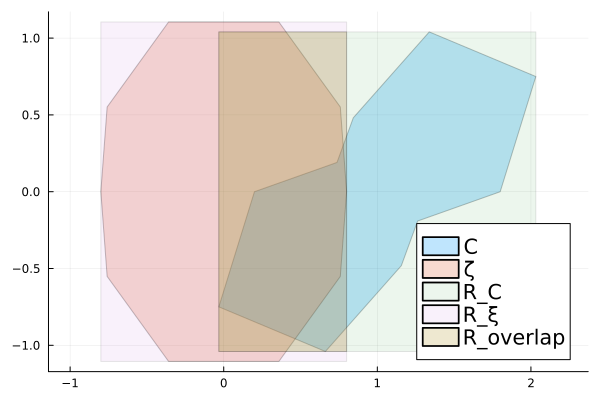
\includegraphics[width=8cm]{discreteOverlap/Roverlap.png}
	\caption{A sample of two discrete cells $C$ (blue) and $\zeta$ (red), their rectangles $R_C$ (green) and $R_\zeta$ (pink) and the intersection $R_{overlap}$ (brown) in the two dimensional space. }
	\label{fig:rOverlap}	
\end{figure}
If performing the intersection delivers an empty set, we can end the calculation, since \textbf{no overlap} is possible in that case. So let us assume that $R_{overlap} \neq \emptyset$ from now on. \\
Now, we want to find every intersection point of the two cells. For the following, it is very useful to introduce some theory about our edges. \\
\begin{definition} \textbf{Edge parameterisation} \label{def:edgeParam}\\
	The edge $e_i$ of the cell $C =  (\vec{x}_1, \ldots, \vec{x}_N)$ is the edge that connects the vertices $\vec{x}_i = (x_i, y_i)$ and $\vec{x}_{i+1}$. \\
	The smallest and biggest $x$ values of $e_i$ are called $x_{i}^{min}$ and $x_{i}^{max}$. Analogously, $y_{i}^{min}$ and $y_{i}^{max}$ represent the lowest and highest $y$ values of $e_i$. They are called boundary coordinates.\\
	An edge $e_i$ is called parameterisable if the path $p_i: [x_{i}^{min}, x_{i}^{max}] \rightarrow \R^2$ that corresponds to $e_i$ can be expressed as
	\begin{center}
		$p_i(x) = \begin{pmatrix}
			x \\ m_i x + a_i 
		\end{pmatrix}$,
	\end{center}
	for some $m_i, a_i \in \R$. \\
	Thus, all edges that are not parameterisable run completely vertically. \\
\end{definition}
Since every edge is just a line, it is no problem to determine $x_{i}^{min}$, $x_{i}^{max}$, $y_{i}^{min}$ and $y_{i}^{max}$. \\
If $e_i$ is a not parameterisable edge, we know that it runs parallel to the $y$ axis. In that case, it is clear that 
\begin{center}
	$x_{i}^{min} = x_{i}^{max} = x_i = x_{i+1} $, \\ \smallskip
	$y_{i}^{min} = \min(y_i, y_{i+1}) $, \\ \smallskip
	$y_{i}^{max} = \max(y_i, y_{i+1})$.
\end{center}
So let us now assume that $e_i$ is a parameterisable edge. This means that there exist real numbers $m_i, a_i \in \R$ such that every $y$ coordinate of each point $\vec{x} = (x,y)^T$ on $e_i$ can be expressed as $y = m_i x + a_i$ for a $x \in [x_{i}^{min}, x_{i}^{max}].$ On this interval the edge is related to an affine linear function. \\
We can directly save $x_{i}^{min}$ and $x_{i}^{max}$ as the minimum and maximum values of $x_i$ and $x_{i+1}$. 
Notice, that an affine linear functions on a compact interval always reaches its maximum and minimum values at the interval ends. 
Since we have got a parameterisable edge, the $y$ values are given by an affine linear function $y = m_i x + a_i$. Thus, the extreme value are given at the interval ends $y_i = m_i x_i + a_i $ and $y_{i+1} = m_i x_{i+1} + a_i$.\\
Consequently, the boundary coordinates of any edge are given by	
\begin{center}
	$x_{i}^{min} = \min(x_i, x_{i+1}) $, \qquad
	$x_{i}^{max} = \max(x_i, x_{i+1}) $, \\ \smallskip
	$y_{i}^{min} = \min(y_i, y_{i+1}) $, \qquad
	$y_{i}^{max} = \max(y_i, y_{i+1}) $. \\
\end{center}
The determination of $m_i$ and $a_i$ of a parameterisable edge is a little bit more difficult, but can still be given through explicit formulas. \\
\begin{proposition}  \textbf{Computation of $m_i$ and $a_i$}\\
	Let $e_i$ be a parameterisable edge. Then, the parameters 
	\begin{center}
		$m_i = \dfrac{y_{i+1} - y_i}{x_{i+1} - x_i}, \qquad a_i = \dfrac{x_{i+1} y_i - x_i y_{i+1}}{x_{i+1} - x_i}$,
	\end{center}
	deliver the edge parameterisation from Definition \ref{def:edgeParam}. \\
	Proof. \\
	The function $f(x) = m_i x + a_i$ is uniquely defined by the equations	
	\begin{itemize}
		\item[(i)]  $f(x_i) = m_i x_i + a_i = y_i$, 
		\item[(ii)] $f(x_{i+1}) = m_i x_{i+1} + a_i = y_{i+1}$. 
	\end{itemize}
	Subtracting (i) from (ii) and rearranging yields
	\begin{center}
		$ m_i = \dfrac{y_{i+1} - y_i}{x_{i+1} - x_i} $. 
	\end{center}
	Substituting this result into (i) and rearranging to $a_i$ provides
	\begin{center}
		$ a_i = y_i - x_i \dfrac{y_{i+1} - y_i}{x_{i+1} - x_i} =\dfrac{x_{i+1} y_i - x_i y_{i+1}}{x_{i+1} - x_i} $.
	\end{center}
	\qed
\end{proposition}
In order to reduce the computational effort, we do not check every edge for an intersection, but only those that could lie in the critical area $R_{overlap}$. We call these edges critical. \\
\begin{definition} \textbf{Critical edge} \label{def:criticalEdge}\\
	An edge $e_i = \overline{ \vec{c_i} \: \vec{c_{i+1}} }$ of a discrete cell $C = (\vec{c}_1, \ldots, \vec{c}_N)$ is said to be critical for a rectangle $R_{overlap}$ if it could intersects with $R_{overlap}$, i.e. 
	\begin{center}
		$[x_{i}^{min}, x_{i}^{max}] \times [y_{i}^{min}, y_{i}^{max}] \cap R_{overlap} \neq \emptyset$.
	\end{center}
	All edges without this characteristic are called not critical. An illustration of critical edges can be found in Figure \ref{fig:criticalEdges}. \\
\end{definition}
\begin{figure}
	\centering
	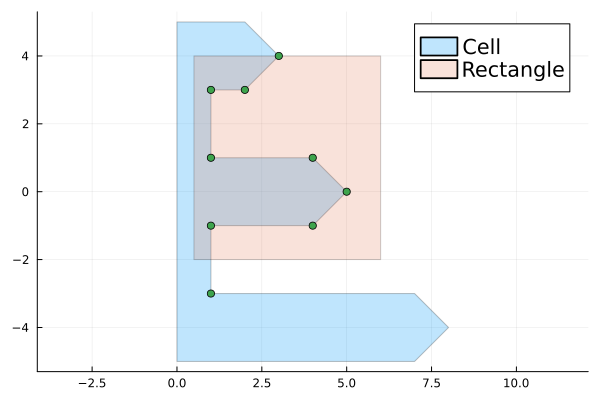
\includegraphics[width=8cm]{discreteOverlap/finding_criticalEdges.png}
	\caption{This diagram shows an example cell (blue), rectangle (red) and the critical edges (green dots) that occur in this scenario. If one traverses vertices counterclockwise, then each dot represents the edge coming afterwards. Every green vertex stands for a critical edge. If a vertex has no dot, the according edge is not critical.}
	\label{fig:criticalEdges}
\end{figure}
Whether the rectangles from the definition intersect or not can be decided in the same way as when calculating $R_{overlap}$. \\
In order to get ahead in the solution of Problem \ref{problem:overlap}, we must calculate all edge parameters of all edges in both DF cells $C$ and $\zeta$. Then, we must determine which edges are critical. Next, we want to find all intersection points of  $C$ and $\zeta$. We save all critical edges and their parameterisations in two sets, one for each cell. \\
For any not critical edge, we can say with certainty that it does not cross or lay inside of $R_{overlap}$ and therefore has no intersection from $C$ and $\zeta$ on it. There could be critical edges that do not intersect $R_{overlap}$ and that thus, do not have an intersection on them as well. However, a further case distinction to decide whether an edge actually intersects with $R_{overlap}$ would be too expensive to serve the purpose of limiting the computational effort. \\
In order to find every intersection from $C$ and $\zeta$, every critical edge in $C$ gets compared with all the critical edges in $\zeta$. The following case distinction always indicates whether two edges intersect or not. The cases should be examined in the exact order now given. Let $e_i$ be a critical edge in $C$ and $\xi_j$ be a critical edge in $\zeta$. \\
\textbf{Case 1: The edges are not nearby.}\\
Similar to the intersection of the rectangles in Definition \ref{def:criticalEdge}, we first want to check whether both edges are close to each other. Therefor, we compute 
\begin{center}
	$R_{intersection} := [x_{i}^{min}, x_{i}^{max}] \times [y_{i}^{min}, y_{i}^{max}] \cap  [x_{j}^{min}, x_{j}^{max}] \times [y_{j}^{min}, y_{j}^{max}] $, 
\end{center}
where the boundary coordinates with a subscript $i$ belong to $e_i$ and the ones with a subscript $j$ belong to $\xi_j$. \\
If this intersection is equal to the empty set, we can end the computation with the result \textbf{no intersection}. Otherwise, we want to save $R_{intersection}$. To reduce the notation effort, we rename the rectangle
\begin{center}
	$R_{intersection} = [a, b] \times [c, d] := [x_{i}^{min}, x_{i}^{max}] \times [y_{i}^{min}, y_{i}^{max}] \cap  [x_{j}^{min}, x_{j}^{max}] \times [y_{j}^{min}, y_{j}^{max}] $,
\end{center}
and proceed with the next case. \\
\textbf{Case 2: Both edges are not parameterisable.}\\
If $e_i$ and $\xi_j$ are not parameterisable, the edges will \textbf{intersect} on the whole line $\{x_i\} \times [c, d]$. Thus, for every $y \in [c, d]$ the point $(x_i, y)^T$ will be an \textbf{intersection} of $e_i$ and $\xi_j$. \\
\textbf{Case 3: Exactly one edge is not parameterisable.}\\
When only one edge, let us say $e_i$, is not parameterisable, we must use the parameterisation of the other edge to compute $s = (x_i, m_j x_i + a_j)^T$. If the $y$ coordinate $m_j x_i + a_j \in [c, d]$, we have found the \textbf{intersection} $s$, but if this is not true, there is \textbf{no intersection} between both edges. \\
\textbf{Case 4: Both edges are parameterisable and $m_i = m_j$.} \label{case:4}\\
Whenever $m_i = m_j$, we must check if $a_i = a_j$. If yes, we again have two edges that intersect on the whole interval $[a, b]$, i.e. one could return the \textbf{intersection} $ (x, m_i x + a_i)^T$ for any $x \in [a, b]$. If $a_i \neq a_j$, both edges do \textbf{not intersect}, because they are parallel, but not the same. \\
\textbf{Case 5: Both edges are parameterisable and $m_i \neq m_j$.}\\
Having reached the final case, we examine lines that always intersect at a $t \in \R$. This $t$ is given by the formula
 \begin{center}
 	$m_i t + a_i = m_j t + a_j \iff t = \dfrac{a_j - a_i}{m_i - m_j}$. 
 \end{center}
 In this case, $e_i$ and $\xi_j$ intersect if and only if $t \in [a, b]$. Then, the \textbf{intersection} is given by the point $(t, m_i t + a_i )^T$. \\
 Otherwise, there is \textbf{no intersection} between $e_i$ and $\xi_j$. \\
\smallskip \\
With the help of this case distinction, we are able to iterate through all critical edges in $C$ and $\zeta$ to find all intersections that occur between these cells. We will call the set of all intersections $I$. Having obtained $I$, we are one step further in our computation. \\ 
If one takes a look at Figure \ref{fig:finalDiscreteOverlap} at the end of this chapter, one can see that each intersection changes whether the overlap cell uses edges from $C$ or edges from $\zeta$. This investigation is the key idea of the algorithm that finally computes the overlap cells. It looks as follows. \\
\begin{algorithm} \textbf{Computation of a discrete overlaps} \label{alge:discreteOverlap}
	\begin{itemize} 
		\itemsep0em 
		\item[] \text{INPUT:}
		\item Discrete cells  $C$and $\zeta$
		\item List $I$ of unused intersections of $C$ and $\zeta$ 
	\end{itemize}
	\begin{algorithmic}
		\Function{constructOverlap}{$C$, $\zeta$, $I$}		
			\State usedIntersections = List$\{$Intersection$\}$(I[1]) 
			\State newOverlap = List$\{$Vertices$\}$(I[1]) 
			\State currentIntersection = I[1]
			
			\For{counter = 1 : length(I)} 
			
				\If{counter is even}
					\State newPath, newIntersection = findPath(currentIntersection, $C$, $I$) 
				\Else 
					\State newPath, newIntersection = findPath(currentIntersection, $\zeta$, $I$) 
				\EndIf
				
				\State append!(newOverlap, newPath)
				\If{newIntersection == I[1]} 
					\State \Return newOverlap, usedIntersections
				\Else 
					\State append!(newOverlap, newIntersection)
					\State append!(usedIntersections, newIntersection) 
					\State currentIntersection = newIntersection
				\EndIf
			\EndFor
		\EndFunction
	\end{algorithmic}
	\begin{itemize} 
		\itemsep0em 
		\item[] \text{OUTPUT:}
		\item A single intersection `newOverlap' which occurs between $C$ and $\zeta$ and which uses vertices from  $C$ and $\zeta$ as well as only intersections from $I$
		\item A list `usedIntersections' of all intersection that are used in `newOverlap'
	\end{itemize}	
\end{algorithm}
The algorithm takes the first intersection $I[1]$ in $I$ as the starting vertex of the overlap cell `newOverlap'. $I[1]$ is also added initially to the list `usedIntersections'. \\
Next, the function `getOverlap' uses another function called `findPath' which delivers the path on the discrete cell $\zeta$ from the starting intersection to the next intersection in $I$ that appears when traversing through the edges of $\zeta$. This new intersection will also be returned. The just mentioned path is a list of vertices in $\zeta$ that exactly occur between both intersections. It may be empty if the next intersection is already found on the same edge where the current intersection is located. The new path and the new intersection will then get appended to `newOverlap'. The new intersection will also get added to the list `usedIntersections'. \\
Since each intersection implies changing the cell from which the overlapping cell uses the edges, `findPath' is now applied to the other cell. Again, it will deliver the next intersection as well as a list of the in between laying vertices. The vertex list always gets appended to `newOverlap'. \\
If the new intersection is equal to the first intersection $I[1]$, we have already constructed the final discrete cell `newOverlap'. Then, `newOverlap' and `usedIntersections' can get returned by `constructOverlap'. \\
Otherwise, we can add the new intersection to `newOverlap' and `usedIntersections' and then, we will have to call `findPath' on the other discrete cell once more and repeat the last part of the algorithm, until we find our starting intersection. \\
Once we are able to extract an overlap from $C$ and $\zeta$, we can delete all used intersections from $I$, because every intersection point is part of exactly one overlap. While $I$ is not empty, we can make a new call to the function `constructOverlap' with the adjusted $I$, to obtain another overlap. When $I$ is empty, we have surely found every intersection of $C$ and $\zeta$ and thus, have solved Problem \ref{problem:overlap}. \\
\smallskip \\
Every time `findPath' gets called, it is questionable in which direction the function should traverse through the vertices of the given cell. But it can be tested in the succeeding way. \\
Starting from the current intersection that is passed into the function, go a little bit in one direction on the edge of the passed cell where the intersection is located. For the then obtained point, examine whether it is located in the other cell, too. If the point is located on both cells, we know that the chosen direction is the right one. Otherwise, we know that we must use the other direction. \\ 
A simple way to investigate whether a point is located in a polygon, is to draw a straight line from the point to the outside of the polygon. Then, the number of intersections of the drawn line and the wall of the discrete cell determines whether the point is inside the polygon or not. The point is located in the inside of the polygon if and only if the number of intersections is odd. \\ 
\smallskip  \\
There are some requirements that $C$ and $\zeta$ must fulfil in order for the Algorithm \ref{alge:discreteOverlap} to work properly. \\
First, the algorithm assumes that each intersection is exactly used one time by exactly one discrete cell overlap. If both cells share a vertex, it can happen that this specific vertex, which will then also be an intersection, is used in two different overlaps. Then, our algorithm will fail, because this intersection point will be deleted after the calculation of the first overlap and accordingly, will be absent from the calculation of the second overlap that uses it. \\
Second, the algorithm cannot handle the situation where two edges partly run on each other. This case can require different amounts of intersections to deal with it. The necessary distinctions are not considered in the presented algorithm. \\
In order for the Algorithm \ref{alge:discreteOverlap} to still work, we add the following procedure before we apply the algorithm: As long as one of the problem cases described occurs, move the whole discrete cell $C$ slightly up and right. This will change the overlap area just a little bit, but causes the algorithm to work properly. \\
Finally, we have now fully derived a scheme which is able to compute all overlapping areas between two discrete cells. Thus, we have a solution to Problem \ref{problem:overlap}. Figure \ref{fig:finalDiscreteOverlap} shows some scenarios of two DF cells and the overlap that is computed by the described algorithm. \\
The overlap cells determined by the algorithm are used for the overlap force in Chapter \ref{sec:overlapEnergy}. 
There, a gradient for the area of the overlap cell gets computed. In order for this calculation not to produce an incorrect sign in the computation of the gradient and also in order to meet the requirement of a positively orientated cell for the shoelace formula, it is necessary that the cell is in a positive orientation, i.e. that the vertices are arranged counterclockwise. As \cite{Bonvallet2009} writes, the orientation of a polygon is positive if 
\begin{center}
	$
	\sum\limits_{n=1}^{N} (x_{n+1}-x_n)(y_{n+1}+y_n) < 0,
	$
\end{center}
where $N$ denotes the number of vertices of the polygon, $\vec{x}_n := (x_n, y_n)^T$ denotes the $n$th vertex of the polygon and $\vec{x}_{N+1} := \vec{x}_1$. After each overlap cell computation, we apply this formula to find out, whether the determined cell has a positive orientation, or not. If the orientation is negative, we reverse the order of the vertices so that the cell ends up positively oriented. \\
This method is designed to deal with all kinds of DF cells, also with all varieties of special cases, that may lead to problems in simpler algorithms. The associated price is that the computational effort is quite high, especially when the number of cell vertices increases. \\
In order to optimize the computational effort, it may be useful to meet further requirements to the discrete cells, like for example convexity. An attempt to do so can be found in the Appendix. \\
\smallskip \\
So far, we have introduced two different models for cells with the CRF and DF model. We have also managed to develop methods to compute the area of a cell as well as the overlap of two cells of the same model. \\
For the rest of the thesis we will focus on giving the cells dynamics. Therefor, we will derive different kinds of differential equations that fulfil different purposes. \\
\begin{figure}[t!]
	\centering
	\begin{subfigure}{0.3\textwidth}
		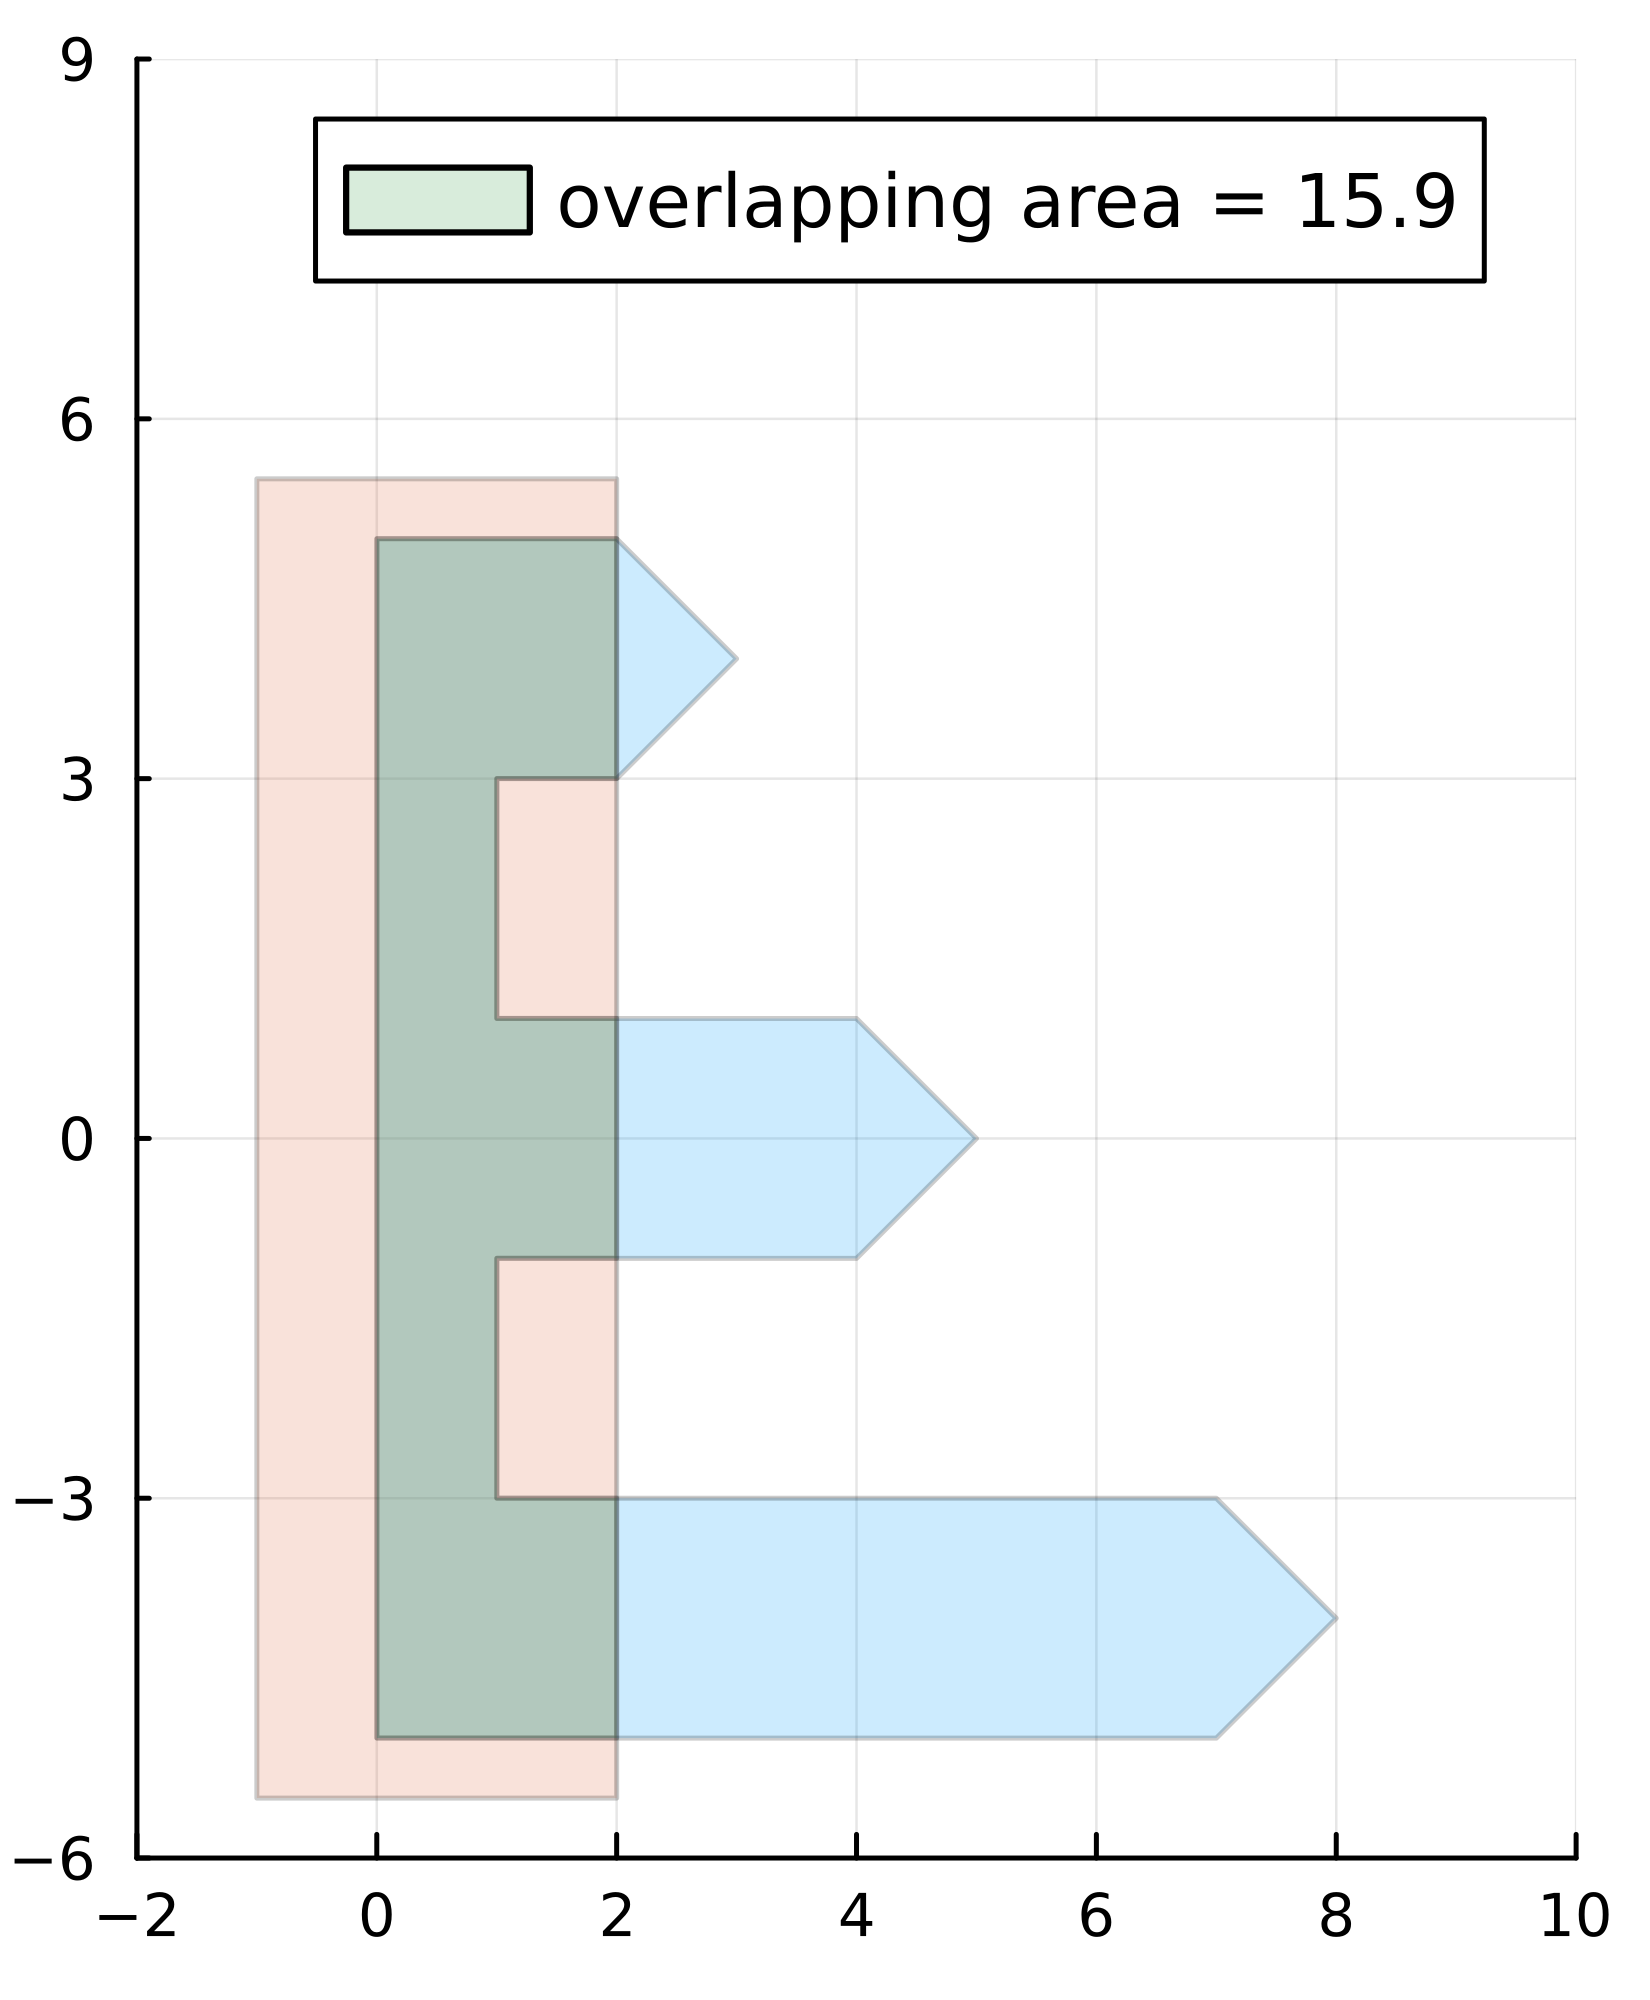
\includegraphics[width=\textwidth]{discreteOverlap/discreteOverlapEx1.png}
	\end{subfigure}
	\hfill
	\begin{subfigure}{0.3\textwidth}
		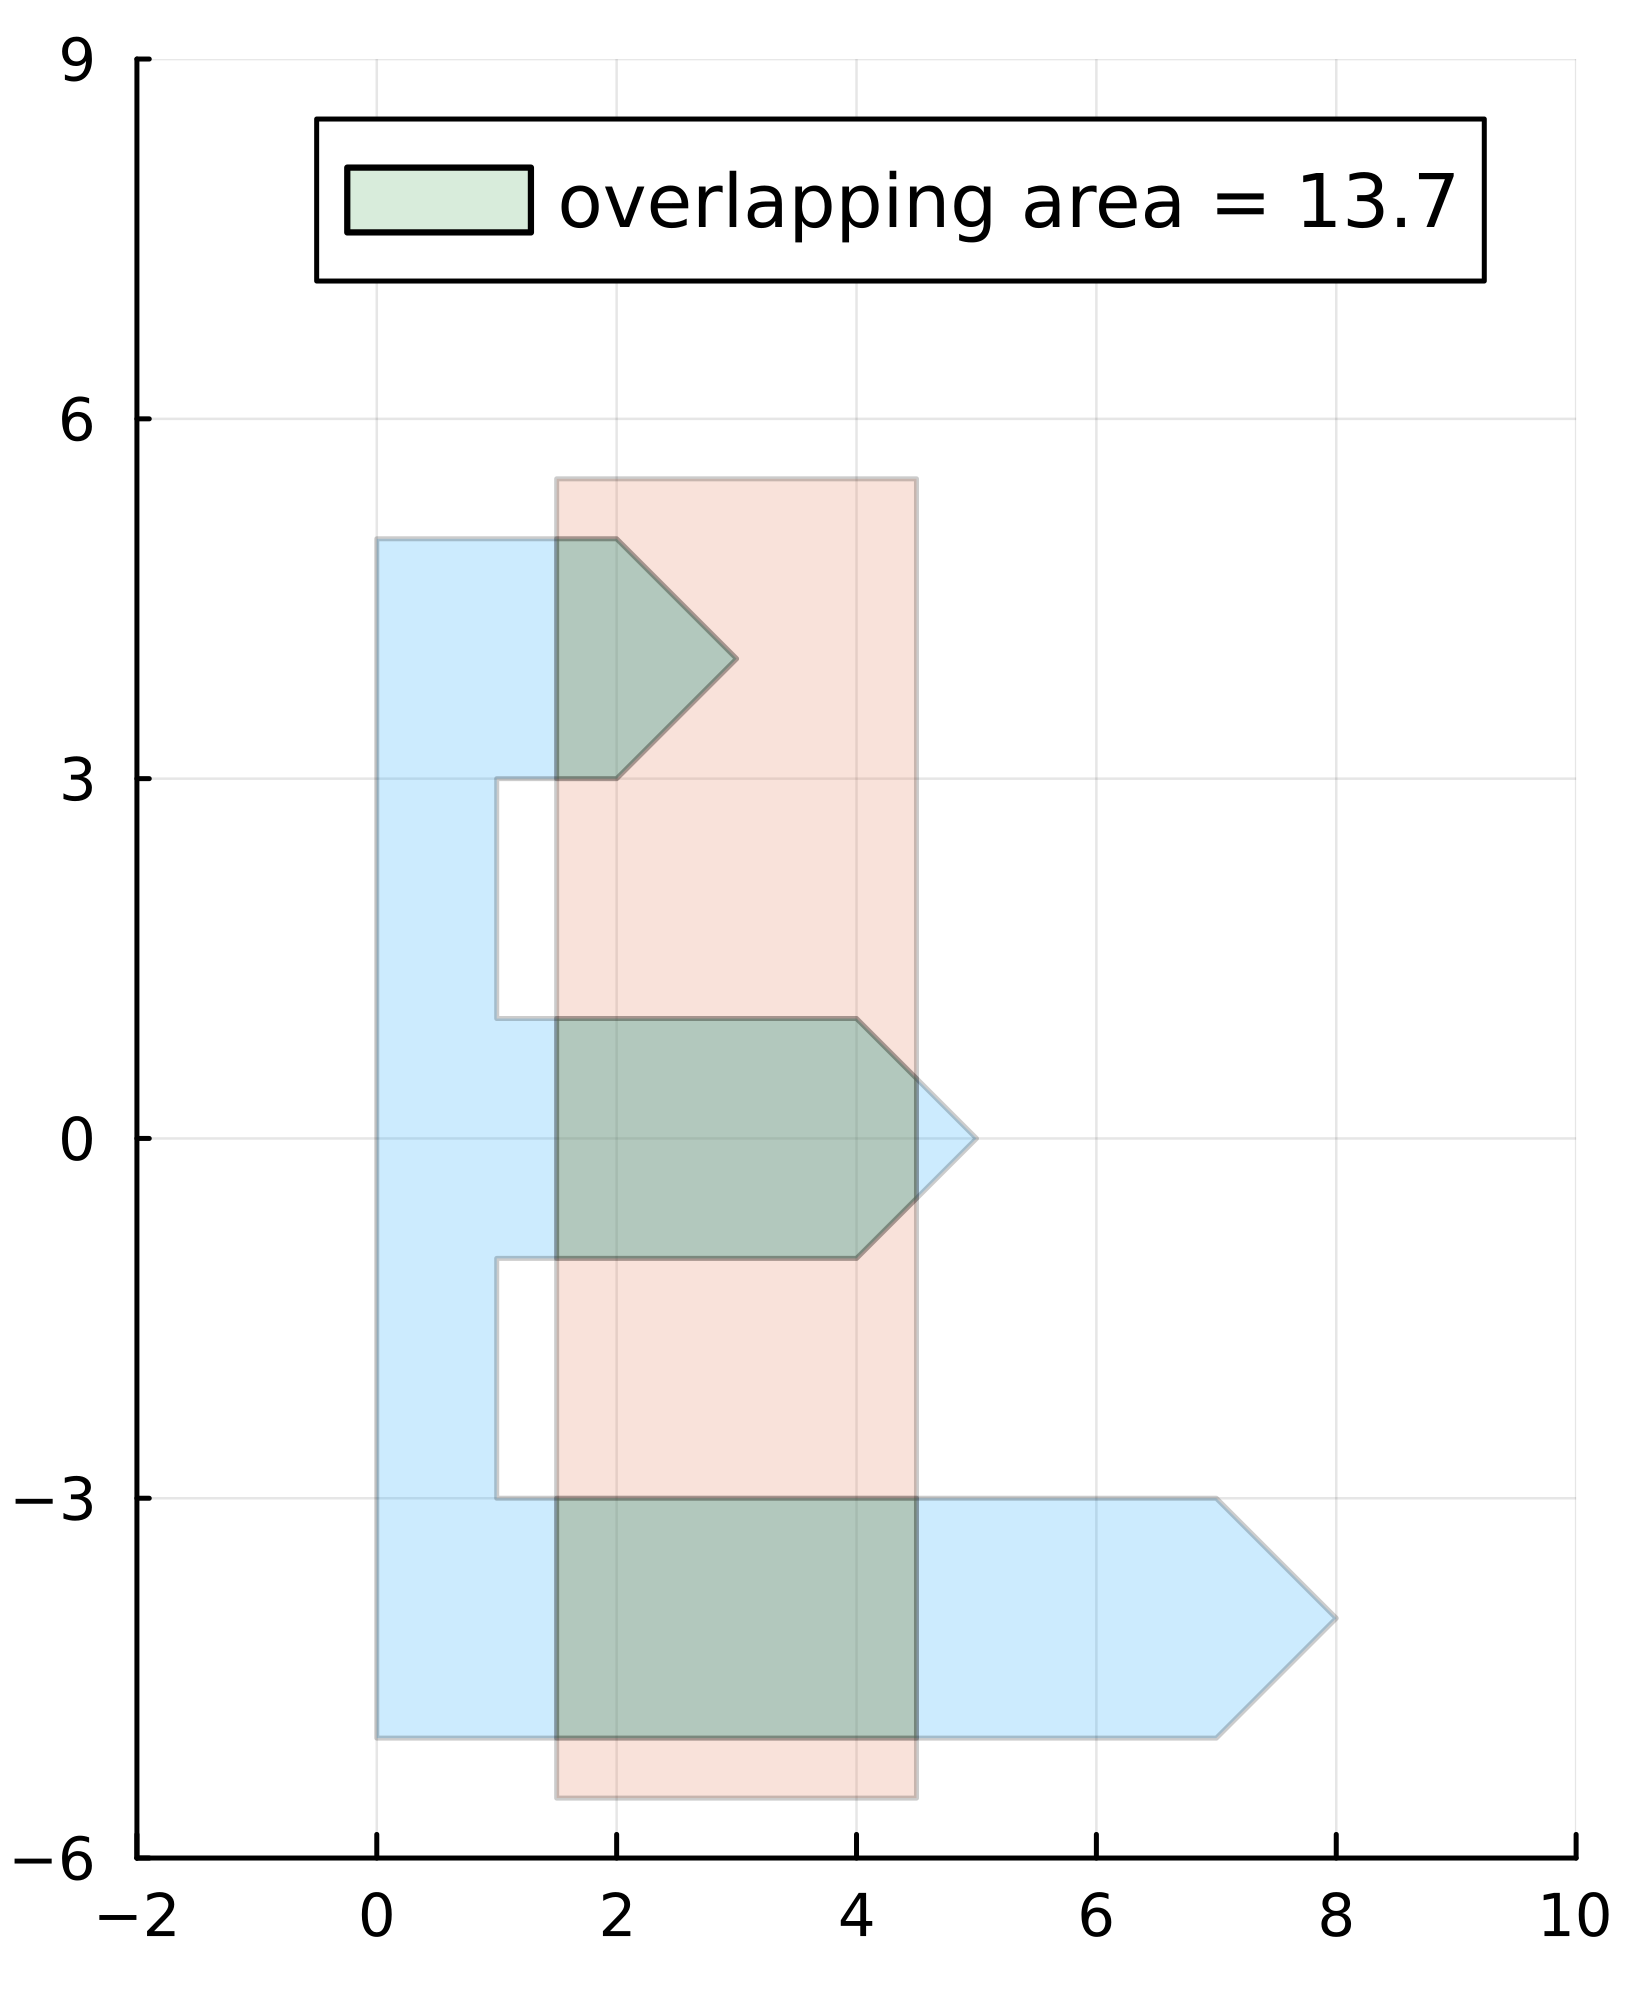
\includegraphics[width=\textwidth]{discreteOverlap/discreteOverlapEx2.png}
	\end{subfigure}
	\hfill
	\begin{subfigure}{0.3\textwidth}
		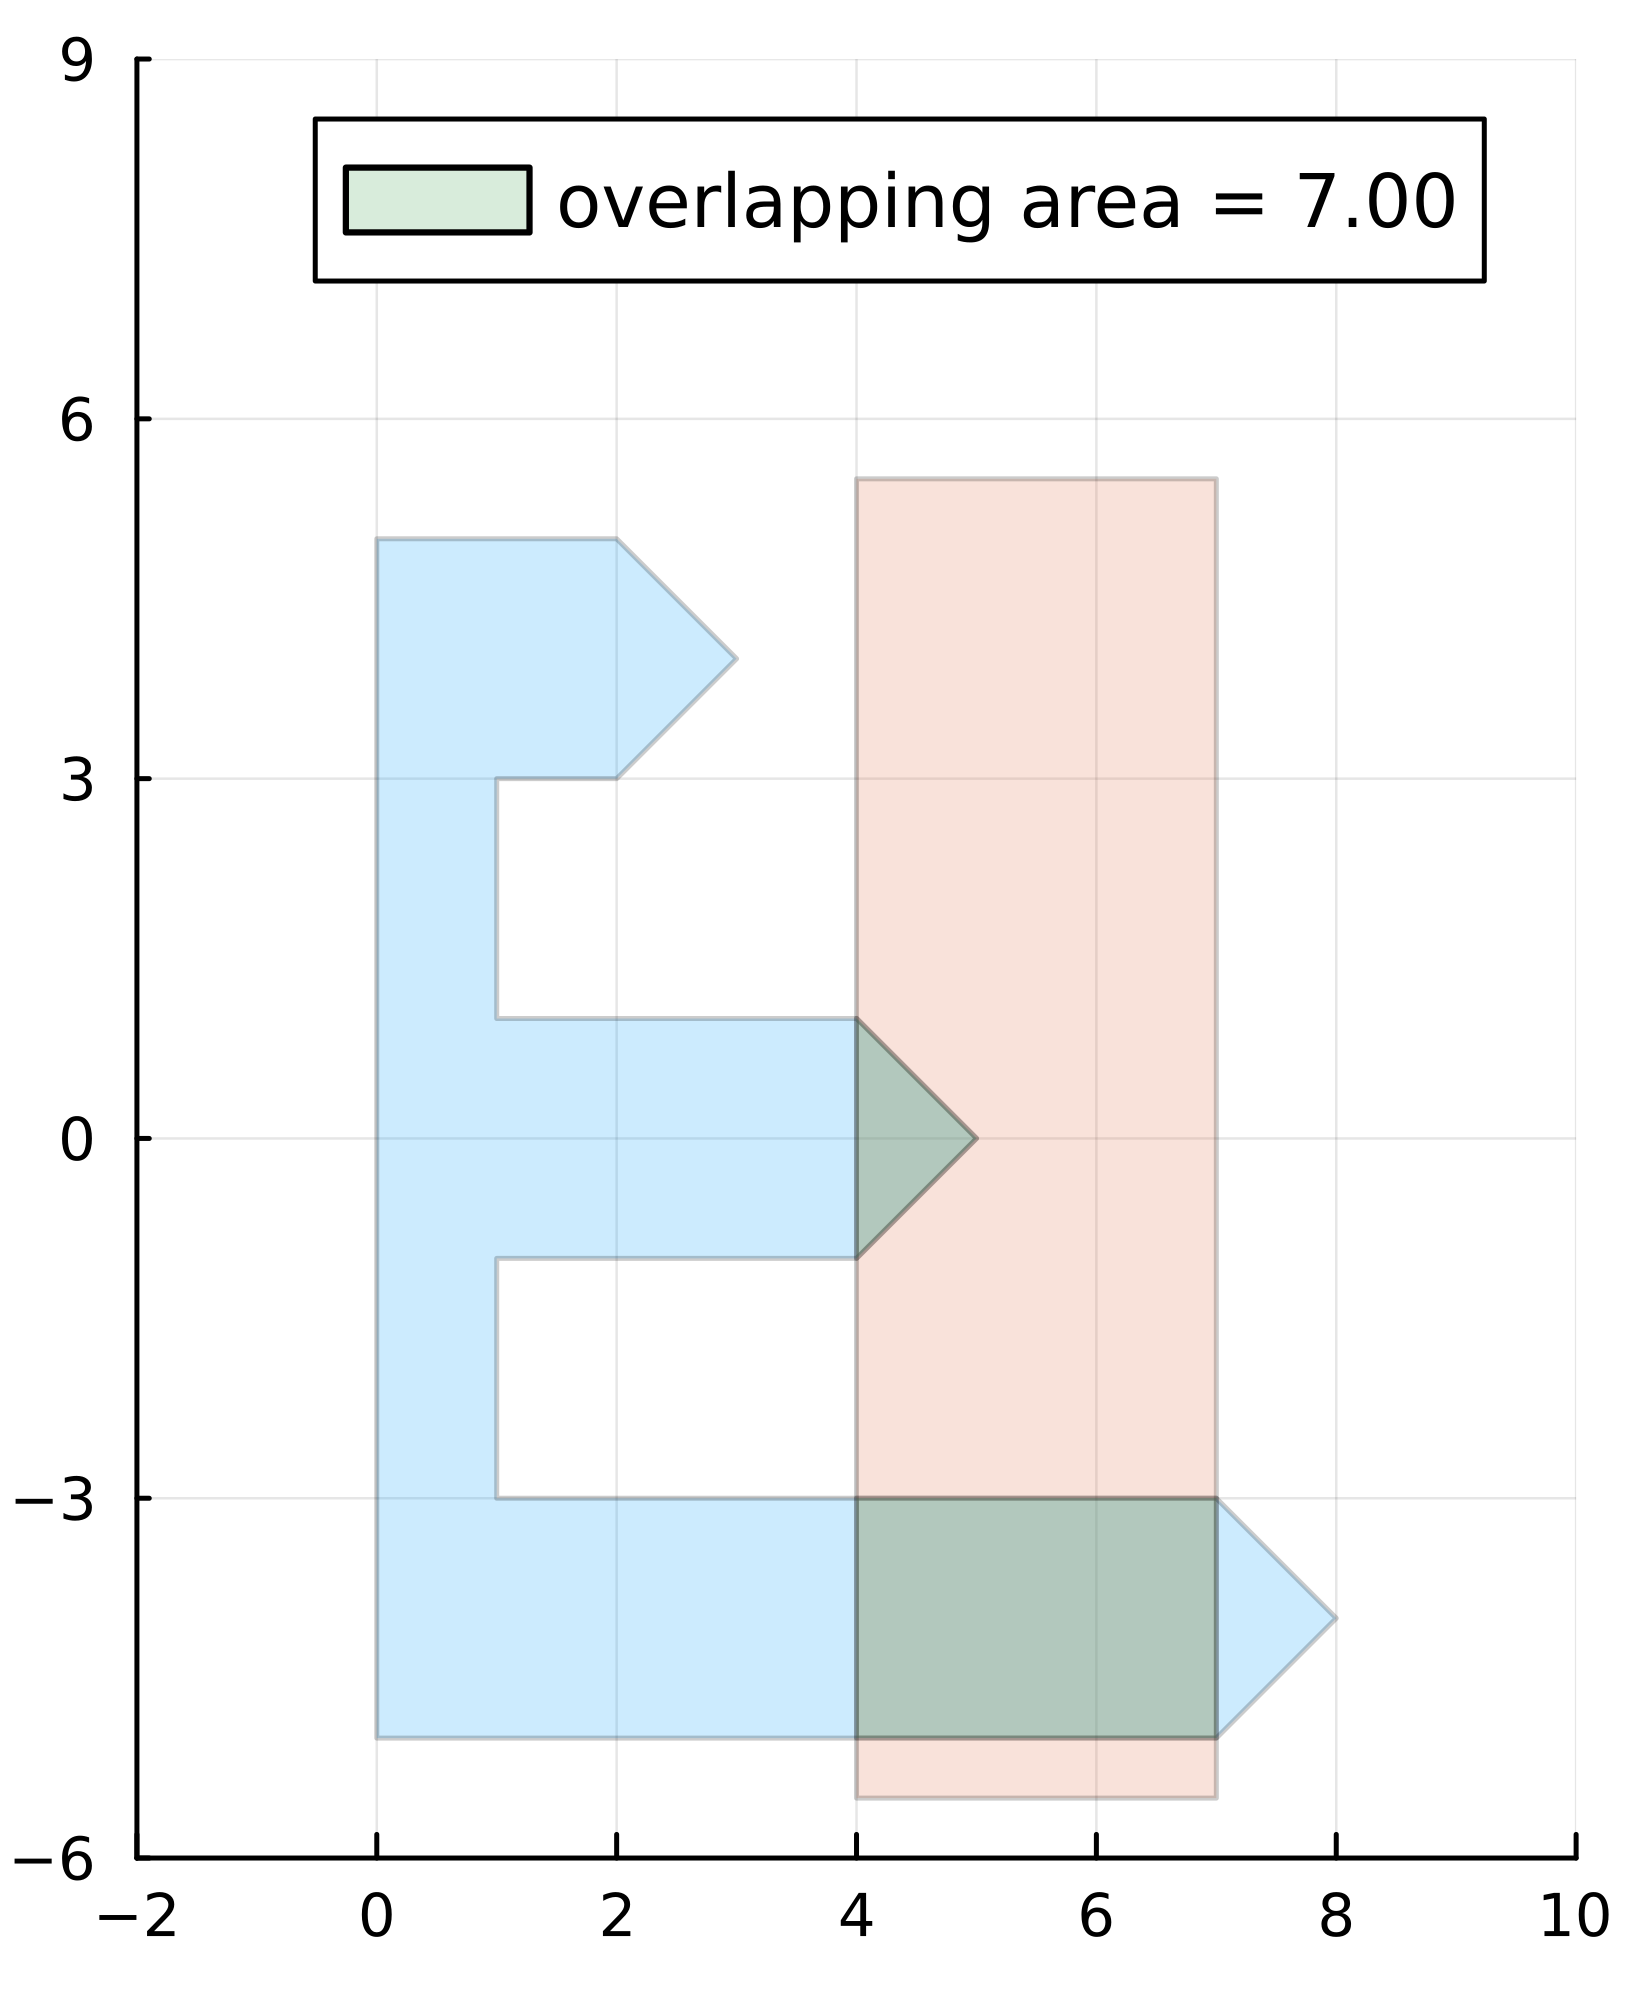
\includegraphics[width=\textwidth]{discreteOverlap/discreteOverlapEx3.png}
	\end{subfigure}\hfill
	\caption{This figure shows 3 plots of 2 DF cells, shown in blue and red, each. One can see the calculated overlap in a green colour and the calculated area of the overlap is shown at the top of the plots. The red cell is shifted to the right in each subsequent plot, resulting in a change of the occurring overlap.}
	\label{fig:finalDiscreteOverlap}
\end{figure}



\newpage
\section{CRF shape recovery model} \label{sec:ShapeRecoveryModel}
Having accomplished the development of the two cell models CRF and DF, we will now start the modelling of some cell dynamics. \\
The very first problem, that we want to regard, looks the following. We are considering one cell $C$ that is given in the CRF $C = (\vec{c}, r)$. In order to give $C$ the possibility to change in time, we make the centre point and radius function dependent on time. Thus, the shape of $C$ at time $t \in [0, \infty)$ is represented by the CRF $C(t) =(\vec{c}(t), r(\phi, t))$. In order to keep the simplicity of ordinary differential equations, every angle $\phi$ gets assigned to its own radius function $r_\phi(t)$ such that for all $t \in [0, \infty)$ and $\phi \in [0, 2\pi)$ the equation $r(\phi, t) = r_\phi(t)$ holds. In order for the analysis to work, we assume $r_\phi \in C^1(\R, \R_{>0})$.\\
There are two specified states in the shape recovery model. The first state is the initial state which is expressed with the CRF $C^{(0)} = (\vec{c}^{\:(0)}, r^{(0)})$. Analogously, the second one is the desired state, described by $C^{(1)} = (\vec{c}^{\:(1)}, r^{(1)})$. To solve our problem, we need to find a model that takes the initial condition $C^{(0)}$ and makes it transform into the desired state $C^{(1)}$, as time goes by. \\
We set
\begin{center}
	$
	 \begin{cases}
	 	
	 	\vec{c}(0) = \vec{c}^{\:(0)}, \\
	 	r_{\phi}(0) = r_{\phi}^{(0)}, & \forall \phi \in  [0, 2\pi),
	 	
	 \end{cases}
	 $
\end{center}
to hold our initial data. \\
After all necessary prerequisites are met, we are ready to introduce the first model provided by three ODEs. \\
\begin{model} \textbf{Shape recovery model}\\
	With the data $C^{(0)} = (\vec{c}^{\:(0)}, r_{\phi}^{(0)})$ and $C^{(1)} = (\vec{c}^{\:(1)}, r_{\phi}^{(1)})$ from above, the shape recovery model is described by the initial value problems (IVPs)
	\[ \left\{
	\begin{array}{ll}
		c_x'(t) = c_x^{(1)} - c_x(t),\\
		c_x(0) = c_x^{(0)},\\
	\end{array}
	\right.
	\]
	\[ \left\{
	\begin{array}{ll}
		c_y'(t) = c_y^{(1)} - c_y(t),\\
		c_y(0) = c_y^{(0)},\\
	\end{array}
	\right.
	\]
	\[ \left\{
	\begin{array}{ll}
		r_\phi'(t) = r_\phi^{(1)} - r_\phi(t),\\
		r_\phi(0) = r_\phi^{(0)},\\
	\end{array}
	\right.
	\]
	where $\vec{c} = (c_x, c_y)^T$. 
\end{model} 
Note, that the preferred states, which are marked with a superscript $(1)$, are just time independent real constants. It is easy to see that all individual IVPs have the same structure
\begin{align} \label{eq:odeContShapeRec}
	\begin{cases}
		x'(t) = a - x(t),\\
		x(0) = b,
	\end{cases}
\end{align}
with $a, b, t \in \R$ and $ x \in C^1(\R, \R)$. This IVP will now be referenced with \eqref{eq:odeContShapeRec}. \\
Hence, the IVPs in the model will have the same analytical characteristics as \eqref{eq:odeContShapeRec}. This is why we will now do the analysis on IVP \eqref{eq:odeContShapeRec}. \\
\begin{proposition} \textbf{Solution of the IVP \eqref{eq:odeContShapeRec}}\\
	The unique global solution of the IVP \eqref{eq:odeContShapeRec} is given by 
	\begin{center}
		$x(t) = (b-a)e^{-t} + a$.
	\end{center}
	Proof. \\
	At the beginning, we want to ensure the existence of a locally unique solution of \eqref{eq:odeContShapeRec} that would be given if the Picard Lindelöf theorem could be applied. Therefor the ODE's rigth hand side $f(t, x) = a - x$ must be continuous in $t$ and Lipschitz continuous in $x$. \\
	As a polynomial of $t$ and $x$, $f$ is in particular continuous in $t$ and $x$. Direct application of the function yields
	\begin{center}
		$|f(t, x_1) - f(t, x_2)| = | a - x_1 - (a - x_2)| = |x_1 - x_2|$, $\forall x_1, x_2, t \in \R$. 
	\end{center}
	Hence, $f$ is Lipschitz continuous in $x$ with constant $L = 1$. \\
	Now, with both conditions met, we can conclude that the Picard Lindelöf theorem can be applied to the IVP associated with the ODE $x'(t) = a - x(t)$ with the initial condition $x(0) = x_0 = b$. This means that there exists a unique local solution in some neighbourhood of $t_0 = 0$. \\
	We now want to determine this solution. Therefor, let us first assume that $a = b$. In that case the right hand side will be zero at $t_0 = 0$ 
	\begin{center}
		$f(t_0, x_0) = a - x(0) = a - b = a - a = 0 $. 
	\end{center}
	Consequently, the initial condition correspond to a steady state and the solution is given by the constant function $x(t) = a = b$. \\ 
	Now, we would like to look at the remaining case $a \neq b$. The right hand side is then initially unequal to zero 
	\begin{center}
		$f(t_0, x_0) = a - b \neq 0$. 
	\end{center}
	Since $f$ is continuous, we can find a small environment $I = [0, \epsilon]$, $0 < \epsilon \ll 1$, of $t_0$ for which we can say that
	\begin{center}
		$\forall t \in I: f(t, x) < 0$ or $ f(t, x) > 0$. 
	\end{center}
	Under these assumptions, the solution can be determined by separating the variables for $t \in I$.
	\begin{itemize}
			\item[] $x'(t) = a - x(t) \iff \int_0^t \dfrac{x'(s)}{a - x(s)} \: ds = \int_0^t 1\: ds = t $
			\item[$\iff$]  $\int_{x_0}^{x(t)} \dfrac{1}{a - v} \: dv = t$ (Substitute $v = x(s)$) 
			\item[$\iff$] $[-\ln(|a - v|) ]_{_{v = x_0}}^{^{x(t)}} = t$
			\item[$\iff$] $ \ln(  \dfrac{a - x_0}{a - x(t)}) = t $ (The condition from before the calculation ensures that the numerator and denominator have the same sign.)
			\item[$\iff$] $\dfrac{a - b}{a - x(t)} = e^t$
			\item[$\iff$] $x(t) = (b - a)e^{-t} + a$ 
	\end{itemize}
	For $a=b$, we regain our first solution $x(t) = a = b$. \\
	All in all, we can conclude that $x(t) = (b - a)e^{-t} + a$ is the locally unique solution of \eqref{eq:odeContShapeRec}. \\
	It is even a global solution, because it fulfils the ODE for any $t \geq 0$. Since $f$ is continuously differentiable on $\R^2$, it is the unique maximal solution. \\
	\qed
\end{proposition}
So the IVP \eqref{eq:odeContShapeRec} has an explicit solution, as does every IVP from the shape recovery model. \\
\begin{corollary} \textbf{Explicit solution to the shape recovery model } \\
	For $C^{(0)} = (\vec{c}^{\:(0)}, r_{\phi}^{(0)})$ and $C^{(1)} = (\vec{c}^{\:(1)}, r_{\phi}^{(1)})$ given, the explicit solution to the shape recovery model is given by the functions
	\begin{center}
		$ c_x(t) = (c_x^{(0)} - c_x^{(1)})e^{-t} + c_x^{(1)} $, \\	\smallskip
		$ c_y(t) = (c_y^{(0)} - c_y^{(1)})e^{-t} + c_y^{(1)} $, \\		\smallskip
		$ r_\phi(t) = (r_\phi^{(0)} - r_\phi^{(1)})e^{-t} + r_\phi^{(1)} $. \\
	\end{center}
\end{corollary}
So, we do not need a numerical implementation to approximate the solution. Figure \ref{fig:shapeRec} shows some shape developments for different initial and desired states. \\
\begin{proposition} \textbf{Steady states of IVP \eqref{eq:odeContShapeRec}} \\
	The only steady state of \eqref{eq:odeContShapeRec} is given by $x^\ast = a$. It is an asymptotically stable steady state. \\
	Proof. \\
	The right hand side $f(x) = a - x$ is equal to zero if and only if $x^\ast = a$. 
	To proof that this state is asymptotically stable, we will use the theorem of linearised stability. Therefor, we must compute
	\begin{center}
		$f'(x) = -1 \implies f'(x^\ast) = -1 < 0$. 
	\end{center}
	Since the value of $x^\ast$ in $f'$ is less than zero, linearised stability yields that  $x^\ast = a$ is an asymptotically stable steady state. \\
	\qed 	
\end{proposition}
It can be deduced from this that in the shape recovery model, the desired state $C^{(1)}$ will always be reached, as $t \rightarrow \infty$, because $a$ is here always associated with the according desired state. 
\begin{figure}
	\centering
	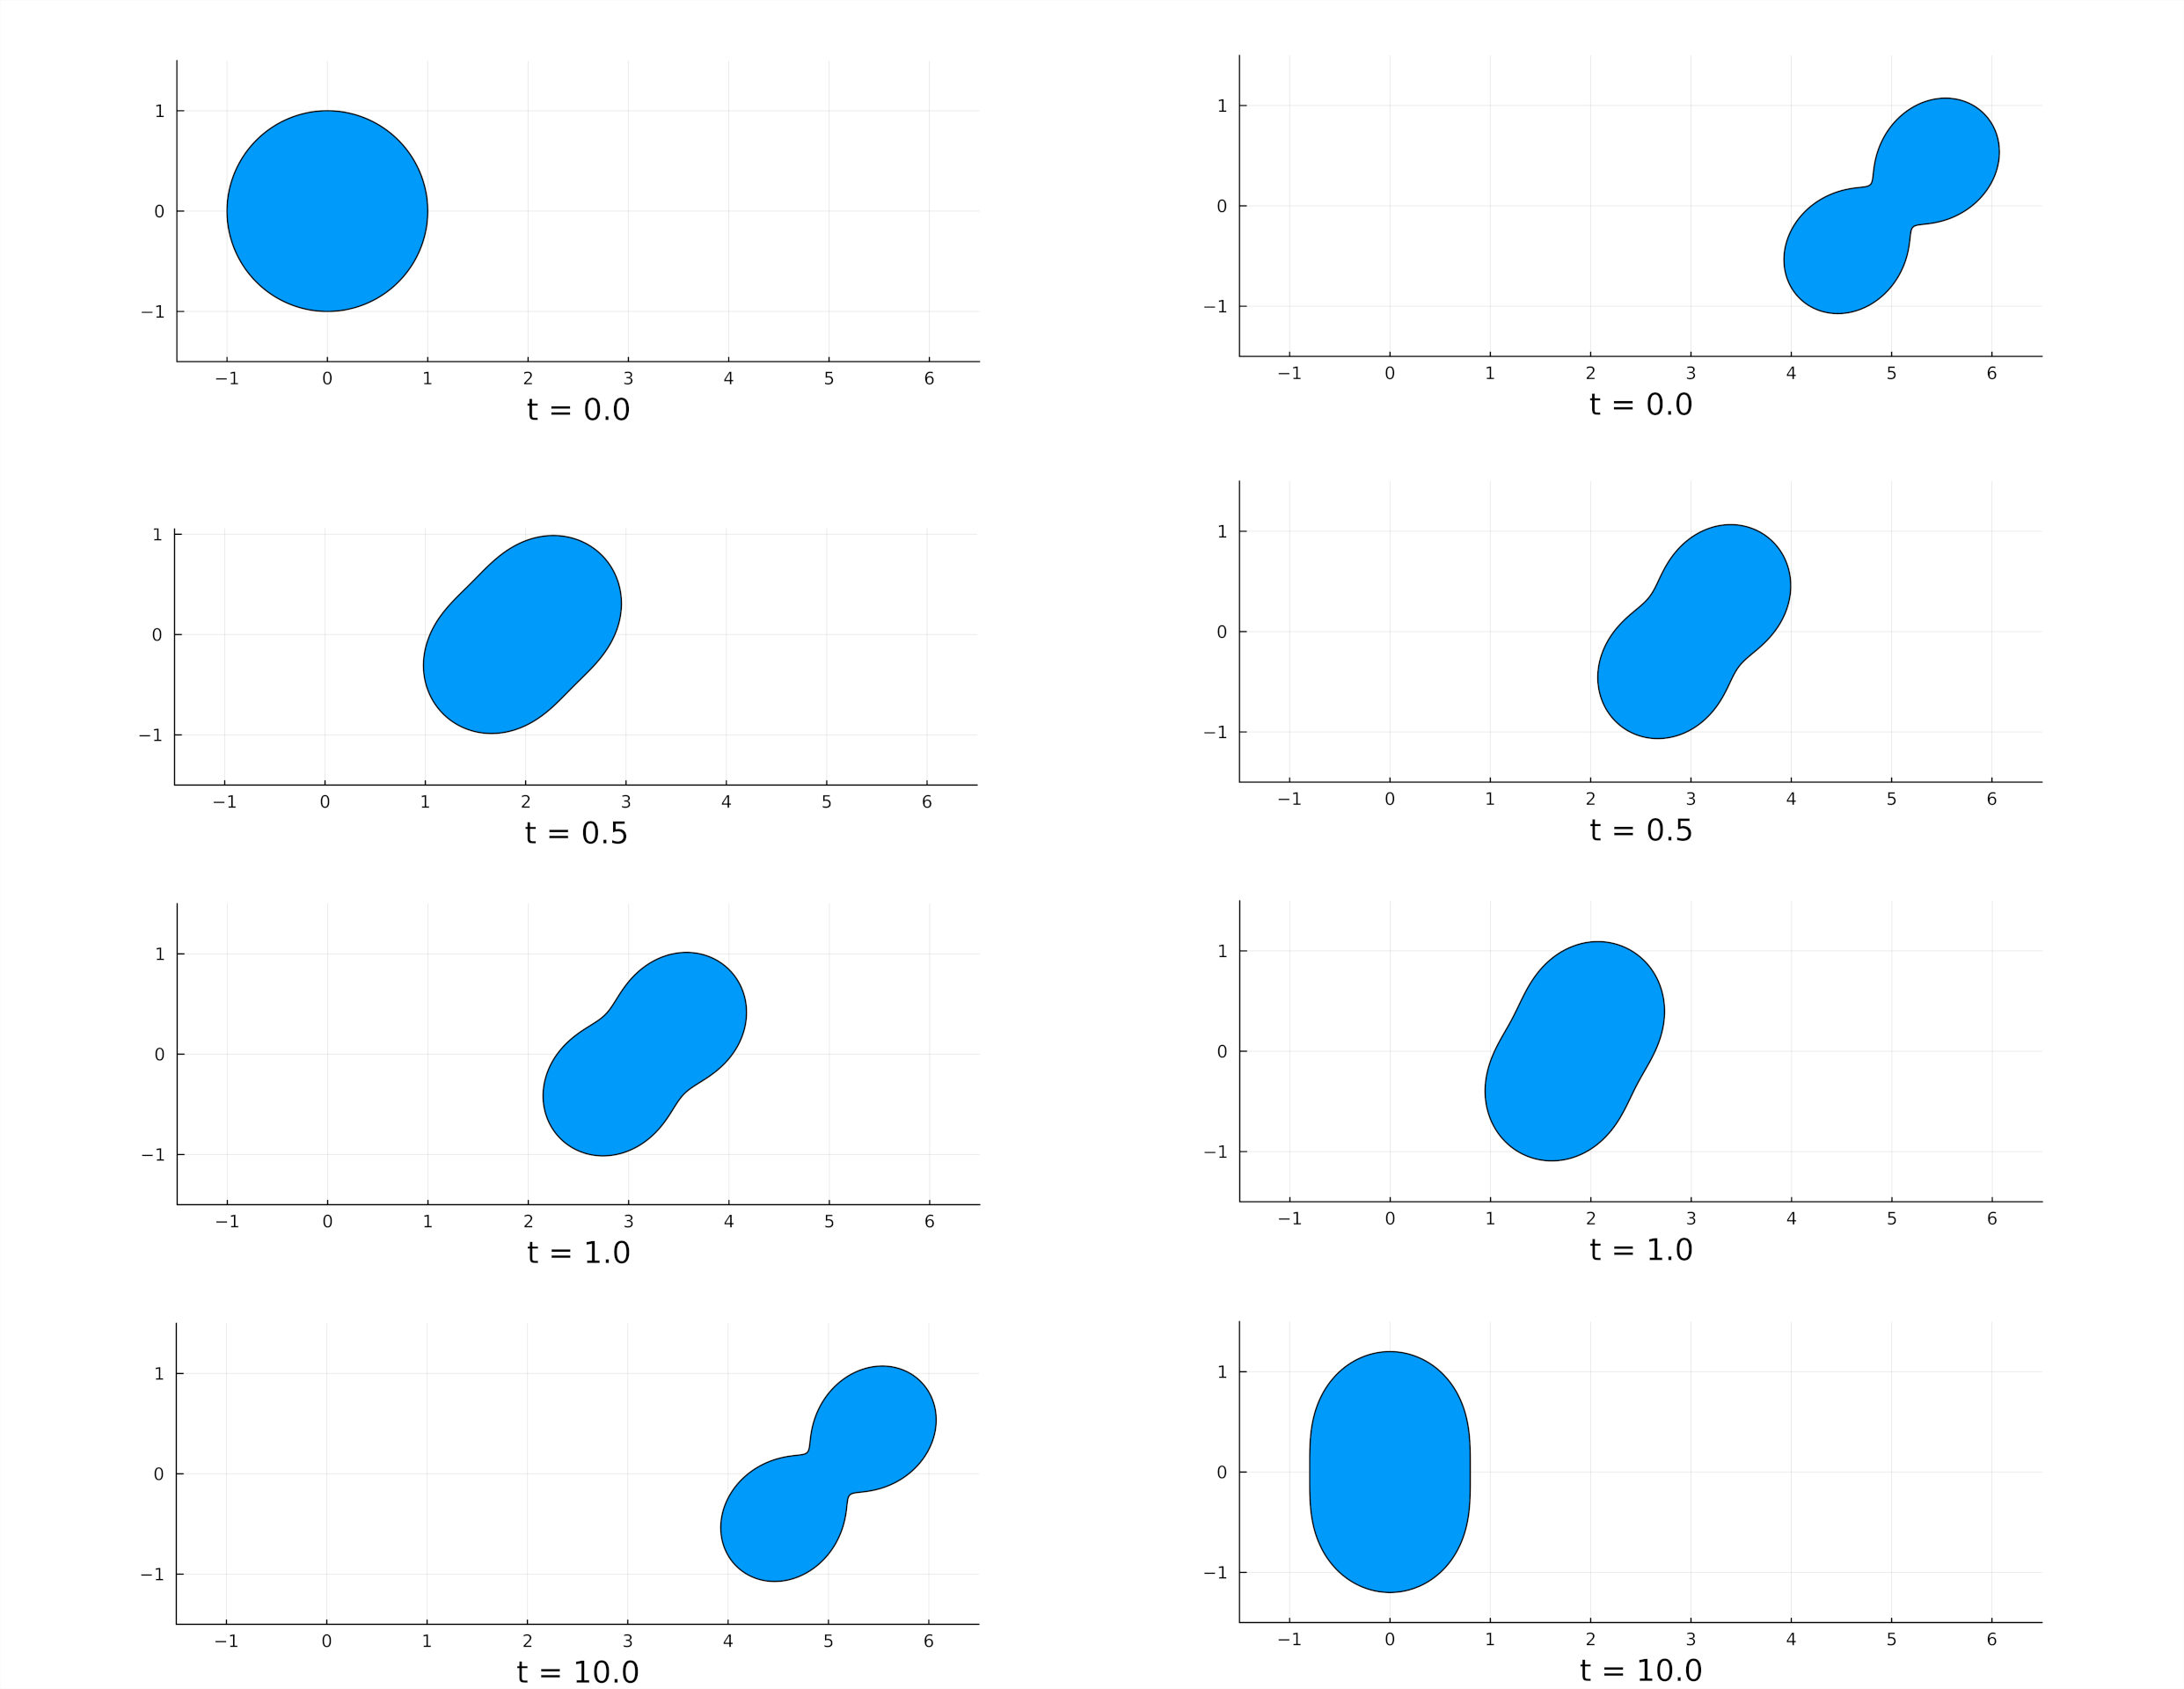
\includegraphics[width=16cm]{shape_resovery_example.png}
	\caption{Here, we can see two different cell developments associated with the shape recovery model. \\
	In the left column the initial state is given by the CRF cell $ C = ( (0, 0)^T, \phi \mapsto 1)$ and the desired state is $D = ( (5, 0)^T,  \phi \mapsto \frac{1}{2} \sin(2 \phi) + \frac{4}{5})$. \\
	The right column shows another transformation. The initial state is given by $D$ which is the desired state in the first column. The desired state in the right column is defined by the CRF $E = ((0, 0)^T, \phi \mapsto 1 - \frac{1}{5} \cos(2 \phi))$.}
	\label{fig:shapeRec}
\end{figure}
This is the first dynamic model. It is the only one in this thesis that is explicitly solved. The following systems become more complex and can no longer be solved explicitly. One advantage of an explicit solution is that one can calculate the solution straight away at any wanted time. Furthermore, no numerical approximation of the solution is required, which prevents many possible errors.



\newpage
\section{Energy based dynamics for the DF model} \label{sec:energyModels}
In the now following models, we want to take a look at a different approach. The next models are based on the application of energy functionalities on vertex models, similarly to a model that is explained in the paper [Fletcher et al., 2014]. We consider a set of $M$ DF cells, each with $N$ vertices. The vector $\vec{C} = ( C_1, \dots, C_M)^T$ holds all cells in the system where $C_i = (\vec{x}_{i1}, \ldots, \vec{x}_{iN})^T$ describes the vector of all vertices of the $i$th cell, $( 1 \leq i \leq M)$. As previously assumed, $\vec{x}_{N+1} := \vec{x}_{1}$.\\
An \textbf{energy function} is a mathematical function used in various fields, including physics, chemistry or material science. Its primary purpose in this thesis is to describe the potential energy associated with a single DF cell or a system of DF cells. We use energy functions to measure whether certain cell parameters, like area, edge lengths or interior angles have the right value. Each coming energy is identified by a capital Latin letter. \\
Once we have found an appropriate energy, we can then directly conclude a force which can get applied on the cells' vertices. \\
\begin{definition} \textbf{Force function} \label{def:forceFunction}\\
	For a given energy $E_i$ of the $i$th cell, the force $F_{j}^{(E_i)}$ that describes the impact of $E_i$ on the $j$th vertex of the $i$th cell is given by
	\begin{center}
		$F_{j}^{(E_i)}(\vec{C}) := -\alpha_{E_i}(\vec{C}) \nabla_{\vec{x}_{ij}} E_i(\vec{C})$,
	\end{center}
	where $\alpha_{E_i} > 0$ denotes a positive scaling factor and $\nabla_{\vec{x}_{ij}}$ is the gradient for the $j$th vertex of cell $i$. 	\\
\end{definition}
\begin{remark}\textbf{}\\
	Our energy functions have the structure $E = |$ desired state - current state $|$. For every coming force, we choose the value of the energy function as the scaling factor such that a high energy results in a stronger force. \\
	Another possible approach could be to write the energy functions in another form $E = \frac{1}{2} |$ desired state - current state $|^2$. Then, one would just have to compute the negative signed derivation of $E$ in order to get the same scaled force function as in the first approach, because of the chain rule. \\
	In both cases the energy $E$ would not be truly differentiable, because of the absolute value. However, we will use the derivative of $E$ to calculate the forces anyway, since the points at which $E$ is not differentiable form a null set.\\
\end{remark}
The application of these forces in a differential equation results in a so called gradient flow. This will lead to a deformation of the cell in such a way that the energy gets minimized. This corresponds to one of the most basic physical laws: For a closed system, with constant external parameters, the internal energy will decrease and approach a minimum value at equilibrium. 
To be able to implement the coming energies and forces, we must introduce the cells desired states. As the name suggests, the desired states are representative of the shape and size that a cell wants to develop into. The DF $C_i^{(d)}$ is the desired state of the $i$th cell in the system. 
In the following, we will derive different energy functions that will help our cell to develop to a desired cell state. 
To approximate the solutions to the differential equations, I used an Explicit Euler integrated in Julia, or an Euler Maruyama Scheme with a fixed step size of $\Delta t = 2^{-8}$. Thus, one time step in the coming figures is equivalent to a value of $2^{-8}$. \\
In some plots, one can see arrows reaching from the cell vertices into the domain. These arrows are exactly the from the algorithm computed forces that act at the specific vertex at that time in the simulation. 
 
\subsection{Area energy}
The first energy which we want to use is the area energy.
Other forces, that will get introduced afterwards, will usually lead to a reduction of the area. 
We want to ensure that the cell area remains almost constant over time. \\
We assume that all considered polygons have a positive orientation so that the shoelace formula can be applied. This is not a hard restriction, because all DF cells are positively orientated initially and the change from a negative orientated polygon into a positive orientated polygon is quite simple. The progress is already described at the end of Section \ref{sec:ImplementationDiscreteOverlap}. 
Fortunately, we have already derived a method to compute the current area of a positively orientated polygon in Section \ref{sec:CellDef}. Since every DF cell is also a polygon, we can just apply the shoelace formula to obtain
\begin{align}
	a(C_i(t)) :=  \frac{1}{2}\sum\limits_{j = 1}^{N} (x_{i,j}(t) y_{i,j+1}(t) - x_{i,j+1}(t) y_{i,j}(t)), \label{eq:areaOperator}
\end{align}
with $a \geq 0$ being the functional that maps a cell $C_i$ to its area and $\vec{x}_{i,j} = (x_{i,j}, y_{i,j})^T$ being the $j$th vertex of $C_i$.  
Since we want all of our cells to reach their desired states $C_i^{(d)}$, the desired cell area must be equal to the areas of the desired states. \\
Thus, we can save them as a vector 
\begin{center}
	$\vec{a}^{(d)} := ( a^{(d)}_1, \ldots, a^{(d)}_M )^T$, 
\end{center}
where $a^{(d)}_i = a(C_i^{(d)})$ denotes the area of  $C_i^{(d)}$, $(  1 \leq i \leq M)$. \\
\begin{definition} \textbf{Area energy} \\
	The energy $A_{i}$, used to keep the cell $i$ at a constant volume, reads 
	\begin{align}
		A_i(C_i) := | a^{(d)}_i - a(C_i) |. \label{eq:areaEnergy} 
	\end{align}
\end{definition}
This energy reaches its minimum value whenever $a^{(d)}_i = a(C_i)$. In order to derive the gradient flow for this energy, we must first compute its gradient. \\
\begin{proposition} \textbf{Area force} \\
	The gradient of $A_i$ with respect to the $j$th vertex of cell $i$ is given by 
	\begin{center}
		$\nabla_{\vec{x}_j} A_i(C_i) = \sgn(a(C_i) - a_i^{(d)}) \dfrac{1}{2} \begin{pmatrix} y_{i,j+1} - y_{i,j-1} \\ x_{i,j-1} - x_{i,j+1} \end{pmatrix}$. 
	\end{center}
	As a scaling factor, we choose
	\begin{center}
		$\alpha_{A_i}(C_i) := | a_i^{(d)} - a(C_i) |$. 
	\end{center}
	Thus, the area force reads 
	\begin{align}
		F_{j}^{(A_i)}(C_i) = \frac{1}{2}( a_i^{(d)} - a(C_i)) \begin{pmatrix} y_{i,j+1} - y_{i,j-1} \\ x_{i,j-1} - x_{i,j+1} \end{pmatrix}.
	\end{align}
	Proof.\\
	To reduce the notation effort, we neglect the subscript $i$, because we just consider a single cell.
	In order to compute $\nabla_{\vec{x}_j} | a^{(d)} - a(C) |$, let us first assume that $a^{(d)} \geq a(C)$. Then, one can calculate
	%\begin{itemize}		
	%	\item[] $\nabla_{\vec{x}_j} | a^{(d)} - a(C) | = - \nabla_{\vec{x}_j} a(C) = - %\frac{1}{2}\sum\limits_{j = 1}^{N} \nabla_{\vec{x}_j} (x_{j} y_{j+1} - x_{j+1} y_{j})$
	%	\item[$=$] $ - \frac{1}{2}\sum\limits_{j = 1}^{N} \begin{pmatrix} \partial_{x_j}  (x_{j} y_{j+1} - x_{j+1} y_{j})\\ \partial_{y_j} (x_{j} y_{j+1} - x_{j+1} y_{j})\end{pmatrix} = - \dfrac{1}{2} \begin{pmatrix} y_{j+1} - y_{j-1} \\ x_{j-1} - x_{j+1} \end{pmatrix}$
	%\end{itemize}
	\begin{center}
		$
		\nabla_{\vec{x}_j} | a^{(d)} - a(C) | = - \nabla_{\vec{x}_j} a(C)
		= - \frac{1}{2}\sum\limits_{j = 1}^{N} \nabla_{\vec{x}_j} (x_{j} y_{j+1} - x_{j+1} y_{j})$ \\ \smallskip 
		$=- \frac{1}{2}\sum\limits_{j = 1}^{N} \begin{pmatrix} \partial_{x_j}  (x_{j} y_{j+1} - x_{j+1} y_{j})\\ \partial_{y_j} (x_{j} y_{j+1} - x_{j+1} y_{j})\end{pmatrix} 
		= - \dfrac{1}{2} \begin{pmatrix} y_{j+1} - y_{j-1} \\ x_{j-1} - x_{j+1} \end{pmatrix}
		$
	\end{center}
	
	Remember that $a^{(d)}$ is just an independent constant. In the other case, where $a^{(d)} < a(C(t))$, there is just a change in the sign. The combination of both cases yields the expression above. \\ 
	Since $- | a^{(d)} - a(C) | \sgn(a(C) - a^{(d)}) = a^{(d)} - a(C)$, we can conclude the area force. \\
	\qed
\end{proposition}
For the computation of the gradient of the cell area, it is important that the cells has a positive orientation, i.e.the vertices must be ordered counterclockwise. For cells with a negative orientation, this formula will produce the wrong sign. \\ 
Having derived the area energy and force, we are ready to start the first simulations in order to see if the force does its job correctly. Therefor, we choose a setting with just one cell. \\
The initial condition is given by a regular hexagon. In the first simulation, the distances of each vertex to the centre will be 1 unit of length. This results the DF cell $ C(0) = ( (1, 0), (0.5, 0.87), (-0.5, 0.87), (-1.0, 0), (-0.5, -0.87), (0.5, -0.87))$ which can be seen in the first diagram of Figure \ref{fig:areaForce}
and in an initial cell area of $a(C(0)) = \frac{3 \sqrt{3}}{2} \approx 2.6$. 
As a desired cell area, we choose $a^{(d)} = 10$. Having dropped the index $i$ for the ease of notation, this results in the following ODE for each vertex.
\begin{model} \textbf{Area model} \label{model:area} \\
	The area model with $a^{(d)} = 10 $ is given by the IVP 
	\begin{center}
			$
			\begin{cases}
				\dfrac{d \vec{x}_j(t)}{d t} = F_{j}^{(A)}(C) =  \frac{1}{2}( 10 - a(C(t))) \begin{pmatrix} 		y_{j+1} - y_{j-1} \\ x_{j-1} - x_{j+1} \end{pmatrix}, \\
				\vec{x}_j(0) = \vec{x}_j^{\;(0)}, 
			\end{cases}
			$
	\end{center}
	with $\vec{x}_j^{\;(0)}$ being the $j$th vertex of $C(0)$.	
\end{model}
The result can be seen in Figure \ref{fig:areaForce}. Further models for different energies have the exact same structure and are therefor not written down explicitly. 
\begin{figure}[h!]
	\begin{center}
		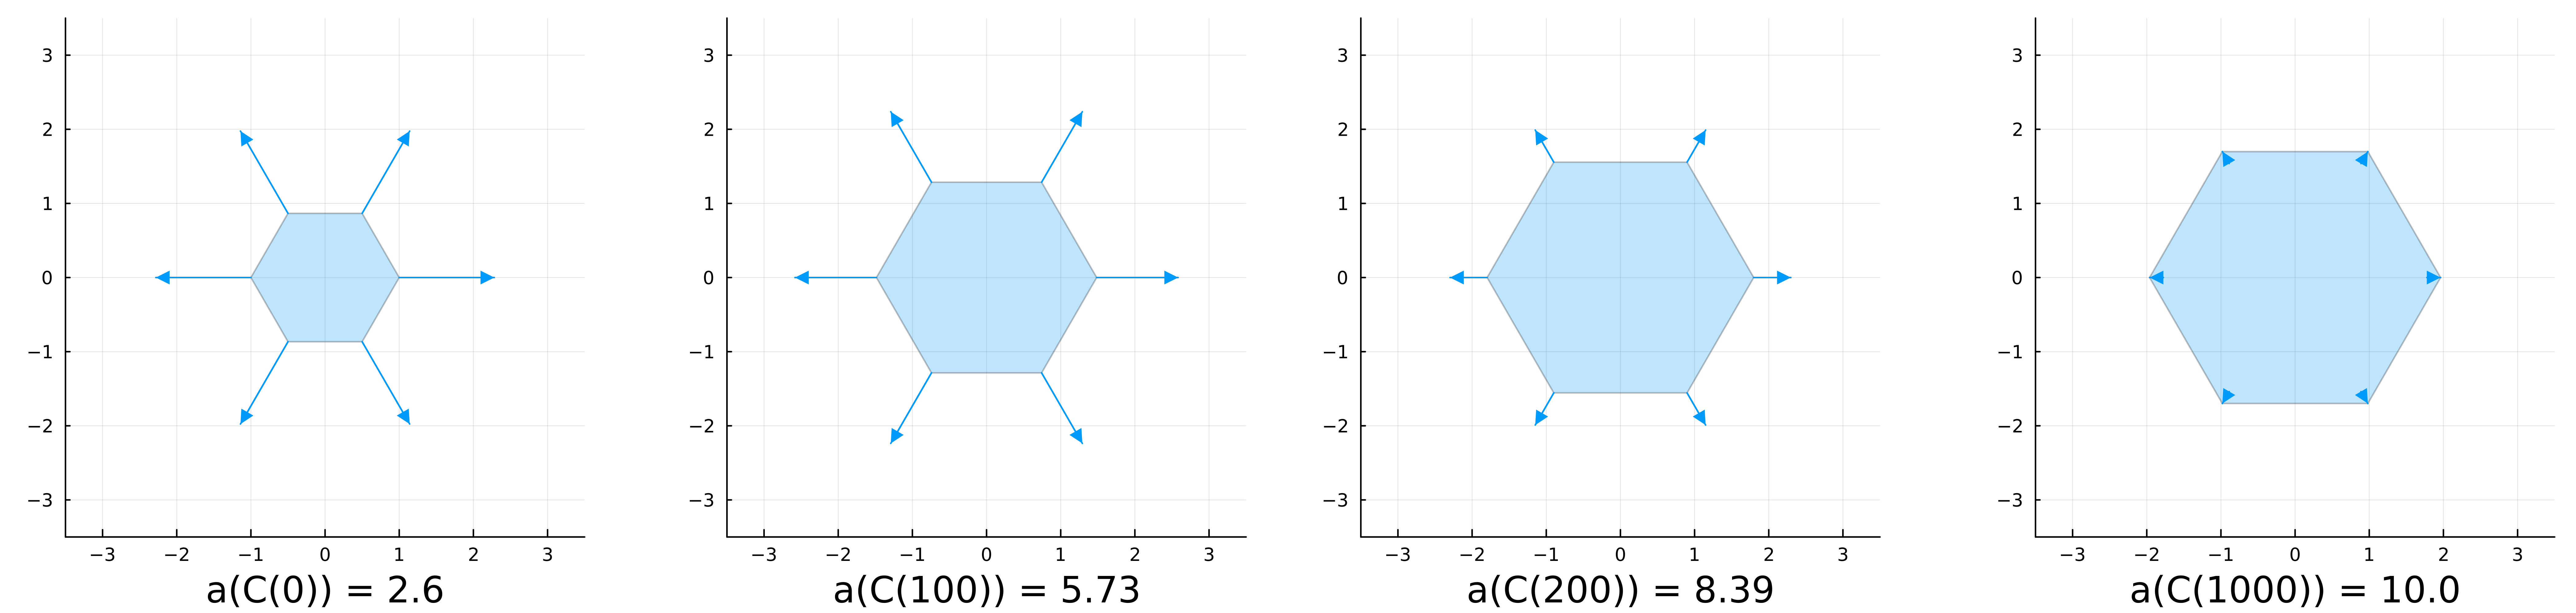
\includegraphics[width=15cm]{forces/area1/area1.png}
		\caption{This figure shows the solution at the times $t \in \{0, 100, 200, 1000\}$ to the Model \ref{model:area}, which uses the area force to bring the cell area to the desired state $a(C) = 10$. The cell has an initial  area of approximately $2.6$. The area force causes the vertices to move away from the cell centre, causing an increase of the cell area. The areas at the times shown can be seen under each diagram. One can see from the length of the arrows that the closer the current area gets to the desired state, the weaker the forces become. This corresponds to the scaling factor $|a^{(d)} - a(C)|$.	As soon as $a(C) = 10$, the forces stop acting and a steady state is reached.}
		\label{fig:areaForce}
	\end{center}
\end{figure}
As we can see, the area force works right if the current area is less than the desired area. Figure \ref{fig:areaForce2} shows a similar simulation, but with the difference that the cell area is initially larger than the desired cell area. Also this case works. 
\begin{figure}[h!]
	\begin{center}
		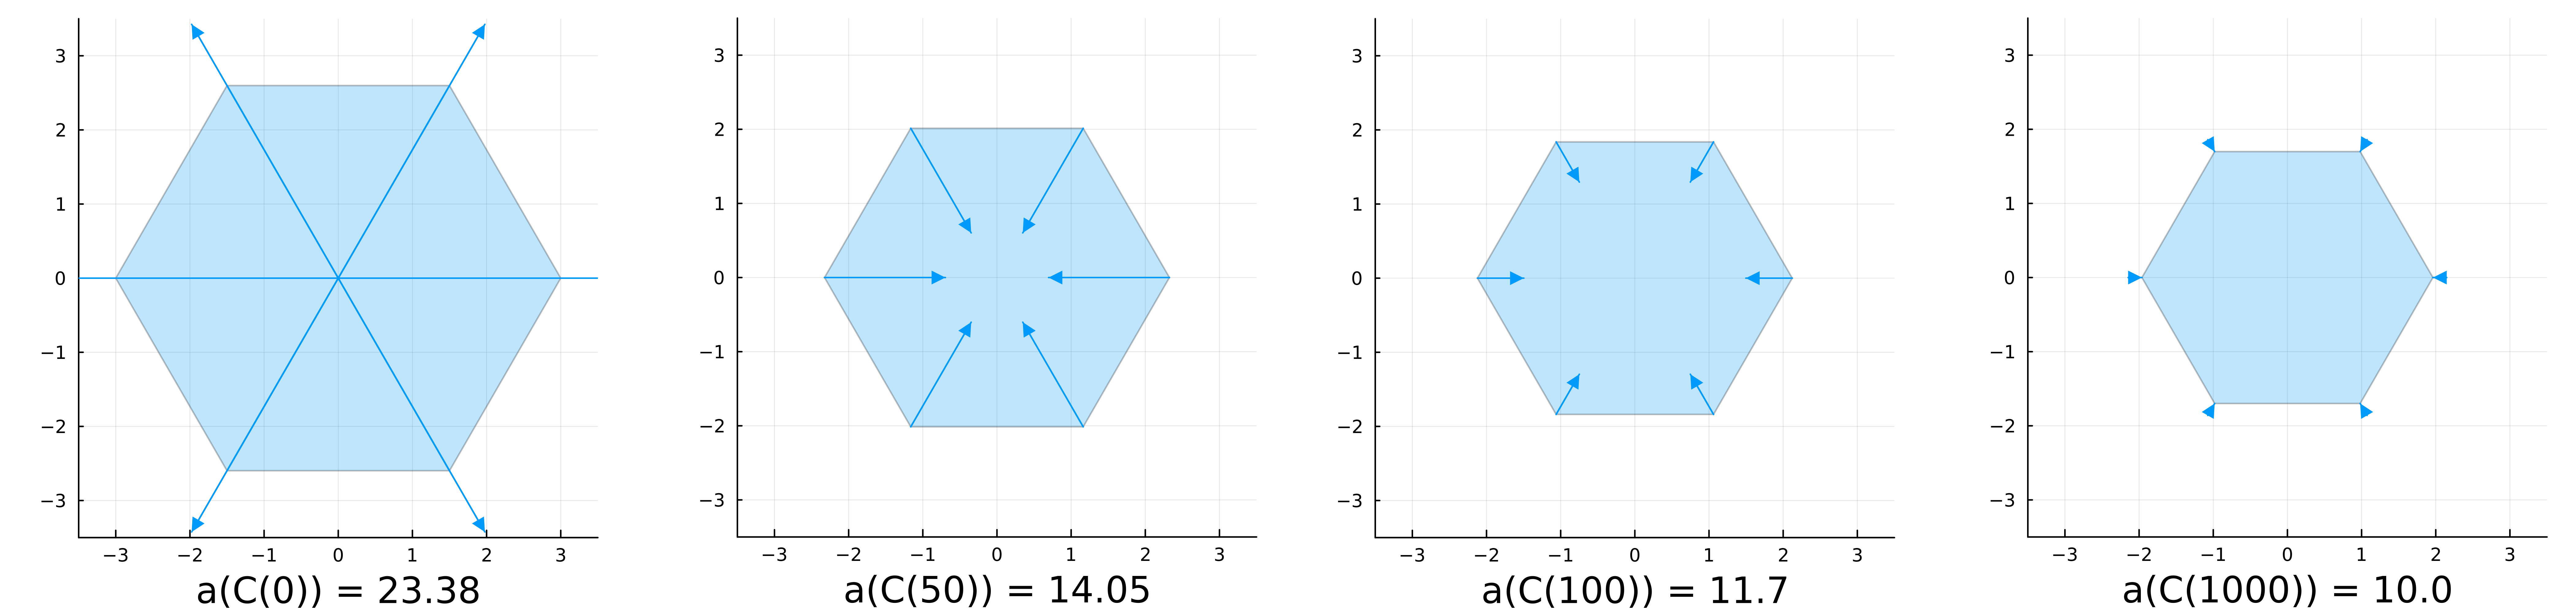
\includegraphics[width=15cm]{forces/area2/area2.png}
		\caption{Similar to Figure \ref{fig:areaForce}, this image shows a cell that develops according to the area force. In contrast to the last illustration, we assume an initial area of approximately 23.38. That means that the area force must act in the reversed direction in order to let the cell develop into the desired state $a^{(d)}=10$. As we can see in the four diagrams, this is exactly what happens. }
		\label{fig:areaForce2}
	\end{center}
\end{figure}

\subsection{Edge energy}  
We have already secured a constant cell area system. In the following two paragraphs, we want to focus on the cell developing into its desired shape. Our first step to ensure this, is the edge energy. Remember, that the edge between the vertices $j$ and $j+1$ is the $j$th edge. 
In a similar fashion to the area energy, we will use desired edge lengths $e^{(d)}_{ij} = \norm[ \vec{x}_{i,j} - \vec{x}_{i,j+1}]$. The functional that returns the edge length of edge $j$ is given by
\begin{align}
	e_j(C) := \norm[ \vec{x}_{j} - \vec{x}_{j+1} ].  
\end{align}
Having obtained this functional, we can introduce the edge energy. \\
\begin{definition} \textbf{Edge energy} \\ 
	The edge energy $E_{ij}$ for the $j$th edge of the $i$th cell reads
	\begin{align}
		E_{ij}(C_i) := | e^{(d)}_{i,j} -  e_j(C_i)|.
	\end{align}
\end{definition} 
The change of the position of the vertex $j$ will change the lengths of both edges $j-1$ and $j$. This results in a change in both energies $E_{i,j-1}$ and $E{i,j}$. Thus, we must consider these two energies in the edge force. \\
\begin{proposition} \textbf{Edge force} \\
	The edge force is given by the formula
	\begin{align}
		F^{(E_{ij})}_j(C_i) = \dfrac{e_{j-1} - e_{i, j-1}^{(d)}}{e_{j-1}(C_i) } \begin{pmatrix} x_{j-1} - x_j \\ y_{j-1} - y_j\end{pmatrix} + 
		\dfrac{e_{j} - e_{i, j}^{(d)}}{e_{j}(C_i)} \begin{pmatrix} x_{j+1} - x_j \\ y_{j+1} - y_j\end{pmatrix}.
	\end{align}
	We choose $\alpha_{E_{ij}} := | e_{ij}^{(d)} - e_j(C_i) |$. \\
	Proof. \\
	Since this force acts on each cell individually, we can neglect the subscript $i$.
	The searched term has the following structure
	\begin{center}
		$F^{(E_{j})}_j(C) = - \alpha_{E_{j-1}} \nabla_{\vec{x}_j} E_{j-1}(C) - \alpha_{E_{j}} \nabla_{\vec{x}_j} E_{j}(C)$,
	\end{center}
	with the scaling factors $\alpha_{E_j}$ already defined in the proposition. \\	
	The partial derivatives of the edge length $e_j$ are
	\begin{center}
		$\partial_{x_j} e_j(C) = \partial_{x_j} ( (x_{j+1}- x_j)^2 + (y_{j+1} - y_j)^2)^{\frac{1}{2}} = \dfrac{ x_j - x_{j+1} }{ e_j(C) }$, \\
		$\partial_{y_j} e_j(C) = \dfrac{ y_j - y_{j+1} }{ e_j(C) }$. \\
	\end{center}
	This yields
	\begin{center}
		$ \nabla_{\vec{x}_j} E_{j} = sgn(e_{j}^{(d)} - e_j(C)) \nabla_{\vec{x}_j} - e_j(C)  = sgn(e_{j}^{(d)} - e_j(C))  \dfrac{1}{  e_j(C) } \begin{pmatrix} x_{j+1} - x_j \\ 	y_{j+1} - y_j \end{pmatrix}$,
	\end{center}
	and analogously
	\begin{center}
		$\nabla_{\vec{x}_j} E_{j-1} = sgn(e_{j-1}^{(d)} - e_{j-1}(C_i))  \dfrac{1}{  e_{j-1}(C) } \begin{pmatrix} x_{j-1} - x_j \\ 	y_{j-1} - y_j \end{pmatrix}$. 
	\end{center}
	This yields the edge force 
	\begin{center}
		$F_j^{(E_{j})}(C) = \dfrac{e_{j-1}(C) - e_{j-1}^{(d)}}{e_{j-1}(C)} 
		\begin{pmatrix}  x_{j-1} - x_j \\ y_{j-1} - y_j  \end{pmatrix} + 
		\dfrac{e_{j}(C) - e_{j}^{(d)}}{e_{j}(C)} 
		\begin{pmatrix}  x_{j+1} - x_j \\ y_{j+1} - y_j  \end{pmatrix}$.
	\end{center}
	\qed  
\end{proposition}
The application of this force is illustrated in Figure \ref{fig:edgeForce}. For now, this is everything we want from the edge energy. We can conclude the edge model. 

\begin{figure}[h!]
	\begin{center}
		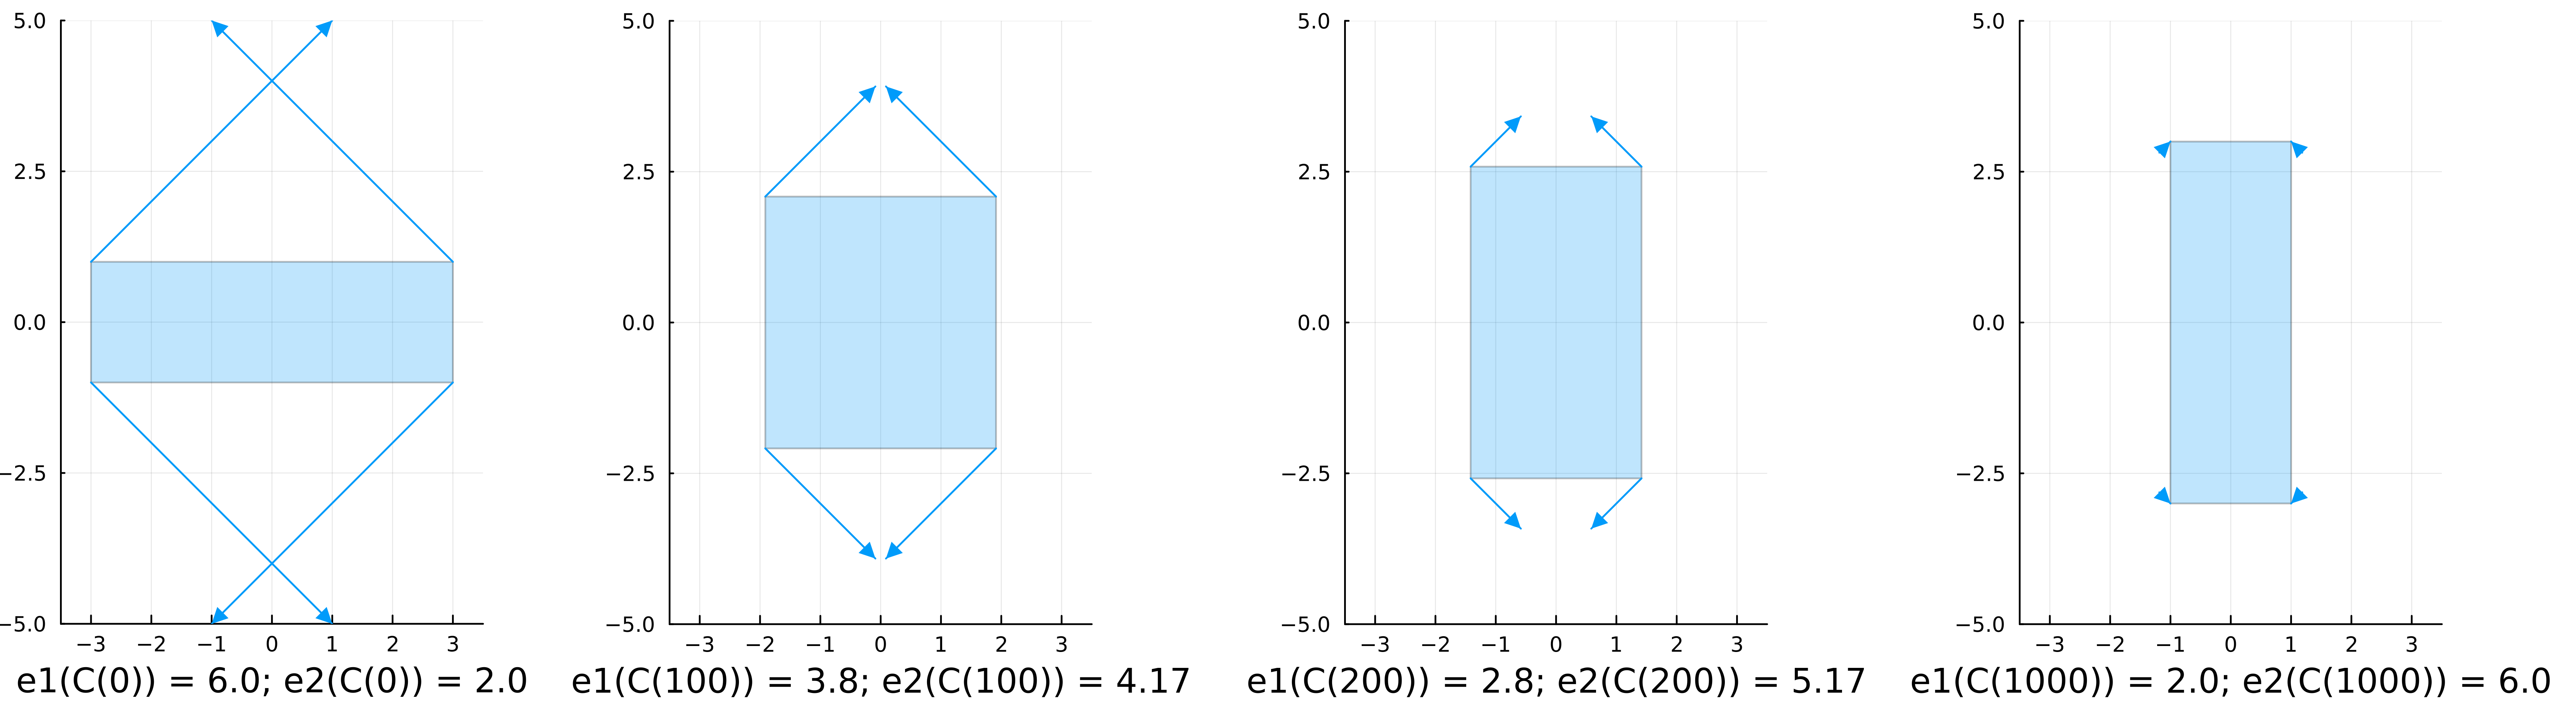
\includegraphics[width=15cm]{forces/edge/edge1.png}
		\caption{Here, we can see the edge force applied to a DF cell. At time $t=0$ the cell equals a rectangle $[-3, 3]\times[-1,1]$. Thus, the horizontal edges have a length of 6 and the vertical edges have a length of 2. These values at the according times $t \in \{ 0, 100, 200, 1000 \}$ are written under the diagrams. The desired state is equal to the rectangle $ [-1,1]\times[-3,3]$. That means that both horizontal edges must shrink and the vertical edges must expand. This behavior can be seen in the diagram sequence. }
		\label{fig:edgeForce}
	\end{center}
\end{figure}

\subsection{Interior angle energy}
In order to complete the shape recovery in our model, we will also concentrate on the now coming interior angle energy. As the name already tells, it is used to ensure that the interior angles at each vertex evolve into their desired states. Simulations without this energy sometimes lead to constrictions at certain vertexes where the interior angle goes to 360°. The interior angle energy shall also prevent this problem.\\
There are different ways to compute the angle that is given between two vectors. We choose the coming approach. \\
First of all, we want to be able to determine the angle $\theta$ between a given vector $\vec{v} = (v_1, v_2)^T$ and the $x$ axis. In the first and fourth quadrant, we can easily apply the $\arctan$ function to compute
\begin{center}
	$\theta = \arctan(\frac{v_2}{v_1})$. 
\end{center}
Unfortunately, it gets more complicated if $\vec{v}$ is located in the second or third quadrant. The usual $\arctan$ is not able to distinguish between these cases, because the fraction $\frac{v_2}{v_1}$ conceals the information of the signs of $v_1$ and $v_2$. However, there exists an extension of the common $\arctan$ function. It takes $v_1$ and $v_2$ as arguments and is hence able to make a case distinction for the different signs of the arguments. \\
\begin{definition} \textbf{arctan2} \\
	The function $$\atanxy:\R^2/\{0\} \rightarrow (-\pi, \pi],\: (x,y) \mapsto \atanxy(x,y)$$ computes the angle $\theta$ between $(x,y)^T$ and the $x$ axis. 
	\begin{center}
		$ \atanxy(x,y) = 
		\begin{cases}
			\arctan(\frac{y}{x}) & x > 0 \\
			\arctan(\frac{y}{x}) + \pi & x < 0, y > 0 \\
			\arctan(\frac{y}{x}) - \pi & x < 0, y < 0 \\
			\pi & x < 0, y = 0 \\
			\dfrac{\pi}{2} & x = 0, y > 0 \\ 		
			- \dfrac{\pi}{2} & x = 0, y < 0 \\ 
		\end{cases} $
	\end{center}
\end{definition}
This method provides high accuracy and robustness at all angles.\\
In order to obtain an interior angle at a certain vertex of a DF cell, we can use the interior angle functional.	\\
\begin{figure}[b!]
	\begin{center}
		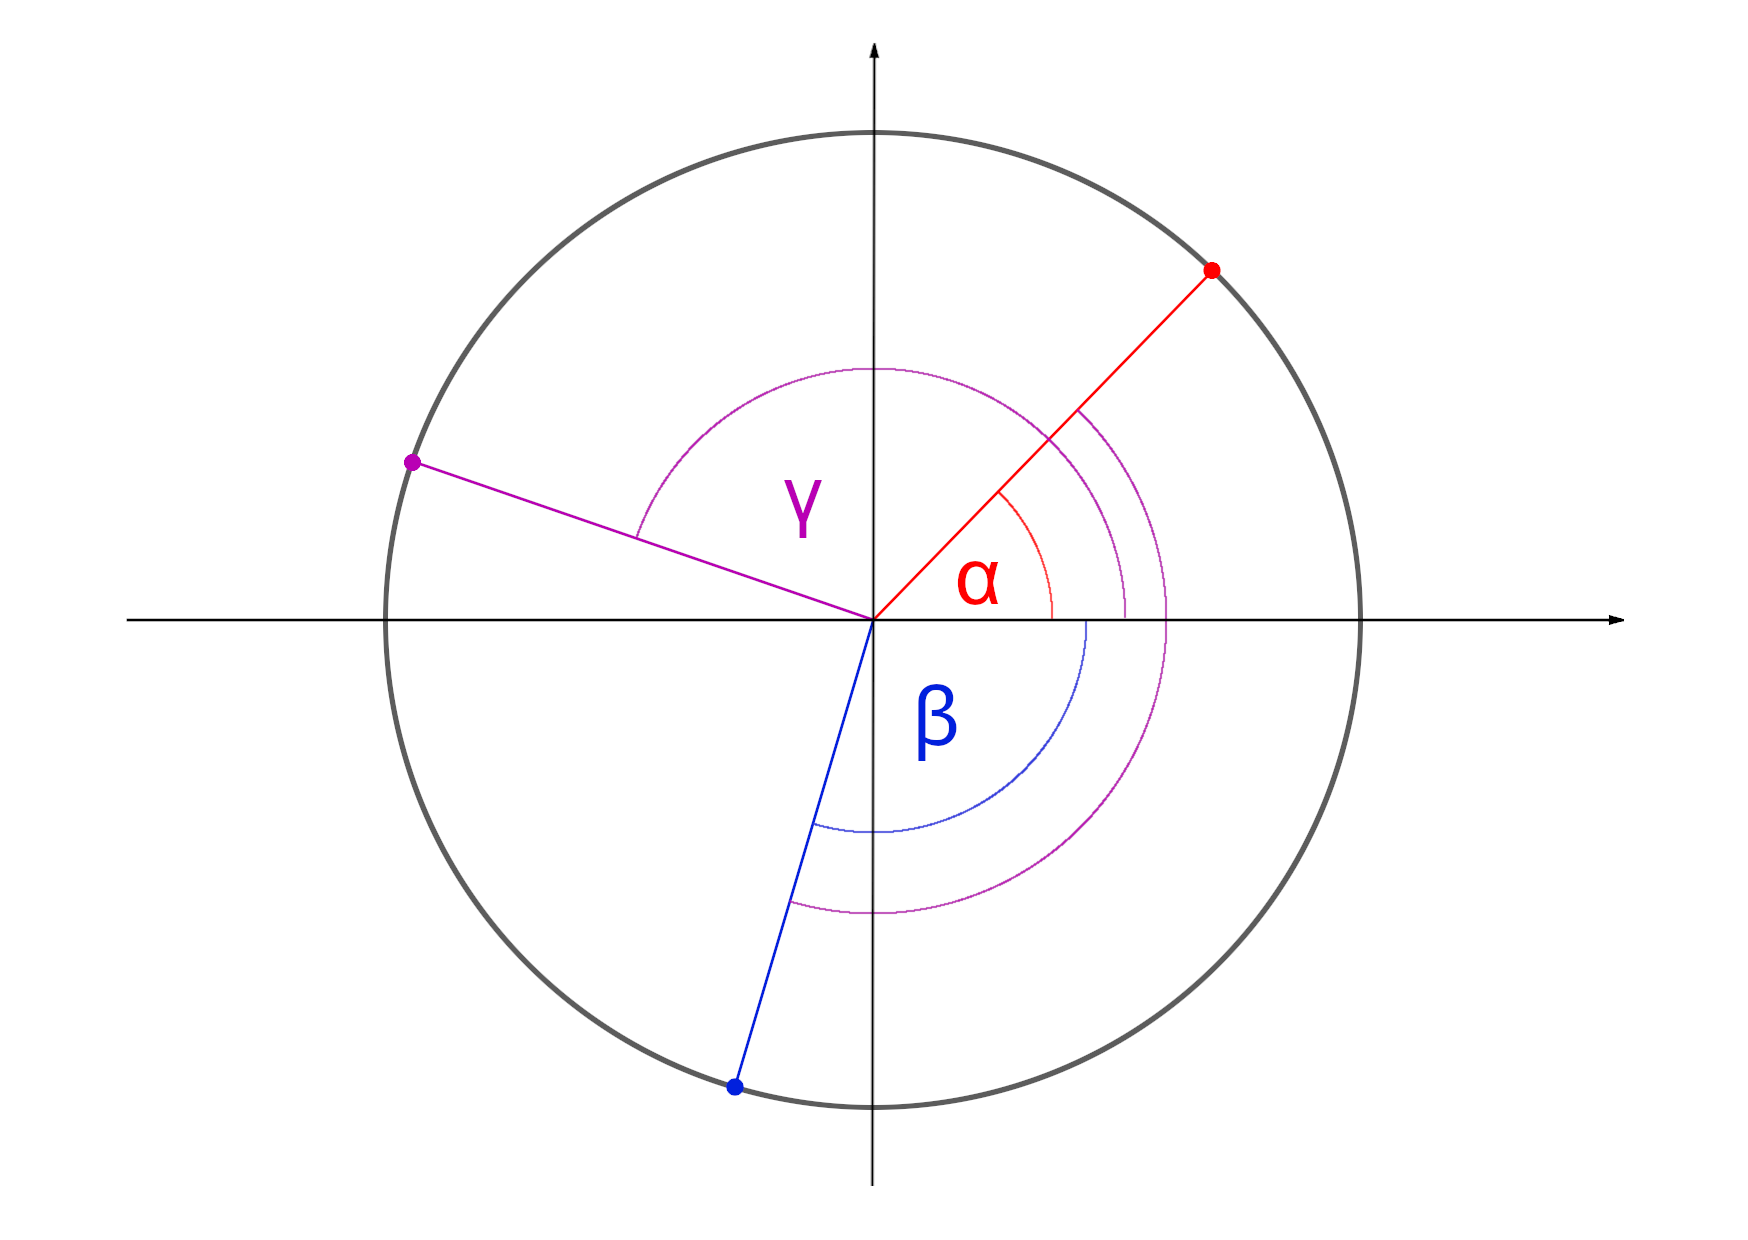
\includegraphics[width=8cm]{vectors.png}
		\caption{For two given vectors $\alpha \approx 45$° and $\beta \approx -115$°, we can apply the formula from the interior angle functional to compute $\gamma = [ 45$°$ - (-115$°$)]_{[0, 2\pi)} = 160$°, what is also the angle between $\alpha$ and $\beta$.}
		\label{fig:vectors}
	\end{center}
\end{figure}
\begin{definition} \textbf{Interior angle functional} \\
	The function $\iota_j(C_i)$ that computes the interior angle at vertex $j$ of cell $i$ is given by 
	\begin{align}
		\iota_j(C_i) := [\atanxy(\vec{v_1}) - \atanxy(\vec{v_2})]_{[0, 2\pi)},
	\end{align}
	where $\vec{v_1} := \vec{x}_{i,j-1} - \vec{x}_{i,j}$,  $\vec{v_2} := \vec{x}_{i,j+1} - \vec{x}_{i,j}$ and $[\: \cdot \: ]_{[0, 2\pi)}$ describes the modulo operator, that maps the argument into the interval $[0, 2\pi)$ by adding or subtracting $2\pi$ correspondingly often. \\
\end{definition}
Figure \ref{fig:vectors} illustrates the computation of the searched interior angle.	
In order to tell how each interior angle should evolve, we will again save the desired states $\iota_{ij}^{(d)} = \iota_j(C^{(d)}_i)$. \\
Then, we can write down the interior angle energy. \\
\begin{definition} \textbf{Interior angle energy} \\
	The interior angle energy $I_{ij}$ at vertex $j$ of cell $i$ is given by 
	\begin{align}
		I_{ij} := |\iota_{ij}^{(d)} - \iota_j(C_i)|.
	\end{align}
\end{definition}

\begin{proposition} \textbf{Interior angle force} \\
	The interior angle force is given by
	\begin{center}
		$F^{(I_{ij})}_j(C_i) = (\iota_{ij}^{(d)} - \iota_j(C_i))\left(
		\dfrac{1}{\norm[\vec{v}_1]^2} \begin{pmatrix}
			v_{1,y} \\-v_{1,x}
		\end{pmatrix}
		+ \dfrac{1}{\norm[\vec{v}_2]^2}\begin{pmatrix} -v_{2,y} \\ v_{2,x} \end{pmatrix}\right)
		$,
	\end{center}
	where $\vec{v}_1 = (v_{1,x}, v_{1,y})^T :=\vec{x}_{j-1} - \vec{x}_{j}$ and  $\vec{v}_2 = (v_{2,x}, v_{2,y})^T := \vec{x}_{j+1} - \vec{x}_{j}$. \\
	The scaling factor is defined as $\alpha_{I_{ij}} := | \iota_{ij}^{(d)} - \iota_j(C) |$. \\
	Proof. \\
	Again, we neglect the $i$, because we just consider one cell. 
	The goal is to determine the interior angle force
	\begin{center}
		$
		F^{(I_j)}_j(C) = - |\iota_{j}^{(d)} - \iota_j(C)| \nabla_{\vec{x}_j}I_j(C)
		$
	\end{center}
	Just like in the last forces, we use the $\sgn$ function to get rid of the absolute value, yielding
	\begin{center}
		$
		\nabla_{\vec{x}_j} I(C) = \sgn(\iota_j^{(d)}-\iota_j(C)) \nabla_{\vec{x}_j} (- \iota_j(C))
		$,
	\end{center}
	since the desired state is just a constant number. Since we have a minus in front of the gradient at the end of the equation, the searched force can be written as 
	\begin{center}
		$
		F^{(I_j)}_j(C) = (\iota_{j}^{(d)} - \iota_j(C)) \nabla_{\vec{x}_j}\iota_j(C)
		$.
	\end{center}
	The gradient of $\iota_j(C)$ is still missing. We will neglect the not differentiable modulo operator and must then compute
	\begin{center}
		$
		\nabla_{\vec{x}_j} (\atanxy(\vec{v}_1(C)) - \atanxy(\vec{v}_2(C))), 
		$
	\end{center}
	where $\vec{v}_1(C) = (x_{j-1} - x_{j} , y_{j-1} - y_{j})^T$ and $\vec{v}_2(C) = (x_{j+1} - x_{j} , y_{j+1} - y_{j})^T$. \\
	The function $\atanxy$ is partly defined and not truly differentiable. We still want to compute a gradient to use it for our interior angle force. Since $\atanxy(x,y) = \arctan(\frac{y}{x}) + \; constant$ almost everywhere, we will use the function $g(x,y) = \arctan(\frac{y}{x})$ for the derivation, because the different constants do not matter in the derivation. With $g$, we can rewrite $\iota_j(C) =g(x,y) \circ \vec{v}_1(C) - g(x,y) \circ \vec{v}_2(C) $. \\
	Thus, we need to determine 
	\begin{center}
		$
		\nabla_{\vec{x}_j} (g(x,y) \circ \vec{v}_1(C) - g(x,y) \circ \vec{v}_2(C)).
		$
	\end{center}
	The partial derivatives of $g$ are
	\begin{center}
		$\partial_{x} \arctan(\frac{y}{x}) = - \dfrac{y}{x^2} \dfrac{1}{1 + (\frac{y}{x})^2} = - \dfrac{y}{x^2 + y^2}$, \\
		$\partial_{y} \arctan(\frac{y}{x}) =  \dfrac{1}{x} \dfrac{1}{1 + (\frac{y}{x})^2} =  \dfrac{x}{x^2 + y^2}$.
	\end{center}
	It is easy to see that 
	\begin{center}
		$
		\partial_{x_j} \vec{v}_1(C) = \partial_{x_j} \vec{v}_2(C) = (-1,0)^T,
		\partial_{y_j} \vec{v}_1(C) = \partial_{y_j} \vec{v}_2(C) = (0, -1)^T. 
		$
	\end{center}
	This implies
	\begin{figure}[b!]
		\begin{center}
			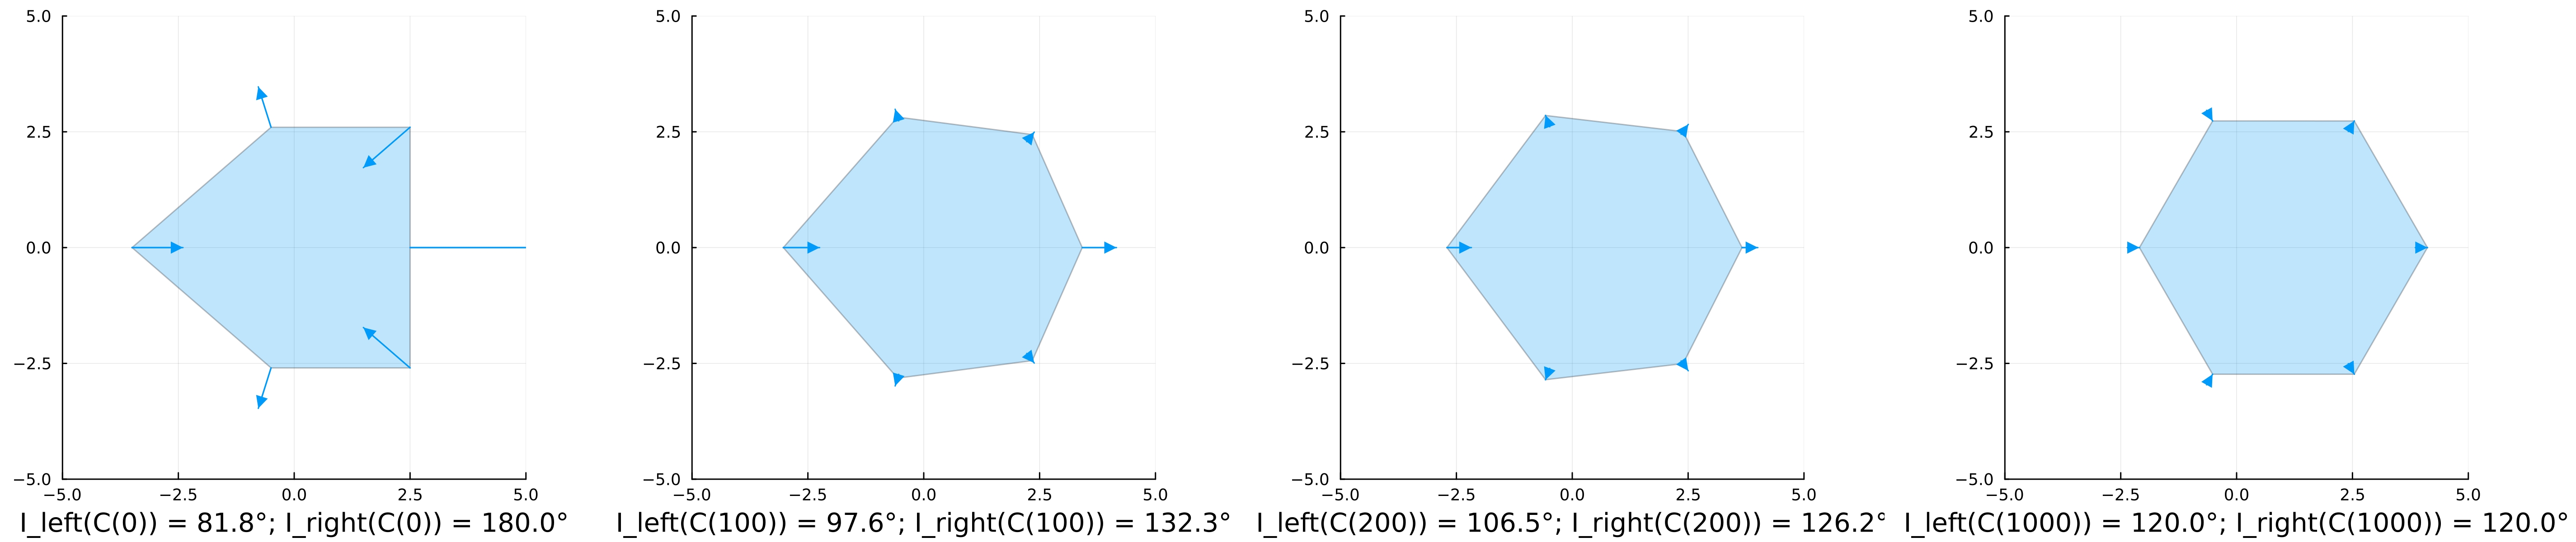
\includegraphics[width=15cm]{forces/angle/angle1.png}
			\caption{This figure shows how the interior angle force acts on the vertices of a DF cell. The initial state can be seen in the first diagram. The desired state is the horizontally mirrored version of the initial state. Below each chart, we can see the current interior angles at $t \in \{0,50,100,3000\}$ of the two vertices that have the $y$ value zero. The desired states are $90$° for the right and $270$° for the left considered vertex. The interior angle force ensures that each interior angle transitions to the desired state over time, as we can see in this figure. }
			\label{fig:angleForce}
		\end{center}
	\end{figure}
	\begin{center}
		$
		\partial_{x_j} \iota_j(C) 
		\corresponds \partial_{x_j}( g\circ \vec{v}_1(C) - g \circ \vec{v}_2(C))$ \\ \smallbreak	
		$= (g'(\vec{v}_1(C)) \partial_{x_j} \vec{v}_1(C) - g'(\vec{v}_2(C))\partial_{x_j} \vec{v}_2(C) $ \\ \smallbreak	
		$= -(\partial_x g)(\vec{v}_1(C)) + (\partial_x g)(\vec{v}_2(C))$\\ \smallbreak 
		$= \dfrac{ v_{1,y} }{ v_{1,x}^2 + v_{1,y}^2 } - \dfrac{v_{2,y}}{v_{2,x}^2 + v_{2,y}^2}
		$,
	\end{center}
	using the multidimensional chain rule. In a similar fashion, we obtain
	\begin{center}
		$
		\partial_{y_j} \iota_j(C) = -\dfrac{v_{1,x}}{v_{1,x}^2 + v_{1,y}^2} + \dfrac{v_{2,x}}{v_{2,x}^2 + v_{2,y}^2}.
		$
	\end{center}
	Together this yields
	\begin{center}
		$
		\nabla_{\vec{x}_j} \iota_j(C) = \dfrac{1}{\norm[\vec{v}_1]^2} \begin{pmatrix} v_{1,y} \\ - v_{1,x} \end{pmatrix} + 
		\dfrac{1}{\norm[\vec{v}_2]^2} \begin{pmatrix} -v_{2,y} \\ v_{2,x} \end{pmatrix},
		$
	\end{center}
	which corresponds to the term from the proposition.\\
	\qed 
\end{proposition}

As in the last two paragraphs, we can see the effect of $F^{(I_{ij})}_j(C)$ in an example in Figure \ref{fig:angleForce}.
The interplay between the edge- and inter angle forces result in a quite nice ability of the cell to develop into the desired cell shape. Figure \ref{fig:shapeShifteros} in Subsection \ref{par:shapeRecovery} illustrates this quite well.  

\subsection{Overlap energy}  \label{sec:overlapEnergy} 
While all previous energies are operating on each cell individually, the overlap energy is the first one that considers multiple cells and thus, adds the first cell interaction into the simulation. The overlap energy has quite a lot of similarities to the area energy, since in both cases the goal is to achieve a certain cell area. \\
But in difference to the area energy, it is not a cell from the considered system $\vec{C}$ whose area gets optimized, but new DF cells that are exactly equal to the overlap that occurs between two cells $C_i, C_j \in \vec{C}$. The new DF cells in the set of all overlaps between the original cells $C_i$ and $C_j$ $\Omega_{ij} = (D_1, \ldots, D_{k_j})$ fulfil the relation 
\begin{center}
	$
	C_i \cap C_j = \amalg_{k=1}^{k_j} D_k
	$,
\end{center}
where $\amalg$ symbolises a disjointed union and $k_j$ denotes the number of overlaps that occur between $C_i$ and $C_j$. As already explained in Section \ref{sec:CellDef}, every overlap that appears between two cells $C_i$ and $C_j$ can be nicely expressed through a new DF. Every vertex from an overlap cell is either included in $C_i$, $C_j$ or in the set $I_{ij}$ that holds all intersection points of $C_i$ and $C_j$. The determination of those overlap cells is also derived Section \ref{sec:CellDef}. 
Having all requirements stated, we can now introduce the overlap energy. \\
\begin{definition} \textbf{Overlap energy} \\
	Let $C_i$ and $C_j$ be two cells from the system $\vec{C}$ and $\Omega_{ij}$ be the set of all overlap DF that appear between $C_i$ and $C_j$, like explained above. Then, the overlap energy of $C_i$ is given by the formula 
	\begin{align}
		O_i(\vec{C}) := \sum\limits_{j=1 , j \neq i}^{M} (\sum\limits_{D_j \in \Omega_{ij}} a(D_j)),		
	\end{align} 
	where $a$ is the area functional \eqref{eq:areaOperator}. \\
\end{definition}
The first sum iterates over all other cells in the system, while the second sum iterates over all overlaps that occur between both cells. We do not need an absolute value, because the area functional $a$ always computes non negative values. \\
An important assumption for the overlap force is that the vertices $\vec{x}_{ij}$ of $C_i$ that are also included in the overlap $D$ are identified with the according vertices in $D$. Let $\omega_{ik} = C_i \cap D_k$ be the set of the vertices that are in $C_i = (\vec{x}_{i1}, \ldots, \vec{x}_{iN})$ and $D_k = (\vec{d}_{k1}, \ldots, \vec{d}_{kL})$. Then, we can find an overlap vertex $\vec{d}_l$ that corresponds to $\vec{x}_j$, whenever $\vec{x}_j \in \omega_{ik}$. In the computation for the overlap force, we can then use $\nabla_{\vec{d}_l} a(D_k)$.\\
If a vertex $\vec{x}_{ij}$ is not part of the overlap $D_k$ then this overlap will not have an impact on this vertex. \\
\begin{proposition} \textbf{Overlap force} \\
	 The overlap force $F_j^{(O_i)}$ that acts on $\vec{x}_{ij}$ is given by
	\begin{align}
		F_j^{(O_i)}(\vec{C}) = \sum\limits_{m=1, m\neq i}^{M} ( \sum\limits_{D_k \in \Omega_{im}} - \mathbbm{1}_{\omega_{ik}}(\vec{x}_{ij})  a(D_k)\nabla_{\vec{d}_{l}} a(D_k)),
	\end{align}
	with $\nabla_{\vec{d}_{l}} a(D_k)$ given as
	\begin{center}
		$\nabla_{\vec{d}_{l}} a(D_k) = 
			\dfrac{1}{2}\begin{pmatrix}	d_{l+1}^{y} - d_{l-1}^{y} \\d_{l-1}^{x} - d_{l+1}^{x}	\end{pmatrix},
		$
	\end{center}
	with $\vec{d}_{l}$ being the corresponding vertex to $\vec{x}_{ij}$ in the according overlap and $\vec{d}_{l-1}$ and $\vec{d}_{l+1}$ being the vertices before and after $\vec{d}_{l}$. \\
	Proof. \\
	Instead of just using one scaling factor for each vertex, we will use a scaling factor $\alpha_{O_i, D_k} = a(D_k)$ for each individual overlap $D_k$. \\
	For all vertices $\vec{x}_{ij} \notin \omega_{ik}$, that are not included in the overlap $D_k$, the force is zero, because a change of position would not impact the area of the overlap in this case. This produces the indicator function $\mathbbm{1}_{\omega_{ik}}(\vec{x}_{ij})$ in the formula, that makes the force vanish for $\vec{x}_{ij} \notin \omega_{ik}$. \\
	Per definition of $\omega_{ik}$, we can always find an overlap vertex $\vec{d}_l$ that corresponds to $\vec{x}_{ij}$ if $\vec{x}_{ij} \in \omega_{ik}$. In this case, we can apply the gradient with respect to $\vec{d}_l$ on the area functional of $D_k$, to compute the direction of the fastest descent. \\	
	Thus, we must solve 
	\begin{center}
		$
		F_j^{(O_i)}(\vec{C}) = \sum\limits_{l=1, l\neq i}^{M} ( \sum\limits_{D_k \in \Omega_{il}} -\mathbbm{1}_{\omega_{ik}}(\vec{x}_{ij}) a(D_k) \nabla_{\vec{d}_l} a(D_k)).
		$
	\end{center}
	We can use the gradient computation shown in the area force, to determine
	\begin{center}
		$
		\nabla_{\vec{d}_l} a(D_k) = \frac{1}{2} 
		\begin{pmatrix}	d_{l+1}^{y} - d_{l-1}^{y} \\d_{l-1}^{x} - d_{l+1}^{x}	\end{pmatrix}
		$.
	\end{center}
	\qed
\end{proposition}
In order to compute the gradient correctly, it is necessary that the overlap cell has a positive orientation. Otherwise, we would get a wrong sign, because $\vec{d}_{j-1}$ and $\vec{d}_{j+1}$ would be swapped. But this is also guarantied in the computation of the overlap. \\ 
Figure \ref{fig:overlapForce} shows the cell interaction between two overlapping cells with the overlap force acting on the vertices. 
\begin{figure}[h!]
	\begin{center}
		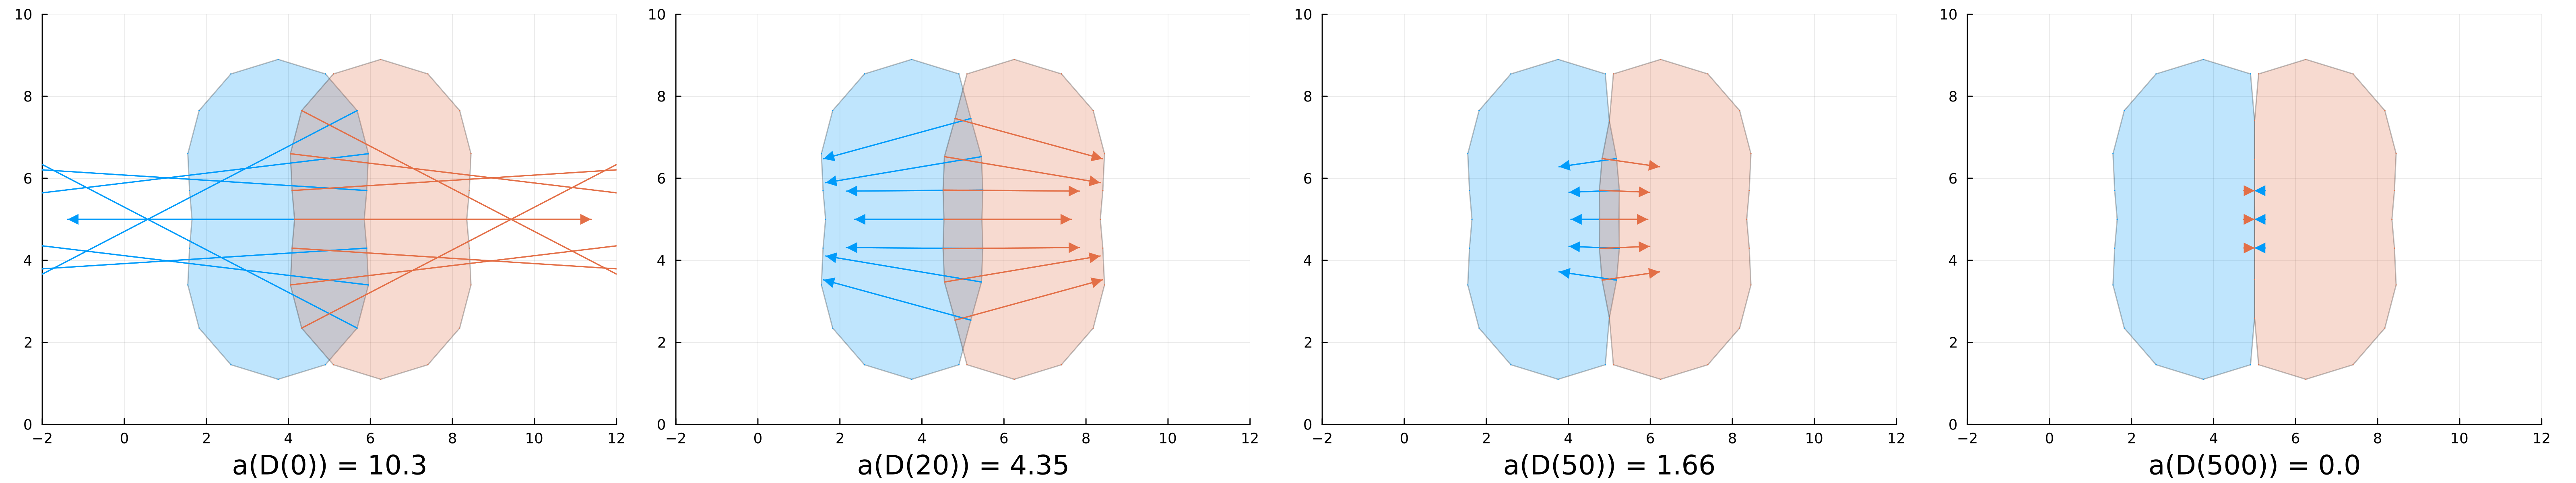
\includegraphics[width=15cm]{forces/overlap/overlap1.png}
		\caption{Here, we can see how the overlap force acts on two overlapping DF cells. The blue arrows represent the forces acting on the blue cell, the red arrows the forces of the red cell. The cells are shown at the times $t \in \{0, 20, 50, 500\}$, as well as the current area of the cell overlap $D$. On each consecutive diagram, we can see that the overlap gets reduced, until the area of the overlap is zero at $t=500$.  }
		\label{fig:overlapForce}
	\end{center}
\end{figure}

\subsection{Discrete shape recovery} \label{par:shapeRecovery} 
We have now introduced all the forces that we want to use in this thesis. The next step is to combine the forces to see how the interactions between the forces affect the cell developments. \\
First, let us take a look at the first three forces, that shall make the cell develop into a certain desired state. Since these forces act on each cell separately, it is sufficient to consider a single DF cell. \\
In order to make it quite difficult for the forces to ensure the desired state, we choose a desired state, that has a completely different shape than the initial cell. Both states are shown in Figure \ref{fig:shaperrrs}. \\
\begin{figure}[h!]
	\centering
	\centering
	\begin{subfigure}{0.4\textwidth}
		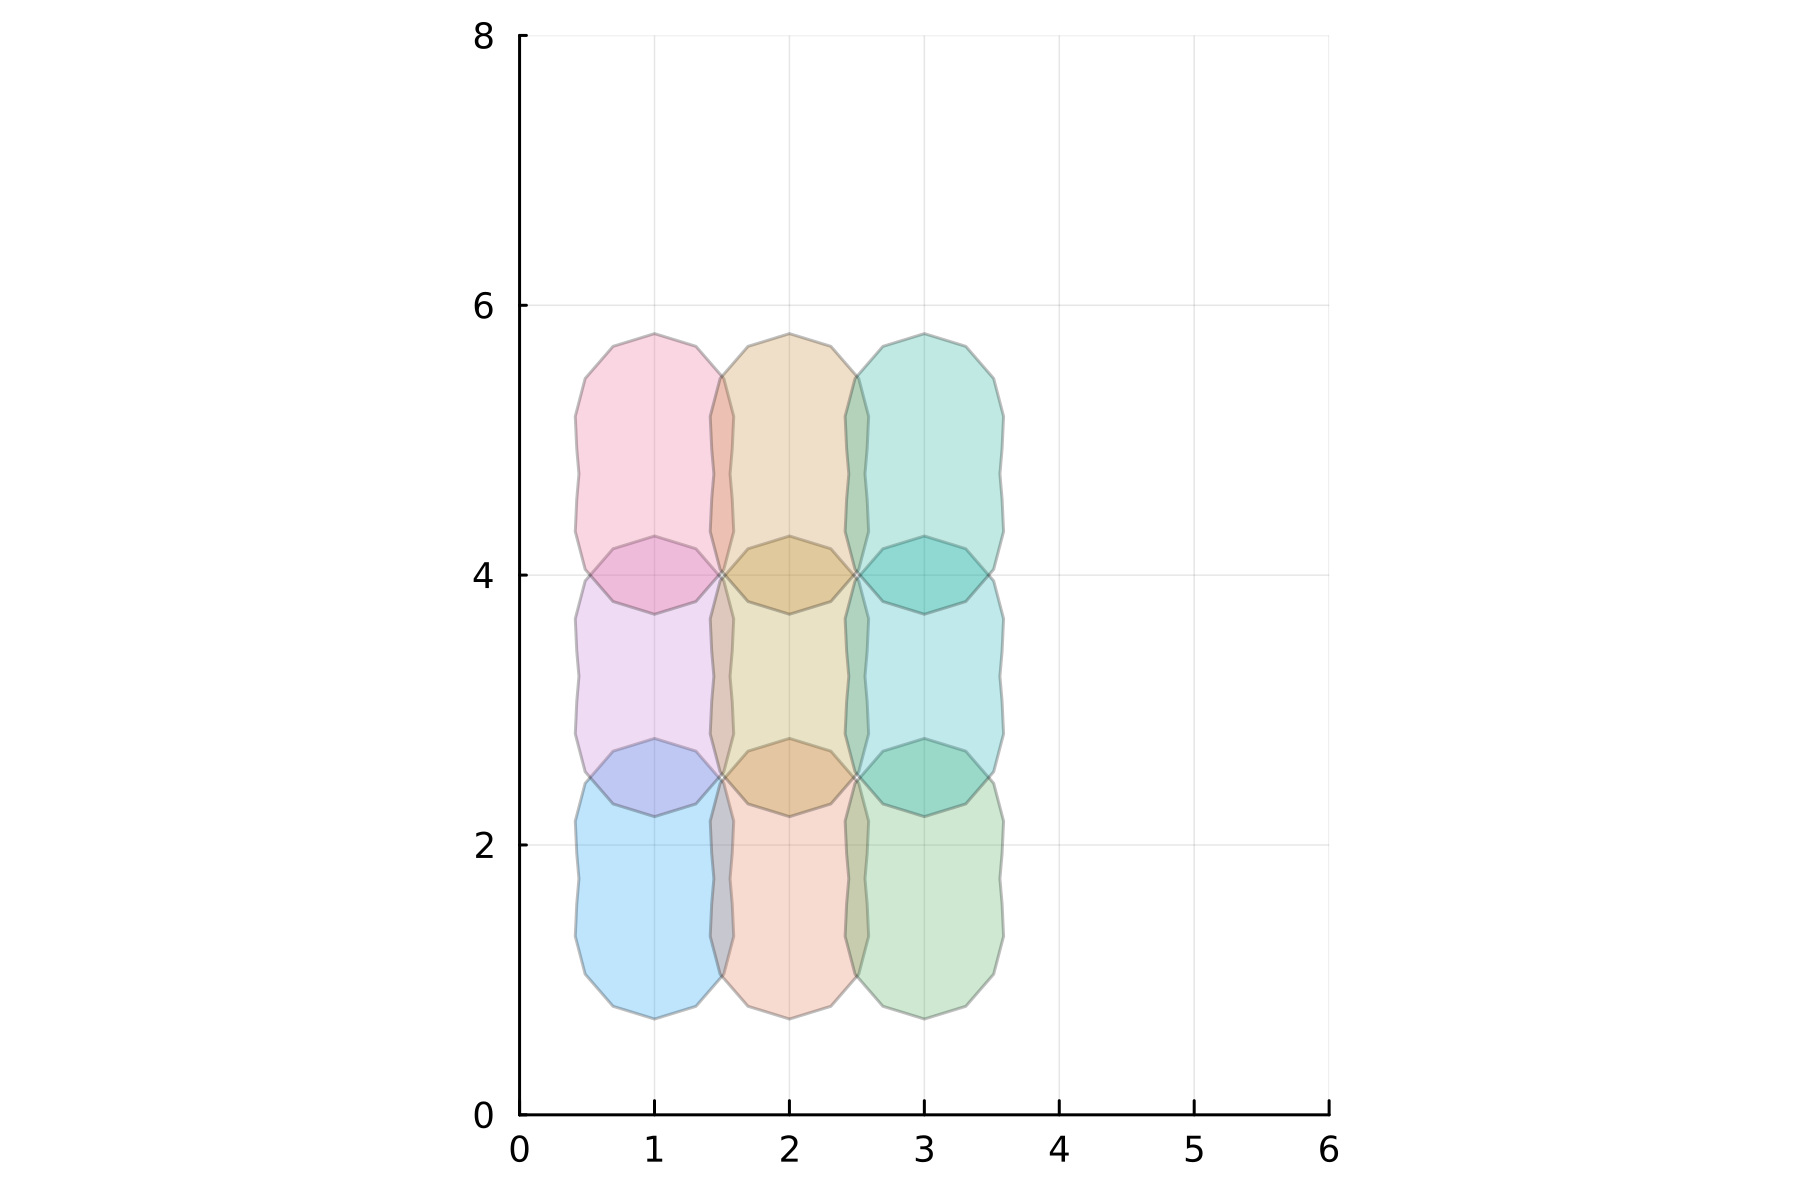
\includegraphics[width=\textwidth]{forces/shapes/initial.png}
		
	\end{subfigure}
	\hfill
	\begin{subfigure}{0.4\textwidth}
		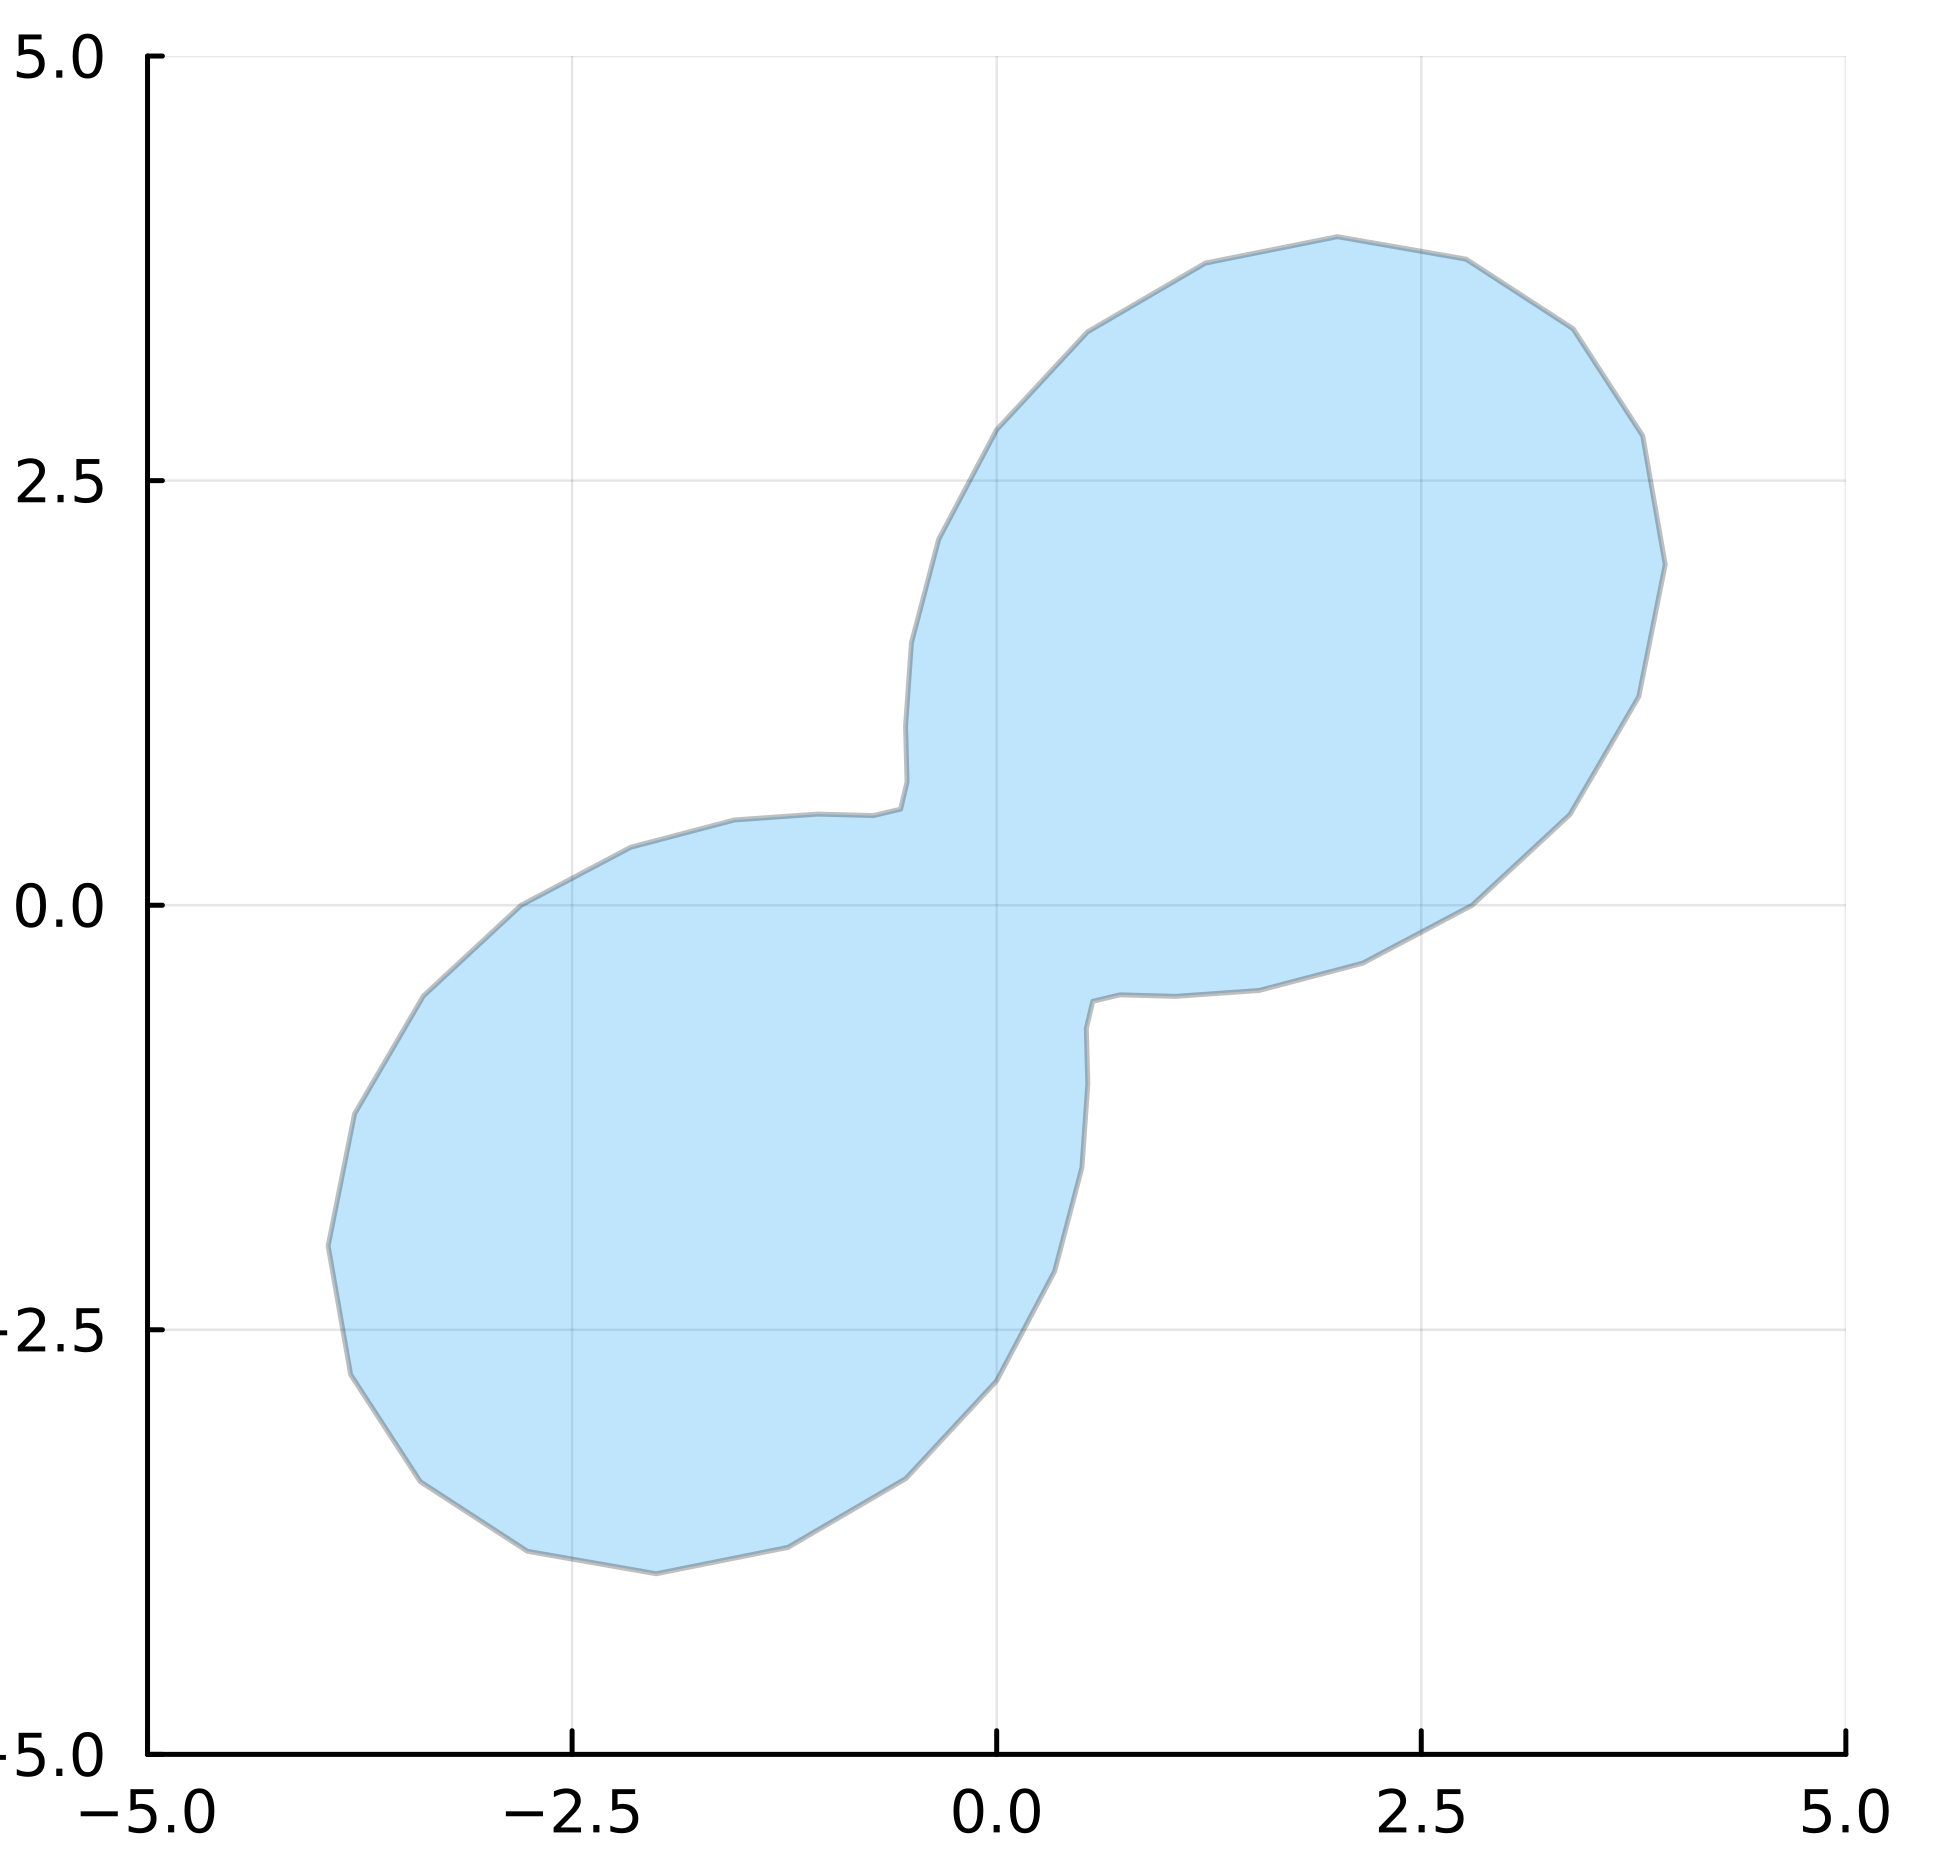
\includegraphics[width=\textwidth]{forces/shapes/desired.png}
	\end{subfigure}

	\caption{The left figure shows the initial state and the right figure shows the desired state for the ODE, which tests the three overlap, edge and interior angle forces for their ability to restore a cell shape. Both cells have an amount of 40 vertices.}
	\label{fig:shaperrrs}
\end{figure}

On the one hand, the cell is initially identical to the rectangle $[-3,3]\times[-1,1]$ with an area of 12. We have 11 vertices on each edge, which are evenly distributed in relation to the individual edges. The total amount of vertices is still 40, because each vertex at a rectangle corner is located on two different rectangle edges. This results in edge lengths of 0.6 on the horizontal cell edges and 0.2 on the vertical cell edges. 
Except for the corner points of the rectangle, where the interior angles are 90°, every other vertex has an interior angle of 180°. \\
On the other hand, we have got the desired shape that looks like a peanut. The  area is roughly 29.2. The edges near the centre point $(0,0)$, with a minimum length of ca. 0.16, are smaller  than the peripheral edges, with a maximal edge length of ca. 0.80. The two vertices closest to the centre have an interior angle of about 243°, while the other interior angles decrease rapidly toward the outer cell regions, reaching a minimum value of 156°. \\
So, almost all cell parameters are quite different between the two states. \\
The ODE, that we will now apply on the initial state's vertices, reads
\begin{model} \textbf{Discrete shape recovery model} \\
	The discrete shape recovery model is given by
	\begin{align}
		\dfrac{d \vec{x}_j}{d t} = F^{(A)}_j(C) + F^{(E_j)}_j(C) +F^{(I_j)}_j(C) \label{eq:shapeRecovery}. 
	\end{align}
	It uses the first three energies that operate on single cells. 
\end{model}

with the first three forces from the previous paragraphs. 
\begin{figure}[h!]
	\begin{center}
		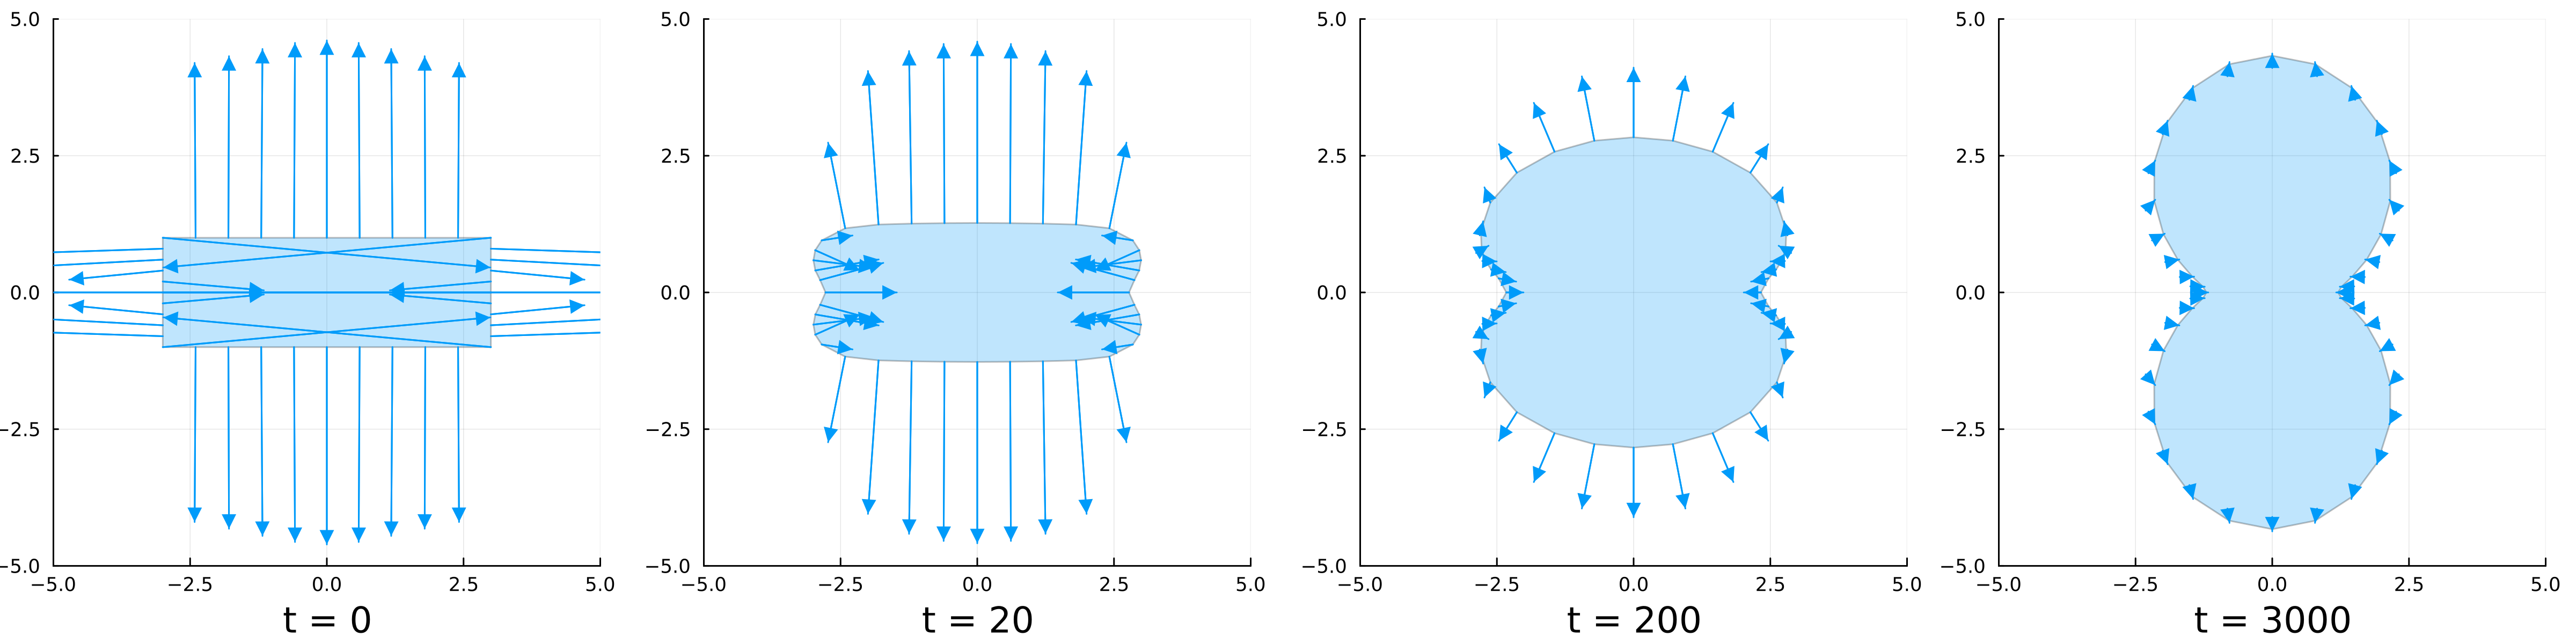
\includegraphics[width=15cm]{forces/shapes/shapes1.png}
		\caption{This series of plots shows the solution to the ODE just explained. For $t=0$, we can see the initial condition from Figure \ref{fig:shaperrrs} and the forces that initially act on the vertices. The following three diagrams show the solutions at the times $t \in \{20, 200, 3000\}$. They show a good transition from the starting shape into the desired state. }
		\label{fig:shapeShifteros}
	\end{center}
\end{figure}
The solution can be seen in Figure \ref{fig:shapeShifteros}. The result at $t=3000$ is congruent to the desired state, but it took a lot of time steps to get there. For $t>500$, the acting forces are really weak, although the desired state is not finally reached. The transformation is quite slow at the end. The reason therefor could be that the scaling factors in the area-, edge- and interior angle terms got smaller and smaller, because the shape got closer to the desired shape.\\
It is also noticeable that the final cell shape from the ODE solution is congruent, but rotated by 45°. The reason for this is, that no force has an impact on the cells rotation, but only on the characteristics area, edge lengths and interior angles. As long as these values are met as required, no further force is exerted. \\
All in all, it is a good result that the forces can manage the cell transformation into a specific shape, even though the initial situation is quite different. \\

\subsection{Interactive system}
Now, we can start the consideration of the interactive system with overlap energy. Therefor, we will now consider a system of $M=9$ DF cells with $N=20$ vertices each. Since the focus is now set on the overlap energy and not on the shape recovery, we set the desired cell shape equal to the initial shape. Thus, only cell deformations caused by the overlapping forces should be regenerated into the desired shape.\\
We choose the initial condition as shown in the first diagram of Figure \ref{fig:interactionSnippets}. All cells have the same shape and are concentrated on the bottom left corner of our domain $G$. The cells are initially arranged in such a way that there is a lot of overlap to show how the overlap energy affects the dynamics.\\
There are some terms that we must add to the ODE, in order to get a useful simulation. \\
First of all, we want every cell to move around. Thus, every cell should perform a random Brownian motion like in the papers from Bruna and Chapman in the introduction. This turns our previously deterministic ODE into a stochastic differential equation (SDE). In every time step, a normally distributed vector is generated for each cell, that gives it a random motion. Every vertex from the same cell gets the same Brownian motion applied such that the cell shape as a whole is not influenced, but only the cell position. We choose a diffusion constant of $D=2$. \\
On top, we will do a rescaling for our forces. Simulations without a rescaling do not show a big impact. But since we especially want our overlap force to have an impact as soon as two cells overlap, we multiply its force by a factor of ten. In summary, we obtain the SDE
\begin{model} \textbf{First interacting system} \label{model:interaction1}\\ 
	The sum of all derived forces yields the first interacting system
	\begin{align}
		d\vec{x}_{ij}(t) =  F^{(A_i)}_j(C_i) + F^{(E_{ij})}_j(C_i) +F^{(I_{ij})}_j(C_i) +10 F^{(O_i)}_j(C_i) + \sqrt{2D} dB_t^{(i)}, \label{eq:interaction1}
	\end{align}
	where $\vec{x}_{ij}$ again stands for the vertex $j$ of the $i$th cell, $(1\leq i \leq9, \; 1\leq j \leq 20)$. 
\end{model}
Except for the last addend, which makes up the stochastic part of the SDE, all other addends belong to the deterministic part.
Figure \ref{fig:interactionSnippets} shows snippets of the solution. 
\begin{figure}[h!]
	\begin{center}
		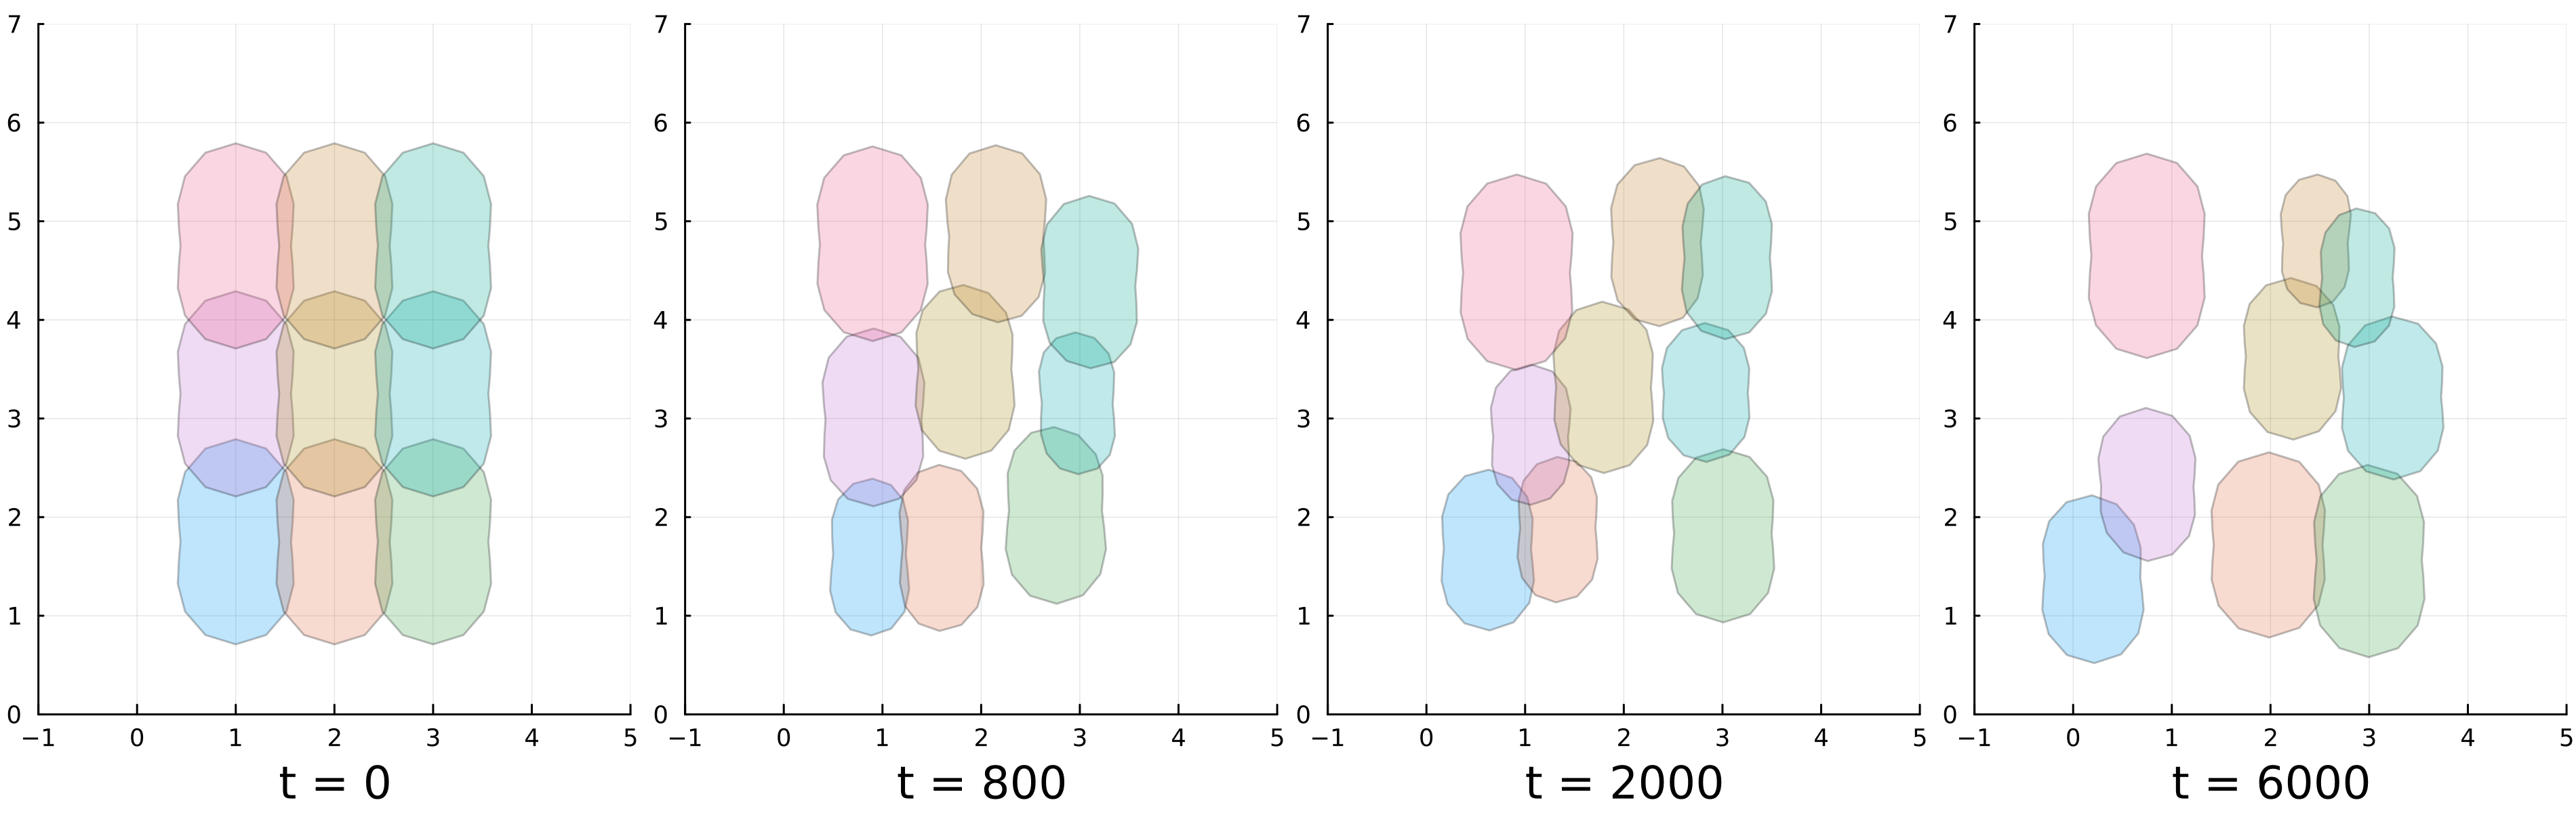
\includegraphics[width=15cm]{forces/interaction/overlapx10/overlapx10.png}
		\caption{Here, we can see a solution to the described SDE \eqref{eq:interaction1} with a rescaled overlap force by the factor of 10. The solution is shown at the times $t \in \{ 0, 800, 2000, 6000\}$.}
		\label{fig:interactionSnippets}
	\end{center}
\end{figure}
It is hard to show the important processes in this simulation with just a few frames, but this should give a good intuition. One can see that in situations where the Brownian motion causes heavy collisions between different cells, the overlap force starts acting and minimizes the overlapping area. Despite of this working well, we can see in this simulation, that the cells seem to be too static. It looks like, it is not just the area in the overlap, that gets minimized, but the cell as a whole. The reason therefor is probably that the interior angle force is too large, causing a lack of cell flexibility, because the shape cannot change, since the interior angles stay the same. We can also see that the influence of the area force is too small. \\
So let us take a look at another simulation with a different scaling for the force functions. We consider the SDE
\begin{model} \textbf{Rescaled interacting system} \label{model:interaction2}\\
	A rescaling of Model \ref{model:interaction1} yields the rescaled interacting system
	\begin{align}
		d\vec{x}_{ij}(t) =  50 F^{(A_i)}_j(C_i) + 1.5 F^{(E_{ij})}_j(C_i) + F^{(I_{ij})}_j(C_i) + 80 F^{(O_i)}_j(C_i) + \sqrt{2D} dB_t^{(i)}. \label{eq:interaction2}
	\end{align}
\end{model}


A solution to this SDE is illustrates in Figure \ref{fig:interaction_rescaled}. 
\begin{figure}[h!]
	\begin{center}
		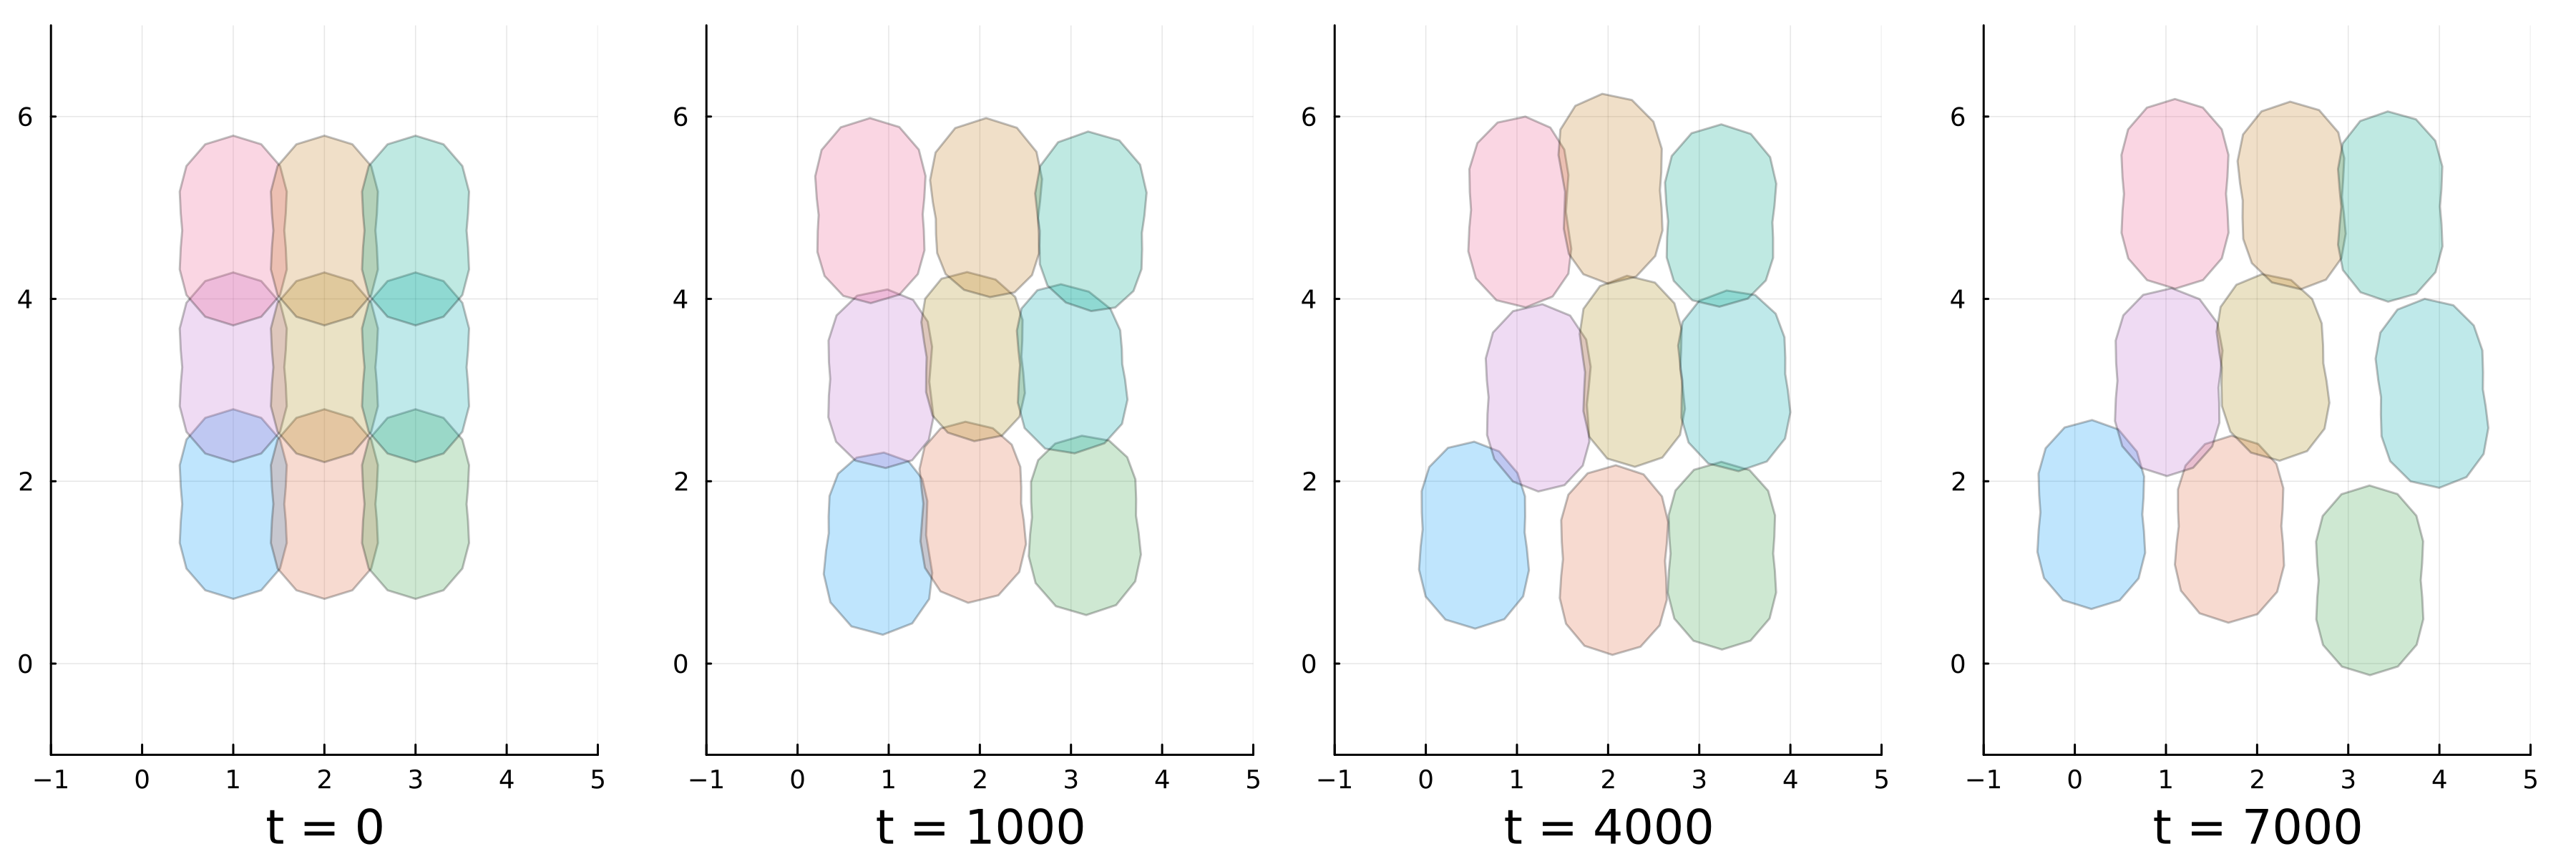
\includegraphics[width=15cm]{forces/interaction/interaction_rescaled/interaction_rescaled.png}
		\caption{This figure shows different plots of a solution to the explained SDE \eqref{eq:interaction2} with the rescaled force configuration. We can see the cells at the times $t \in \{ 0, 1000, 4000, 7000\}$. }
		\label{fig:interaction_rescaled}
	\end{center}
\end{figure}
In fact, we can see some differences to the first SDE and exactly the desired effect occurred. Each cell is more flexible and has a slightly different shape compared to the others. It is not just the general cell size that changes. The flexibility makes it possible to resolve the overlap more quickly, as the free spaces are better used by the cells to expand into. The interaction effect between the cells looks much smoother, because the different cell walls fit very tightly together. \\
We can conclude that a higher scaling factor for the edge and interior angle forces implies that the cells get more static and less adaptable to changes in the cell shape. \\
In summary of the interactive system, we can say that we have succeeded in creating a dynamic that is able to resolve overlaps while also maintaining a desired cell structure. In the absence of the overlap, the simulation from Subsection \ref{par:shapeRecovery} has shown that even strong shape changes can be regenerated back to the desired state by the cell-internal area, edge and interior angle forces.



\newpage
\section{Conclusion}
This bachelor thesis can be divided into two sections. The goal of the first part is to develop cell models that are able to represent complex shapes. \\
In Chapter \ref{sec:CellDef}, we derive the two cell forms that are the centre radius form (CRF) and the discrete form (DF). \\
The CRF is continuous in the sense that it contains the information for each point of the cell wall. Using the CRF one is able to represent every star shaped cell form. For the computation of the cell area, we introduced the smooth indicator function. It uses the data from a CRF and can determine if any point $\vec{x} \in \R^2$ is inside of the cell or not. It has similarities to the phase field model from \cite{Happel2023}. As the name suggests, the smooth indicator function of a cell can be used to calculate the cell area or the cell overlap of several cells via an integral using the product of their smooth indicator functions, just as it would be possible with the normal indicator function. \\
However, DF cells are a sequence of $N \in \N$ vertices that form a polygon when connecting adjacent vertices. As simple as the approach is, the possibilities for establishing cell dynamics are just as great. While calculating the area is easy using the shoelace formula, determining the overlap between 2 DF cells requires a complex algorithm. \\
After introducing the cell models and deriving area and overlap calculations, the foundation for the development of cell dynamics is laid, which leads us to the second main section of this work. \\
For the CRF model, we have found an ODE that can smoothly transform a cell from a certain initial state $C^{(0)}$ into a desired CRF $C^{(1)}$ in Section \ref{sec:ShapeRecoveryModel}. There are no further extensions developed for CRF dynamics. \\
Instead, the focus in the following is on the dynamics of the DF cells in Section \ref{sec:energyModels}. Here, we examine various energy functions that measure specific energy potentials within a cell or between different cells. With the usage of gradient flows, we could derive forces from the energy that got applied onto the cells vertices in order to reduce the energies. This procedure is similar to that from the paper \cite{Fletcher14}. After examining each force individually, we begin to combine the forces, resulting in a serviceable dynamic with interactions of an entire cellular system. \\
Of course there are some meaningful extensions for my thesis. \\
In order to compute solutions to the energy dynamics, I have just used an explicit Euler method for the deterministic differential equations and Euler Maruyama schemes for the stochastic differential equations with a fixed time step size of $\Delta t = 2^{-8}$. Other methods, e.g. methods with adaptive time stepping, are suited better for computing more accurate solutions at times when rapid changes to the solution occur. \\
If needed, it is also possible to introduce new energies and forces into the energy based system. For example, if the cell's rotation plays an important role, one could implement a force, that makes the cell rotate into a certain position. \\
The rescalings, showed at the end of Chapter \ref{sec:energyModels}, are just possible examples of scalings. Depending on the desired cell properties, like for example deformability, other scalings may be preferred. \\
Another possible use case could be to define a domain $\Omega$ such that cells are not allowed to leave it. This could be implemented with a further force function $F^{(B)}$ `boundary push' that pushes the whole cell back into the domain, if it touches the boundary $\partial \Omega$. \\
In \cite{Bruna2023} Bruna, Chapman and Schmidtchen studied a macroscopic model for Brownian hard needles. Similar to the hard sphere model in the paper \cite{Bruna2012} from the introduction, there are exclusion effects for the different needle particles. The authors managed to derive an effective PDE that describes the probability density $\rho(t,\vec{x}, \theta)$ of finding a needle with rotation $\theta$ at position $\vec{x}$ and time $t$. An interesting next step for the development of the theory in this thesis would be to derive an effective PDE for our energy dynamic model of the DF cells. \\
Another problem could be the elaborate computation of the discrete cell overlap. Here, one could try to find faster algorithms to solve this. If the setup allows it, assuming convex polygons could simplify some calculations. An approach, that I tried to implement, does not determine every edge of the cell, but only those at critical areas. It is explained in the appendix \ref{sec:appendix}. The approach worked in most cases, but unfortunately there are also configurations where the algorithm failed if one does not take further assumptions. Since these situation are mostly made up, it could be possible to deploy this ansatz. 

\newpage
\section*{Appendix} \label{sec:appendix}
\subsection*{An attempt to simplify the discrete overlap computation}
\begin{figure}[b!]
	
	\centering
	\begin{subfigure}{0.4\textwidth}
		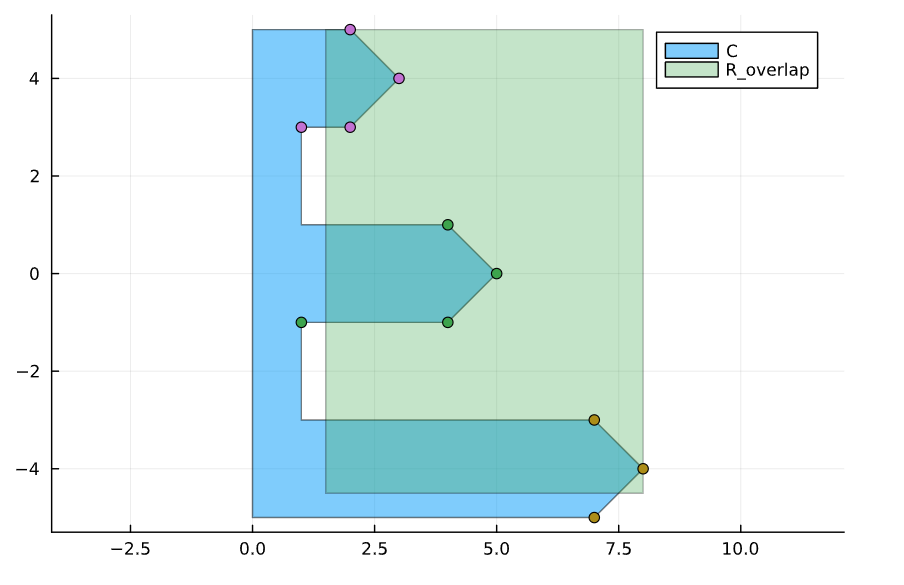
\includegraphics[width=\textwidth]{discreteOverlap/finding_lists_in_rectangle.png}
		\caption{Here, we only concentrate on the cell $C$ and $R_{overlap}$. Every vertex is associated with the counterclockwise next edge. The cell intersects the rectangle multiple times, causing several critical lists. Each of the three list is marked with its own colour. Only critical edges are marked with a dot. }
		\label{fig:criticalLists1}
	\end{subfigure}
	\hfill
	\begin{subfigure}{0.4\textwidth}
		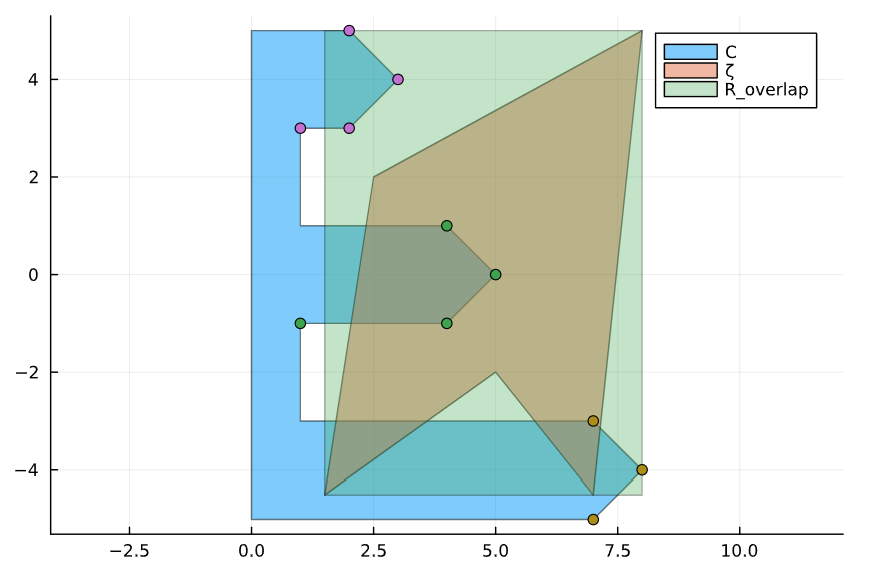
\includegraphics[width=\textwidth]{discreteOverlap/finding_lists_in_rectangle2.png}
		\caption{Now, we can also see the second discrete cell $\zeta$. There are three areas where both cells overlap. Note that although the orange critical list takes part in two overlaps, it is does not happen that two different critical lists of the same cell involve in the same overlap.}
		\label{fig:fig:criticalLists2}
	\end{subfigure}
	
	
	\caption{Here, we can see a pattern of two cells $C$ and $\zeta$ and the domain $R_{overlap}$. This figure gives a perception of critical lists and what they are used for. }
	\label{fig:criticalLists}
	
\end{figure}
While researching the implementation of calculating the overlap of two DF cells in the Chapter \ref{sec:ImplementationDiscreteOverlap}, I also focused on an idea to simplify the Problem \ref{problem:overlap} and reduce the computational effort. \\
Unfortunately, I discovered counterexamples that contradicted my idea. However, since these counterexamples are rather artificial, this method may still have a right to exist. Perhaps, one can figure out how to circumvent the problem of the counterexample. One could also add constraints to the model, e.g. that only convex cells are regarded or that all occurring overlaps are convex. \\
In difference to the showed algorithm in the Chapter \ref{sec:ImplementationDiscreteOverlap}, not every cell edge is critical. We choose the following definition. 
\text{} \\  
\textbf{Definition. Critical edge} \\
Let $C$ and $\zeta$ be two overlapping DF cells and $R_{overlap}$ the smallest rectangle that covers all overlap areas. Than any edge is considered to be critical if it intersects with $R_{overlap}$. 
\text{} \\  
The concept is only to consider lists of consecutive edges that are located in the critical area $R_{overlap}$. \\
\text{} \\  
\textbf{Definition. Critical list} \\
A critical list is an ordered, maximal list $L = (l_1, \ldots, l_L) = (e_i, e_{i+1}, \ldots, e_M)$ of critical edges such that all edges in the list are consecutive. Maximal means one cannot add another consecutive critical edge before or at the end of $L$. \\
\text{} \\  
I was hoping that each intersection of the two cells is always build with edges of just one critical list per cell.
Then, the original Problem \ref{problem:overlap} could have been simplified to the following problem.\\
\text{} \\  
\textbf{Problem.} \\
For given critical lists $L$ from $C$ and $\lambda$ from $\zeta$, determine all discrete cells $O_1, \ldots, O_K$ such that any overlap that uses edges of $L$ and $\lambda$ is represented by exactly one $O_k$ $(k \in 1, \ldots, K)$. 
\text{} \\  
Figure \ref{fig:failedLists} shows an example of two DF cells that have an overlap which uses edges of two different critical lists of the same cell. After finding that out, I decided to consider every edge to be critical and developed the procedure that is found in Chapter \ref{sec:ImplementationDiscreteOverlap}. 
\begin{figure}[h!]
	\centering
	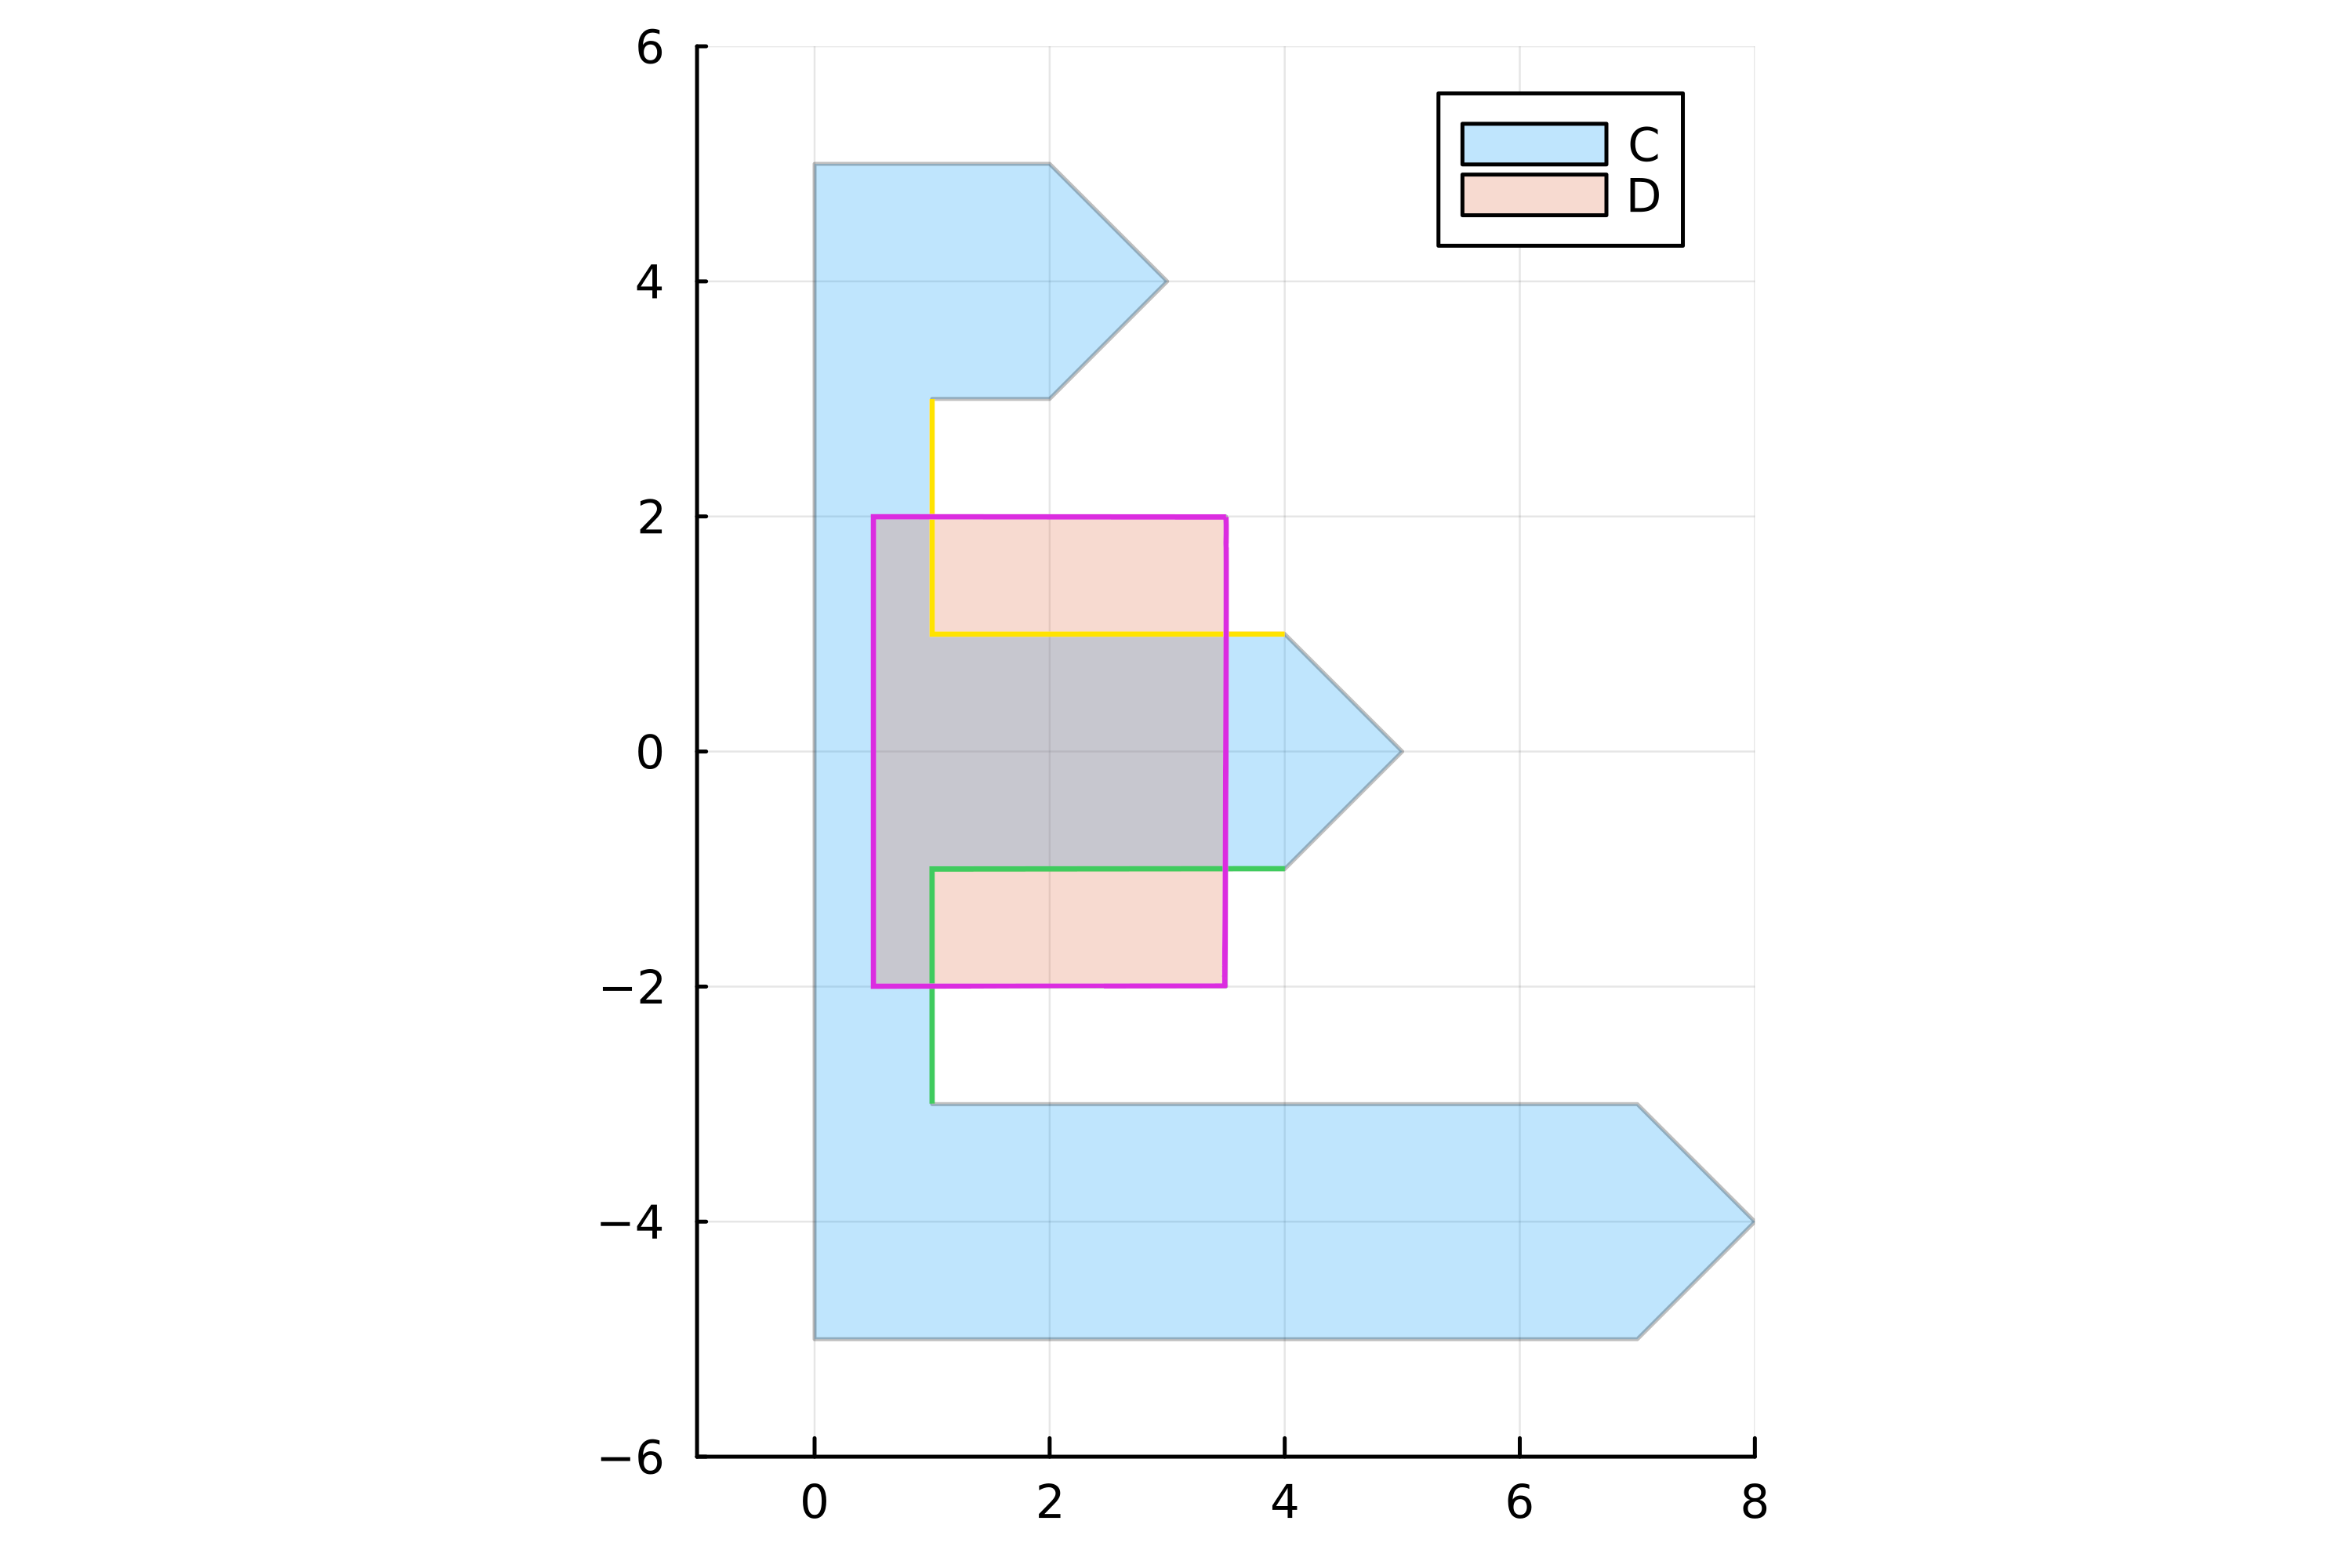
\includegraphics[width=8cm]{ApproachFailure.png}{}
	\caption{This plot shows a configuration of two DF cells $C$ and $D$. The rectangle $R_{overlap}$ is identical to $D$ in this case. Thus, each edge of $D$ is critical and we obtained one critical list for $D$ that is shown in pink. For $C$ we get two critical lists that are shown in yellow and green. We have got one overlap between $C$ and $D$ and it uses edges from each the green and the yellow critical list of $C$.}
	\label{fig:failedLists}
\end{figure}


\newpage
\bibliography{quellen}


\newpage
%%
%% Erscheint auf letzter Seite
%%
\section*{Statement of authorship}
\thispagestyle{empty}

I hereby declare that I have written this thesis (\emph{\thema}) under the supervision of Jun.-Prof. Dr. Markus Schmidtchen independently  and have listed all used sources and aids. I am submitting this thesis for the first time as part of an examination. I understand that attempted deceit will result in the failing grade „not sufficient“ (5.0). \\
\bigskip


\bigskip \bigskip  

\vspace{10mm}
\begin{tabular}{@{}p{2.5in}@{}}
	\hrulefill \\
	Tim Vogel\\
	Dresden, \datum\  \\
	Technische Universität Dresden \\
	Matriculation Number: 4930487 \\
\end{tabular}


\normalsize
\end{document}







\paragraph{Case distinction for critical edges}
With these preparations, we are now ready to determine whether an edge is critical or not for $R_{overlap}$. We will call the boundary coordinates of $R_{overlap}$ $r_x^{min}$, $r_x^{max}$, $r_y^{min}$ and $r_y^{max}$. 
If the starting or ending vertex ($x_i$ or $x_{i+1}$) of $e_i$ lays in the rectangle, it follows directly from the definition that $e_i$ is \textbf{critical}. \\
If the edge is not located near the rectangle, i.e. if at least one the following cases is true,
\begin{center}
	$x_i^{min} > r_x^{max}$, \\
	$x_i^{max} < r_x^{min}$, \\
	$y_i^{min} > r_y^{max}$, \\
	$y_i^{max} < r_y^{min}$,
\end{center}
we know that the edge is \textbf{not critical}. \\
Having checked these states first, we now assume that the four cases mentioned right above are all false. 
Then, we can directly conclude that edges which run completely horizontally ($m_i = 0$) or vertically (a not parameterisable edge) will always cut $R_{overlap}$ and be \textbf{critical}. Otherwise, one of the four conditions would have to be true. \\
In all remaining instances, the edge is parameterisable and the path is not a constant function. Thus, $m_i$ and $a_i$ exist and $m_i \neq 0$. Next, we check whether it cuts the rectangle at the vertical sides. 
\begin{center}
	$e_i$ intersects $R_{overlap}$ on the left vertical side \\
	$\iff  r_x^{min} \in [x_i^{min}, x_i^{max}] \: \land \: m_i r_x^{min} + a_i \in [r_y^{min}, r_y^{max}]$,\\
	\bigskip
	$e_i$ intersects $R_{overlap}$ on the right vertical side \\
	$\iff  r_x^{max} \in [x_i^{min}, x_i^{max}] \: \land \: m_i r_x^{max} + a_i \in [r_y^{min}, r_y^{max}]$.
	
\end{center}
The edge $e_i$ is \textbf{critical} if one of these statements is true.\\
Whenever this is not the case, $e_i$ can only be \textbf{critical} if and only if it cuts one of the horizontal rectangle sides. Therefor, we first determine the $x$ coordinate $t$ where the edge reaches the height of the top or bottom rectangle side. Then, we check if this $t$ is in the right area. Insert $r_y^{min}$ or respectively $r_y^{max}$ for $r_y$. 
\begin{center}
	
	$m_i t + a_i = r_y \iff  t = \dfrac{r_y - a_i}{m_i}$  \\
	\bigskip
	$e_i$ intersects $R_{overlap}$ on the considered horizontal side \\
	$\iff t \in  [x_i^{min}, x_i^{max}]$.\\
	
\end{center}
If this is still not the case, the edge must be \textbf{not critical}. \\
$\smallskip$\\
So, we can now decide for any given edge and rectangle if the edge is critical or not. This is one important point for the calculation of the overlapping cells. The next step is to find all lists of consecutive critical edges. \\


As we will see from now on, critical lists are another stage for the solution of Problem \ref{problem:overlap}. We must get from two bigger discrete cells to possibly multiple smaller overlap cells and discrete lists are some kind of a first break down of the bigger origin cells. \\


\paragraph{Algorithm for the computation of the overlap}
\begin{algorithm} \textbf{Compution of Overlaps of Critical Lists} 
	
	\begin{itemize} 
		\itemsep0em 
		\item[] \text{INPUT:}
		\item Critical list $L$ of $C$
		\item Critical list $\lambda$ of $\zeta$ 
		\item List $I$ of all intersections in $L$ and $\lambda$ 
	\end{itemize}
	
	\begin{algorithmic}
		
		\Function{collectOverlaps}{L, $\lambda$, I}
		
		\State O = empty Set 
		\While{I is not empty}
		
		\State newO, usedI = constructOverlap($L$, $\lambda$, $I$)
		\State O = O $\cup$ {newO}
		\State I = I $\setminus$ usedI 
		
		\EndWhile
		
		\Return O
		
		\EndFunction
		\\
		\Function{constructOverlap}{$L$, $\lambda$, $I$}
		\\
		\Comment{Always uses the first element I[1] as starting intersection}
		
		\State usedI = List{Points}(I[1]) 
		\State newO = DiscreteCell(i1) 
		\State currentI = I[1]
		\For{counter = 1 : length(I)} 
		
		\If{counter is even}
		
		\State pathC, newI = findPath(currentI, L) 
		
		\Else 
		
		\State pathC, newI = findPath(currentI, $\lambda$) 
		
		\EndIf
		
		\State append!(newO, pathC)
		\If{newI == I[1]} 
		\State \Return newO, usedI
		\Else 
		\State append!(newO, newI)
		\State append!(usedI, newI) 
		\EndIf
		
		\EndFor
		\EndFunction
		\\
		\Function{findPath}{currentI, L} 
		
		\State Goes in the right list direction until it finds the next 
		\State intersection which will be newI. Until then all cell wall 
		\State will be saved in path
		
		
		\Return path, newI
		\EndFunction 
		
	\end{algorithmic}
	
	\begin{itemize} 
		\itemsep0em 
		\item[] \text{OUTPUT:}
		\item Set $O = (O_1, \ldots, O_K)$ like in Problem \ref{problem:list} 
	\end{itemize}
	
	
	
	
\end{algorithm}
